%----------------------------------------------------------------------------------------
%    PACKAGES AND OTHER DOCUMENT CONFIGURATIONS
%----------------------------------------------------------------------------------------

% Choose the language
\ifxetexorluatex
    \usepackage{polyglossia}
    \setmainlanguage[variant=american]{english}
\else
    \usepackage[english]{babel} % Load characters and hyphenation
\fi
\usepackage[english=american]{csquotes}    % English quotes

% Load the bibliography package
\PassOptionsToPackage{
    natbib=true,
    datamodel=software,
}{biblatex}
\usepackage[addspace=false]{kaobiblio}

\usepackage{software-biblatex}
\ExecuteBibliographyOptions{
    halid=false,
    swhid=false,
    swlabels=false,
    vcs=true,
    license=true
}

\addbibresource[label=ownpubs]{bib/00_own_publications.bib}
\addbibresource[label=ownsoft]{bib/01_own_software.bib}
\addbibresource[label=main]{bib/02_phd_thesis.bib}
%\addbibresource[label=ownpubs,location=remote]{http://127.0.0.1:23119/better-bibtex/export?/library;name:My%20Library/collection/00_own_publications.biblatex.biblatex&useJournalAbbreviation=true}
%\addbibresource[label=ownsoft,location=remote]{http://127.0.0.1:23119/better-bibtex/export/collection?/1/01_own_software.biblatex&useJournalAbbreviation=true}
%\addbibresource[label=main,location=remote]{http://127.0.0.1:23119/better-bibtex/export/collection?/1/02_phd_thesis.biblatex&useJournalAbbreviation=true}
%\addbibresource[label=filter_function_paper,location=remote]{http://127.0.0.1:23119/better-bibtex/export/collection?/1/03_filter_function_paper.biblatex&useJournalAbbreviation=true}

%----------------------------------------------------------------------------------------
% Custom packages
%----------------------------------------------------------------------------------------
%\usepackage{pdfpages}
\PassOptionsToPackage{
    chapter,%
    cache=true,%
}{minted}
    \usepackage{minted}

\setminted[python]{
    fontfamily=tt,% tt,courier,helvetica
    style=gruvbox-light,%gruvbox-light,github-light,default
}

\newminted[py]{python}{
    autogobble=true,%
    frame=leftline,% none | leftline | topline | bottomline | lines | single
    fontsize=\small,% normalsize, small, footnotesize
    linenos=false,
    firstnumber=last,% line number counts incrementally
}
\newmintinline[pyinline]{python}{
    breaklines,%
    breakafter=._,%
}

\usepackage{lettrine}
%\usepackage{Zallman}
%\usepackage{Starburst}
%\usepackage{Rothdn}
% Use these like so:
% \Zallmanfamily
\renewcommand{\LettrineFontHook}{\fontspec{Libertinus Serif Initials}\color{RWTHblue100}}

\usepackage{tabularx} % better tables with given width
\usepackage{threeparttable} % tablenotes env
%\setlength{\extrarowheight}{3pt} % increase table row height
\usepackage{collcell} % for verb columns

\usepackage{fontawesome5} % fancy icons

%! begin preamble = tikz
% graphs
\usetikzlibrary{
    arrows,
    positioning,
    calc,
    angles,
    quotes,
    shadows,
    decorations.markings
}
% tree structures
\usepackage[edges]{forest}
% electric circuits
\usepackage{circuitikz}

%\usepackage{pgfplots}
%\pgfplotsset{compat=1.18}

% Fix for matplotlib's PGF backend
% https://github.com/matplotlib/matplotlib/issues/27907
\newcommand{\mathdefault}[1]{\displaystyle #1}

%\usetikzlibrary{math}
% quantum circuits
\usetikzlibrary{quantikz2}

% cache pdfs, needs shell-escape. does not work on linux 18/04
%\usetikzlibrary{external}
%\tikzexternalize[prefix=img/pdf/]
%! end preamble = tikz

%! begin preamble = math
\usepackage{dsfont}
\RequirePackage{mathtools}
%\usepackage{mathrsfs}
\usepackage{chemformula}
\usepackage{physics}
\usepackage{siunitx}
\sisetup{per-mode = single-symbol}
\AtBeginDocument{\RenewCommandCopy\qty\SI}
%! end preamble = math
%----------------------------------------------------------------------------------------
% Config
%----------------------------------------------------------------------------------------
% Margin TOC
%\setcounter{margintocdepth}{\sectiontocdepth}
% Use like so:
% \setchapterpreamble[u]{\margintoc}
% \chapter{foo}
% This would be nice to have for parts, but those don't have margins atm.
%\counterwithin*{chapter}{part}

% Make cleveref use "Appendix" instead of "Chapter" after \appendix
% https://github.com/latex3/hyperref/issues/362
\AddToHook{cmd/appendix/before}{\crefalias{chapter}{appendix}}

%----------------------------------------------------------------------------------------
% Load mathematical packages for theorems and related environments
\usepackage[framed=true]{kaotheorems}

% Load the package for hyperreferences
\usepackage{kaorefs}

\graphicspath{ {./img/}{./} } % Paths in which to look for images

% \makeindex[columns=3, title=Alphabetical Index, intoc] % Make LaTeX produce the files required to compile the index

\makeglossaries % Make LaTeX produce the files required to compile the glossary
\usepackage{glossaries}\newglossaryentry{computer}{
	name=computer,
	description={is a programmable machine that receives input, stores and manipulates data, and provides output in a useful format}
}

% Glossary entries (used in text with e.g. \acrfull{fpsLabel} or \acrshort{fpsLabel})
\newacronym[longplural={Frames per Second}]{fpsLabel}{FPS}{Frame per Second}
\newacronym[longplural={Tables of Contents}]{tocLabel}{TOC}{Table of Contents}

\newacronym{rb}{RB}{randomized benchmarking}
\newacronym{srb}{SRB}{standard randomized benchmarking}
\newacronym{irb}{IRB}{interleaved randomized benchmarking}
\newacronym{gst}{GST}{gate set tomography}
\newacronym{qpt}{QPT}{quantum process tomography}
\newacronym{qec}{QEC}{quantum error correction}
\newacronym{se}{SE}{spin echo}
\newacronym{ptm}{PTM}{Pauli transfer matrix}
\newacronym{me}{ME}{Magnus expansion}
\newacronym{dd}{DD}{dynamical decoupling}
\newacronym{dcg}{DCG}{dynamically corrected gate}
\newacronym{ff}{FF}{filter function}
\newacronym{mc}{MC}{Monte Carlo}
\newacronym{cff}{CFF}{correlation filter function}
\newacronym{qft}{QFT}{quantum Fourier transform}
\newacronym{cp}{CP}{completely positive}
\newacronym{povm}{POVM}{positive operator-valued measure}
\newacronym{iid}{i.i.d.}{independent and identically distributed}
\newacronym[longplural={power spectral densities}]{psd}{PSD}{power spectral density}
\newacronym[longplural={cross power spectral densities}]{csd}{CSD}{cross power spectral density}
\newacronym[longplural={amplitude spectral densities}]{asd}{ASD}{amplitude spectral density}
\newacronym{enbw}{ENBW}{equivalent noise bandwidth}
\newacronym{tlf}{TLF}{two-level fluctuator}
\newacronym{rms}{RMS}{root mean square}
\newacronym{daq}{DAQ}{data acquisition}
\newacronym{dac}{DAC}{digital-to-analog converter}
\newacronym{adc}{ADC}{analog-to-digital converter}
\newacronym{tia}{TIA}{transimpedance amplifier}
\newacronym{lia}{LIA}{lock-in amplifier}
\newacronym{fft}{FFT}{fast Fourier transform}
\newacronym{dut}{DUT}{device under test}
\newacronym{api}{API}{Application Programming Interface}
\newacronym{gui}{GUI}{graphical user interface}
\newacronym{dr}{DR}{dilution refrigerator}
\newacronym{ptr}{PTR}{pulse tube refrigerator}
\newacronym{sem}{SEM}{Scanning electron microscope}
\newacronym{pt1}{PT1}{first pulse tube stage}
\newacronym{pt2}{PT2}{second pulse tube stage}
\newacronym{mxc}{MXC}{mixing chamber}
\newacronym{sma}{SMA}{SubMiniature version A}
\newacronym{bnc}{BNC}{Bayonet Neill–Concelman}
\newacronym{dmm}{DMM}{digital multimeter}
\newacronym{smf}{SMF}{single-mode fiber}
\newacronym{mmf}{MMF}{multi-mode fiber}
\newacronym{ebl}{EBL}{electron-beam lithography}
\newacronym{tem}{TEM}{transverse electromagnetic}
\newacronym{te}{TE}{transverse electric}
\newacronym{qw}{QW}{quantum well}
\newacronym{apd}{APD}{avalanche photodiode}
\newacronym{spcm}{SPCM}{single-photon counting module}
\newacronym{pde}{PDE}{photon detection efficiency}
\newacronym{hbt}{HBT}{Hanbury Brown-Twiss}
\newacronym{cmos}{CMOS}{complementary metal-oxide-semiconductor}
\newacronym[longplural={vibration criteria}]{vc}{VC}{vibration criterion}
\newacronym{iso}{ISO}{International Organization for Standardization}
\newacronym{snr}{SNR}{signal-to-noise ratio}
\newacronym{ar}{AR}{anti-reflection}
\newacronym{bbar}{BBAR}{broadband anti-reflection}
\newacronym{nir}{NIR}{near-infrared}
\newacronym{na}{NA}{numerical aperture}
\newacronym{ca}{CA}{clear aperture}
\newacronym{wd}{WD}{working distance}
\newacronym{mfd}{MFD}{mode field diameter}
\newacronym{bs}{BS}{beam splitter}
\newacronym{ccd}{CCD}{charge-coupled device}
\newacronym{pcc}{PCC}{photonic crystal cavity}
\newacronym{los}{LOS}{line-of-sight}
\newacronym{qd}{QD}{quantum dot}
\newacronym{gdqd}{GDQD}{gate-defined quantum dot}
\newacronym{oaqd}{OAQD}{optically active quantum dot}
\newacronym{saqd}{SAQD}{self-assembled quantum dot}
\newacronym[longplural={two-dimensional electron gases}]{2deg}{2DEG}{two-dimensional electron gas}
\newacronym[longplural={two-dimensional hole gases}]{2dhg}{2DHG}{two-dimensional hole gas}
\newacronym{bob}{BOB}{break-out box}
\newacronym{pl}{PL}{photoluminescence}
\newacronym{ple}{PLE}{photoluminescence excitation}
\newacronym{cw}{cw}{continuous-wave}
\newacronym{tmm}{TMM}{transfer-matrix method}
\newacronym{blg}{BLG}{bilayer graphene}
\newacronym{tmd}{TMD}{transition-metal dichalcogenide}
\newacronym{od}{OD}{optical density}
\newacronym{qe}{QE}{quantum efficiency}
\newacronym{nd}{ND}{neutral-density}
\newacronym{pcb}{PCB}{printed circuit board}
\newacronym{soi}{SOI}{spin-orbit interaction}
\newacronym{bec}{BEC}{Bose-Einstein condensate}
\newacronym{qcse}{QCSE}{quantum-confined Stark effect}
\newacronym{fes}{FES}{Fermi-edge singularity}
 % Include the glossary definitions

% \makenomenclature % Make LaTeX produce the files required to compile the nomenclature
%----------------------------------------------------------------------------------------
% DEBUG
%----------------------------------------------------------------------------------------
%\usepackage{blindtext} % Print text without any meaning for testing purposes
%\usepackage{showframe} % Uncomment to show boxes around the text area, margin, header and footer
%\usepackage{showlabels} % Uncomment to output the content of \label commands to the document where they are used
%\usepackage{lipsum}

%\usepackage{printlen}
%\uselengthunit{in}
% Use:
% \printlength{\marginparsep}

%\ExplSyntaxOn
%\NewDocumentCommand{\thefontsize}{O{}}{#1 The current font size is:  \f@size \pt\par}
%\ExplSyntaxOff
% Use:
% \thefontsize\footnotesize
%----------------------------------------------------------------------------------------
\includeonly{
    tex/publications,
    tex/software,
%    chs/spectrometer/introduction,
%    chs/spectrometer/theory,
%    chs/spectrometer/software,
%    chs/spectrometer/conclusion,
%    chs/setup/introduction,
%    chs/setup/cooling.tex,
%    chs/setup/optics.tex,
%    chs/setup/vibrations,
%    chs/setup/conclusion,
    chs/experiment/introduction,
    chs/experiment/observations,
    chs/experiment/conclusion,
%    chs/filter_functions/introduction,
%    chs/filter_functions/prr,
%    chs/filter_functions/time_domain_methods,
%    chs/filter_functions/validation,
%    chs/appendices/setup/optics,
%    chs/appendices/setup/vibrations,
    chs/appendices/experiment/tmm,
%    chs/appendices/filter_functions,
}
% Language macros
\newcommand{\Ie}{\emph{I.\nobreak\hairsp{}e.\@}\xspace}
\newcommand{\Eg}{\emph{E.\nobreak\hairsp{}g.\@}\xspace}
\newcommand{\cf}{\emph{cf.\@}\xspace}
\newcommand{\Cf}{\emph{Cf.\@}\xspace}
\newcommand{\viz}{\emph{viz.\@}\xspace}
\newcommand{\wrt}{w.\nobreak\hairsp{}r.\nobreak\hairsp{}t.\@\xspace}
\newcommand{\ibid}{\emph{ibid.\@}\xspace}

% Text macros
\newcommand{\code}[1]{\pyinline{#1}}
\newcommand{\codev}[1]{\texttt{#1}}
\newcommand{\thepower}[2]{\ensuremath{P = \qty{#1}{#2\watt}}.\xspace}
\newcommand{\thevoltage}[2]{\ensuremath{V_{\mr{#2}} = \qty{#1}{\volt}}.\xspace}
\newcommand{\thewavelength}[1]{\ensuremath{\lambda_{\mr{exc}} = \qty{#1}{\nano m}}.\xspace} % XXX: \meter somehow causes an error

\newcommand{\thethesis}{the present thesis\xspace}
\newcommand{\thispart}{this part of \thethesis}
\newcommand{\Thispart}{This part of \thethesis}
% Instruments
\newcommand{\oxinst}{Oxford Instruments\xspace}
\newcommand{\odin}{\oxinst Triton 450\xspace}
\newcommand{\thedmm}{Keysight 34465A\xspace}
\newcommand{\swinst}{Swabian Instruments\xspace}
\newcommand{\taggershort}{Time Tagger\xspace}
\newcommand{\tagger}{\swinst \taggershort 20\xspace}
\newcommand{\thespcm}{Excelitas SPCM-850-14-FC\xspace}
\newcommand{\theccd}{Andor iDus 416\xspace}
\newcommand{\thespectrometer}{Horiba FHR1000\xspace}
\newcommand{\cmoscam}{Thorlabs DCC1545M \gls{cmos} camera\xspace}
\newcommand{\pumplaser}{Lighthouse Photonics Sprout-G\xspace}
\newcommand{\tisalaser}{M Squared Solstis\xspace}
\newcommand{\pulsedlaser}{Coherent Mira 900-F\xspace}
\newcommand{\accelerometer}{Wilcoxon 731--207\xspace}
\newcommand{\objectivelens}{Thorlabs 354330-B\xspace}
\newcommand{\ocularlens}{Thorlabs A280TM-B\xspace}
\newcommand{\thewindow}{Thorlabs WW41050-B\xspace}
\newcommand{\thorlabsrotator}{Thorlabs K10CR1/M\xspace}
\newcommand{\thorlabsflipper}{Thorlabs MFF101/M\xspace}
\newcommand{\thorlabspowermeter}{Thorlabs PM100D\xspace}
\newcommand{\thefiber}{Thorlabs 780HP\xspace}
\newcommand{\positioner}{Attocube ANPx311\xspace}
\newcommand{\rotator}{Attocube ECR4040\xspace}
\newcommand{\polarizer}{Thorlabs LPVIS050-MP2\xspace}
\newcommand{\polarizerunmounted}{Thorlabs LPVIS050\xspace}
\newcommand{\positionercontroller}{Attocube ANC350\xspace}
\newcommand{\rotatorcontroller}{Attocube AMC100\xspace}
\newcommand{\decadac}{DecaDAC\xspace}
\newcommand{\qdac}{QDevil QDAC-II\xspace}
\newcommand{\baselinst}{Basel Precision Instruments\xspace}
\newcommand{\baseltia}{\baselinst SP 983c\xspace}
\newcommand{\zhinst}{Zurich Instruments\xspace}
\newcommand{\hdawg}{\zhinst HDAWG\xspace}

% Software
\newcommand{\python}{Python\xspace}
\newcommand{\package}[1]{\nohyphens{\code{#1}}\xspace}
\newcommand{\pyspeck}{\package{python_spectrometer}}
\newcommand{\mjolnir}{\package{mjolnir}}
\newcommand{\qutil}{\package{qutil}}
\newcommand{\xarray}{\package{xarray}}
\newcommand{\filterfunctions}{\package{filter_functions}}
\newcommand{\qupulse}{\package{qupulse}}
\newcommand{\qopt}{\package{qopt}}
\newcommand{\qumada}{\package{QuMADA}}
\newcommand{\numpy}{\package{NumPy}}
\newcommand{\scipy}{\package{SciPy}}
\newcommand{\matplotlib}{\package{matplotlib}}
\newcommand{\qutip}{\package{QuTiP}}
\newcommand{\sparse}{\package{sparse}}
\newcommand{\opteinsum}{\package{opt_einsum}}
\newcommand{\jupyter}{\package{Jupyter}}
\newcommand{\qcodes}{\package{QCoDeS}}
\newcommand{\pymoosh}{\package{PyMoosh}}
\newcommand{\pulsesequence}{\code{PulseSequence}\xspace}
\newcommand{\pulsesequences}{\code{PulseSequence}s\xspace}
\newcommand{\qobj}{\code{Qobj}\xspace}
\newcommand{\slowprocessor}{AMD FX\texttrademark-6300 processor with six logical cores\xspace}
\newcommand{\fastprocessor}{Intel\textsuperscript{\textregistered}\ Core\texttrademark\ i9-9900K eight-core processor\xspace}

% Units
\DeclareSIUnit{\gaccel}{\mathit{g}}
\DeclareSIUnit{\cts}{cts}
\DeclareSIUnit{\cps}{cps}
\DeclareSIUnit{\sample}{S}
\DeclareSIUnit{\pixel}{px}
\DeclareSIUnit{\bar}{bar}
\DeclareSIUnit{\txtdegree}{deg}
\DeclareSIUnit{\permill}{\textperthousand}
\DeclareSIUnit{\electron}{\ensuremath{e}}

% Table macros
\newcolumntype{C}{>{\collectcell\code}c<{\endcollectcell}} % makes the whole column texttt style
\newcommand{\tableheadline}[1]{\multicolumn{1}{l}{\spacedlowsmallcaps{#1}}} % uses spacedlowsmallcaps borrowed from classicthesis

% Maths
\newcommand{\mc}[1]{\ensuremath{\mathcal{#1}}}
\newcommand{\mr}[1]{\ensuremath{\mathrm{#1}}}
\newcommand{\e}[0]{\ensuremath{e\xspace}}
\renewcommand{\i}[0]{\ensuremath{i\xspace}}
\newcommand{\eps}[0]{\ensuremath{\epsilon}\xspace}
\newcommand{\del}[0]{\ensuremath{\partial}}
\newcommand{\placeholder}[0]{\:\bullet\:}
\newcommand{\st}[0]{\ensuremath{\mathrm{S\mbox{-}T_0}}\xspace}
\newcommand{\diam}[0]{\ensuremath{\eta}\xspace}
\newcommand{\plvec}[0]{\ensuremath{\vec{\sigma}}\xspace}
\newcommand{\idop}[0]{\ensuremath{\mathbb{1}}\xspace}
\newcommand{\la}[0]{\ensuremath{\leftarrow}\xspace}
\newcommand{\x}[1]{\ensuremath{X_{\pi/2}^{(#1)}}\xspace}
\newcommand{\y}[1]{\ensuremath{Y_{\pi/2}^{(#1)}}\xspace}
\newcommand{\vc}[1]{\ensuremath{\vec{#1}}\xspace}
\newcommand{\mat}[1]{\ensuremath{\symbf{#1}}\xspace}
\newcommand{\bvec}[1]{\ensuremath{\symbf{#1}}\xspace}
\newcommand{\ubvec}[1]{\ensuremath{\hat{\bvec{e}}_{#1}}\xspace}
\newcommand{\pbvec}[1]{\ensuremath{\bvec{#1}}^{\prime}\xspace}
% QI
\newcommand{\fid}[0]{\ensuremath{F}\xspace}
\newcommand{\avgfid}[0]{\ensuremath{\fid_\mr{avg}}\xspace}
\newcommand{\entfid}[0]{\ensuremath{\fid_\mr{ent}}\xspace}
\newcommand{\infid}[0]{\ensuremath{I}\xspace}
\newcommand{\leak}[0]{\ensuremath{L}\xspace}
\newcommand{\avginfid}[0]{\ensuremath{\infid_\mr{avg}}\xspace}
\newcommand{\entinfid}[0]{\ensuremath{\infid_\mr{ent}}\xspace}
\newcommand{\oneoverf}{\ensuremath{\flatfrac{1}{f}}\xspace}
\newcommand{\vecsig}[0]{\ensuremath{\bvec{\sigma}}\xspace}
\newcommand{\sx}[0]{\ensuremath{\sigma_x}\xspace}
\newcommand{\sy}[0]{\ensuremath{\sigma_y}\xspace}
\newcommand{\sz}[0]{\ensuremath{\sigma_z}\xspace}
%\newcommand{\eye}[0]{\ensuremath{\openone}\xspace}
\newcommand{\eye}[0]{\ensuremath{\mathds{1}}\xspace}
\newcommand{\sts}[0]{\ensuremath{\mathrm{S\mbox{-}T_0}}\xspace}
\newcommand{\kets}[0]{\mbox{\ensuremath{\ket{\mr{S}}}}\xspace}
\newcommand{\kett}[0]{\mbox{\ensuremath{\ket{\mr{T_0}}}}\xspace}
\newcommand{\kettp}[0]{\mbox{\ensuremath{\ket{\mr{T_+}}}}\xspace}
\newcommand{\kettm}[0]{\mbox{\ensuremath{\ket{\mr{T_-}}}}\xspace}
\newcommand{\ketud}[0]{\mbox{\ensuremath{\ket{\uparrow\downarrow}}}\xspace}
\newcommand{\ketdu}[0]{\mbox{\ensuremath{\ket{\downarrow\uparrow}}}\xspace}
\newcommand{\ketuu}[0]{\mbox{\ensuremath{\ket{\uparrow\uparrow}}}\xspace}
\newcommand{\ketdd}[0]{\mbox{\ensuremath{\ket{\downarrow\downarrow}}}\xspace}
\newcommand{\ketuudd}[0]{\mbox{\ensuremath{\ket{\uparrow\uparrow\downarrow\downarrow}}}\xspace}
\newcommand{\ketdduu}[0]{\mbox{\ensuremath{\ket{\downarrow\downarrow\uparrow\uparrow}}}\xspace}
\newcommand{\ketudud}[0]{\mbox{\ensuremath{\ket{\uparrow\downarrow\uparrow\downarrow}}}\xspace}
\newcommand{\ketdudu}[0]{\mbox{\ensuremath{\ket{\downarrow\uparrow\downarrow\uparrow}}}\xspace}
\newcommand{\ketuddu}[0]{\mbox{\ensuremath{\ket{\uparrow\downarrow\downarrow\uparrow}}}\xspace}
\newcommand{\ketduud}[0]{\mbox{\ensuremath{\ket{\downarrow\uparrow\uparrow\downarrow}}}\xspace}
\newcommand{\brauudd}[0]{\mbox{\ensuremath{\bra{\uparrow\uparrow\downarrow\downarrow}}}\xspace}
\newcommand{\bradduu}[0]{\mbox{\ensuremath{\bra{\downarrow\downarrow\uparrow\uparrow}}}\xspace}
\newcommand{\braudud}[0]{\mbox{\ensuremath{\bra{\uparrow\downarrow\uparrow\downarrow}}}\xspace}
\newcommand{\bradudu}[0]{\mbox{\ensuremath{\bra{\downarrow\uparrow\downarrow\uparrow}}}\xspace}
\newcommand{\brauddu}[0]{\mbox{\ensuremath{\bra{\uparrow\downarrow\downarrow\uparrow}}}\xspace}
\newcommand{\braduud}[0]{\mbox{\ensuremath{\bra{\downarrow\uparrow\uparrow\downarrow}}}\xspace}
\newcommand{\kpsi}[0]{\mbox{\ensuremath{\ket{\psi}}}\xspace}
\newcommand{\kphi}[0]{\mbox{\ensuremath{\ket{\phi}}}\xspace}
\newcommand{\bpsi}[0]{\mbox{\ensuremath{\bra{\psi}}}\xspace}
\newcommand{\bphi}[0]{\mbox{\ensuremath{\bra{\phi}}}\xspace}
\newcommand{\dotHS}[2]{\ensuremath{\expval{#1,#2}}\xspace}
\newcommand{\basis}[0]{\ensuremath{\mathsf{C}}\xspace}
\newcommand{\Hspace}{\ensuremath{\mathscr{H}}\xspace}
\newcommand{\Lspace}{\ensuremath{\mathscr{L}}\xspace}
\newcommand{\adjoint}{\ensuremath{^\dagger}\xspace}
\newcommand{\transpose}{\ensuremath{^\top}\xspace}
\newcommand{\inverse}{\ensuremath{^{-1}}\xspace}
\newcommand{\conjugate}{\ensuremath{^\ast}\xspace}
\newcommand{\gth}[1]{\ensuremath{^{(#1)}}\xspace}
\newcommand{\gthv}[2]{\ensuremath{^{(#1)#2}}\xspace}
\newcommand{\ddf}[1]{\ensuremath{\frac{\dd{#1}}{2\pi}}\xspace}
\newcommand{\intinf}{\ensuremath{\int_{-\infty}^{\infty}}\xspace}
\newcommand{\set}[2]{\ensuremath{\left\lbrace {#1}_{#2}\right\rbrace_{#2}}\xspace}
% Gates
\newcommand{\CNOT}[0]{\ensuremath{\mr{CNOT}}\xspace}
\newcommand{\X}[1]{\ensuremath{\mr{X}_{\flatfrac{\pi}{#1}}}\xspace}
\newcommand{\Y}[1]{\ensuremath{\mr{Y}_{\flatfrac{\pi}{#1}}}\xspace}
\newcommand{\XID}[1]{\ensuremath{\mr{X}_{\flatfrac{\pi}{#1}}\otimes\mr{I}}\xspace}
\newcommand{\YID}[1]{\ensuremath{\mr{Y}_{\flatfrac{\pi}{#1}}\otimes\mr{I}}\xspace}
% Filter function math
\newcommand{\Li}{\ensuremath{\mathcal{L}}\xspace}
\newcommand{\Lc}{\ensuremath{\mathcal{L}_\mr{c}}\xspace}
\newcommand{\Ln}{\ensuremath{\mathcal{L}_\mr{n}}\xspace}
\newcommand{\Lnt}{\ensuremath{\tilde{\mathcal{L}}_\mr{n}}\xspace}
\newcommand{\Lnb}{\ensuremath{\bar{\mathcal{L}}_\mr{n}}\xspace}
\newcommand{\Hc}{\ensuremath{H_\mr{c}}\xspace}
\newcommand{\Hn}{\ensuremath{H_\mr{n}}\xspace}
\newcommand{\Hnt}{\ensuremath{\tilde{H}_\mr{n}}\xspace}
\newcommand{\Hnb}{\ensuremath{\bar{H}_\mr{n}}\xspace}
\newcommand{\Ue}{\ensuremath{\tilde{U}}\xspace}
\newcommand{\Uc}{\ensuremath{U_\mr{c}}\xspace}
\newcommand{\Pe}{\ensuremath{\tilde{\mathcal{U}}}\xspace}
\newcommand{\Rc}{\ensuremath{\tilde{\mathcal{B}}}\xspace}
\newcommand{\Ba}{\ensuremath{B_\alpha}\xspace} % noise operators
\newcommand{\Bt}{\ensuremath{\tilde{B}}\xspace}
\newcommand{\Bat}{\ensuremath{\Bt_\alpha}\xspace} % interaction picture noise operators
\newcommand{\Bab}{\ensuremath{\bar{B}_\alpha}\xspace} % interaction picture noise operators
% Superoperator formalism
\newcommand{\decayamps}[0]{\ensuremath{\Gamma}\xspace}
\newcommand{\freqshifts}[0]{\ensuremath{\Delta}\xspace}
\newcommand{\cumulantfun}[0]{\ensuremath{\mc{K}}\xspace}
\newcommand{\ctrlmat}[0]{\ensuremath{\tilde{\mc{B}}}\xspace}
\newcommand{\FF}[0]{\ensuremath{\mc{F}}\xspace}
\newcommand{\FFot}[0]{\ensuremath{\FF(\omega;\tau)}\xspace}
\newcommand{\FFi}[0]{\ensuremath{\FF_{\decayamps}}\xspace}
\newcommand{\FFc}[0]{\ensuremath{\FF_{\freqshifts}}\xspace}
\newcommand{\FFim}[1]{\ensuremath{\FF_{\decayamps,#1}}\xspace}
\newcommand{\FFcm}[1]{\ensuremath{\FF_{\freqshifts,#1}}\xspace}
\newcommand{\liouvP}[0]{\ensuremath{\mc{P}}\xspace}
\newcommand{\liouvQ}[0]{\ensuremath{\mc{Q}}\xspace}
\newcommand{\liouvU}[0]{\ensuremath{\mc{U}}\xspace}
\newcommand{\liouvUc}[0]{\ensuremath{\mc{U}_\mr{c}}\xspace}
\newcommand{\liouvUe}[0]{\ensuremath{\mc{\tilde{U}}}\xspace}
\newcommand{\liouvUec}[0]{\ensuremath{\tilde{\mc{U}}^{(1)}}\xspace}
\newcommand{\liouvUeavg}[0]{\ensuremath{\ev*{\liouvUe}}\xspace}
\newcommand{\liouvUetavg}[0]{\ensuremath{\ev*{\liouvUe(\tau)}}\xspace}
\newcommand{\qp}[0]{\ensuremath{\mc{E}}\xspace}
% -----------------------
% Liouville space algebra
% -----------------------
% Double bra
\NewDocumentCommand{\dbra}{s m}{%
  \IfBooleanTF{#1}
    {\langle\!\!\bra*{#2}}% starred (fixed)
    {\left\langle\!\bra{#2}\right.}% unstarred (auto)
}
% Double ket
\NewDocumentCommand{\dket}{s m}{%
  \IfBooleanTF{#1}
    {\ket*{#2}\!\rangle}% starred (fixed)
    {\left.\ket{#2}\!\right\rangle}% unstarred (auto)
}
% Inner product
\NewDocumentCommand{\dip}{s m m}{%
  \IfBooleanTF{#1}
    {\langle\!\!\braket*{#2}{#3}\!\rangle}%
    {\left\langle\!\braket{#2}{#3}\!\right\rangle}%
}
% Outer product (dyad)
\NewDocumentCommand{\dop}{s m m}{%
  \IfBooleanTF{#1}
    {\dket*{#2}\!\dbra*{#3}}%
    {\dket{#2}\!\dbra{#3}}%
}
% Matrix element
\NewDocumentCommand{\dmel}{s m m m}{%
  \IfBooleanTF{#1}
    {\langle\!\!\mel*{#2}{#3}{#4}\!\rangle}%
    {\left\langle\!\!\mel{#2}{#3}{#4}\!\right\rangle}%
}
% Expectation value
\NewDocumentCommand{\dev}{s m m}{%
  \IfBooleanTF{#1}
    {\langle\!\!\expval*{#2}{#3}\!\rangle}%
    {\left\langle\!\!\expval{#2}{#3}\!\right\rangle}%
}
% Aliases
\NewDocumentCommand{\dketbra}{s m m}{\dop#1{#2}{#3}} % alias for dyad
\NewDocumentCommand{\ddyad}{s m m}{\dop#1{#2}{#3}} % alias for dyad
\NewDocumentCommand{\dbraket}{s m m}{\dip#1{#2}{#3}} % alias for inner product
\NewDocumentCommand{\dexpval}{s m m}{\dev#1{#2}{#3}} % alias for expectation value
\NewDocumentCommand{\dmatrixel}{s m m m}{\dmel#1{2}{#3}{4}} % alias for matrix element
% ------------
% Spectroscopy
\newcommand{\dt}{\ensuremath{\Delta t}\xspace}
\newcommand{\df}{\ensuremath{\Delta f}\xspace}
\newcommand{\fs}{\ensuremath{f_\mr{s}}\xspace}
\newcommand{\fmax}{\ensuremath{f_\mr{max}}\xspace}
\newcommand{\fmin}{\ensuremath{f_\mr{min}}\xspace}
% Optics
\newcommand{\fob}{\ensuremath{f_\mr{ob}}\xspace}
\newcommand{\foc}{\ensuremath{f_\mr{oc}}\xspace}
\newcommand{\halfwave}{\ensuremath{\flatfrac{\lambda}{2}}\xspace}
\newcommand{\quarterwave}{\ensuremath{\flatfrac{\lambda}{4}}\xspace}
\newcommand{\g}[1]{\ensuremath{g\gth{#1}}\xspace}
\newcommand{\TEM}[1]{\ensuremath{\mr{\acrshort{tem}}_{#1}}\xspace}
\newcommand{\NA}{\ensuremath{\mr{\acrshort{na}}}\xspace}
\newcommand{\CA}{\ensuremath{\mr{\acrshort{ca}}}\xspace}
\newcommand{\MFD}{\ensuremath{\mr{\acrshort{mfd}}}\xspace}
\newcommand{\QE}{\ensuremath{\mr{\acrshort{qe}}}\xspace}
\newcommand{\OD}{\ensuremath{\mr{\acrshort{od}}}\xspace}
\newcommand{\reflectance}{\ensuremath{\mathscr{R}}\xspace}
\newcommand{\transmittance}{\ensuremath{\mathscr{T}}\xspace}
\newcommand{\absorptance}{\ensuremath{\mathscr{A}}\xspace}
% Physics
\newcommand{\kb}{\ensuremath{k_{\mr{B}}}\xspace}
\newcommand{\mub}{\ensuremath{\mu_{\mr{B}}}\xspace}
\newcommand{\Tmxc}{\ensuremath{T_{\mr{\acrshort{mxc}}}}\xspace}
\newcommand{\GaAsAlGaAs}{\ch{GaAs/Al_{\ensuremath{x}}Ga_{\ensuremath{1-x}}As}\xspace}
% Gates
\newcommand{\VDM}{\ensuremath{V_{\mr{DM}}}\xspace}
\newcommand{\VCM}{\ensuremath{V_{\mr{CM}}}\xspace}
\newcommand{\VT}{\ensuremath{V_{\mr{T}}}\xspace}
\newcommand{\VB}{\ensuremath{V_{\mr{B}}}\xspace}

% math operators
\DeclareMathOperator{\rms}{RMS}
\DeclareMathOperator{\enbw}{ENBW}
\DeclareMathOperator{\sinc}{sinc}
\DeclareMathOperator{\asinh}{asinh}
\DeclareMathOperator{\rayleigh}{Rayleigh}
\DeclareMathOperator{\uniform}{Unif}
\DeclareMathOperator{\poisson}{Pois}
\DeclareMathOperator{\expdist}{Exp}
\DeclareMathOperator{\variance}{Var}
\DeclareMathOperator{\expectation}{E}
\DeclareMathOperator{\re}{Re}
\DeclareMathOperator{\im}{Im}
\DeclareMathOperator{\diag}{diag}
\DeclareMathOperator{\Ai}{Ai}
\DeclareMathOperator{\Bi}{Bi}
\DeclareMathOperator{\erfc}{erfc}

% Affiliations
\newcommand{\RUB}{Ruhr-Universität Bochum\@.}
\newcommand{\RWTH}{RWTH Aachen University\@.}
\newcommand{\FZJ}{Forschungszentrum Jülich GmbH\@.}
\newcommand{\RWTHFZJ}{RWTH Aachen University and Forschungszentrum Jülich GmbH\@.}

% Citation macros
\DeclareCiteCommand{\citenum}
  {}
  {\bibhyperref{\printfield{labelnumber}}}
  {}
  {}
\newcommand{\citer}[1]{Reference~\citenum{#1}\xspace}
\newcommand{\citerr}[2]{Refences~\citenum{#1} and~\citenum{#2}\xspace}
\newcommand{\citerrr}[3]{References~\citenum{#1},~\citenum{#2}, and~\citenum{#3}\xspace}
\newcommand{\sideciter}[1]{Reference~\sidecite{#1}\xspace}
\newcommand{\sidehref}[2]{#2\sidenote{\url{#1}}}
\newcommand{\sideurl}[1]{\sidenote{\url{#1}}}
\newcommand{\imgsource}[1]{Generated by \repolink{#1}.}
\DeclareRobustCommand{\sampleid}[1]{Sample: \textsc{\detokenize{#1}}.}
\DeclareRobustCommand{\hidelinkhref}[2]{%
    {\begingroup%
        \hypersetup{hidelinks}%
        \href{#1}{#2}%
    \endgroup}%
}
\DeclareRobustCommand{\repolink}[1]{%
    % https://genai.rwth-aachen.de/app/conversations/68094898cd677dccf7756dab
    \texorpdfstring{%
        \hidelinkhref{https://git.rwth-aachen.de/tobias.hangleiter/phd_thesis/-/tree/main/#1}{\texttt{\detokenize{#1}}}%
    }{%
        % Fallback for PDF bookmarks and list entries
        \href{https://git.rwth-aachen.de/tobias.hangleiter/phd_thesis/-/tree/main/#1}{\texttt{\detokenize{#1}}}%
    }%
}
\newcommand{\pyspeckpath}[2]{\hidelinkhref{https://git.rwth-aachen.de/qutech/python-spectrometer/-/tree/main/#1}{#2}}
\newcommand{\mjolnirpath}[2]{\hidelinkhref{https://git-ce.rwth-aachen.de/qutech/lab_software/python-mjolnir/-/tree/main/#1}{#2}}
\newcommand{\mjolnirapidoc}[2]{\texorpdfstring{\hidelinkhref{https://qutech.pages.git-ce.rwth-aachen.de/lab_software/python-mjolnir/_autogen/#1}{#2}}{#2}}

% Fancy lettrines
\newcommand{\mylettrine}[2]{
    \lettrine[lines=3, lhang=0.33, loversize=0.25]{#1}{#2}
}
% https://genai.rwth-aachen.de/app/conversations/6808e87d0255ddb6ed2421f3
\ExplSyntaxOn
\NewDocumentCommand{\AutoLettrine}{m}{
    % Set the input word to a token list variable.
    \tl_set:Nn \l_tmpa_tl { #1 }
    % Use the head (first token) and tail (remaining tokens) to call \lettrine.
    \mylettrine{\tl_head:N \l_tmpa_tl}{\tl_tail:N \l_tmpa_tl}
}
\ExplSyntaxOff

% Author contributions environment
\newenvironment{partcontribs}{%
  \begin{displayquote}
  \textbf{Author contributions}\enspace---\itshape
}{%
  \end{displayquote}
  \medskip
}

% Note environment
\newenvironment{authornote}{%
  \begin{displayquote}
  \textbf{Note}\enspace---\itshape
}{%
  \end{displayquote}
  \medskip
}

\newminted[py]{python}{
    autogobble=true,%
    frame=leftline,% none | leftline | topline | bottomline | lines | single
    fontsize=\small,% normalsize, small, footnotesize
    linenos=false,
    firstnumber=last,% line number counts incrementally
}
\newmintinline[pyinline]{python}{
    breaklines,%
    breakafter=._,%
}

% Minted and (presumably) sidenotes do NOT like each other at all.
% This tries to wrap py to always start in vertical mode, but it does  not always appear
% to work. Try tuning the \vspace if it does not, that usually does the trick. If not,
% may Don Knuth be with you.
\newenvironment{pycode}{%
  \par\vspace{\baselineskip}\VerbatimEnvironment\begin{py}  % \par ensures vertical mode; optional spacing
}{%
  \end{py}\par\vspace{\baselineskip} % end with vertical mode + optional spacing
}

%\RequirePackage{xcolor}
\definecolorset{rgb}{RWTH}{100}{
    blue,0,84,159;%
    magenta,227,0,102;%
    yellow,255,237,0;%
    teal,0,97,101;%
    turquoise,0,152,161;%
    green,87,171,39;%
    peagreen,189,205,0;%
    orange,246,168,0;%
    red,204,7,30;%
    bordeaux,161,16,53;%
    voilet,97,33,88;%
    122,111,172%
}


\begin{document}

%----------------------------------------------------------------------------------------
%	BOOK INFORMATION
%----------------------------------------------------------------------------------------

\titlehead{The \texttt{kaobook} class}
\subject{Use this document as a template}

\title[My PhD Thesis]{My PhD Thesis}
\subtitle{Customise this page according to your needs}

\author[Tobias Hangleiter]{Tobias Hangleiter\thanks{A \LaTeX\ lover/hater}}

\date{\today}

%----------------------------------------------------------------------------------------

\frontmatter % Denotes the start of the pre-document content, uses roman numerals

%----------------------------------------------------------------------------------------
%	OPENING PAGE
%----------------------------------------------------------------------------------------

%\makeatletter
%\extratitle{
%	% In the title page, the title is vspaced by 9.5\baselineskip
%	\vspace*{9\baselineskip}
%	\vspace*{\parskip}
%	\begin{center}
%		% In the title page, \huge is set after the komafont for title
%		\usekomafont{title}\huge\@title
%	\end{center}
%}
%\makeatother

%----------------------------------------------------------------------------------------
%	COPYRIGHT PAGE
%----------------------------------------------------------------------------------------

\makeatletter
\uppertitleback{\@titlehead} % Header

\lowertitleback{
	\textbf{Disclaimer}\\
	You can edit this page to suit your needs. For instance, here we have a no copyright statement, a colophon and some other information. This page is based on the corresponding page of Ken Arroyo Ohori's thesis, with minimal changes.
	
	\medskip
	
	\textbf{No copyright}\\
	\cczero\ This book is released into the public domain using the CC0 code. To the extent possible under law, I waive all copyright and related or neighbouring rights to this work.
	
	To view a copy of the CC0 code, visit: \\\url{http://creativecommons.org/publicdomain/zero/1.0/}
	
	\medskip
	
	\textbf{Colophon} \\
	This document was typeset with the help of \href{https://sourceforge.net/projects/koma-script/}{\KOMAScript} and \href{https://www.latex-project.org/}{\LaTeX} using the \href{https://github.com/fmarotta/kaobook/}{kaobook} class.
	
	The source code of this book is available at:\\\url{https://github.com/fmarotta/kaobook}
	
	(You are welcome to contribute!)
	
	\medskip
	
	\textbf{Publisher} \\
	First printed in May 2019 by \@publishers
}
\makeatother

%----------------------------------------------------------------------------------------
%	DEDICATION
%----------------------------------------------------------------------------------------

\dedication{
	The harmony of the world is made manifest in Form and Number, and the heart and soul and all the poetry of Natural Philosophy are embodied in the concept of mathematical beauty.\\
	\flushright -- D'Arcy Wentworth Thompson
}

%----------------------------------------------------------------------------------------
%	OUTPUT TITLE PAGE AND PREVIOUS
%----------------------------------------------------------------------------------------

% Note that \maketitle outputs the pages before here

\maketitle

%----------------------------------------------------------------------------------------
%	PREFACE
%----------------------------------------------------------------------------------------

% % mainfile: ../main.tex
\chapter*{Preface}
\addcontentsline{toc}{chapter}{Preface} % Add the preface to the table of contents as a chapter

\Thethesis consists of four parts.
Each part is a largely self-contained accounting of one aspect of my work during the last years.
Unfortunately, not everything always goes according to plan, and so there is not the \emph{one} overarching theme that connects all parts.
Yet it is in the nature of physics that there are always points of contact and connections.

One of these is \emph{noise}, which I have dealt with extensively from various different points of view.
In \cref{part:speck}, I present a software package to facilitate noise spectroscopy as an everyday tool in physics labs.
The experiments that we conduct as condensed-matter physicists suffer from many kinds of noise, and this tool is intended to help analyze it.
That is, given the \emph{system}, what is the noise and how can we quantify it?
In \cref{part:setup}, I then analyze, characterize, and improve upon a experimental setup designed to perform confocal optical spectroscopy of semiconductor nanostructures at Millikelvin temperatures.
There, the topic of noise enters as an undesired but unavoidable external influence, and I apply the tools developed in \cref{part:speck} to characterize and mitigate the noise in order to improve the experimental capabilities of the setup.
That is, given the \emph{noise in the current state of the system}, how can we modify the system in order to ameliorate it?
In \cref{part:ff}, I develop a theoretical formalism to describe noise and its influence on the coherent evolution of single quantum systems.
Also there, of course, the aim is to reduce the influence of noise, but in quite a different way.
There, I deal with modeling the noise and the way it interacts with the intended dynamics of a controlled quantum system so as to understand and come up with ways of avoiding perturbations induced by the noise.
That is, given the \emph{noise}, how can we predict how the system reacts to it, and how might we be able to control the system in a way that is robust to noise?

Another recurring theme of \thethesis is \emph{research software}.
As physicists, much of our work -- be it experimental or theoretical -- relies on computers doing some aspect of it for us.
Developing, and sharing, this software has thus become an integral part of physics research, and in \thethesis I contribute to the open-source research software ecosystem.
In \cref{part:speck}, I introduce the \pyspeck software package already mentioned above, which implements hardware-agnostic data acquisition, processing, and visualization for Fourier-transform noise spectroscopy.
In \cref{part:exp}, I present optical measurements of electrostatic exciton traps in the Millikelvin confocal microscope discussed in \cref{part:setup}.
These measurements are facilitated by the \mjolnir measurement framework, which abstracts the complex hardware stack required to perform the measurements, allowing for minimal coding overhead going from the concept of a measurement to its execution.
In \cref{part:ff}, I introduce the \filterfunctions software package, which implements the formalism developed in the same part, enabling easy adoption of the techniques for the computation of noisy quantum processes.

\Thethesis has been typeset with Lua\LaTeX{} and is optimized for digital reading.
The document source code is available on \href{https://github.com/thangleiter/phd_thesis/}{Github}.
Throughout the document, I make liberal use of cross-references and acronyms, the latter of which link to and are defined in the \hyperref[glo]{Glossary} on page~\pageref{glo}.
As such, I recommend a PDF viewer that can preview the targets of internal hyperlinks for reading \thethesis in order to avoid having to jump back and forth within the document.

The various figures included in this document are either generated by \LaTeX{}/Ti\emph{k}Z or by a Python script included in the source repository in the \code{img/py} directory.
Figure captions contain a hyperlink to the list of \hyperref[lof]{figure source files and parameters} on page~\pageref{lof} whose entries point to the source file that generates the figure.
For figures that contain experimental data, the entry in the list of \hyperref[lof]{figure source files and parameters} on page~\pageref{lof} furthermore typically contains values of external parameters that were fixed during the measurement.
In the spirit of open data, all data discussed in \thethesis are included in the \code{data} directory at the top level of the source repository.

Finally, I frequently employ an $\asinh$-scale for data that spans several orders of magnitude.
This scaling is asymptotically equivalent to a symmetric logarithmic scale for large $\abs{x}$, $\asinh(\pm x)\sim\pm\log\abs{x}$, but avoids the divergence close to zero, instead being linear, $\asinh(x)\sim x$.
The crossover from linear to logarithmic behavior is governed by a parameter $x_0$ such that $x\to x_0\asinh(\flatfrac{x}{x_0})$ and that can be freely chosen, thus influencing the representation of the data.
The particular value of $x_0$ (corresponding to the \code{linear_width} parameter in \href{https://matplotlib.org/stable/gallery/scales/asinh_demo.html}{\matplotlib}) in a given figure can be looked up in the script file that generates it.

\begin{flushright}
    \itshape
    Tobias Hangleiter\\
    Aachen, September 2025
\end{flushright}

% \index{preface}

%----------------------------------------------------------------------------------------
%	TABLE OF CONTENTS & LIST OF FIGURES/TABLES
%----------------------------------------------------------------------------------------

\begingroup % Local scope for the following commands

% Define the style for the TOC, LOF, and LOT
%\setstretch{1} % Uncomment to modify line spacing in the ToC
%\hypersetup{linkcolor=blue} % Uncomment to set the colour of links in the ToC
\setlength{\textheight}{230\hscale} % Manually adjust the height of the ToC pages

% Turn on compatibility mode for the etoc package
\etocstandarddisplaystyle % "toc display" as if etoc was not loaded
\etocstandardlines % "toc lines as if etoc was not loaded

\tableofcontents % Output the table of contents

%\listoffigures % Output the list of figures

% Comment both of the following lines to have the LOF and the LOT on 
% different pages
% \cleardoublepage\bigskip
% \clearpage\bigskip

%\listoftables % Output the list of tables

%\listoflstlistings % Output the list of listings

\cleardoublepage\bigskip
\clearpage\bigskip
%*******************************************************
% Publications
%*******************************************************
\pdfbookmark[1]{Publications}{publications}
\chapter*{Publications}
%\noindent Put your publications from the thesis here. The packages \texttt{multibib} or \texttt{bibtopic} etc. can be used to handle multiple different bibliographies in your document.

\begin{refsection}[ownpubs]
    \small
    \nocite{*} % is local to to the enclosing refsection
    { % https://planeta.github.io/latex/maxbibnames-for-different-bibliographies/
      \expandafter\def\csname blx@maxbibnames\endcsname{99}%
      \printbibliography[heading=none]
    }
\end{refsection}



\cleardoublepage\bigskip
\clearpage\bigskip
%*******************************************************
% Software
%*******************************************************
\pdfbookmark[1]{Software}{software}
\chapter*{Software}
The following open-source software packages were developed (at least partially) during the work
on this thesis.

\begin{refsection}[ownsoft]
    \small
    \nocite{*} % is local to to the enclosing refsection
    { % https://planeta.github.io/latex/maxbibnames-for-different-bibliographies/
      \expandafter\def\csname blx@maxbibnames\endcsname{99}%
      \printbibliography[heading=none]
    }
\end{refsection}


\endgroup

%----------------------------------------------------------------------------------------
%	MAIN BODY
%----------------------------------------------------------------------------------------

\mainmatter % Denotes the start of the main document content, resets page numbering and uses arabic numbers
\setchapterstyle{kao} % Choose the default chapter heading style

% TODO: Abstract!
% % mainfile: ../../main.tex
\chapter{Introduction}\label{ch:ff:introduction}
\begin{partcontribs}
    \Thispart is based to large extent on \sideciter{Hangleiter2021}, an early draft of which in turn was my Master's thesis~\sidecite{Hangleiter2019}, and as such contains text written by all three authors.
    \Cref{ch:ff:examples,sec:app:ff:time_domain_methods} additionally contains results published in \sideciter{Cerfontaine2021}.
    Parts of this work have also been included in \sideciter{Cerfontaine2019}.
    % TODO: can we make this nicer?
    Refer to References~\cite[Section 1.3]{Hangleiter2019} and~\cite[Section 3.7]{Cerfontaine2019} for detailed author contributions up to that point.
    \Cref{ch:ff:validation,sec:app:ff:concatenation} contain new results.
\end{partcontribs}
\begin{authornote}
    In Reference~\cite{Hangleiter2021}, extensive use was made of \citeauthor{Kubo1962}'s \emph{cumulant expansion}~\cite{Kubo1962}.
    Due to an error in \citeauthor{Kubo1962}'s paper which was only pointed out several years later~\cite{Fox1976} and we were not aware of, those results turned out to be not exact as claimed but approximate~\sidecite{Hangleiter2024}.\sidenote{
        Unfortunately, the error has proliferated through the literature and proves quite pervasive despite the significant amount of time that has passed since it was first discovered.
        Recent examples include~\citer{Norris2016}.
        One may only speculate if this is because of the 14 years that passed between the original publication and the correction, the lack of an erratum once the mistake had been discovered, or simply because of \citeauthor{Kubo1962}'s fame.
        In any case, it might serve as a cautionary tale and possibly an impetus to a less static publication system that allows, for example, cross-linking commentaries and critiques.
    }
    We address this discrepancy in \cref{ch:ff:validation}.
\end{authornote}
\AutoLettrine{In} the circuit model of quantum computing, computations are driven by applying time-local quantum gates.
Any algorithm can be compiled using sequences of one- and two-qubit gates~\cite{DiVincenzo1995}.
Ideal, error-free gates are represented by unitary transformations, so that simulating the action of an algorithm on an initial state of a quantum computer amounts to simple matrix multiplication.
Real implementations are subject to noise that causes decoherence resulting in gate errors.
If the noise is uncorrelated between gates, its effect can be described by quantum operations acting as linear maps on density matrices, even when several gates are concatenated.
A closely related approach is the use of a master equation in \gls{gksl} form~\cite{Gorini1976,Lindblad1976}, which governs the dynamics of density matrices under the influence of Markovian noise with a flat power spectral density.

Yet many physical systems used as hosts for qubits do not satisfy the condition of uncorrelated noise.
One example frequently encountered in solid-state systems is that of \oneoverf noise, which in principle contains arbitrarily long correlation times.
It emerges for instance as flux noise in superconducting qubits and electrical noise in quantum dot qubits~\cite{Brownnutt2015,Kumar2016a,Yoneda2018,Paladino2014}.
Whereas simple approaches exist to treat for example quasistatic noise, which corresponds to perfectly correlated noise (\ie, a spectrum with weight only at zero frequency), they cannot be applied to \oneoverf noise because of the wide distribution of correlation times it contains~\cite{Connors2022}.
Thus, there is a gap in the mathematical descriptions of gate operations for noises with arbitrary power spectra that exist between the extremal cases of perfectly flat (white) and sharply peaked (quasistatic) spectra.
To capture experimentally relevant effects important to understand the capabilities of quantum computing systems, a universally applicable formalism is hence desirable.
For example, one may expect the fidelity requirements for quantum error correction to be more stringent for correlated noise as errors of different gates can interfere constructively~\cite{Ng2009}.
On the other hand, it might also be possible to use correlation effects to one's benefit, attenuating decoherence by cleverly constructing the gate sequences in algorithms.

As experimental platforms begin to approach fidelity limits set by employing primitive pulse schemes~\cite{Veldhorst2014,Debnath2016,Yoneda2018} and detailed knowledge about noise sources and spectra in solid-state systems becomes available~\cite{Dial2013,Quintana2017,Malinowski2017}, control pulse optimizations tailored towards specific systems will be required to further push fidelities beyond the error correction threshold~\cite{Barends2014,Blume-Kohout2017}.
This calls for flexible and generically applicable tools as a basis for the numerical optimization of pulses as well as the detailed analysis of the quantum processes they effect.
In order to obtain a useful description also for gate operations that decouple from leading orders of noise, such as \glspl{dcg}~\cite{Khodjasteh2009}, beyond leading order results are required.

In \citer{Cerfontaine2021} we presented a formalism based on filter functions and the \gls{me} that addresses these needs and limitations of the canonical master equation approach for correlated noise.
Specifically, we showed how process descriptions can be obtained perturbatively for arbitrary classical noise spectra and derived a concatenation rule to obtain the filter function of a sequence of gates from those of the individual gates.
This work generalizes and extends these results.

\Glspl{ff} were originally introduced to describe the decay of phase coherence under \gls{dd} sequences~\cite{Kofman2001,Martinis2003,Uhrig2007,Cywinski2008} consisting of wait times and perfect $\pi$-pulses.
The formalism facilitated recognizing these sequences as band-pass filters that allow for probing the environmental noise characteristics of a quantum system through noise spectroscopy~\cite{Alvarez2011,Bylander2011,Paz-Silva2017,Malinowski2017} or optimizing sequences to suppress specific noise bands~\cite{Biercuk2009,Uys2009,Soare2014,Malinowski2017}.
It can also be extended to fidelities of gate operations for single~\cite{Green2012,Green2013} or multiple~\cite{Gungordu2018,Ball2020} qubits using the \gls{me}~\cite{Magnus1954,Blanes2009} as well as more general \gls{dd} protocols~\cite{Paz-Silva2014}.
The works by~\citet{Green2013} and~\citet{Clausen2010} also introduced the notion of the control matrix as a quantity closely related to the canonical filter function that is convenient for calculations.
In this context, the formalism's capability to predict fidelities of gate implementations has been identified and experimentally tested~\cite{Green2013,Kabytayev2014,Soare2014,Ball2016}.
More recently, it has also proved useful in assessing the performance requirements for classical control electronics~\cite{VanDijk2019}.

While analytical approaches allow for the calculation of filter functions of arbitrary quantum control protocols in principle, it is in practice often a tedious task to determine analytical solutions to the integrals involved if the complexity of the applied wave forms goes beyond simple square pulses or extends to multiple qubits.
Moreover, one does not always have a closed-form expression of the control at hand, such as is the case for numerically optimized control pulses.
This calls for a numerical approach which, while giving up some of the insights an analytical form offers, is universally applicable and eliminates the need for laborious analytical calculations.

Here, we build and extend upon our work of~\citer{Cerfontaine2021} and that of~\citer{Green2013} to show that the formalism can be recast within the framework of stochastic Liouville equations by means of the cumulant expansion~\cite{Kubo1962,Kubo1963,Fox1976,Bianucci2020}.
For Gaussian noise commuting with the control, this entails exact results for the quantum process of an arbitrary control operation using only first and second order terms of the \gls{me}~\cite{Magnus1954}.
If the noise is Gaussian but in general non-commuting, the cumulant expansion does not terminate~\cite{Fox1976}, but we show that the truncation still yields highly accurate results except in the ultralow-frequency regime by computing the exact filter function from random sampling.
Moreover, due to the fact that the \gls{me} retains the algebraic structure of the expanded quantity~\cite{Blanes2009} we are able to separate incoherent and coherent contributions to the quantum process.
We give explicit methods to evaluate these terms for piecewise-constant control pulses.
Moreover, we show that the formalism naturally lends itself as a tool for numerical calculations and present the \filterfunctions \python software package that enables calculating the filter function of arbitrary, piecewise constant defined pulses~\cite{Hangleiter_ff}.
On top of providing methods to handle individual quantum gates, the package also implements the concatenation operation as well as parallelized execution of pulses on different groups of qubits, allowing for a highly modular and hence computationally powerful treatment of quantum algorithms in the presence of correlated noise.
Given an arbitrary, classical noise spectral density, it can be used to calculate a matrix representation of the error process.
From this matrix one can extract average gate fidelities, transition probabilities, and leakage rates as we derive below.
To simplify adaptation the software's \gls{api} is strongly inspired by and compatible with \qutip~\cite{Johansson2012} as well as \qopt~\cite{Teske2022}.
This allows users to use these packages in conjunction.
Assessing the computational performance, we show that our method outperforms \gls{mc} simulations for single gates.
New analytical results applicable to periodic Hamiltonians and employing the concatenation property make this advantage even more pronounced for sequences of gates.
To highlight the main software features, we show example applications below.

We provide this package in the expectation that it will be a useful tool for the community.
Besides recasting and expanding on our earlier introduction of the formalism in~\citer{Cerfontaine2021}, the present work is intended to provide an overview of the software and its capabilities.
It is structured as follows: In \cref{ch:ff:theory} we derive a closed-form expression for unital quantum operations in the presence of non-Markovian Gaussian noise and lay out how it may be evaluated using the filter-function formalism.
We review the concatenation of quantum operations shown in~\citer{Cerfontaine2021} and furthermore adapt the method by~\citet{Green2013} to calculate the filter function of an arbitrary control sequence numerically.
We will specifically focus on computational aspects of the formalism and lay out how to compute various quantities of interest.
Moreover, we classify its computational complexity for calculating average gate fidelities and remark on simplifications that allow for drastic improvements in performance in certain applications.
In \cref{ch:ff:validation}, we validate the truncation of the cumulant expansion after the second order using a random sampling approach to compute the exact filter functions of the noisy quantum process for Gaussian noise.
In \cref{ch:ff:software}, we then introduce the \filterfunctions software package by outlining the programmatic structure and giving a brief overview over the \gls{api}.
Lastly, in \cref{ch:ff:examples}, we show the application of the software by means of four examples that highlight various features of the formalism and its implementation.
Therein, we first demonstrate that the formalism can predict average gate fidelities for complex two-qubit quantum gates in agreement with computationally much more costly \gls{mc} calculations.
Next, we show how it can be applied to periodically driven systems to efficiently analyze Rabi oscillations.
We finally establish the formalism's ability to predict deviations from the simple concatenation of unitary gates for sequences and algorithms in the presence of correlated noise by simulating a \gls{rb} experiment as well as assembling a \gls{qft} circuit from numerically optimized gates.
We conclude by briefly remarking on possible future application and extension of our method in \cref{ch:ff:conclusion}.

Throughout this part we will denote Hilbert-space operators by Roman font, \eg $U$, and quantum operations and their representations as transfer matrices in Liouville space by calligraphic font, \eg \liouvU, which we also use for the control matrix \ctrlmat to emphasize its innate connection to a transfer matrix.
For consistency, a unitary quantum operation will share the same character as the corresponding unitary operator.
An operator in the interaction picture will furthermore be designated by an overset tilde, \eg $\tilde{H} = U\adjoint H U$ with $U$ the unitary operator defining the co-moving frame.
Definitions of new quantities on the left and right side of an equality are denoted by $\coloneqq$ and $\eqqcolon$, respectively.
We use a central dot ($\placeholder$) as a placeholder in some definitions of abstract operators such as the Liouvillian, denoted by $\mc{L}\coloneqq\comm{H}{\placeholder}$, which is to be understood as the commutator of the corresponding Hamiltonian $H$ and the operator that $\mc{L}$ acts on.
The identity matrix is denoted by \eye and its dimension always inferred from context.
Furthermore, we will use Greek letters for indices that correspond to noise operators in order to distinguish them clearly from those that correspond to basis or matrix elements.
Lastly, we work in units where $\hbar =  1$.


%\pagelayout{wide} % No margins
%\addpart{Class Options, Commands and Environments}
%\pagelayout{margin} % Restore margins
%
% \setchapterpreamble[u]{\margintoc}
\chapter{Class Options}
\labch{options}

In this chapter I will describe the most common options used, both the 
ones inherited from \Class{scrbook} and the \Class{kao}-specific ones. 
Options passed to the class modifies its default behaviour; beware 
though that some options may lead to unexpected results\ldots

\section{\Class{KOMA} Options}

The \Class{kaobook} class is based on \Class{scrbook}, therefore it 
understands all of the options you would normally pass to that class. If 
you have a lot of patience, you can read the \KOMAScript\xspace 
guide.\sidenote{The guide can be downloaded from 
\url{https://ctan.org/pkg/koma-script?lang=en}.} Actually, the reading 
of such guide is suggested as it is very instructive.

Every \KOMAScript\xspace option you pass to the class when you load it 
is automatically activated. In addition, in \Class{kaobook} some options 
have modified default values. For instance, the font size is 9.5pt and 
the paragraphs are separated by space,\sidenote[][-7mm]{To be precise, 
they are separated by half a line worth of space: the \Option{parskip} 
value is \enquote{half}.} not marked by indentation.

\section{\Class{kao} Options}

In the future I plan to add more options to set the paragraph formatting 
(justified or ragged) and the position of the margins (inner or outer in 
twoside mode, left or right in oneside mode).\sidenote{As of now, 
paragraphs are justified, formatted with \Command{singlespacing} (from 
the \Package{setspace} package) and \Command{frenchspacing}.}

I take this opportunity to renew the call for help: everyone is 
encouraged to add features or reimplement existing ones, and to send me 
the results. You can find the GitHub repository at 
\url{https://github.com/fmarotta/kaobook}.

\begin{kaobox}[title=To Do]
Implement the \Option{justified} and \Option{margin} options. To be 
consistent with the \KOMAScript\xspace style, they should accept a 
simple switch as a parameter, where the simple switch should be 
\Option{true} or \Option{false}, or one of the other standard values for 
simple switches supported by \KOMAScript. See the \KOMAScript\xspace 
documentation for further information.
\end{kaobox}

The above box is an example of a \Environment{kaobox}, which will be 
discussed more thoroughly in \frefch{mathematics}. Throughout the book I 
shall use these boxes to remarks what still needs to be done.

\section{Other Things Worth Knowing}

A bunch of packages are already loaded in the class because they are 
needed for the implementation. These include:

\begin{itemize}
	\item etoolbox
	\item calc
	\item xifthen
	\item xkeyval
	\item xparse
	\item xstring
\end{itemize}

Many more packages are loaded, but they will be discussed in due time. 
Here, we will mention only one more set of packages, needed to change 
the paragraph formatting (recall that in the future there will be 
options to change this). In particular, the packages we load are:

\begin{itemize}
	\item ragged2e
	\item setspace
	\item hyphenat
	\item microtype
	\item needspace
	\item xspace
	\item xcolor (with options \Option{usenames,dvipsnames})
\end{itemize}

Some of the above packages do not concern paragraph formatting, but we 
nevertheless grouped them with the others. By default, the main text is 
justified and formatted with singlespacing and frenchspacing; the margin 
text is the same, except that the font is a bit smaller.

As a last warning, please be aware that the \Package{cleveref} package 
is not compatible with \Class{kaobook}. You should use the commands 
discussed in \refsec{hyprefs} instead.

\section{Document Structure}

We provide optional arguments to the \Command{title} and 
\Command{author} commands so that you can insert short, plain text 
versions of this fields, which can be used, typically in the half-title 
or somewhere else in the front matter, through the commands 
\Command{@plaintitle} and \Command{@plainauthor}, respectively. The PDF 
properties \Option{pdftitle} and \Option{pdfauthor} are automatically 
set by hyperref to the plain values if present, otherwise to the normal 
values.\sidenote[][*-1]{We think that this is an important point so 
we remark it here. If you compile the document with pdflatex, the PDF 
metadata will be altered so that they match the plain title and author 
you have specified; if you did not specify them, the metadata will be 
set to the normal title and author.}

There are defined two page layouts, \Option{margin} and \Option{wide}, 
and two page styles, \Option{plain} and \Option{fancy}. The layout 
basically concern the width of the margins, while the style refers to 
headers and footer; these issues will be 
discussed in \frefch{layout}.\sidenote[][6mm]{For now, suffice it to say that pages with 
the \Option{margin} layout have wide margins, while with the 
\Option{wide} layout the margins are absent. In \Option{plain} pages the 
headers and footer are suppressed, while in \Option{fancy} pages there 
is a header.} 

The commands \Command{frontmatter}, \Command{mainmatter}, and 
\Command{backmatter} have been redefined in order to automatically 
change page layout and style for these sections of the book. The front 
matter uses the \Option{margin} layout and the \Option{plain} page 
style. In the mainmatter the margins are wide and the headings are 
fancy. In the appendix the style and the layout do not change; however 
we use \Command{bookmarksetup\{startatroot\}} so that the bookmarks of 
the chapters are on the root level (without this, they would be under 
the preceding part). In the backmatter the margins shrink again and we 
also reset the bookmarks root.

% \setchapterpreamble[u]{\margintoc}
\chapter{Margin Stuff}

Sidenotes are a distinctive feature of all 1.5-column-layout books. 
Indeed, having wide margins means that some material can be displayed 
there. We use margins for all kind of stuff: sidenotes, marginnotes, 
small tables of contents, citations, and, why not?, special boxes and 
environments.

\section{Sidenotes}

Sidenotes are like footnotes, except that they go in the margin, where 
they are more readable. To insert a sidenote, just use the command 
\Command{sidenote\{Text of the note\}}. You can specify a 
mark\sidenote[O]{This sidenote has a special mark, a big O!} with \\ 
\Command{sidenote[mark]\{Text\}}, but you can also specify an offset, 
which moves the sidenote upwards or downwards, so that the full syntax is:

\begin{lstlisting}[style=kaolstplain]
\sidenote[mark][offset]{Text}
\end{lstlisting}

If you use an offset, you always have to add the brackets for the mark, 
but they can be empty.\sidenote{If you want to know more about the usage 
of the \Command{sidenote} command, read the documentation of the 
\Package{sidenotes} package.}

In \Class{kaobook} we copied a feature from the \Package{snotez} 
package: the possibility to specify a multiple of \Command{baselineskip} 
as an offset. For example, if you want to enter a sidenote with the 
normal mark and move it upwards one line, type:

\begin{lstlisting}[style=kaolstplain]
\sidenote[][*-1]{Text of the sidenote.}
\end{lstlisting}

As we said, sidenotes are handled through the \Package{sidenotes} 
package, which in turn relies on the \Package{marginnote} package.

\section{Marginnotes}

This command is very similar to the previous one. You can create a 
marginnote with \Command{marginnote[offset]\{Text\}}, where the offset 
argument can be left out, or it can be a multiple of 
\Command{baselineskip},\marginnote[-1cm]{While the command for margin 
notes comes from the \Package{marginnote} package, it has been redefined 
in order to change the position of the optional offset argument, which 
now precedes the text of the note, whereas in the original version it 
was at the end. We have also added the possibility to use a multiple of 
\Command{baselineskip} as offset. These things were made only to make 
everything more consistent, so that you have to remember less things!} 
\eg

\begin{lstlisting}[style=kaolstplain]
\marginnote[-12pt]{Text} or \marginnote[*-3]{Text}
\end{lstlisting}

\begin{kaobox}[title=To Do]
A small thing that needs to be done is to renew the \Command{sidenote} 
command so that it takes only one optional argument, the offset. The 
special mark argument can go somewhere else. In other words, we want the 
syntax of \Command{sidenote} to resemble that of \Command{marginnote}.
\end{kaobox}

We load the packages \Package{marginnote}, \Package{marginfix} and 
\Package{placeins}. Since \Package{sidenotes} uses \Package{marginnote}, 
what we said for marginnotes is also valid for sidenotes. Side- and 
margin- notes are shifted slightly upwards 
(\Command{renewcommand\{\textbackslash marginnotevadjust\}\{3pt\}}) in 
order to align them to the bottom of the line of text where the note is 
issued. Importantly, both sidenotes and marginnotes are defined as 
floating if the optional argument (\ie the vertical offset) is left 
blank, but if the offset is specified they are not floating. Recall that 
floats cannot be nested, so in some rare cases you may encounter errors 
about lost floats; in those cases, remember that sidenotes and 
marginnotes are floats. To solve the problem, it may be possible to 
transform them into non-floating elements by specifying an offset of 
0pt.

\section{Footnotes}

Even though they are not displayed in the margin, we will discuss about 
footnotes here, since sidenotes are mainly intended to be a replacement 
of them. Footnotes force the reader to constantly move from one area of 
the page to the other. Arguably, marginnotes solve this issue, so you 
should not use footnotes. Nevertheless, for completeness, we have left 
the standard command \Command{footnote}, just in case you want to put a 
footnote once in a while.\footnote{And this is how they look like. 
Notice that in the PDF file there is a back reference to the text; 
pretty cool, uh?}

\section{Margintoc}

Since we are talking about margins, we introduce here the 
\Command{margintoc} command, which allows one to put small table of 
contents in the margin. Like other commands we have discussed, 
\Command{margintoc} accepts a parameter for the vertical offset, like 
so: \Command{margintoc[offset]}.

The command can be used in any point of the document, but we think it 
makes sense to use it just at the beginning of chapters or parts. In 
this document I make use of a \KOMAScript\xspace feature and put it in 
the chapter preamble, with the following code:

\marginnote{The font used in the margintoc is the same as the one for 
	the chapter entries in the main table of contents at the beginning 
	of the document.}

\begin{lstlisting}[style=kaolstplain]
\setchapterpreamble[u]{\margintoc}
\chapter{Chapter title}
\end{lstlisting}

As the space in the margin is a valuable resource, there is the 
possibility to print a shorter version of the title in the margin toc. 
Thus, there are in total three possible versions for the title of a 
section (or subsection): the one for the main text, the one for the main 
table of contents, and the one for the margintoc. These versions can be 
specified at the same time when the section is created in the source 
\TeX file:
\begin{lstlisting}[style=kaolstplain]
\section[alternative-title-for-toc]{title-as-written-in-text}[alternative-title-for-margintoc]
\end{lstlisting}

By default, the margintoc includes sections and subsections.
If you only want to show sections, add
\begin{lstlisting}[style=kaolstplain]
\setcounter{margintocdepth}{\sectiontocdepth}
\end{lstlisting}
somewhere in your preamble.

\section{Marginlisting}

On some occasions it may happen that you have a very short piece of code 
that doesn't look good in the body of the text because it breaks the 
flow of narration: for that occasions, you can use a 
\Environment{marginlisting}. The support for this feature is still 
limited, especially for the captions, but you can try the following 
code:

\begin{marginlisting}[-1.35cm]
	\caption{An example of a margin listing.}
	\vspace{0.6cm}
	\begin{lstlisting}[language=Python,style=kaolstplain]
print("Hello World!")
	\end{lstlisting}
\end{marginlisting}

\begin{verbatim}
\begin{marginlisting}[-0.5cm]
	\caption{My caption}
	\vspace{0.2cm}
	\begin{lstlisting}[language=Python,style=kaolstplain]
	... code ...
	\end{lstlisting}
\end{marginlisting}
\end{verbatim}

Unfortunately, the space between the caption and the listing must be 
adjusted manually; if you find a better way, please let me know.

Not only textual stuff can be displayed in the margin, but also figures. 
Those will be the focus of the next chapter.

% \setchapterimage[7.5cm]{seaside}
\setchapterpreamble[u]{\margintoc}
%\chapter[Figures and Tables]{Figures and Tables\footnotemark[0]}
\chapter{Figures and Tables}

\footnotetext{The credits for the image above the chapter title go to:
	Bushra Feroz, CC~BY-SA~4.0, \url{https://commons.wikimedia.org/w/index.php?curid=68724647}}

\section{Normal Figures and Tables}

Figures and tables can be inserted just like in any standard 
\LaTeX\xspace document. The \Package{graphicx} package is already loaded 
and configured in such a way that the figure width is equal to the 
textwidth and the height is adjusted in order to maintain the original 
aspect ratio. As you may have imagined, the captions will be 
positioned\ldots well, in the margins. This is achieved with the help of 
the \Package{floatrow} package.

Here is a picture of Mona Lisa (\reffig{normalmonalisa}), as an example. 
The captions are formatted as the margin- and the side-notes; If you 
want to change something about captions you can use the command 
\Command{captsetup} from the \Package{caption} package. Remember that if 
you want to reference a figure, the label must come \emph{after} the 
caption!

\begin{figure}[hb]
	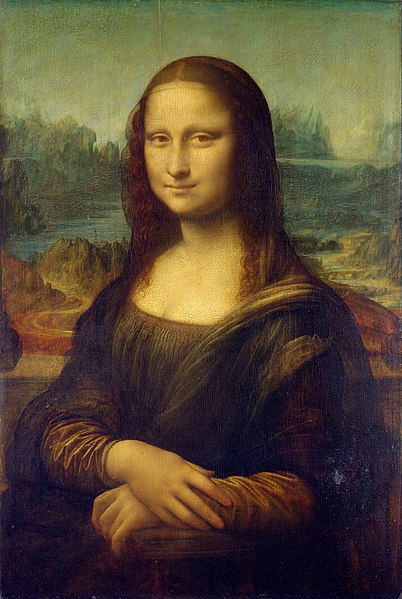
\includegraphics[width=0.45\textwidth]{monalisa}
	\caption[Mona Lisa, again]{It's Mona Lisa again. \blindtext}
	\labfig{normalmonalisa}
\end{figure}

While the format of the caption is managed by \Package{caption}, its 
position is handled by the \Package{floatrow} package. Achieving this 
result has been quite hard, but now I am pretty satisfied. In two-side 
mode, the captions are printed in the correct margin.

Tables can be inserted just as easily as figures, as exemplified by the 
following code:

\begin{lstlisting}[caption={Caption of a listing.}]
\begin{table}
\begin{tabular}{ c c c c }
	\toprule
	col1 & col2 & col3 & col 4 \\
	\midrule
	\multirow{3}{4em}{Multiple row} & cell2 & cell3 & cell4\\ &
	cell5 & cell6 & cell7 \\ &
	cell8 & cell9 & cell10 \\
	\multirow{3}{4em}{Multiple row} & cell2 & cell3 & cell4 \\ &
	cell5 & cell6 & cell7 \\ &
	cell8 & cell9 & cell10 \\
	\bottomrule
\end{tabular}
\end{table}
\end{lstlisting}

which results in the useless \vreftab{useless}.

\begin{table}[ht]
\caption[A useless table]{A useless table.}
\labtab{useless}
\begin{tabular}{ c c c c }
	\toprule
	col1 & col2 & col3 & col 4 \\
	\midrule
	\multirow{3}{4em}{Multiple row} & cell2 & cell3 & cell4\\ &
	cell5 & cell6 & cell7 \\ &
	cell8 & cell9 & cell10 \\
	\multirow{3}{4em}{Multiple row} & cell2 & cell3 & cell4 \\ &
	cell5 & cell6 & cell7 \\ &
	cell8 & cell9 & cell10 \\
	\bottomrule
\end{tabular}
\end{table}

I don't have much else to say, so I will just insert some blind text. 
\blindtext

\section{Margin Figures and Tables}

Marginfigures can be inserted with the environment 
\Environment{marginfigure}. In this case, the whole picture is confined 
to the margin and the caption is below it. \reffig{marginmonalisa} is 
obtained with something like this:

\begin{lstlisting}[caption={Another caption.}]
\begin{marginfigure}
	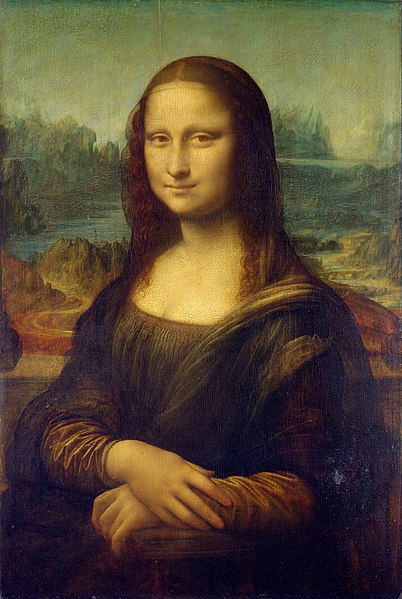
\includegraphics{monalisa}
	\caption[The Mona Lisa]{The Mona Lisa.}
	\labfig{marginmonalisa}
\end{marginfigure}
\end{lstlisting}

There is also the \Environment{margintable} environment, of which 
\reftab{anotheruseless} is an example. Notice how you can place the 
caption above the table by just placing the \Command{caption} command 
before beginning the \Environment{tabular} environment. Usually, figure 
captions are below, while table captions are above. This rule is also 
respected for normal figures and tables: the captions are always on the 
side, but for figure they are aligned to the bottom, while for tables to 
the top.

\begin{margintable}
\caption[Another useless table]{Another useless table.}
\labtab{anotheruseless}
\raggedright
\begin{tabular}{ c c c c }
	\hline
	col1 & col2 & col3 \\
	\hline
	\multirow{3}{4em}{Multiple row} & cell2 & cell3 \\ & cell5 & cell6 
	\\ & cell8 & cell9 \\ \hline
\end{tabular}
\end{margintable}

Marginfigures and tables can be positioned with an optional offset 
command, like so:

\begin{lstlisting}
\begin{marginfigure}[offset]
	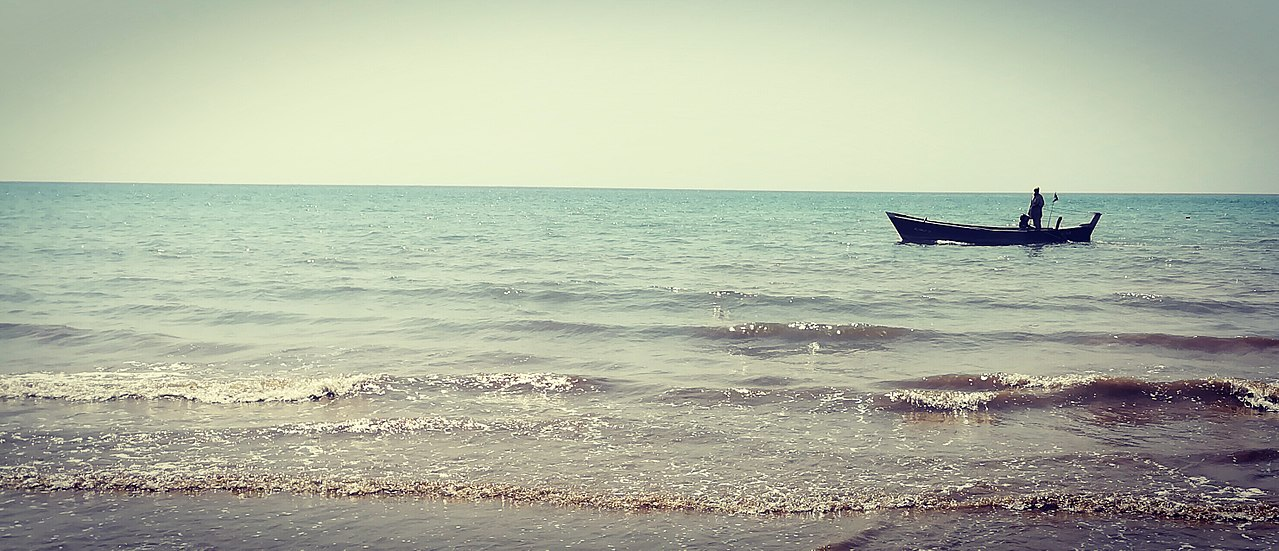
\includegraphics{seaside}
\end{marginfigure}
\end{lstlisting}

Offset ca be either a measure or a multiple of \Command{baselineskip}, 
much like with \Command{sidenote}, \Command{marginnote} and 
\Command{margintoc}.\todo{Improve this part.} If you are wondering how I 
inserted this orange bubble, have a look at the \Package{todo} package.

\section{Wide Figures and Tables}

With the environments \Environment{figure*} and \Environment{table*} you 
can insert figures which span the whole page width. For example, here 
are a wide figure and a wide table.

\begin{figure*}[h!]
	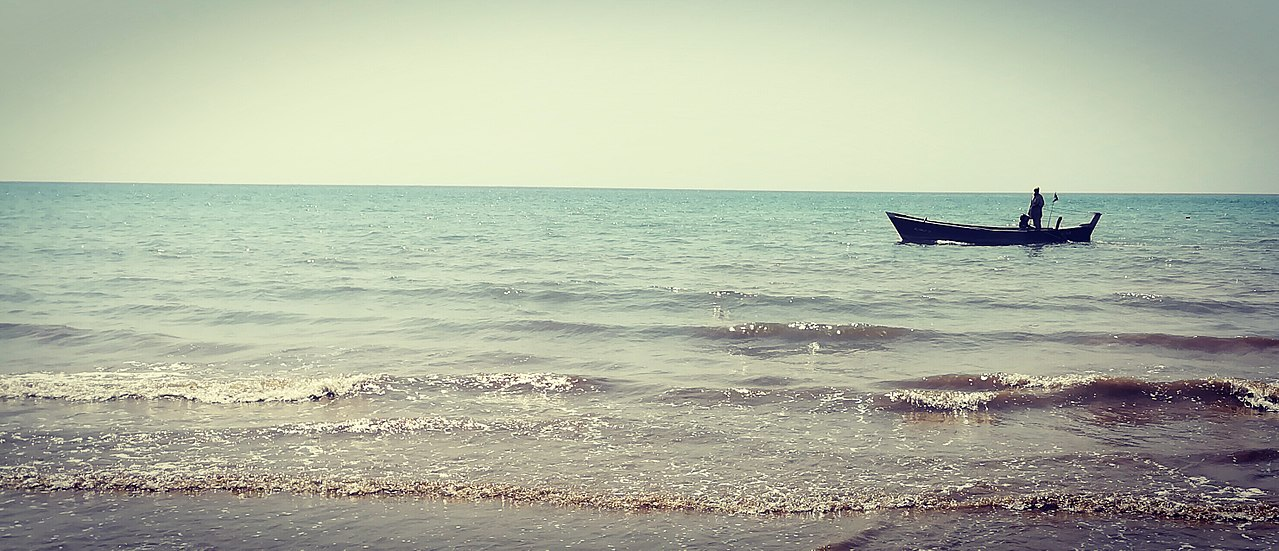
\includegraphics{seaside}
	\caption[A wide seaside]{A wide seaside, and a wide caption.
		Credits: By Bushra Feroz, CC BY-SA 4.0, \url{https://commons.wikimedia.org/w/index.php?curid=68724647}}
\end{figure*}

\begin{table*}[h!]
    \caption{A wide table with invented data about three people living in the UK. Note that wide figures and tables are centered and their caption also extends into the margin.}
    \begin{tabular}{p{2.0cm} p{2.0cm} p{2.0cm} p{2.0cm} p{2.0cm} p{2.0cm} p{1.5cm}}
        \toprule
        Name    & Surname   & Job       & Salary           & Age   & Height    & Country \\
        \midrule
        Alice   & Red       & Writer    & 4.000 \pounds    & 34    & 167 cm     & England \\
        Bob     & White     & Bartender & 2.000 \pounds    & 24    & 180 cm     & Scotland \\
        Drake   & Green     & Scientist & 4.000 \pounds    & 26    & 175 cm     & Wales \\
        \bottomrule
    \end{tabular}
\end{table*}

It is the user's responsibility to adjust the width of the table, if 
necessary, until it is aesthetically pleasing. The previous table was 
obtained with the following code:

\begin{lstlisting}[caption=How to typeset a wide table]
\begin{table*}[h!]
    \caption{A wide table with invented data about three people living in the UK. Note that wide figures and tables are centered and their caption also extends into the margin.}
    \begin{tabular}{p{2.0cm} p{2.0cm} p{2.0cm} p{2.0cm} p{2.0cm} p{2.0cm} p{1.5cm}}
        \toprule
        Name    & Surname   & Job       & Salary           & Age   & Height    & Country \\
        \midrule
        Alice   & Red       & Writer    & 4.000 \pounds    & 34    & 167 cm     & England \\
        Bob     & White     & Bartender & 2.000 \pounds    & 24    & 180 cm     & Scotland \\
        Drake   & Green     & Scientist & 4.000 \pounds    & 26    & 175 cm     & Wales \\
        \bottomrule
    \end{tabular}
\end{table*}
\end{lstlisting}

The \Package{floatrow} package provides the \enquote{H} specifier to 
instruct \LaTeX to position the figure (or table) in precisely the same 
position it occupies in the source code. However, this specifier does 
not work with wide figures or tables: you should use \enquote{h!} 
instead, like so: \lstinline|\begin{figure*}[h!]|.

You may have noticed the full width image at the very beginning of this
chapter: that, however, is set up in an entirely different way, which
you'll read about in \vrefch{layout}.

\Class{kaobook} also supports paginated tables (have a look at the 
\Package{longtable} package). The 
\Environment{longtable}\sidenote{Interestingly, \Environment{longtable}s 
may require up to four rounds of compilation before they are typeset 
correctly.} environment behaves a bit differently from 
\Environment{table}, in that \Environment{longtable} encompasses both 
\Environment{table} and \Environment{tabular}, so that you can write, 
\eg,

\begin{lstlisting}[caption=Example of a longtable]
\begin{longtable}{|l c c|}
    \hline
    One & Two & Three \\
    Left & Center & Center \\
    \hline
    \caption{Caption of the longtable.}
\end{longtable}
\end{lstlisting}

to obtain the following table:
\begin{longtable}{|l c c|}
    \hline
    One & Two & Three \\
    Left & Center & Center \\
    \hline
    \caption{Caption of the longtable.}
\end{longtable}

The caption of a \Environment{longtable} is always positioned below the 
table, and it has the same width as the text (it doesn't extend into the 
margin). However, sometimes you may need a \Environment{longtable} that 
is so wide that it trespass into the margins; in those cases, you may 
want to also increase the width of the caption. To do so, you'll have to 
write two additional commands, one before and one after the 
\Environment{longtable}:

\begin{lstlisting}[caption=Increasing the width of the caption of a \Environment{longtable}.]
\floatsetup[longtable]{margins=centering,LTcapwidth=table} % Add this line before the longtable to increase the caption width
\begin{longtable}{lp{8cm}p{5cm}p{2cm}}
...
\end{longtable}
\floatsetup[longtable]{margins=raggedright,LTcapwidth=\textwidth} % Add this line after the longtable to revert the previous change
\end{lstlisting}

Having seen figures and tables, it is now time to tackle 
hyperreferences.

% \setchapterstyle{kao}
%\setchapterpreamble[u]{\margintoc}
\chapter{References}
\labch{references}

\section{Citations}

\index{citations}
To cite someone \sidecite{Visscher2008,James2013} is very simple: just 
use the \Command{sidecite}\index{\Command{sidecite}} command. It does 
not have an offset argument yet, but it probably will in the future. 
This command supports multiple entries, as you can see, and by default 
it prints the reference on the margin as well as adding it to the 
bibliography at the end of the document. Note that the citations have 
nothing to do with the text,\sidecite{James2013} but they are completely 
random as they only serve the purpose to illustrate the feature.

For this setup I wrote a separate package, \Package{kaobiblio}, which 
you can find in the \Package{styles} directory and include in your main 
tex file. This package accepts all the options that you can pass to 
\Package{biblatex}, and actually it passes them to \Package{biblatex} 
under the hood. Moreover, it also defines some commands, like 
\Command{sidecite}, and environments that can be used within a 
\Class{kao} book.\sidenote[][-.9cm]{For this reason you should always 
use \Package{kaobiblio} instead of \Package{biblatex}, but the syntax 
and the options are exactly the same.}

If you want to use \Package{bibtex} instead of \Package{biblatex},
pass the option \Option{backend=bibtex} to \Package{kaobiblio}.
\Package{kaobiblio} also supports two options that are not shared with
\Package{biblatex}: \Option{addspace} and \Option{linkeverything},
both of which are boolean options, meaning that they can take
either \enquote{true} or \enquote{false} as a value. If you
pass \Option{addspace=true} when loading \Package{kaobiblio},
a space will be automatically added before the citation marks.
If you pass \Option{linkeverything=true}, the author's name in
the authoryear-* and authortitle-* styles will be a hyperlink
like the year.\sidenote{The fact that the author name is not
a hyperlink bothers more than one biblatex user. There are
\href{https://github.com/plk/biblatex/issues/428}{strong arguments}
\emph{against} hyperlinking the author name, but in my personal opinion, 
linking the author's name does not result in any problems in most 
practical cases.}

As you have seen, the \Command{sidecite} command will print a citation 
in the margin. However, this command would be useless without a way to 
customise the format of the citation, so the \Class{kaobook} provides 
also the \Command{formatmargincitation} command. By \enquote{renewing} 
that command, you can choose which items will be printed in the margins. 
The best way to understand how it works is to see the actual definition 
of this command.

\begin{lstlisting}[style=kaolstplain,linewidth=1.5\textwidth]
\newcommand{\formatmargincitation}[1]{%
	\parencite{#1}: \citeauthor*{#1} (\citeyear{#1}), \citetitle{#1}%
}
\end{lstlisting}

Thus, the \Command{formatmargincitation} accepts one parameter, which is 
the citation key, and prints the parencite followed by a colon, then the 
author, then the year (in brackets), and finally the 
title.\sidecite{Battle2014} Now, suppose that you wish the margin 
citation to display the year and the author, followed by the title, and 
finally a fixed arbitrary string; you would add to your document:

\begin{lstlisting}[style=kaolstplain,linewidth=1.5\textwidth]
\renewcommand{\formatmargincitation}[1]{%
	\citeyear{#1}, \citeauthor*{#1}: \citetitle{#1}; very interesting!%
}
\end{lstlisting}

\renewcommand{\formatmargincitation}[1]{%
	\citeyear{#1}, \citeauthor*{#1}: \citetitle{#1}; very interesting!%
}

The above code results in citations that look like the 
following.\sidecite{Zou2005} Of course, changing the format is most 
useful when you also change the default bibliography style. For 
instance, if you want to use the \enquote{philosophy-modern} style for 
your bibliography, you might have something like this in the preamble:

\begin{lstlisting}[style=kaolstplain,linewidth=1.5\textwidth]
\usepackage[style=philosophy-modern]{styles/kaobiblio}
\renewcommand{\formatmargincitation}[1]{%
	\sdcite{#1}%
}
\addbibresource{main.bib}
\end{lstlisting}

\renewcommand{\formatmargincitation}[1]{%
	\parencite{#1}: \citeauthor*{#1} (\citeyear{#1}), \citetitle{#1}%
}

The commands like \Command{citeyear}, \Command{parencite}
and \Command{sdcite} are just examples. A full
reference of the available commands can be found in this
\href{http://tug.ctan.org/info/biblatex-cheatsheet/biblatex-cheatsheet.pdf}{cheatsheet},
under the \enquote{Citations} section.

Finally, to compile a document containing citations, you need to use an 
external tool, which for this class is biber. You need to run the 
following (assuming that your tex file is called main.tex):

\begin{lstlisting}[style=kaolstplain]
$ pdflatex main
$ biber main
$ pdflatex main
\end{lstlisting}

\section{Glossaries and Indices}

\index{glossary}
The \Class{kaobook} class loads the packages \Package{glossaries} and 
\Package{imakeidx}, with which you can add glossaries and indices to 
your book. For instance, I previously defined some glossary entries and 
now I am going to use them, like this: \gls{computer}. 
\Package{glossaries} also allows you to use acronyms, like the 
following: this is the full version, \acrfull{fpsLabel}, and this is the 
short one \acrshort{fpsLabel}. These entries will appear in the glossary 
in the backmatter.

Unless you use \href{https://www.overleaf.com}{Overleaf} or some other 
fancy IDE for \LaTeX, you need to run an external command from your 
terminal in order to compile a document with a glossary. In particular, 
the commands required are:\sidenote{These are the commands you would run 
in a UNIX system, but see also \nrefsec{compiling}; I have no idea about 
how it works in Windows.}

\begin{lstlisting}[style=kaolstplain]
$ pdflatex main
$ makeglossaries main
$ pdflatex main
\end{lstlisting}

Note that you need not run \texttt{makeglossaries} every time you 
compile your document, but only when you change the glossary entries.

\index{index}
To create an index, you need to insert the command 
\lstinline|\index{subject}| whenever you are talking about 
\enquote{subject} in the text. For instance, at the start of this 
paragraph I would write \lstinline|index{index}|, and an entry would be 
added to the Index in the backmatter. Check it out!

\marginnote[2mm]{In theory, you would need to run an external command 
for the index as well, but luckily the package we suggested, 
	\Package{imakeidx}, can compile the index automatically.}

\index{nomenclature}
A nomenclature is just a special kind of index; you can find one at the end of
this book. To insert a nomenclature, we use the package \Package{nomencl} and
add the terms with the command \Command{nomenclature}. We put then a
\Command{printnomenclature} where we want it to appear.

Also with this package we need to run an external command to compile the 
document, otherwise the nomenclature will not appear:

\begin{lstlisting}[style=kaolstplain]
$ pdflatex main
$ makeindex main.nlo -s nomencl.ist -o main.nls
$ pdflatex main
\end{lstlisting}

These packages are all loaded in 
\href{style/packages.sty}{packages.sty}, one of the files that come with 
this class. However, the configuration of the elements is best done in 
the main.tex file, since each book will have different entries and 
styles.

Note that the \Package{nomencl} package caused problems when the 
document was compiled, so, to make a long story short, I had to prevent 
\Package{scrhack} to load the hack-file for \Package{nomencl}. When 
compiling the document on Overleaf, however, this problem seem to 
vanish.

\marginnote[-19mm]{This brief section was by no means a complete 
reference on the subject, therefore you should consult the documentation 
of the above package to gain a full understanding of how they work.}

\section{Hyperreferences}
\labsec{hyprefs}

\index{hyperreferences}
Together with this class we provide a handy package to help you 
referencing the same elements always in the same way, for consistency 
across the book. First, you can label each element with a specific 
command. For instance, should you want to label a chapter, you would put 
\lstinline|\labch{chapter-title}| right after the \Command{chapter} 
directive. This is just a convenience, because \Command{labch} is
actually just an alias to \lstinline|\label{ch:chapter-title}|, so it 
spares you the writing of \enquote{ch:}. We defined similar commands for 
many typically labeled elements, including:

\begin{multicols}{2}
\setlength{\columnseprule}{0pt}
\begin{itemize}
	\item Page: \Command{labpage}
	\item Part: \Command{labpart}
	\item Chapter: \Command{labch}
	\item Section: \Command{labsec}
	\item Figure: \Command{labfig}
	\item Table: \Command{labtab}
	\item Definition: \Command{labdef}
	\item Assumption: \Command{labassum}
	\item Theorem: \Command{labthm}
	\item Proposition: \Command{labprop}
	\item Lemma: \Command{lablemma}
	\item Remark: \Command{labremark}
	\item Example: \Command{labexample}
	\item Exercise: \Command{labexercise}
\end{itemize}
\end{multicols}

Of course, we have similar commands for referencing those elements. 
However, since the style of the reference should depend on the context, 
we provide different commands to reference the same thing. For instance, 
in some occasions you may want to reference the chapter by name, but 
other times you want to reference it only by number. In general, there 
are four reference style, which we call plain, vario, name, and full.

The plain style references only by number. It is accessed, for chapters, 
with \lstinline|\refch{chapter-title}| (for other elements, the syntax 
is analogous). Such a reference results in: \refch{references}.

The vario and name styles rest upon the \Package{varioref} package. 
Their syntax is \lstinline|\vrefch{chapter-title}| and 
\lstinline|\nrefch{chapter-title}|, and they result in: 
\vrefch{references}, for the vario style, and: \nrefch{references}, for 
the name style. As you can see, the page is referenced in 
\Package{varioref} style.

The full style references everything. You can use it with 
\lstinline|\frefch{chapter-title}| and it looks like this: 
\frefch{references}.

Of course, all the other elements have similar commands (\eg for parts 
you would use \lstinline|\vrefpart{part-title}| or something like that). 
However, not all elements implement all the four styles. The commands 
provided should be enough, but if you want to see what is available or 
to add the missing ones, have a look at the 
\href{styles/kaorefs.sty}{attached package}.

In order to have access to all these features, the \Package{kaorefs} 
should be loaded in the preamble of your document. It should be loaded 
last, or at least after \Package{babel} (or \Package{polyglossia}) and 
\Package{plaintheorems} (or \Package{mdftheorems}). Options can be 
passed to it like to any other package; in particular, it is possible to 
specify the language of the captions. For instance, if you specify 
\enquote{italian} as an option, instead of \enquote{Chapter} it will be 
printed \enquote{Capitolo}, the Italian analog. If you know other 
languages, you are welcome to contribute the translations of these 
captions! Feel free to contact the author of the class for further 
details. 

The \Package{kaorefs} package also include \Package{cleveref}, so it is 
possible to use \Command{cref} in addition to all the previously 
described referencing commands.

\section{A Final Note on Compilation}
\labsec{compiling}

Probably the easiest way to compile a latex document is with the 
\Package{latexmk} script, as it can take care of everything, if properly 
configured, from the bibliography to the glossary. The command to issue, 
in general, is:

\begin{lstlisting}
latexmk [latexmk_options] [filename ...]
\end{lstlisting}

\Package{latexmk} can be extensively configured (see
\url{https://mg.readthedocs.io/latexmk.html}). For convenience, I print 
here an example configuration that would cover all the steps described 
above.

\begin{lstlisting}
# By default compile only the file called 'main.tex'
@default_files = ('main.tex');

# Compile the glossary and acronyms list (package 'glossaries')
add_cus_dep( 'acn', 'acr', 0, 'makeglossaries' );
add_cus_dep( 'glo', 'gls', 0, 'makeglossaries' );
$clean_ext .= " acr acn alg glo gls glg";
sub makeglossaries {
   my ($base_name, $path) = fileparse( $_[0] );
   pushd $path;
   my $return = system "makeglossaries", $base_name;
   popd;
   return $return;
}

# Compile the nomenclature (package 'nomencl')
add_cus_dep( 'nlo', 'nls', 0, 'makenlo2nls' );
sub makenlo2nls {
    system( "makeindex -s nomencl.ist -o \"$_[0].nls\" \"$_[0].nlo\"" );
}
\end{lstlisting}

However, if you'd rather not use an external package and want to do 
everything manually, here are some tips.\sidenote{As the author only 
uses Linux and compiles everything from the command line, he doesn't 
know how the compilation works in Windows or Mac. The tips, therefore, 
refer to the usage with Linux from the command line.}

\minisec{Compiling the examples in the kaobook repository}
To compile the examples, and in particular the documentation, that are 
in the \Path{examples} directory of the 
\href{https://github.com/fmarotta/kaobook}{kaobook repository} on 
GitHub, do as follows. \lstinline[language=bash]|cd| into the root 
directory of the repository, and run
\lstinline|pdflatex -output-directory examples/documentation main.tex|. 
With this trick, you can compile the documentation using the class files 
pertaining to the repository (and not, say, those in your texmf tree). 
The \enquote{-output-directory} option works with the other 
\LaTeX-related commands such as biber and makeglossaries.

A note of warning: sometimes \LaTeX\ needs more than one run to get the
correct position of each element; this is true in particular for the
positioning of floating elements like figures, tables, and margin notes.
Occasionally, \LaTeX\ can need up to four re-runs, so If the alignment
of margin elements looks odd, or if they bleed into ther main text, try
running pdflatex one more time.

% 
% \pagelayout{wide} % No margins
% \addpart{Design and Additional Features}
% \pagelayout{margin} % Restore margins
% 
% \setchapterimage[6cm]{seaside}
\setchapterpreamble[u]{\margintoc}
\chapter{Page Design}
\labch{layout}

\section{Headings}

So far, in this document I used two different styles for the chapter
headings: one has the chapter name, a rule and, in the margin, the
chapter number; the other has an image at the top of the page, and
the chapter title is printed in a box (like for this chapter). There
is one additional style, which I used only in the \nrefch{appendix};
there, the chapter title is enclosed in two horizontal rules, and
the chapter number (or letter, in the case of the appendix) is above
it.\sidenote[][.7cm]{To be honest, I do not think that mixing heading
styles like this is a wise choice, but in this document I did it only to
show you how they look.}

Every book is unique, so it makes sense to have different styles from 
which to choose. Actually, it would be awesome if whenever a 
\Class{kao}-user designs a new heading style, he or she added it to the 
three styles already present, so that it will be available for new users 
and new books.

The choice of the style is made simple by the \Command{setchapterstyle} 
command. It accepts one option, the name of the style, which can be: 
\enquote{plain}, \enquote{kao}, \enquote{bar}, or 
\enquote{lines}.\sidenote{Plain is the default \LaTeX\xspace title 
style; the other ones are self explanatory.} If instead you want the 
image style, you have to use the command \Command{setchapterimage}, 
which accepts the path to the image as argument; you can also provide an 
optional parameter in square brackets to specify the height of the 
image. \Command{setchapterimage} automatically sets the chapter style to 
\enquote{bar} for that chapter (and also for subsequent chapters).

Let us make some examples. In this book, I begin a normal chapter with 
the lines:
\begin{lstlisting}
\setchapterstyle{kao}
\setchapterpreamble[u]{\margintoc}
\chapter{Title of the Chapter}
\labch{title}
\end{lstlisting}

In Line 1 I choose the style for the title to be \enquote{kao}. Then, I 
specify that I want the margin toc. The rest is ordinary administration 
in \LaTeX, except that I use my own \Command{labch} to label the 
chapter. Actually, the \Command{setchapterpreamble} is a standard 
\KOMAScript\xspace one, so I invite you to read about it in the KOMA
documentation. Once the chapter style is set, it holds until you change 
it.\sidenote{The \Command{margintoc} has to be specified at every 
chapter. Perhaps in the future this may change; it all depends on how 
this feature will be welcomed by the users, so keep in touch with me if 
you have preferences!} Whenever I want to start a chapter with an image, 
I simply write:

\begin{lstlisting}
\setchapterimage[7cm]{path/to/image.png} % Optionally specify the height
\setchapterpreamble[u]{\margintoc}
\chapter{Catchy Title} % No need to set a chapter style
\labch{catchy}
\end{lstlisting}

If you prefer, you can also specify the style at the beginning of the 
main document, and that style will hold until you change it again.

\section{Headers \& Footers}

Headers and footers in \KOMAScript\xspace are handled by the 
\Package{scrlayer-scrpage} package. There are two basic style: 
\enquote{scrheadings} and \enquote{plain.scrheadings}. The former is 
used for normal pages, whereas the latter is used in title pages (those 
where a new chapter starts, for instance) and, at least in this book, in 
the front matter. At any rate, the style can be changed with the 
\Command{pagestyle} command, \eg 
\lstinline|\pagestyle{plain.scrheadings}|.

In both styles, the footer is completely empty. In plain.scrheadings,
also the header is absent (otherwise it wouldn't be so plain\ldots), but 
in the normal style the design is reminiscent of the \enquote{kao} style
for chapter titles.

\section{\Option{twoside} mode}

\begin{kaobox}[title=To Do]
The \Option{twoside} class option is still unstable and may lead to 
unexpected behaviours. Great strides have been done since the first 
version of \Class{kaobook}, but some work still needs to be done. As 
always, any help will be greatly appreciated.
\end{kaobox}

By passing the \Option{twoside} option to the \Class{kaobook}, the
style of left and right pages will be different, similarly to a
printed book. In digital books, having a symmetrical layout for
left and right pages is less important, and you may be tempted
to use the \Option{twoside=false} option. However, keep in mind
that in \enquote{oneside} mode the \Command{uppertitleback} and
\Command{lowertitleback} commands are not available.\sidenote{Another
useful thing to keep in mind is that, when \Option{twoside=true}, an
extra white page will be added to the frontmatter.} If you want to have 
the upper/lower titleback in a one-side document, just add manually the 
contents that you'd put using the upper/lower titleback commands.

\section{Table of Contents}

Another important part of a book is the table of contents. By default, 
in \Class{kaobook} there is an entry for everything: list of figures, 
list of tables, bibliographies, and even the table of contents itself. 
Not everybody might like this, so we will provide a description of the 
changes you need to do in order to enable or disable each of these 
entries. In the following \reftab{tocentries}, each item corresponds to 
a possible entry in the \acrshort{tocLabel}, and its description is the 
command you need to provide to have such entry. These commands are 
specified in the attached \href{style/style.sty}{style 
package},\sidenote{In the same file, you can also choose the titles of 
these entries.} so if you don't want the entries, just comment the 
corresponding lines.

Of course, some packages, like those for glossaries and indices, will 
try to add their own entries.\marginnote{In a later section, we will see 
how you can define your own floating environment, and endow it with an 
entry in the \acrshort{tocLabel}.} In such cases, you have to follow the 
instructions specific to that package. Here, since we have talked about 
glossaries and notations in \refch{references}, we will briefly see how
to configure them.

\begin{table}
\footnotesize
\caption{Commands to add a particular entry to the table of contents.}
\labtab{tocentries}
\begin{tabular}{ l@{\hspace{1mm}}l }
	\toprule
	Entry & Command to Activate \\
	\midrule
	Table of Contents & \lstinline|\setuptoc{toc}{totoc}| \\
    List of Figs/Tabs & \lstinline|\PassOptionsToClass{toc=listof}{\@baseclass}| \\
	Bibliography & \lstinline|\PassOptionsToClass{toc=bibliography}{\@baseclass}| \\
	\bottomrule
\end{tabular}
\end{table}

For the \Package{glossaries} package, use the \enquote{toc} option when 
you load it: \lstinline|\usepackage[toc]{glossaries}|. For 
\Package{nomencl}, pass the \enquote{intoc} option at the moment of 
loading the package. Both \Package{glossaries} and \Package{nomencl} are 
loaded in the attached \href{style/packages.sty}{\enquote{packages} 
package}.

Additional configuration of the table of contents can be performed 
through the packages \Package{etoc}, which is loaded because it is 
needed for the margintocs, or the more traditional \Package{tocbase}. 
Read the respective documentations if you want to be able to change the 
default \acrshort{tocLabel} style.\sidenote[][*-1]{(And please, send me 
a copy of what you have done, I'm so curious!)}

\section{Paper Size}

Recent versions of Kaobook support paper sizes different from the
default A4. It is possible to pass the name of the paper as an option
to the class, as we are accustomed for any other \LaTeX\ class. For
example, the class option \Option{b5paper} would set the paper size
to the B5 format.

We also support the paper sizes specified in
\href{https://www.bod.de/hilfe/hilfe-und-service.html?cmd=SINGLE\&entryID=2494\_GER\_WSS\&eo=2\&title=welche-buchformate-gibt-es}{this
web page} and some additional sizes requested by the users, with the 
option names specified in \reftab{papersizes}.

\begin{margintable}[*-6]
	\caption{Some non-standard paper sizes supported by kaobook.}
	\labtab{papersizes}
	\begin{tabular}{ll}
		\toprule
		Dimension & Option name \\
		\midrule
		12.0cm x 19.0cm & smallpocketpaper \\
		13.5cm x 21.5cm & pocketpaper \\
		14.8cm x 21.0cm & a5paper \\
		15.5cm x 22.0cm & juvenilepaper \\
		17.0cm x 17.0cm & smallphotopaper \\
		21.0cm x 15.0cm & appendixpaper \\
		17.0cm x 22.0cm & cookpaper \\
		19.0cm x 27.0cm & illustratedpaper \\
		17.0cm x 17.0cm & photopaper \\
		16.0cm x 24.0cm & f24paper \\
		%21.0cm x 29.7cm & a4paper \\
		\bottomrule
	\end{tabular}
\end{margintable}

For instance, to use the \enquote{smallpocketpaper} add the correct 
description at the beginning of the documentclass instruction:
\begin{lstlisting}
\documentclass[
		smallpocketpaper,
		fontsize=10pt,
		twoside=false,
		%open=any,
		secnumdepth=1,
]{kaobook}
\end{lstlisting}

Sometimes it is convenient to adopt a landscape view; \Class{kaobook} 
provides two additional options, \Option{a4paperlandscape} and 
\Option{169paperlandscape}, which set the page in landscape mode with 
width-to-height ratios of, respectively, 1.414 and 16:9.

\section{Page Layout}

Besides the page style, you can also change the width of the content of 
a page. This is particularly useful for pages dedicated to part titles, 
where having the 1.5-column layout might be a little awkward, or for 
pages where you only put figures, where it is important to exploit all 
the available space.

In practice, there are two layouts: \enquote{wide} and \enquote{margin}. 
The former suppresses the margins and allocates the full page for 
contents, while the latter is the layout used in most of the pages of 
this book, including this one. The wide layout is also used 
automatically in the front and back matters.

\marginnote{Sometimes it is desirable to increase the width for just one 
or a few paragraphs; the \Environment{widepar} environment does that: 
wrap your paragraphs in this environment, and they will occupy the full 
width of the page.}

To change page layout, use the \Command{pagelayout} command. For 
example, when I start a new part, I write:

\begin{lstlisting}
\pagelayout{wide}
\addpart{Title of the New Part}
\pagelayout{margin}
\end{lstlisting}

Beyond these two basic layouts, it is also possible to finely tune the 
page layout by redefining the \Command{marginlayout} command. This 
command is called internally by the higher-level \Command{pagelayout}, 
and it is responsible for setting the width of the margins and of the 
text. The default definition is:

\begin{lstlisting}
\newcommand{\marginlayout}{%
	\newgeometry{
		top=27.4mm,				% height of the top margin
		bottom=27.4mm,			% height of the bottom margin
		inner=24.8mm,			% width of the inner margin
		textwidth=107mm,		% width of the text
		marginparsep=8.2mm,		% width between text and margin
		marginparwidth=49.4mm,	% width of the margin
	}%
}
\end{lstlisting}

so if you want to, say, decrease the width of the margin while 
increasing the width of the text, you could write in the preamble of 
your document something like:

\begin{lstlisting}
\renewcommand{\marginlayout}{%
	\newgeometry{
		top=27.4mm,				% height of the top margin
		bottom=27.4mm,			% height of the bottom margin
		inner=24.8mm,			% width of the inner margin
		textwidth=117mm,		% width of the text
		marginparsep=8.2mm,		% width between text and margin
		marginparwidth=39.4mm,	% width of the margin
	}%
}
\end{lstlisting}

where the text width has been increased by 10mm and the margin width has 
been decreased by 10mm.

\section{Numbers \& Counters}

In this short section we shall see how dispositions, sidenotes and 
figures are numbered in the \Class{kaobook} class.

By default, dispositions are numbered up to the section in \Class{kaobook}
and up to the subsection in \Class{kaohandt}. This can be changed by
passing the option \Option{secnumdepth} to\Class{kaobook} or
\Class{kaohandt} (e.g. 1 corresponds to section and 2 corresponds to
subsections).

The sidenotes counter is the same across all the document, but if you 
want it to reset at each chapter, just uncomment the line

\begin{lstlisting}[style=kaolstplain]
\counterwithin*{sidenote}{chapter}
\end{lstlisting}

in the \Package{styles/style.sty} package provided by this class.

Figure and Table numbering is also per-chapter; to change that, use 
something like:

\begin{lstlisting}[style=kaolstplain]
\renewcommand{\thefigure}{\arabic{section}.\arabic{figure}}
\end{lstlisting}

\section{White Space}

One of the things that I find most hard in \LaTeX\xspace is to finely 
tune the white space around objects. There are not fixed rules, each 
object needs its own adjustment. Here we shall see how some spaces are 
defined at the moment in this class.\marginnote{Attention! This section 
may be incomplete.}

\textbf{Space around sidenotes and citations marks}

There should be no space before or after sidenotes and citation marks, 
like so:

sidenote\sidenote{This paragraph can be used to diagnose any problems:
if you see whitespace around sidenotes or citation marks, probably
a \% sign is missing somewhere in the definitions of the class
macros.}sidenote\newline
citation\cite{James2013}citation

\textbf{Space around figures and tables}

\begin{lstlisting}[style=kaolstplain]
\renewcommand\FBaskip{.4\topskip}
\renewcommand\FBbskip{\FBaskip}
\end{lstlisting}

\textbf{Space around captions}

\begin{lstlisting}[style=kaolstplain]
\captionsetup{
	aboveskip=6pt,
	belowskip=6pt
}
\end{lstlisting}

\textbf{Space around displays (\eg equations)}

\begin{lstlisting}[style=kaolstplain]
\setlength\abovedisplayskip{6pt plus 2pt minus 4pt}
\setlength\belowdisplayskip{6pt plus 2pt minus 4pt}
\abovedisplayskip 10\p@ \@plus2\p@ \@minus5\p@
\abovedisplayshortskip \z@ \@plus3\p@
\belowdisplayskip \abovedisplayskip
\belowdisplayshortskip 6\p@ \@plus3\p@ \@minus3\p@
\end{lstlisting}

% \setchapterstyle{kao}
\setchapterpreamble[u]{\margintoc}
\chapter{Mathematics and Boxes}
\labch{mathematics}

\section{Theorems}

Despite most people complain at the sight of a book full of equations, 
mathematics is an important part of many books. Here, we shall 
illustrate some of the possibilities. We believe that theorems, 
definitions, remarks and examples should be emphasised with a shaded 
background; however, the colour should not be to heavy on the eyes, so 
we have chosen a sort of light yellow.\sidenote{The boxes are all of the 
same colour here, because we did not want our document to look like 
\href{https://en.wikipedia.org/wiki/Harlequin}{Harlequin}.}

\begin{definition}
\labdef{openset}
Let $(X, d)$ be a metric space. A subset $U \subset X$ is an open set 
if, for any $x \in U$ there exists $r > 0$ such that $B(x, r) \subset 
U$. We call the topology associated to d the set $\tau\textsubscript{d}$ 
of all the open subsets of $(X, d).$
\end{definition}

\refdef{openset} is very important. I am not joking, but I have inserted 
this phrase only to show how to reference definitions. The following 
statement is repeated over and over in different environments.

\begin{theorem}
A finite intersection of open sets of (X, d) is an open set of (X, d), 
i.e $\tau\textsubscript{d}$ is closed under finite intersections. Any 
union of open sets of (X, d) is an open set of (X, d).
\end{theorem}

\begin{proposition}
A finite intersection of open sets of (X, d) is an open set of (X, d), 
i.e $\tau\textsubscript{d}$ is closed under finite intersections. Any 
union of open sets of (X, d) is an open set of (X, d).
\end{proposition}

\marginnote{You can even insert footnotes inside the theorem 
environments; they will be displayed at the bottom of the box.}

\begin{lemma}
A finite intersection\footnote{I'm a footnote} of open sets of (X, d) is 
an open set of (X, d), i.e $\tau\textsubscript{d}$ is closed under 
finite intersections. Any union of open sets of (X, d) is an open set of 
(X, d).
\end{lemma}

You can safely ignore the content of the theorems\ldots I assume that if 
you are interested in having theorems in your book, you already know 
something about the classical way to add them. These example should just 
showcase all the things you can do within this class.

\begin{corollary}[Finite Intersection, Countable Union]
A finite intersection of open sets of (X, d) is an open set of (X, d), 
i.e $\tau\textsubscript{d}$ is closed under finite intersections. Any 
union of open sets of (X, d) is an open set of (X, d).
\end{corollary}

\begin{proof}
The proof is left to the reader as a trivial exercise. Hint: \blindtext
\end{proof}

\begin{definition}
Let $(X, d)$ be a metric space. A subset $U \subset X$ is an open set 
if, for any $x \in U$ there exists $r > 0$ such that $B(x, r) \subset 
U$. We call the topology associated to d the set $\tau\textsubscript{d}$ 
of all the open subsets of $(X, d).$
\end{definition}

\marginnote{
	Here is a random equation, just because we can:
	\begin{equation*}
  x = a_0 + \cfrac{1}{a_1
          + \cfrac{1}{a_2
          + \cfrac{1}{a_3 + \cfrac{1}{a_4} } } }
	\end{equation*}
}

\begin{example}
Let $(X, d)$ be a metric space. A subset $U \subset X$ is an open set 
if, for any $x \in U$ there exists $r > 0$ such that $B(x, r) \subset 
U$. We call the topology associated to d the set $\tau\textsubscript{d}$ 
of all the open subsets of $(X, d).$
\end{example}

\begin{remark}
Let $(X, d)$ be a metric space. A subset $U \subset X$ is an open set 
if, for any $x \in U$ there exists $r > 0$ such that $B(x, r) \subset 
U$. We call the topology associated to d the set $\tau\textsubscript{d}$ 
of all the open subsets of $(X, d).$
\end{remark}

As you may have noticed, definitions, example and remarks have 
independent counters; theorems, propositions, lemmas and corollaries 
share the same counter.

\begin{remark}
Here is how an integral looks like inline: $\int_{a}^{b} x^2 dx$, and 
here is the same integral displayed in its own paragraph:
\[\int_{a}^{b} x^2 dx\]
\end{remark}

There is also an environment for exercises.

\begin{exercise}
Prove (or disprove) the Riemann hypothesis.
\end{exercise}

We provide one package for the theorem styles: 
\href{kaotheorems.sty}{kaotheorems.sty}, to which you can pass the 
\Option{framed} option you do want coloured boxes around theorems, like 
in this document.\sidenote{The styles without \Option{framed} are not 
showed, but actually the only difference is that they don't have the 
yellow boxes.} You may want to edit this files according to your taste 
and the general style of the book. However, there is an option to 
customise the background colour of the boxes if you use the 
\Option{framed} option: when you load this package, you can pass it the 
\Option{background=mycolour} option (replace \enquote{mycolour} with the 
actual colour, for instance, \enquote{red!35!white}). This will change 
the colour of all the boxes, but it is also possible to override the 
default colour only for some elements. For instance, the 
\Option{propositionbackground=mycolour} option will change the colour 
for propositions only. There are similar options for theorem, 
definition, lemma, corollary, remark, and example.

\section[Boxes \& Environments]{Boxes \& Custom Environments
\sidenote[][*1.8]{Notice that in the table of contents and in the 
	header, the name of this section is \enquote{Boxes \& Environments}; 
	we achieved this with the optional argument of the \texttt{section} 
	command.}}

Say you want to insert a special section, an optional content or just 
something you want to emphasise. We think that nothing works better than 
a box in these cases. We used \Package{mdframed} to construct the ones 
shown below. You can create and modify such environments by editing the 
provided file \href{kao.sty}{kao.sty}.

\begin{kaobox}[title=Title of the box]
\blindtext
\end{kaobox}

If you set up a counter, you can even create your own numbered 
environment.

\begin{kaocounter}
	\blindtext
\end{kaocounter}

\section{Experiments}

It is possible to wrap marginnotes inside boxes, too. Audacious readers 
are encouraged to try their own experiments and let me know the 
outcomes.

\marginnote[-2.2cm]{
	\begin{kaobox}[title=title of margin note]
		Margin note inside a kaobox.\\
		(Actually, kaobox inside a marginnote!)
	\end{kaobox}
}

I believe that many other special things are possible with the 
\Class{kaobook} class. During its development, I struggled to keep it as 
flexible as possible, so that new features could be added without too 
great an effort. Therefore, I hope that you can find the optimal way to 
express yourselves in writing a book, report or thesis with this class, 
and I am eager to see the outcomes of any experiment that you may try.

%\begin{margintable}
	%\captionsetup{type=table,position=above}
	%\begin{kaobox}
		%\caption{caption}
		%\begin{tabular}{ |c|c|c|c| }
			%\hline
			%col1 & col2 & col3 \\
			%\hline
			%\multirow{3}{4em}{Multiple row} & cell2 & cell3 \\ & cell5 
			%%& cell6 \\ 
			%& cell8 & cell9 \\
			%\hline
		%\end{tabular}
	%\end{kaobox}
%\end{margintable}


\pagelayout{wide} % No margins
\addpart{A Flexible \python Tool For Fourier-Transform Noise Spectroscopy}\label{part:spectrometer}
\pagelayout{margin} % Restore margins

% mainfile: ../../main.tex
\chapter{Introduction}\label{ch:speck:introduction}

\begin{partcontribs}
    \Thispart has benefited from discussions with several people as part of a course taught during the winter semester of 2022/23~\sidecite{Bluhm2022}.
    The software package presented here was developed by me and has received contributions from Simon Humpohl,\sidenote[a]{\RWTHFZJ}
    Max Beer,\sidenotemark[a] Paul Surrey,\sidenotemark[a] and René Otten.\sidenote[b]{Then at \RWTHFZJ}
\end{partcontribs}

\AutoLettrine{Noise} is ubiquitous in condensed matter physics experiments, and in mesoscopic systems in particular it can easily drown out the sought-after signal.
In solid-state quantum technology research, devices on the length scale of the Fermi wavelength -- say tens of nanometers -- are embedded in a crystalline matrix of \num{e23} atoms.
These devices host single quantum objects such as electrons or quasiparticles---collective many-body excitations.
They are controlled and measured by classical signals routed to the device through macroscopic connections like cables and fibers.
The signals, in turn, are generated and analyzed by electronic (\eg, transistors) or optical instruments (\eg, lasers) that, in all likelihood, are again based on solid-state technology driven by the first quantum revolution~\cite{Dowling2003,Aspect2024}.
Ultimately, then, the experiments take place in an environment full of external influences from trams passing by, shaking the ground, to cosmic rays creating electron-hole or breaking up Cooper pairs.

All of these different layers to such experiments are inherently -- and in fact often fundamentally\sidenote{
    Consider Johnson-Nyquist noise in a resistor, for example.
}
-- \emph{noisy}, and it is the physicist's challenge to measure their desired effects in spite of this noise.
A well-thought-out experimental setup is hence one that has been designed taking the various noise sources into consideration, and state-of-the-art experiments often need to push the frontier in order to be successful.
From material choice in the sample to the signal path and the specs of the measurement equipment, many aspects need to be optimized and, in particular, characterized in order to assess the noise.
Indeed, the assessment of noise might even be the entire \emph{goal} of the experiment, for instance to evaluate material properties.
In this case, the quantity being measured might not be the same quantity whose noise one is interested in but rather some function of it, and the resulting data still needs to be transformed before one is able to make any practical statements about those properties.

Noise, in the sense that we are concerned with in \thethesis,\sidenote{
    Quantum noise does not fall under this scope as it may -- disregarding vacuum fluctuations for the sake of argument -- be considered \emph{emergent}; it arises from a system entangled with a (not necessarily large) number of quantum degrees of freedom being observed, \ie, tracing out the environment's degrees of freedom.
    Our lack of knowledge about this environment then appears as noise in our observations.
    See \citer{Clerk2010} for a comprehensive review of the quantum case.
}
is a stochastic process, meaning that we cannot predict with certainty a dynamical system's time evolution; it \emph{fluctuates} randomly around its noise-free value.\sidenote{
    Quantum measurements are also noisy in this sense as we cannot predict the outcome of a single-shot measurement, but here the stochasticity is in the outcomes of an ensemble rather than the sequence of values in time.
    The two are, however, closely related through ergodicity, which we will require in \cref{sec:speck:theory:time_series_estimation}.
}
Only by obtaining statistics, \ie, repeated observations, either by preparing the system in the same initial state or measuring for a certain amount of time, can we make any statements about the underlying stochastic process.
Two questions are key to assessing these statistics: first, what is the amplitude of the fluctuations?
And second, at which frequency do the fluctuations occur?
If the amplitude is small enough, we might not need to care, and if the frequency is large enough, we might be able to average out the fluctuations while if it is small enough, it might appear \emph{quasistatic} and we might be able to subtract them.
Although numerous other techniques for measuring and estimating a noise's properties exist, analyzing noise in frequency space by means of the Fourier transform imposes itself when considering these two notions.

This approach is the central topic of \thispart.
However, we will neither be too much concerned with the theoretical side of the subject matter nor with the details of its practical application in identifying and mitigating noise.\sidenote{
    I refer the interested reader to the lecture material of \citerr{Bluhm2021}{Bluhm2022} and references therein.
}
Rather, I will focus on making these techniques readily and easily accessible to experimentalists in the lab.
Given the arguments laid out above, noise spectroscopy should be an essential item in an experimentalists toolbelt.
In practice, though, we are faced with several challenges.
First, different experiments require different \gls{daq} hardware, all of which have both varying capabilities and software interfaces.
Hence, transferring a spectroscopy code from one device or setup to another is a non-trivial task and can inhibit adoption of the technique.
Albeit some instruments come with built-in spectroscopy solutions, they vary in functionality and are not easily transferred to different systems.
Second, while probably everyone finding themselves in the situation is capable of computing the noise spectrum when presented with a set of time series data, inferring the correct parameters for \acrlong{daq} given the desired parameters of the resulting spectrum can, while not difficult, be cumbersome to do.\sidenote{
    Although it is of course a good exercise, and, as a physicist, one should always strive to understand the tools one is using and the underlying principles at work.
    \Thispart is intended to provide a starting point for that.
}
Lastly, noise spectroscopy is most effective when proper visualization tools are employed.
Again, this is not a difficult task per se, but such things always incur overhead costs that can deter users from employing these essential techniques.

Here, I address these points by introducing a \python software package, \pyspeck~\cite{Hangleiter_pyspeck}, that tackles the entire processing chain of practical noise spectroscopy in a physics laboratory.
By abstracting \gls{daq} hardware into a unified interface, it is portable between different setups.
With the goal to make noise spectroscopy as accessible as possible and lower the entry barrier, it automatically handles parameter inference and hardware constraints.
Finally, it provides a comprehensive plotting solution that allows for interactively analyzing the data using various different data visualization methods.
I will employ the tool to perform displacement noise spectroscopy in a cryogenic confocal microscope in \cref{part:setup} using two different methods that highlight its versatility.

The remainder of this part is structured as follows.
In \cref{ch:speck:theory}, I review the mathematical groundwork underpinning noise spectroscopy by means of Fourier transforms of time series and discuss parameters and properties of the central quantity of interest, the \gls{psd}.
In \cref{ch:speck:software}, I then present the software package by going over its design choices and giving a walkthrough of its features using a typical workflow as an example.
I conclude by giving an outlook on future directions in \cref{ch:speck:conclusion}.

% mainfile: ../../main.tex
\chapter{Theory of spectral noise estimation}\label{ch:speck:theory}
\AutoLettrine{There} exist various methods for estimating the properties of noise in a classical signal $x(t)$.\sidenote{
    We discuss only classical noise here, meaning $x(t)$ commutes with itself at all times. For descriptions of and spectroscopy protocols for quantum noise refer to \citerr{Clerk2010}{Paz-Silva2017}, for example.
}
A simple metric quantifying the average noise amplitude of the signal observed from time $t=0$ to $t=T$ is the \gls{rms}~\cite{RMSMathworld},
\begin{align}\label{eq:speck:rms:timedomain}
    \rms_x = \sqrt{\frac{1}{T}\int_{0}^{T}\dd{t}\abs{x(t)}^2}.
\end{align}
While this already tells us \emph{something} about the noise, it is evident that a single number does not provide many clues if we were to attempt to mitigate the noise or say something qualitative about it beyond \enquote{small} and \enquote{large}.
In cases such as these, physics has often turned to the \emph{spectral} representation of the function of interest.
Knowing the frequency content of a function gives access to a wealth of information about the underlying contributing processes.
But how can we learn how a system behaves as a function of frequency?

\begin{marginfigure}[*-6]
    \centering
    \begin{circuitikz}[every node/.style={font=\sffamily\small}]
    % Draw the lock-in amplifier block
%    \node[draw, minimum width=1cm, minimum height=0.5cm, align=center] (lockin) at (0,1) {\acrshort{lia}};
    \node[draw, minimum width=1cm, minimum height=0.5cm, align=center] (lockin) at (-1,0) {\acrshort{lia}};

    % Draw the DUT (device under test)
%    \node[draw, minimum width=1cm, minimum height=0.5cm, align=center] (dut) at (0,-1) {\acrshort{dut}};
    \node[draw, minimum width=1cm, minimum height=0.5cm, align=center] (dut) at (1,0) {\acrshort{dut}};

    % Connection: Lock-In output --> DUT input
%    \draw[->, thick] (lockin.south west) to[bend right=45] node[midway, sloped, below] {$V(t)$} (dut.north west);
    \draw[->, thick] (lockin.north) to[bend left=60] node[midway, sloped, above] {$V(t)$} (dut.north);

    % Connection: DUT output --> Lock-In input
%    \draw[->, thick] (dut.north east) to[bend right=45] node[midway, sloped, below] {$I(t)$} (dut.north east |- lockin.south east);
    \draw[->, thick] (dut.south) to[bend left=60] node[midway, sloped, below] {$I(t)$} (lockin.south);
\end{circuitikz}
    \caption[\imgsource{img/tikz/spectrometer/lockin_dut.tex}]{Measuring the conductance through a \gls{dut} using a \gls{lia}.}
    \label{fig:speck:theory:lockin_dut}
\end{marginfigure}

Consider an electrical black box -- some \acrfull{dut} -- with two leads connected to a \acrfull{lia} as sketched in \cref{fig:speck:theory:lockin_dut}.
Assuming the \gls{dut} is conducting, we could simply measure the conductance $G(t) = \flatfrac{I(t)}{V(t)}$ through the device for some time $T$ with a given lock-in modulation frequency $f_i$, subtract the constant offset,\sidenote{
    The constant part $G_0 = G(t) - \delta G(t)$ of course also holds some information about the system, for example about its bandwidth.
}
and calculate the \gls{rms} using \cref{eq:speck:rms:timedomain}.
Repeating this procedure for different modulation frequencies \set{f}{i}, we would collect a set of \gls{rms}-values that we could assign to the modulation frequencies at which they were measured and thus sample the noise amplitude spectrum\sidenote{
    We will properly define this term below.
}
of the conductance, $S_G(f_i)$.\sidenote{
    See \cref{subsec:speck:software:features:serial} for a discussion on how the \gls{rms} at a certain frequency relates to other quantities discussed in this part.
}
This method has the advantage that we can choose the frequencies at which the spectrum should be sampled---in particular they do not have to be evenly spaced.
However, it has two significant shortcomings.
First, it is rather inefficient and therefore time-consuming.
For $N$ frequency sample points, it takes a total time of $NT$ to acquire all data, where $T$ needs to be chosen such that the variance of $\rms_G$ is sufficiently small.
Second, and crucially, it is not always possible to excite the system at a certain frequency and measure its response.
For example, it is generally considered hard\sidenote{
    And also unpopular with colleagues.
}
to -- deliberately -- excite vibrations of a specific frequency in a cryostat, yet we might still be interested in the displacement spectrum inside of it.
A related method is available if one has access to a frequency-tunable probe, that is, a physical system whose behavior -- typically its time evolution or some measurable property after letting the system evolve -- under noise is well understood within a given noise model, and that can be controlled to be sensitive to a certain frequency.
One example for such methods is \gls{dd}-based noise spectroscopy using a qubit~\cite{Alvarez2011,Szankowski2017,Dial2013,Connors2022}, a protocol based on insights gained from the filter-function formalism---see \cref{part:ff}.
These protocols are especially well-suited for high but less so for low frequencies as they rely on observing the coherence of a qubit and hence the visibility on long time scales.

In a sense the most straight-forward way of measuring the noise spectrum presents itself as a consequence of the Wiener-Khinchin theorem~\cite{Wiener1930,Khintchine1934} that relates the noise spectrum to the Fourier transform of a time-dependent signal.
This makes it possible to estimate the noise spectrum by simply observing a signal for a certain amount of time and performing some post-processing!\sidenote{
    An interesting combination of the Fourier-transform-based and the qubit-based spectroscopy methods was recently proposed in \citer{Vezvaee2024}, where the authors compute the spectrum by Fourier-transforming the second derivative of the coherence function.
}
This method will be the topic of the present chapter.
It is laid out as follows.
I will first derive the Wiener-Khinchin theorem for continuous stochastic processes and introduce the central quantity of interest in noise spectroscopy; the \gls{psd}.
Then, I will discretize the method and discuss resulting side-effects before describing an efficient way of obtaining the spectrum from a finite amount of data.
Finally, I elaborate on relevant parameters and properties.

\section{Spectrum estimation from time series}\label{sec:speck:theory:time_series_estimation}
To see how spectral noise properties may be estimated from time series data, consider a continuous wide-sense stationary\sidenote{
    \label{sidenote:speck:autocorrelation}
    For a wide-sense stationary (also called weakly stationary) process $x(t)$, the mean is constant and the autocorrelation function $C(t, t^\prime) = \ev{x(t)\conjugate x(t^\prime)}$ simplifies to $\ev{x(t)\conjugate x(t + \tau)} = \ev{x(0)\conjugate x(\tau)}$ with $\tau = t^\prime - t$.
    That is, it is a function of only the time lag $\tau$ and not the absolute point in time.
    For Gaussian processes as discussed here, this also implies stationarity~\cite{Koopmans1995}.
    The property further implies that $C(\tau)$ is an even function.
}
signal in the time domain, $x(t)\in\mathbb{C}$, that is observed for some time $T$.
We define the windowed Fourier transform of $x(t)$ and its inverse by\sidenote{
    In this chapter we will always denote the Fourier transform of some quantity $\xi$ using the same symbol with a hat, $\hat{\xi}$.
}
\begin{align}
    \hat{x}_T(\omega) &= \int_{0}^{T}\dd{t} x(t)\e^{-\i\omega t} \label{eq:speck:windowed_ft}\\
       \qq*{and} x(t) &= \intinf\ddf{\omega}\hat{x}_T(\omega)\e^{\i\omega t}, \label{eq:speck:windowed_ft:inverse}
\end{align}
\ie, we assume that outside of the window of observation $x(t)$ is zero.
The autocorrelation function of $x(t)$ is given by
\begin{align}
    C(\tau) &= \expval{x(t)\conjugate x(t + \tau)} \label{eq:speck:autocorrelation}\\
            &= \lim_{T\to\infty} \frac{1}{T}\int_0^T\dd{t} x(t)\conjugate x(t + \tau),
\end{align}
where $\expval{\placeholder}$ is the ensemble average over multiple realizations of the process and the last equality holds true for ergodic processes.
Expressing $x(t)$ in terms of its Fourier representation (\cref{eq:speck:windowed_ft}) and reordering the integrals, we get\sidenote{
    Mathematicians might at this point argue the integrability of $x(t)$, but as we deal with physical processes with finite bandwidth -- and have no shame --, we do not.
}
\begin{align}
    C(\tau) &= \lim_{T\to\infty}\frac{1}{T}\int_0^T\dd{t}
                \intinf\ddf{\omega}\hat{x}_T(\omega)\conjugate\e^{-\i\omega t}
                \intinf\ddf{\omega^\prime}\hat{x}_T(\omega^\prime)\e^{\i\omega^\prime (t + \tau)}  \\
            &= \lim_{T\to\infty}\frac{1}{T}\intinf\ddf{\omega}\intinf\ddf{\omega^\prime}
                \hat{x}_T(\omega)\conjugate\hat{x}_T(\omega^\prime)\e^{\i\omega^\prime\tau}
                \int_0^T\dd{t}\e^{\i t (\omega^\prime - \omega)} \label{eq:speck:autocorrelation:fourier}
\end{align}
The innermost integral approaches a $\delta$-function for large $T$,\sidenote{
    Note that, because $x(t)$ is wide-sense stationary, we may shift the limits of integration $\int_{0}^{T}\to\int_{-\flatfrac{T}{2}}^{+\flatfrac{T}{2}}$.
}
allowing us to further simplify this under the limit as
\begin{align}
    C(\tau) &= \lim_{T\to\infty} \frac{1}{T}\intinf\ddf{\omega}\intinf\ddf{\omega^\prime}
                \hat{x}_T(\omega)\conjugate\hat{x}_T(\omega^\prime)
                \e^{\i\omega^\prime\tau}\delta(\omega^\prime - \omega)\\
            &= \lim_{T\to\infty}\frac{1}{T}
                \intinf\ddf{\omega}\abs{\hat{x}_T(\omega)}^2 \e^{\i\omega\tau} \\
            &= \intinf\ddf{\omega} S(\omega) \e^{\i\omega\tau} \label{eq:speck:wiener_khinchin}
\end{align}
with the \acrfull{psd}\sidenote{
    \label{sidenote:speck:theory_vocabulary}
    The term \emph{power spectrum} is often used interchangably.
    I will do so as well, but emphasize at this point that in digital signal processing in particular, the \emph{spectrum} is a different quantity from the \emph{spectral density}.
    See also \cref{sidenote:speck:software_vocabulary} in \cref{ch:speck:software}.
}
\begin{align}
    S(\omega) &= \lim_{T\to\infty}\frac{1}{T}\abs{\hat{x}_T(\omega)}^2 \label{eq:speck:psd:definition}\\
              &= \intinf\dd{\tau} C(\tau)\e^{-\i\omega\tau}
\end{align}
\Cref{eq:speck:wiener_khinchin} is the Wiener-Khinchin theorem~\cite{Wiener1930,Khintchine1934} that states that the autocorrelation function $C(\tau)$ and the \gls{psd} $S(\omega)$ are Fourier-transform pairs~\cite{Koopmans1995}.
Furthermore, defining the latter through \cref{eq:speck:psd:definition} gives us an intuitive picture of the \gls{psd} if we recall Parseval's theorem,
\begin{align}\label{eq:speck:parseval}
    \intinf\ddf{\omega}\frac{1}{T}\abs{\hat{x}_T(\omega)}^2 = \frac{1}{T}\int_{0}^{T}\dd{t}\abs{x(t)}^2.
\end{align}
That is, the total power $P$ contained in the signal $x(t)$ is given by integrating over the \gls{psd}.
Similarly, the power contained in a band of frequencies $[\omega_1, \omega_2]$ is given by
\begin{align}
    P(\omega_1, \omega_2) &= \rms_S\left(\omega_1, \omega_2\right)^2 \label{eq:speck:psd:bandpower}\\
                          &= \int_{\omega_1}^{\omega_2}\ddf{\omega} S(\omega)
\end{align}
where $\rms_S\left(\omega_1, \omega_2\right)$ is the \acrlong{rms} within this frequency band.
These relations are helpful when analyzing noise \glspl{psd} to gauge the relative weight of contributions from different frequency bands to the total noise power.

\begin{marginfigure}[*-6]
    \centering
    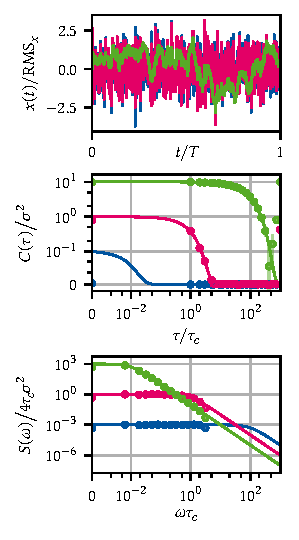
\includegraphics{img/pdf/spectrometer/lorentzian_psdcorr}
    \caption[\imgsource{img/py/spectrometer/lorentz.py}]{
        Ornstein-Uhlenbeck process.
        Simulated time traces (top), autocorrelation function (middle), \gls{psd} (bottom) of the Ornstein-Uhlenbeck process.
        Top: Simluated time traces using the algorithm presented in \cref{ch:ff:time_domain_methods}.
        The data are normalized to the computed \gls{rms} (equal to $\sigma$ in the continuous case).
        Middle: Theoretical autocorrelation function (\cref{eq:speck:ou:autocorrelation}, solid lines) and computed from the simulated data averaged over \num{e3} traces (circles, subset of points).
        Error bars indicate the standard error of the mean, axes are scaled with respect to the parameters of the magenta data, and data are plotted on an $\asinh$-scale.
        Bottom: Theoretical \gls{psd} (\cref{eq:speck:ou:psd}, solid lines) and periodograms computed from the simulated data using \code{scipy.signal.periodogram()}, \cf \cref{eq:speck:periodogram}, averaged over \num{e3} traces (circles, subset of points).
        Axes are again scaled with respect to the parameters of the magenta data and plotted on an $\asinh$-scale.
        Parameters are $\tau_c = \dt\times\{\num{e-2},\num{e0},\num{e2}\}$ and $\sigma^2=\sqrt{\tau_c}/4$ for blue, magenta, and green data, respectively.
    }
    \label{fig:speck:psdcorr}
\end{marginfigure}

To become familiar with the quantities $C(\tau)$ and $S(\omega)$, consider the Ornstein-Uhlenbeck process~\cite{Uhlenbeck1930}, the only stationary Gaussian Markovian stochastic process~\cite{VanKampen1976}.
The autocorrelation function of the Ornstein-Uhlenbeck process is given by
\begin{align}\label{eq:speck:ou:autocorrelation}
    C(\tau) = \sigma^2\e^{-\flatfrac{\tau}{\tau_c}},
\end{align}
with $\sigma$ the \gls{rms} and $\tau_c$ the correlation time of the process.
The \gls{psd} in turn is the Lorentzian function
\begin{align}\label{eq:speck:ou:psd}
    S(\omega) = \frac{2\sigma^2\tau_c}{1 + (\omega\tau_c)^2}.
\end{align}
For a given discretization time step \dt and hence bandwidth $\omega\in [0, \pi\fs]$, the Ornstein-Uhlenbeck process interpolates between perfectly uncorrelated, white noise ($\flatfrac{\dt}{\tau_c}\to\infty, S(\omega) = 2\tau_c\sigma^2$), correlated, Brownian noise ($\flatfrac{\dt}{\tau_c}\gg 1, S(\omega) = \flatfrac{2\sigma^2}{\tau_c\omega^2}$), and perfectly correlated, quasistatic noise ($\flatfrac{\dt}{\tau_c}\to 0, S(\omega) = \sigma^2\delta(\omega)$).
\Cref{fig:speck:psdcorr} depicts simulated data and its autocorrelation function and \gls{psd} for exemplary parameters: in the white noise limit ($\tau_c = \num{e-2}\dt$, blue), in the intermediate regime ($\tau_c = \dt$, magenta), and in the correlated regime ($\tau_c = \num{e+2}\dt$, green).
From the time series plot at the top it becomes clear that the \gls{rms} alone is insufficient to describe the properties of noisy signals as the curves differ significantly despite being normalized to their \gls{rms}.
The autocorrelation functions averaged over \num{e3} realizations of the noisy signals as well as their theoretical (continuous) value, \cref{eq:speck:ou:autocorrelation}, are plotted in the middle panel, normalized to $\tau_c=\dt$ and $\sigma^2=\flatfrac{\dt}{4}$.
For the white noise limit (blue), correlations are too short to be resolved with the given time discretization.
The correlations decay to $\e\inverse$ at $\flatfrac{\tau}{\tau_c}=\num{e-2},\num{e0},\num{e+2}$, respectively.
Finally, the bottom panel shows the \gls{psd}, \cref{eq:speck:ou:psd}, and its periodogram estimate, again averaged over \num{e3} realizations of the signal and normalized to $\tau_c=\dt$ and $\sigma^2=\flatfrac{\dt}{4}$.
The cross-over from white to Brownian \gls{psd} occurs at $\omega = \tau_c$.
While the simulated data for $\tau_c = \num{e-2}\dt$ appears perfectly white, that for $\tau_c = \num{e2}\dt$ appears perfectly \oneoverf-like because the spectrum is only white below the smallest resolvable frequency $\df = T\inverse$.

Having gotten an intuition for the quantities $C(\tau)$ and $S(\omega)$, let us move on to see how the latter may be obtained from time series data.
\Cref{eq:speck:psd:definition} represents the starting point for the experimental spectrum estimation procedure.
Instead of a continuous signal $x(t), t\in [0, T]$, consider its discretized version\sidenote{
    We only discuss the problem of equally spaced samples here.
    Variants for spectral estimation of time series with unequal spacing exist~\cite{Lomb1976,Scargle1982}.
}
\begin{align}\label{eq:speck:signal:discrete}
    x_n \qc n\in\lbrace 0, 1, \dotsc, N - 1\rbrace
\end{align}
defined at times $t_n = n\dt$ with $T = N\dt$ and where $\dt = \fs\inverse$ is the sampling interval (the inverse of the sampling frequency \fs).
Invoking the ergodic theorem,\sidenote{
    Note that the limit of perfectly correlated noise, $S(\omega)\propto\delta(\omega)$, technically does \emph{not} correspond to an ergodic process because $C(\tau)=\text{const.}\,\forall\tau\in(-\infty,\infty)$.
    In practice, this is always a mathematical idealization and the spectrum is actually better described by a nascent $\delta$-function with a small but finite width.
}
we can replace the long-term average in \cref{eq:speck:psd:definition} by the ensemble average over $M$ realizations of the noisy signal, $\left\lbrace x_n\gth{m}\right\rbrace_m$, and write
\begin{align}\label{eq:speck:psd:bartlett}
    S_n &= \frac{1}{M} \sum_{m=0}^{M-1} \abs{\hat{x}_n\gth{m}}^2 \\
        &= \frac{1}{M} \sum_{m=0}^{M-1} S_n\gth{m}
\end{align}
where $\hat{x}_n\gth{m}$ is the discrete Fourier transform of $x_n\gth{m}$, we defined the \emph{periodogram} of $x_n\gth{m}$ by
\begin{align}\label{eq:speck:periodogram}
    S_n\gth{m} = \abs{\hat{x}_n\gth{m}}^2,
\end{align}
and $S_n$ is an \emph{estimate} of the true \gls{psd} sampled at the discrete frequencies $\omega_n = \flatfrac{2\pi n}{T} \in 2\pi\times\lbrace\flatfrac{-\fs}{2}, \dotsc, \flatfrac{\fs}{2}\rbrace$.\sidenote{
    We blithely disregard integer algebra issues occuring here for conciseness and leave it as an exercise for the reader to figure out what the exact bounds of the set of $\omega_n$ are.
}
\Cref{eq:speck:psd:bartlett} is known as Bartlett's method~\cite{Bartlett1948} for spectrum estimation.\sidenote{
    \label{sidenote:continuum_limit}
    By taking the limit $M\to\infty$ one recovers the true \gls{psd}, \[\lim_{M\to\infty}S_n = S(\omega_n).\]
    The continuum limit is as always obtained by sending $\dt\to 0, N\to\infty, N\dt=\text{const}$.
}

To better understand the properties of this estimate, let us take a look at the parameters $\dt$, $N$, and $M$.
The sampling interval $\dt$ defines the largest resolvable frequency by the Nyquist sampling theorem,
\begin{align}\label{eq:speck:f_max}
    \fmax = \frac{\fs}{2} = \frac{1}{2\dt}.
\end{align}
In turn, the number of samples $N$ determines the frequency resolution $\df$, or smallest resolvable frequency,
\begin{align}\label{eq:speck:f_min}
    \fmin = \df = \frac{1}{T} = \frac{1}{N\dt} = \frac{\fs}{N}.
\end{align}
Lastly, $M$ determines the variance of the set of periodograms $\bigl\lbrace S_n\gth{m}\bigr\rbrace_{i=0}^{M-1}$ and hence the accuracy of the estimate $S_n$.

In practice, the ensemble realizations $i$ are of course obtained sequentially, implying that one acquires a time series of data $x_n, n\in\lbrace0, 1, \dotsc, NM - 1\rbrace$ and partitions these data into $M$ sequences of length $N$.
It becomes clear, then, that the Bartlett average (\cref{eq:speck:psd:bartlett}) trades spectral resolution (larger $N$) for estimation accuracy (larger $M$) given the finite acquisition time $T = NM\dt$.

An improvement in data efficiency can be achieved using Welch's method~\cite{Welch1967}.
To see how, we first need to discuss spectral windowing.

\section{Window functions}\label{sec:speck:theory:windows}
Partitioning a signal $x_n$ into $M$ sections $x_n\gth{m}$ of length $N$ is mathematically equivalent to multiplying the signal with the rectangular \emph{window function} given by\sidenote{
    This window is also known as the boxcar or Dirichlet window.
}
\begin{align}\label{eq:speck:window:boxcar}
    w_n\gth{m} =
    \begin{dcases}
        1 &\qif* (m - 1) N \leq n < m N\qand \\
        0 &\qelse*
    \end{dcases}
\end{align}
so that $x_n\gth{m} = x_n w_n\gth{m}$.
Now recall that multiplication and convolution are duals under the Fourier transform, implying that
\begin{align}\label{eq:speck:window:ft_pairs}
    \hat{x}_n\gth{m} = \hat{x}_n \ast \hat{w}_n\gth{m},
\end{align}
where the Fourier representation of the rectangular window\sidenote{
    $\sinc(x) = \flatfrac{\sin(x)}{x}$.
}
\begin{align}
    \hat{w}_n\gth{m} &= \hat{w}_n \e^{-\i(m - \flatfrac{1}{2})\omega_n T}, \label{eq:speck:window:boxcar:fourier}\\
             \hat{w}_n &= T\sinc\left(\frac{\omega_n T}{2}\right). \label{eq:speck:window:boxcar:fourier:unshifted}
\end{align}
\Cref{fig:speck:boxcar_fourier} shows the unshifted rectangular window $\hat{w}_n$ in Fourier space.
We can hence understand the Fourier spectrum of $x_n\gth{m}$ as sampling $\hat{x}_n$ with the probe $\hat{w}_n\gth{m}$.
However, whereas in the continuum limit (see \cref{sidenote:continuum_limit}) \cref{eq:speck:window:boxcar:fourier:unshifted} tends towards $\delta(\omega_n)$ and thus will produce a faithful reconstruction of the true spectrum, the finite sample rate $\fs$ of discrete signals and observation length $T$ induce finite frequency sampling and bandwidth of the probe as well as \emph{sidelobes}.\sidenote{
    For the optically inclined: this is akin to Fraunhofer diffraction at an aperture.
}
These effects incur what is known as \emph{spectral leakage} and \emph{scalloping loss}, respectively, and lead to artifacts and deviations of the spectrum estimator $S_n$ from the true spectrum $S(\omega_n)$~\cite{Harris1978,Koopmans1995}.

\begin{marginfigure}
    \centering
    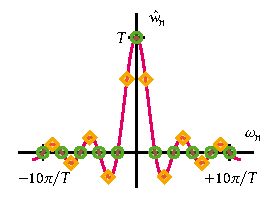
\includegraphics{img/pdf/spectrometer/rect}
    \caption[\imgsource{img/py/spectrometer/pyspeck.py}]{
        The Fourier representation of the rectangular window in continuous time (solid line) and for discrete frequencies $\omega_n = \flatfrac{2\pi n}{T}$ (circles).
        Introducing a phase shift, that is, shifting the window with respect to the signal in time, effectively shifts $\omega_n \to \omega_{n+\eta}$ as indicated for $\eta=\flatfrac{1}{2}$ (diamonds).
        This incurs scalloping loss.
    }
    \label{fig:speck:boxcar_fourier}
\end{marginfigure}

For this reason, a plethora of \emph{window functions} have been introduced to mitigate the effects of spectral leakage.
Key properties of a window are the spectral bandwidth (center lobe width) and sidelobe amplitude between which there typically is a tradeoff.\sidenote{
    Wikipedia gives a good overview of existing window functions~\cite{WindowFunctionWiki}.
}
A window frequently used in spectral analysis is the Hann window~\cite{Nuttall1981},
\begin{align}\label{eq:speck:window:hann}
    w_n\gth{m} =
    \begin{dcases}
        \sin^2\left(\frac{\pi n}{N}\right) &\qif* (m - 1)N\leq n < mN\qand \\
        0 &\text{else},
    \end{dcases}
\end{align}
with the Fourier representation of the unshifted window,
\begin{align}\label{eq:speck:window:hann:fourier_unshifted}
    \hat{w}_n &= \frac{T}{2}\sinc\left(\frac{\omega_n T}{2}\right)
                 %  \frac{1}{2(1 - \flatfrac{\omega_n T}{2\pi})(1 + \flatfrac{\omega_n T}{2\pi})},
                    \frac{1}{1 - \left(\flatfrac{\omega_n T}{2\pi}\right)^2}
\end{align}
shown in \cref{fig:speck:hann_fourier}.
The favorable properties of the Hann window are apparent when compared to the rectangular window in \cref{eq:speck:window:boxcar:fourier:unshifted} and \cref{fig:speck:boxcar_fourier}; the sidelobes are quadratically suppressed while the center lobe is broadened by a factor of two.

\begin{marginfigure}
    \centering
    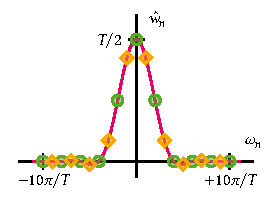
\includegraphics{img/pdf/spectrometer/hann}
    \caption[\imgsource{img/py/spectrometer/pyspeck.py}]{
        The Fourier representation of the Hann window in continuous time (solid line) and for discrete frequencies $\omega_n$ (circles).
        Diamonds indicate discrete sampling when the window completely out of phase with the signal (\cf \cref{fig:speck:boxcar_fourier}).
    }
    \label{fig:speck:hann_fourier}
\end{marginfigure}

Another favorable property of the Hann window is that $w_0\gth{0} = w_{N-1}\gth{0} = 0$.
This suppresses detrimental effects arising from a possible discontinuity ($x_0\gth{0}\neq x_{N-1}\gth{0}$) at the edge of a data segment related to the discrete Fourier transform, which assumes periodic data.\sidenote{
    Although this can usually also be achieved approximately by detrending the data before performing the Fourier transform, which is a good idea in any case.
}

\section{Welch's method}\label{sec:speck:theory:welch}
Contemplating \cref{eq:speck:window:hann}, one might come to the conclusion that using a window such as this is not very data efficient in the sense that a large fraction of samples located at the edge of the window is strongly suppressed and hence does not contribute significantly to the spectrum estimate.
To alleviate this lack of efficiency, one can introduce an overlap between adjacent data windows.
That is, instead of partitioning the data $x_n$ into $M$ non-overlapping sections of length $N$, one shifts the $m$th window forward by $-mK$ with $K>0$ the overlap.
Finally, the periodogram (\cref{eq:speck:periodogram}) is computed for each window and subsequently averaged to obtain the spectrum estimator (\cref{eq:speck:psd:bartlett}).

This method of spectrum estimation is known as Welch's method~\cite{Welch1967}.
One can show~\cite{Welch1967} that the correlation between the periodograms of adjacent, overlapping windows is sufficiently small to avoid a biased estimate.
The overlap naturally depends on the choice of window; a typical value for the Hann window $K = \flatfrac{N}{2}$ with which one would obtain $M = \flatfrac{2L}{N} - 1$ windows for data of length $L$.\sidenote{
    Again neglecting integer arithmetic issues.
}
\begin{figure}
    \centering
    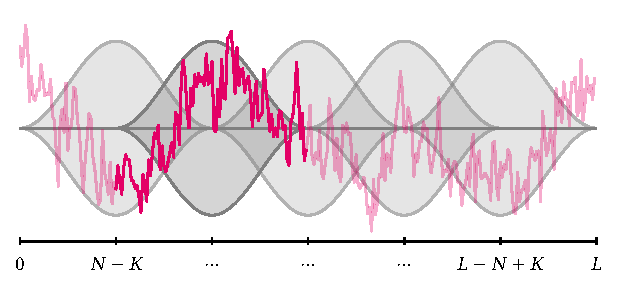
\includegraphics[width=\textwidth]{img/pdf/spectrometer/welch}
    \caption[\imgsource{img/py/spectrometer/pyspeck.py}]{
        Illustration of Welch's method for spectrum estimation.
        The data (magenta) of length $L$ is partitioned into $K = \flatfrac{2L}{N} - 1$ segments of length $N$.
        Each segment is multiplied with a window function (gray) which reduces spectral leakage and other artifacts.
        A finite overlap $K$ between adjacent windows (gray) ensures efficient sample use.
    }
    \label{fig:speck:welch}
\end{figure}

\Cref{fig:speck:welch} conceptually illustrates Welch's method for a trace of \oneoverf noise with $L = 300$ samples in total.
Choosing the Hann window and an overlap of \qty{50}{\percent} results in $M=5$ segments for a window length of $N=100$.
The data in the second window is highlighted.

\section{Parameters \& Properties of the \acrshort{psd}}\label{sec:speck:theory:welch:parameters}
\begin{margintable}[*-7]
    \centering
    \footnotesize
    \caption[Overview of spectrum estimation parameters]{
        Overview of spectrum estimation parameters.
        The parameters can be assigned into four groups
        \begin{enumerate*}[
            before=\unskip{: }, itemjoin={{, }}, itemjoin*={{, and }}
        ]
            \item \acrshort{daq} parameters configuring the \acrlong{daq} device
            \item Welch parameters specifying the periodogram averaging
            \item Spectrum properties induced by the above
            \item External parameters unrelated to the others
        \end{enumerate*}.
    }
    \label{tab:speck:theory:parameters}
    \renewcommand{\arraystretch}{1.1}
    \begin{tabularx}{\marginparwidth}{ c l }
        \multicolumn{2}{l}{\textsc{1. \acrshort{daq} parameters}} \\
        \toprule
        $L$ & Total number of samples \\
        \fs & Sample rate \\
        [0.5ex]
        \multicolumn{2}{l}{\textsc{2. Welch parameters}} \\
        \toprule
        $K$ & Number of overlap samples \\
        $N$ & Number of segment samples \\
        $M$ & Number of Welch segments \\
        [0.5ex]
        \multicolumn{2}{l}{\textsc{3. Spectrum parameters}} \\
        \toprule
        \fmin & Smallest resolvable frequency \\
        \fmax & Largest resolvable frequency \\
        [0.5ex]
        \multicolumn{2}{l}{\textsc{4. Miscellaneous parameters}} \\
        \toprule
        $O$ & Number of outer averages \\
    \end{tabularx}
\end{margintable}
We are now in a position to discuss how the various parameters of a time series relate to both the physical parameters of the resulting spectrum estimate and to each other.
To this end, we will go through the typical procedure of acquiring a spectrum estimate using Welch's method chronologically.

To acquire data using some form of (digital) \gls{daq}, one usually needs to specify two parameters first: the total number of samples to be acquired, $L$, and the sample rate \fs.
This results in a measurement of duration $T = L\dt$ where $\dt = \fs\inverse$ as previously mentioned.
The choice of \fs already induces an upper bound on the first parameter characterizing the \gls{psd} estimate: the largest resolvable frequency $\fmax\leq\flatfrac{\fs}{2}$ (\cf \cref{eq:speck:f_max}, but note that we allow \fmax to be smaller than half the sample rate in anticipation of hardware constraints).
Next, we choose a number of Welch averages, $M$, \ie, data partitions, and their overlap, $K$.
In doing so, one fixes the number of samples per partition $N$ and thereby induces the lower bound on the second parameter characterizing the \gls{psd} estimate: the frequency spacing $\df = \flatfrac{1}{N} \leq \fmin$ (\cf \cref{eq:speck:f_min}).\sidenote[][*-3]{
    Technically, the smallest resolvable frequency in a \gls{fft} is zero, of course. But as data is typically detrended (a constant or linear trend subtracted) before computation of the periodogram, the smallest \emph{meaningful} frequency is given by \fmin.
}
% TODO: be consistent in use of segment vs partition?
Finally, we can introduce a number of \emph{outer} averages $O$, that is, the number of data batches that are acquired.
While not directly related to Welch's method, choosing $O > 1$ can, for instance, help achieve a certain variance if the number of samples per batch, $L$, is limited by the \acrlong{daq} hardware, or simply allow for updating the spectrum estimate as data is being acquired.
\Cref{fig:speck:theory:parameters} shows the relationships of the various parameters among each other.
In \cref{subsec:speck:software:design:daq}, I lay out how these inter-dependencies are implemented in software.

\begin{figure}
    \centering
    \begin{tikzpicture}[
    >=stealth,
    auto,
    box/.style={
        draw,
        rectangle,
        rounded corners,
        thick,
        align=center,
        inner sep=2mm,
%        drop shadow,
    },
    float1/.style={box, fill=RWTHmagenta25, text=RWTHmagenta100},
    float2/.style={box, fill=RWTHmagenta10, text=RWTHmagenta75},
    int1/.style={box, fill=RWTHgreen25, text=RWTHgreen100},
    int2/.style={box, fill=RWTHgreen10, text=RWTHgreen75},
    int3/.style={box, fill=RWTHblack10, text=RWTHblack100},
]

    % Central node: nperseg
    \node[int1] (nperseg) {$N$};

    % Frequency branch: relative to nperseg, all nodes placed at the same x-coordinate.
    \node[float1, above left=1cm of nperseg, anchor=center] (fs) {\fs};
    \node[float1, below left=1cm of nperseg, anchor=center] (df) {\df};
    \node[float2, left=of fs] (fmax) {\fmax};
    \node[float2, left=of df] (fmin) {\fmin};

    % Segmentation branch: relative to nperseg
    \node[int2, right=of nperseg] (npts) {$L$};
    \node[int2, above right=of npts, anchor=center] (noverlap) {$K$};
    \node[int2, below right=of npts, anchor=center] (nseg) {$M$};

    % Stand-alone node for n_avg
    \node[int3, above=1cm of $(npts)!0.5!(nperseg)$] (navg) {$O$};

    % Draw frequency branch arrows
    \draw[->] (nperseg) -- (fs);
    \draw[->] (nperseg) -- (df);
    \draw[<->] (df) to[bend left=45] (fs);
    \draw[->] (fs) to[bend right=45] (fmax);
    \draw[->] (df) to[bend left=45] (fmin);
    \draw[<->] (fs) -- (nperseg);
    \draw[<->] (df) -- (nperseg);

    % Draw segmentation branch arrows (nperseg, noverlap, and n_seg together inform n_pts)
    \draw[<->] (nperseg) -- (npts);
    \draw[->] (noverlap) -- (npts);
    \draw[->] (nseg) -- (npts);

    % n_avg remains independent (no arrows drawn)

\end{tikzpicture}

    \caption[\imgsource{img/tikz/spectrometer/daq_settings.tex}]{
        Relationships of data acquisition parameters (\cf \cref{tab:speck:theory:parameters,tab:speck:software:parameters}, with arrows indicating dependencies.
        $N$, \fs, and \df are the central quantities defining the estimated spectrum's properties.
        From \fs and \df follow (bounds for) \fmax and \fmin.
        From $N$, together with $K$ and $M$, follows $L$, the total number of samples per data batch.
    }
    \label{fig:speck:theory:parameters}
\end{figure}

To conclude this chapter, let us discuss some of the properties of stochastic processes and their autocorrelation function and \gls{psd}.
Consider again the process $x(t)$.
We say $x(t)$ is \emph{Gaussian} if $x(t)\sim\mathcal{N}(\mu, \sigma^2)\,\forall t$, meaning that the value of $x(t)$ at a given point in time follows a normal distribution with some mean $\mu$ and variance $\sigma^2$ over multiple realizations of the process.
In this case, its statistical properties are fully described by the autocorrelation function $C(\tau)$ and \gls{psd} $S(\omega)$.
This is because only the first two cumulants of a Gaussian distribution are nonzero~\cite{Fox1978}.
For the purpose of noise estimation, the assumption of Gaussianity is a rather weak one as the noise typically arises from a large ensemble of individual fluctuators and is therefore well approximated by a Gaussian distribution by the central limit theorem~\cite{Krzywda2020}.\sidenote{
    As an example, consider electronic devices, where voltage noise is thought to arise from a large number of defects and other charge traps in oxides being populated and depopulated at certain rates $\gamma$. The ensemble average over these so-called \glspl{tlf} then yields the well-known \oneoverf-like noise spectra~\cite{Schriefl2006,Beaudoin2015} (at least for a large density~\cite{Mehmandoost2024}).
}
Even if $x(t)$ is not perfectly Gaussian, non-Gaussian contributions can be seen as higher-order contributions if viewed from the perspective of perturbation theory, and therefore the \gls{psd} still captures a significant part of the statistical properties.
For this reason, the \gls{psd} is the central quantity of interest in noise spectroscopy.
Let us just note at this point that techniques to estimate higher-order spectra (or \emph{polyspectra}) exist~\cite{Chandran1994,Norris2016,Szankowski2017}.

For real signals $x(t)\in\mathbb{R}$, the autocorrelation function $C(\tau)$ is an even function, while for $x(t)\in\mathbb{C}$ its real part is even and its complex part odd.
From this it immediately follows that for real $x(t)$ $S(\omega)$ is also an even function and one therefore distinguishes the \emph{two-sided} \gls{psd} $S^{(2)}(\omega)$ defined over $\mathbb{R}$ from the \emph{one-sided} \gls{psd} $S^{(1)}(\omega) = 2 S^{(2)}(\omega)$ defined only over $\mathbb{R}^+$.
Complex $x(t)$ such as those generated by \glspl{lia} after demodulation in turn have asymmetric, two-sided \glspl{psd}.
In this chapter so far, we have implicitly employed the two-sided definition, but in the software package presented in \cref{ch:speck:software}, two-sided spectra are used only for complex data since they contain redundant information for real data.

% mainfile: ../../main.tex
\chapter{The \pyspeck software package}\label{ch:speck:software}
\mylettrine{I}{n} this chapter, I introduce the \pyspeck \python package\sidenote{
    The package repository is hosted on \href{https://git.rwth-aachen.de/qutech/python-spectrometer/}{GitLab}.
    Its documentation is automatically generated and hosted on \href{https://qutech.pages.rwth-aachen.de/python-spectrometer/}{GitLab Pages}.
    Releases are automatically published to \href{https://pypi.org/project/python-spectrometer/}{PyPI} and allow the package to be installed using \code{pip install python-spectrometer}.
}
and lay out its design and functionality.
This software package was developed to make it easier for experimentalists to transfer the mathematical machinery introduced in \cref{ch:speck:theory} to the lab.
While in principle the entire process of spectrum estimation from a given array of time series data is already covered by the \code{welch()} routine in \scipy~\sidecite{WelchScipy}, obtaining the data array is not standardized.
Different \gls{daq} instruments have different capabilities, both on the hardware and the software level, and different driver interfaces to communicate with them.
This implies custom \acrlong{daq} code is required for every instrument, introducing a significant entry barrier to spectral analysis.
The \pyspeck package implements a simple interface to different hardware instruments that allows for changing the hardware backend without having to adapt the user-facing code and also incorporates different hardware constraints.

What is more, noise spectroscopy tends to be a visual endeavor in practice; it is hard to compare different noise spectra based on quantitative reasoning alone.
Data visualization is hence an integral part of noise spectroscopy, but plotting is not just plotting.
Do we want the data to be shown on a log-log scale?\sidenote{
    The short answer is yes, but it comes with visual side-effects that demand other ways of plotting data at times.
    The long answer is therefore yes, \emph{and} \dots
}
Do we want to show the relative magnitude of different data sets?
Do we want to inspect the time traces as well?
The \pyspeck package addresses these questions by allowing users to interactively change features of the main plot window to adapt it to the form best suited to the situation at hand.

Moreover, when concerned with noise spectrum estimation, we are typically more interested in specifying parameters of the resulting \gls{psd} rather than parameters of the underlying time series data.
The \pyspeck package approaches \acrlong{daq} from the inverse direction: rather than inferring the spectrum properties from the time series data, users specify the properties they would like the resulting spectrum to have and the package chooses the correct parameters for \acrlong{daq} accordingly.

\section{Package design and implementation}\label{sec:speck:software:design}
\begin{marginfigure}[-3.75cm]
    \forestset{
    dir tree/.style={
        for tree={
            parent anchor=south west,
            child anchor=west,
            anchor=mid west,
            inner ysep=0pt,
            grow'=0,
            align=left,
            s sep=1ex,
            edge path={
                \noexpand\path [draw, \forestoption{edge}] (!u.parent anchor) ++(0.75em,0) |- (.child anchor)\forestoption{edge label};
            },
            font=\footnotesize\ttfamily,
            if n children=0{}{
                delay={
                    prepend={[,phantom, calign with current]}
                }
            },
            fit=band,
            before computing xy={
                l=1.5em
            }
        },
    }
}
\begin{forest}
    dir tree
    [
        [{\faIcon[regular]{folder} \pyspeckpath{doc}{doc}}]
        [{\faIcon[regular]{folder-open} \pyspeckpath{src}{src}}
            [{\faIcon[regular]{folder-open} \pyspeckpath{src/python_spectrometer}{python\_spectrometer}}
                [{\faIcon[regular]{folder-open} \pyspeckpath{src/python_spectrometer/daq}{daq}}
                    [{\faIcon[regular]{file-code} \pyspeckpath{src/python_spectrometer/daq/__init__.py}{\_\_init\_\_.py}}]
                    [{\faIcon[regular]{file-code} \pyspeckpath{src/python_spectrometer/daq/base.py}{base.py}}]
                    [{\faIcon[regular]{file-code} \pyspeckpath{src/python_spectrometer/daq/qcodes.py}{qcodes.py}}]
                    [{\faIcon[regular]{file-code} \pyspeckpath{src/python_spectrometer/daq/settings.py}{settings.py}}]
                    [{\faIcon[regular]{file-code} \ldots}]
                ]
                [{\faIcon[regular]{file-code} \pyspeckpath{src/python_spectrometer/__init__.py}{\_\_init\_\_.py}}]
                [{\faIcon[regular]{file-code} \pyspeckpath{src/python_spectrometer/_audio_manager.py}{\_audio\_manager.py}}]
                [{\faIcon[regular]{file-code} \pyspeckpath{src/python_spectrometer/_plot_manager.py}{\_plot\_manager.py}}]
                [{\faIcon[regular]{file-code} \pyspeckpath{src/python_spectrometer/core.py}{core.py}}]
            ]
        ]
        [{\faIcon[regular]{folder} \pyspeckpath{tests}{tests}}]
        [{\faIcon[regular]{file-code} \pyspeckpath{pyproject.toml}{pyproject.toml}}]
        [{\faIcon[regular]{file-code} \ldots}]
    ]
\end{forest}

    \caption[Source tree structure of the \pyspeck package.]{
        Source tree structure of the \pyspeck package.
        Driver wrappers are placed in the \code{daq} subpackage.
        \code{core.py} exports the \code{Spectrometer} class.
    }
    \label{fig:speck:software:tree}
\end{marginfigure}
The \pyspeck package provides a central class, \code{Spectrometer}, that users interact with to perform data acquisition, spectrum estimation, and plotting.
It is instantiated with an instance of a child class of the \code{DAQ} base class that implements an interface to various \gls{daq} hardware devices.\sidenote[][4.6cm]{
    Actually \emph{drivers} to be more precise.
}
New spectra are obtained by calling the \code{Spectrometer.take()} method with all acquisition and metadata settings.
In the following, I will go over the the design of these aspects of the package in more detail.

\subsection{Data acquisition}\label{subsec:speck:software:design:daq}
\Cref{fig:speck:software:tree} shows the directory structure of the source code.
The \code{daq} subpackage contains on the one hand the declaration of the \code{DAQ} abstract base class (\code{base.py}) and its child class implementations (\code{qcodes.py}, \etc), and on the other the \code{settings.py} module, which defines the \code{DAQSettings} class.
This class is used in the background to validate data acquisition settings both for consistency (see \cref{subsec:speck:theory:welch:parameters}) and hardware constraints.

\begin{margintable}
    \footnotesize
    \centering
    \setmintedinline[Python]{fontsize=\footnotesize}
    \caption[Overview of spectrum estimation parameters]{
        Variable names used in \cref{ch:speck:theory} and their corresponding parameter names as used in \pyspeck and \code{scipy.signal.welch()}~\cite{WelchScipy}.
    }
    \label{tab:speck:software:parameters}
    \begin{tabular}{ c C }
        \toprule
        Variable & Parameter \\
        \midrule
        $L$ & n_pts \\
        $N$ & nperseg \\
        $K$ & noverlap \\
        $M$ & n_seg \\
        $O$ & n_avg \\
        \fs & fs \\
        \fmax & f_max \\
        \fmin & f_min \\
        \bottomrule
    \end{tabular}
\end{margintable}

To better understand the necessity of this functionality, consider the typical scenario of a physicist\sidenote{
    Let's call her Alice.
}
in the lab.
Alice has wired up her experiment, performed a first measurement, and to her dismay discovered that the data is too noisy to see the sought-after effect.
She sets up the \pyspeck code to investigate the noise spectrum of her measurement setup.
From her noisy data she could already estimate the frequency of the most harrowing noise, so she knows the frequency band $[\fmin, \fmax]$ she is most interested in.
But because she is lazy,\sidenote{
    Physicists generally are.
}
she does not want to do the mental gymnastics to convert \fmin to the parameter that her \gls{daq} device understands, $L$ (see \cref{tab:speck:software:parameters}), especially considering that $L$ depends on the number of Welch averages and the overlap.
Furthermore, while she could just about do the conversion from \fmax to the other relevant \gls{daq} parameter, \fs, in her head, her device imposes hardware constraints on the allowed sample rates she can select!
The \code{DAQSettings} class addresses these issues.
It is instantiated with any subset of the parameters listed in \cref{tab:speck:software:parameters}\sidenote{
    \code{DAQSettings} inherits from the builtin \code{dict} and as such can contain arbitrary other keys besides those listed in \cref{tab:speck:software:parameters}.
    However, automatic validation of parameter consistency is only performed for these special keys.
}
and attempts to resolve the parameter interdependencies lined out in \cref{subsec:speck:theory:welch:parameters} upon calling \code{DAQSettings.to_consistent_dict()}.\sidenote{
    Since the graph spanned by the parameters is not acyclic, this only works \emph{most} of the time.
}
This either infers those parameters that were not given from those that were or, if not possible, uses a default value.
Child classes of the \code{DAQ} class can subclass \code{DAQSettings} to implement hardware constraints such as a finite set of allowed sampling rates or a maximum number of samples per data buffer.

For instance, Alice might want to measure the noise spectrum in the frequency band $[\qty{1.5}{\hertz}, \qty{72}{\kilo\hertz}]$.
Although she would not have to do this explicitly,\sidenote{
    Settings are automatically parsed when passed to the \code{take()} method of the \code{Spectrometer} class.
}
she could inspect the parameters after resolution using the code shown in \cref{lst:speck:daq:settings}.

\begin{listing}[htpb]
    \begin{py}
        >>> from python_spectrometer.daq import DAQSettings
        >>> settings = DAQSettings(f_min=1.5, f_max=7.2e4)
        >>> settings.to_consistent_dict()
        {'f_min': 1.5,
         'f_max': 72000.0,
         'fs': 144000.0,
         'df': 1.5,
         'nperseg': 96000,
         'noverlap': 48000,
         'n_seg': 5,
         'n_pts': 288000,
         'n_avg': 1}
    \end{py}
    \caption{
        \code{DAQSettings} example showcasing automatic parameter resolution.
        \code{n_avg} determines the number of outer averages, \ie, the number of data buffers acquired and processed individually.
    }
    \label{lst:speck:daq:settings}
\end{listing}

\begin{marginlisting}[-2.5cm]
    \begin{py}[fontsize=\footnotesize]
    {'f_min': 14.30511474609375,
     'f_max': 72000.0,
     'fs': 234375.0,
     'df': 14.30511474609375,
     'nperseg': 16384,
     'noverlap': 0,
     'n_seg': 1,
     'n_pts': 16384,
     'n_avg': 1}
    \end{py}
    \caption[Resolved \code{DAQSettings} for MFLI Scope]{
        Resolved settings for the same input parameters as in \cref{lst:speck:daq:settings} but for the \code{ZurichInstrumentsMFLIScope} backend with hardware constraints on \code{n_pts} and \code{fs}.
    }
    \label{lst:speck:daq:settings:mfli_scope}
\end{marginlisting}

If the instrument she'd chosen for data acquisition had been a Zurich Instruments MFLI's Scope module,\sidenote[][2.7cm]{
    \url{https://docs.zhinst.com/labone_api_user_manual/modules/scope/index.html}
}
the same requested settings would have resolved to those shown in \cref{lst:speck:daq:settings:mfli_scope}.\sidenote[][3.5cm]{
    And issued a warning to inform the user their requested settings could not be matched.
}
This is because the Scope module constrains $L\in[2^{12},2^{14}]$ and $\fs\in\qty{60}{\mega\hertz}\times 2^{[-16, 0]} \approx \allowbreak \lbrace \qty{915.5}{\hertz}, \allowbreak \dotsc, \allowbreak \qty{30}{\mega\hertz}, \qty{60}{\mega\hertz}\rbrace$.

As already mentioned, the \code{DAQ} base class implements a common interface for different hardware backends, allowing the \code{Spectrometer} class to be hardware agnostic.
That is, changing the instrument that is used to acquire the data does not necessitate adapting the code used to interact with the \code{Spectrometer}.
To enable this, different instruments require small wrapper drivers that map the functionality of their actual driver onto the interface dictated by the \code{DAQ} class.
This is achieved by subclassing \code{DAQ} and implementing the \code{DAQ.setup()} and \code{DAQ.acquire()} methods.
Their functionality is best illustrated by the internal workflow as representatively shown in \cref{lst:speck:daq:workflow}.

\begin{listing}[htpb]
    \begin{py}
        daq = MyDAQ(driver_handle)

        parsed_settings = daq.setup(**user_settings)
        acquisition_generator = daq.acquire(**parsed_settings)

        for data_buffer in acquisition_generator:
            estimate_psd(data_buffer)
    \end{py}
    \caption[\gls{daq} workflow pseudocode]{
        \gls{daq} workflow pseudocode.
        A \code{MyDAQ} object (representing the instrument \code{My}) is instantiated with a driver object (for instance a \href{https://github.com/microsoft/qcodes}{QCoDeS} \code{Instrument}).
        The instrument is configured with the given \code{user_settings}.
        Calling the generator function \code{daq.acquire()} with the actual device settings returns a generator, iterating over which yields one data buffer per iteration.
        The data buffers can then be passed to further processing functions (the \gls{psd} estimator in our example).
    }
    \label{lst:speck:daq:workflow}
\end{listing}

When acquiring a new spectrum, all settings supplied by the user are first fed into the \code{setup()} method where instrument configuration takes place.
The method returns the actual device settings,\sidenote{
    Which might differ from the requested settings as outlined above.
}
which are then forwarded to the \code{acquire()} generator function.
Here, the instrument is armed (if necessary), and subsequently data is fetched from the device and yielded to the caller \code{n_avg} times, where \code{n_avg} is the number of outer averages.\sidenote{
    \Ie, the number of time series data batches acquired, as opposed to the number of Welch averages \code{n_seg} within one batch.
}
An exemplary implementation of a \code{DAQ} subclass for a fictitious instrument is shown in \cref{lst:speck:daq:pseudocode}.
In addition to the methods to configure the instrument and perform data acquisition, it is possible to override the \code{DAQSettings} property to implement instrument-specific hardware constraints such as, in this example, the number of samples per buffer being constrained to the discrete interval $[1, 2048]$.
Leveraging the \code{qutil.domains} module, more complex constraints such as sample rates restricted to an internal clock rate divided by a power of two\sidenote{
    See for example the implementation of the \href{https://git.rwth-aachen.de/qutech/python-spectrometer/-/blob/main/src/python_spectrometer/daq/atsaverage.py}{AlazarTech ATS9440} digitizer card.
}
can be specified.

\begin{listing}
    \begin{py}
        # daq/mydaq.py
        import dataclasses
        from qutil.domains import DiscreteInterval
        from .base import DAQ
        from .settings import DAQSettings

        @dataclasses.dataclass
        class MyDAQ(DAQ):
            handle: mydriver.DeviceHandle

            @property
            def DAQSettings(self) -> type[DAQSettings]:
                class MyDAQSettings(DAQSettings):
                    ALLOWED_NPERSEG = DiscreteInterval(1, 2048)
                return MyDAQSettings

            def setup(self, **settings) -> dict:
                settings = self.DAQSettings(settings)
                parsed_settings = settings.to_consistent_dict()
                self.handle.configure(parsed_settings)
                return parsed_settings

            def acquire(self, n_avg: int, *, **settings) -> Generator:
                self.handle.arm(n_avg)
                for _ in range(n_avg):
                    self.handle.wait_for_trigger()
                    yield self.handle.fetch()
                return self.handle.metadata
    \end{py}
    \caption[\code{DAQ} pseudocode]{
        Exemplary code for a \code{DAQ} implementation of some instrument with given driver class \code{DeviceHandle} in the package \code{mydriver}.
        The \code{MyDAQ} class is instantiated with a \code{DeviceHandle} instance.
        Optionally, the \code{DAQSettings} property can be overridden to implement hardware constraints or default values for data acquisition parameters.
        For this, the \code{qutil.domains} module provides several classes that represent bounded domains and sets.
        The \code{setup()} method parses the given acquisition settings and configures the instrument through the external driver interface \code{handle.configure()}.
        The \code{acquire()} method arms the instrument (if necessary) and loops over the number of outer averages, \code{n_avg}.
        In the body of the loop, it can wait for external triggers (or send software triggers) before yielding a batch of data fetched from the external driver interface.
        Once acquisition is done, the method can return arbitrary metadata to the \code{Spectrometer} object to attach to the stored data.
    }
    \label{lst:speck:daq:pseudocode}
\end{listing}

\subsection{Data processing}\label{subsec:speck:software:design:processing}
Once time series data has been acquired using a given \code{DAQ} backend, it could in principle immediately be used to estimate the \gls{psd} following \cref{eq:speck:psd:bartlett}.
However, it is often desirable to transform, or process, the data in some fashion.
This can include simple transformations such as accounting for the gain of a \gls{tia} and convert the voltage back to a current,\sidenote{
    Although it is of course less than trivial to discriminate between current and voltage noise in a \gls{tia}.
}
or more complex ones such as applying calibrations.
In particular, since the process of computing the \gls{psd} already involves Fourier transformation, the processing can also be performed in frequency space.

In \pyspeck, this can be done using a \code{procfn} (in the time domain) or \code{fourier_procfn} (in the Fourier domain).
The former is specified as an argument directly to the \code{Spectrometer} constructor.
It is a callable with signature \code{(x, **kwargs) -> xp}, that is, takes the time series data as its first (positional) argument and arbitrary settings that are passed through from the \code{take()} method as keyword arguments, and returns the processed data.
\Cref{lst:speck:procfn} shows a simple function that accounts for the gain of an amplifier.
The latter is specified in the \code{psd_estimator} argument of the \code{Spectrometer} constructor.
This argument allows the user to specify a custom estimator for the \gls{psd}, in which case a callable is expected.
Otherwise, it should be a mapping containing parameters for the default \gls{psd} estimator, \code{scipy.signal.welch()}~\sidecite{WelchScipy}.
Here, the keyword \code{fourier_procfn} should be a callable with signature \code{(xf, f, **kwargs) -> (xfp, fp)}.\sidenote{
    \Ie, the \code{psd_estimator} argument would be \code{{"fourier_procfn": fn}}.
}
That is, it should take the frequency-space data, the corresponding frequencies, and arbitrary keyword arguments and return a tuple of the processed data and the corresponding frequencies.

\begin{marginlisting}
    \begin{py}[fontsize=\footnotesize]
        def comp_gain(x, gain=1.0, **_):
            return x / gain
    \end{py}
    \caption[Simple \code{procfn} example]{
        A simple \code{procfn}, which converts amplified data back to the level before amplification.
        Note the token \code{**_} variable keyword argument that ensures no errors arise from other parameters being passed to the function.
        More complex processing chains can concisely be defined with \code{qutil.functools.FunctionChain} that pipes the output of one function into the input of the next.
    }
    \label{lst:speck:procfn}
\end{marginlisting}

The latter are required in case the function modifies the frequencies.\sidenote{
    One example is the \code{octave_band_rms()} function from the \code{qutil.signal_processing} subpackage~\cite{OctaveBandRmsQutil} that decimates frequencies to fractions of octave bands. See \cref{part:setup} for a use-case. TODO: ref
}
A simple example for a processing function in Fourier space is shown in \cref{lst:speck:fourier_procfn}, which computes the \mbox{(anti-)}derivative of the data using the fact that
\begin{marginlisting}
    \begin{py}[fontsize=\footnotesize]
        def derivative(xf, f, n=0, **_):
            return xf / (2j * pi * f)**n
    \end{py}
    \caption[Simple \code{fourier_procfn} example]{A simple \code{fourier_procfn}, which calculates the \mbox{(anti-)}derivative.}
    \label{lst:speck:fourier_procfn}
\end{marginlisting}
\begin{align}\label{eq:speck:fourier_derivative}
    \pdv[n]{t} \xrightarrow{\mathrm{F.T.}} \left(\i\omega\right)^n
\end{align}
under the Fourier transform.
In \cref{part:setup}\todo{ref}, I discuss more complex use-cases of the processing functionality included in \pyspeck in the context of vibration spectroscopy.

\section{Feature overview}\label{sec:speck:software:features}
Now that we have a basic understanding of the design choices underlying \pyspeck, let us discuss the typical workflow of using the package.
Two modes of operation are to be distinguished: first, \enquote{serial} mode, in which users record new spectra manually, and second, \enquote{live} mode, in which new data is continuously being acquired.
The former is well suited to a structured approach to noise spectroscopy, where data is retained persistently and discrete changes are made to the system between data acquisitions.
The latter is aimed at a more fluent workflow in which data is not retained and data acquisition runs in the background.\todo{blabla}

\subsection{Serial spectrum acquisition}\label{subsec:speck:software:features:serial}
The default mode for spectrum acquisition using \pyspeck revolves around the \code{take()} method.
Key to this workflow is the idea that each acquired spectrum be assigned a comment that allows to easily identify it in the main plot.
For instance, this comment could contain information about the particular settings that were active when the spectrum was recorded, or where a particular cable was placed.

Consider as an example the procedure of \enquote{noise hunting}, \ie, debugging a noisy experimental setup.
The experimentalist,\sidenote{
    Let's call him Bob.
}
having discovered that his data is noisier than expected, sets up the \code{Spectrometer} class with an instance of the \code{DAQ} subclass for the \gls{daq} instrument connected to his sample, a Zurich Instruments MFLI.\sidenote{
    For the MFLI, \code{DAQ} subclasses for both the \href{https://docs.zhinst.com/labone_api_user_manual/modules/scope/index.html}{Scope} and the \href{https://docs.zhinst.com/labone_api_user_manual/modules/daq/index.html}{DAQ} module are implemented.
    The former gives access to the signal before and the latter to the signal after demodulation.
}
Choosing the frequency bounds, say $\fmin = \qty{10}{\hertz}$ and $\fmax = \qty{100}{\kilo\hertz}$, and using the sensible defaults for the remaining spectrum parameters, Bob first grounds the input of his \gls{daq} to record a \emph{baseline} spectrum.
Thus far, his code would hence look something like that shown in \cref{lst:speck:workflow:serial}, which produces the plot shown in \cref{fig:speck:software:workflow:baseline}.

\begin{listing}[htpb]
    \begin{py}
        from python_spectrometer import Spectrometer, daq
        from qutil.functools import scaled

        mfli_daq = daq.ZurichInstrumentsMFLIDAQ(session, device)
        spect = Spectrometer(mfli_daq, procfn=scaled(1e6),
                             processed_unit='μV')

        spect.take('baseline', f_min=1e1, f_max=1e5, daq='grounded')
    \end{py}
    \caption[\pyspeck serial workflow]{
        Setup and serial workflow using the \pyspeck package.
        \code{session} and \code{device} are \gls{api} objects of the \code{zhinst.toolkit} driver package.
        It is therefore possible to simply use the driver objects that are already in use in the measurement setup.
        The \code{procfn} and \code{processed_unit} arguments help converting raw data into a more human-friendly unit.
    }
    \label{lst:speck:workflow:serial}
\end{listing}
\begin{figure}
    \centering
    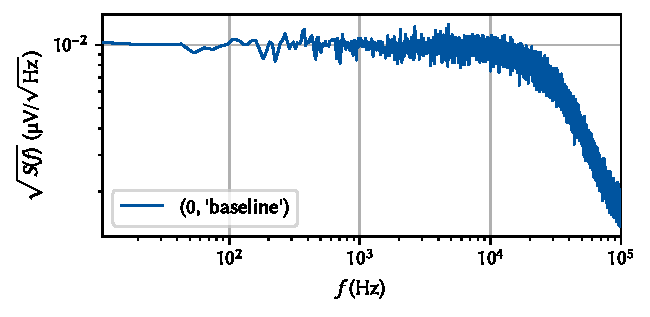
\includegraphics{pdf/spectrometer/workflow_baseline}
    \caption{
        The \pyspeck plot after acquiring the (here: synthetic) baseline spectrum.
        By default, the \gls{asd} = √\gls{psd} is displayed in the main plot.
        Each spectrum is assigned a unique identifier key consisting of an incrementing integer and the user comment, and can be refered to by either (or both) when interacting with the object.
    }
    \label{fig:speck:software:workflow:baseline}
\end{figure}

After acquiring the baseline, he next ungrounds the \gls{daq} to obtain a representative spectrum of the noise in an actual measurement.
He then proceeds by tweaking things on his setup, testing out different parameters, \etc
Every time he changes something, he acquires another spectrum using \code{take()}, labeling each with a meaningful comment for identification.
\begin{listing}[H]
    \begin{py}
        settings = {'f_min': 1e1, 'f_max': 1e5, 'daq': 'connected'}
        spect.take('connected', **settings)
        spect.take('lifted cable', cable='lifted', **settings)
        spect.take('jumped', **settings)
    \end{py}
    \caption[]{
        Code to acquire additional spectra.
        Arbitrary key-value pairs can be passed to the \code{take()} method, which are stored as metadata if they do not apply to any functions downstream in the data processing chain.
    }
    \label{lst:speck:workflow:spectra}
\end{listing}
\begin{figure}
    \centering
    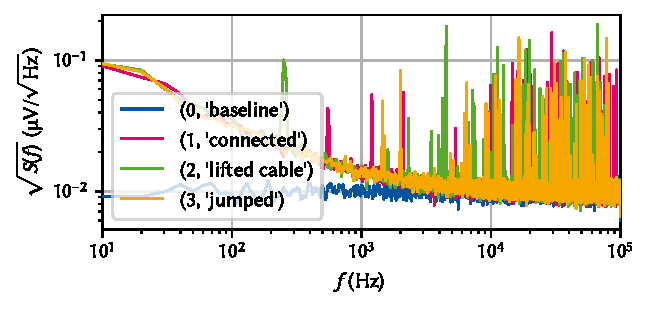
\includegraphics{pdf/spectrometer/workflow_spectra}
    \caption{
        The \pyspeck plot after acquiring additional (synthetic) spectra.
        Each spectrum is uniquely identified by a two-tuple of \code{(index, comment)}.
    }
    \label{fig:speck:software:workflow:spectra}
\end{figure}
The code shown in \cref{lst:speck:workflow:spectra} would then leave him with the spectrometer plot as shown in \cref{fig:speck:software:workflow:spectra}.
While working, Bob realizes he'd like see the signal in the time-domain as well.
He easily achieves this by setting \code{spect.plot_timetrace = True}, which adds an oscilloscope subplot to spectrometer figure as shown in \cref{fig:speck:software:workflow:timetrace}.

\begin{figure}
    \centering
    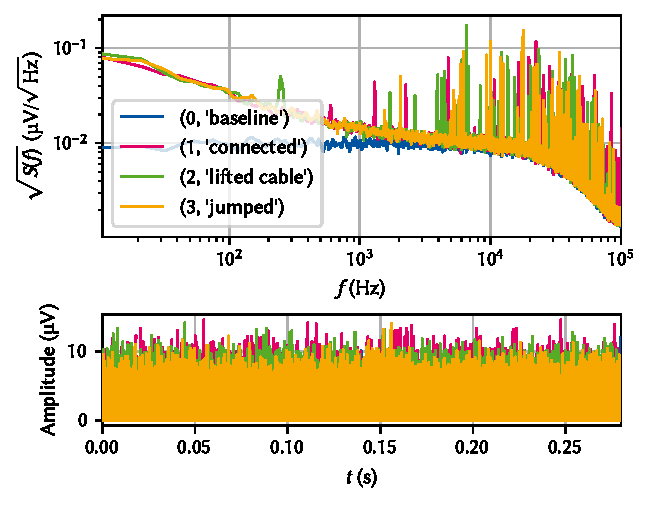
\includegraphics{pdf/spectrometer/workflow_timetrace}
    \caption{
        The \pyspeck plot shown in \cref{fig:speck:software:workflow:spectra} when setting \code{spect.plot_timetrace = True}.
        This adds a subplot that shows the time series data from which the \gls{psd} was computed akin to what an oscilloscope would show.
        Note that this is the entire time series, \ie, the data of length $L$, which is (by default, using Welch's method) segmented for spectrum estimation.
    }
    \label{fig:speck:software:workflow:timetrace}
\end{figure}

Bob now observes that the noise spectra he has recorded display many sharp peaks in particular at high frequencies while the \oneoverf noise floor seems pretty consistent across different measurements.
This makes it harder for him to evaluate whether any of his changes are actually an improvement or not.
The \pyspeck package allows addressing this by plotting the integrated spectra in another subplot.
Bob's spectrometer figure after setting \code{spect.plot_cumulative = True} is shown in \cref{fig:speck:software:workflow:cumulative}.
In the case that \code{spect.plot_amplitude == True}, this new subplot shows the \gls{rms} in the band $[\fmin, f]$,
\begin{align}\label{eq:speck:software:cumulative}
    \rms_S(f)\equiv\rms_S(\fmin, f),
\end{align}
and the band power (\cref{eq:speck:psd:bandpower}) otherwise.

\begin{figure}
    \centering
    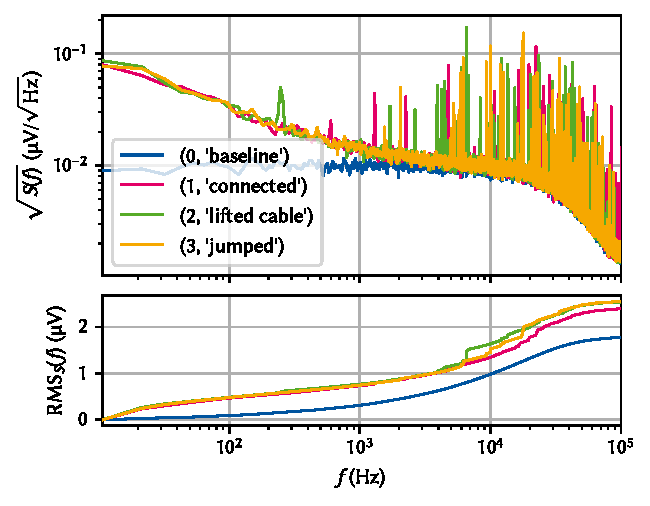
\includegraphics{pdf/spectrometer/workflow_cumulative}
    \caption{
        The \pyspeck plot shown in \cref{fig:speck:software:workflow:spectra} when setting \code{spect.plot_cumulative = True}.
        This adds a subplot that shows the \gls{rms} (see \cref{eq:speck:psd:bandpower}) which can be helpful in evaluating the contribution of individual peaks in the spectrum to the total noise power.
        Both the oscilloscope subplot (\cref{fig:speck:software:workflow:timetrace}) and the \gls{rms} subplot can also be shown at the same time.
    }
    \label{fig:speck:software:workflow:cumulative}
\end{figure}

The cumulative \gls{rms} plot already helps, but Bob would like a more quantitative comparison of relative spectral powers.
Therefore, he rescales the spectra in terms of their relative powers expressed in \unit{\decibel}\sidenote{
    Recall that the decibel is defined by the ratio $L_P$ of two powers $P_1, P_2$ as~\cite{Pozar2012}
    \begin{align*}
        L_P = 10\log_{10}\left(\frac{P_1}{P_2}\right)\,\unit{\decibel}.
    \end{align*}
}
by applying the following settings, which produces the plot shown in \cref{fig:speck:software:workflow:db}:
\begin{py}
    spect.plot_dB_scale = True
    spect.plot_amplitude = False
    spect.plot_density = False
\end{py}
\begin{figure}
    \centering
    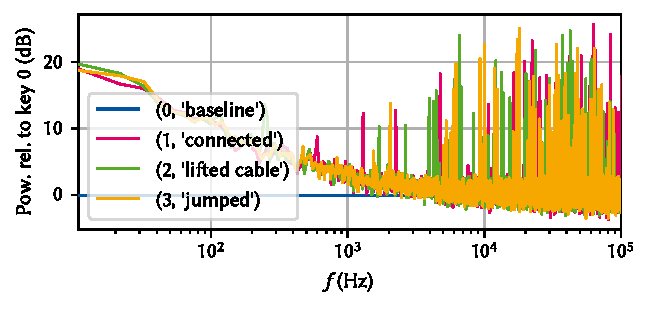
\includegraphics{pdf/spectrometer/workflow_db}
    \caption[The \pyspeck plot in relative mode.]{
        The \pyspeck plot in relative mode.
        Starting from the state in \cref{fig:speck:software:workflow:spectra}, we set \code{spect.plot_dB_scale = True} as well as \code{spect.plot_amplitude = False} and \code{spect.plot_density = False} to compare the relative noise powers with respect to the baseline.
    }
    \label{fig:speck:software:workflow:db}
\end{figure}
The attribute \code{plot_density} controls whether the \emph{\acrlong{psd}} or the \emph{power spectrum} is plotted.\sidenote{
    \label{sidenote:speck:software_vocabulary}
    At this point, we \emph{do} need to distinguish between the \gls{psd} and the power spectrum counter to \cref{sidenote:speck:theory_vocabulary} in \cref{ch:speck:theory}.
    The \gls{psd} and power spectrum are related by the \gls{enbw},
    \begin{align*}
        \text{Spectral density} \xrightarrow{\times\enbw} \text{Spectrum},
    \end{align*}
    which is itself a function of the sampling rate and the properties of the spectral window~\cite{Harris1978},
    \begin{align}\label{eq:speck:software:enbw}
        \enbw = \fs\frac{\sum_n\hat{w}_n^2}{\left[\sum_n\hat{w}_n\right]^2}.
    \end{align}
}
Scaling the data to the power spectrum instead of the density, Bob can get an estimate of the \gls{rms} at a single frequency by reading off the peak height.
Additionally displaying the data in \unit{\decibel} then gives insight into relative noise powers of different spectra.

Bob carries on with his enterprise and continues to acquire spectra until, finally, he finds the source of his noise!
Alas, his spectrometer plot is now overflowing with plotted data when really he just wants to compare the baseline, the original, noisy state, and the final, clean spectrum.
He simply calls
\begin{py}
    spect.hide(*range(2, 10))
\end{py}
to hide the eight spectra of unsuccessful debugging, leaving him with a plot as shown in \cref{fig:speck:software:workflow:success}.

\begin{figure}
    \centering
    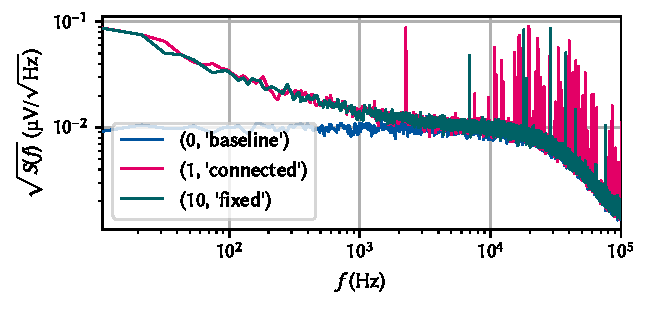
\includegraphics{pdf/spectrometer/workflow_success}
    \caption{
        The \pyspeck plot after multiple additional spectra were acquired and hidden.
        Hiding spectra that one is not interested in anymore is achieved through \code{spect.hide(*range(2, 10))}.
        This is reversed by \code{spect.show(*range(2, 10))}.
        Data can also be dropped (\code{spect.drop(key)}) or deleted (\code{spect.delete(key)}) from the internal cache and disk, respectively.
    }
    \label{fig:speck:software:workflow:success}
\end{figure}

Finally, happy with the results, Bob serializes the state of the spectrometer to disk, allowing him to pick up where he left off at a later point in time:
\begin{py}
    spect.serialize_to_disk('2032-12-24_noise_hunting')
\end{py}
The next week, Bob is asked by his team about his progress on debugging the noise in their setup.
Even though he is working from home that day and does not have access to the lab computer, Bob simply uses his laptop computer and pulls up the \code{Spectrometer} session stored on the server, allowing them to interactively discuss the spectra:
% Important: Spectrometer(
%    bla
%)
% breaks something!
\begin{py}
    file = '2032-12-24_noise_hunting'
    # Read-only instance because no DAQ attached
    spect = Spectrometer.recall_from_disk(savepath / file)
\end{py}
This opens up the plot shown in \cref{fig:speck:software:workflow:success} again.
While they cannot acquire new spectra in this state,\sidenote{
    They could of course always attach a \code{DAQ} instance to the spectrometer and continue as they were.
}
they can still use all the plotting features like showing or hiding spectra, or changing plot types as discussed above.

\subsection{Live spectrum acquisition}\label{subsec:speck:software:features:live_view}
Manually recording spectra in the workflow outlined in \cref{subsec:speck:software:features:serial} becomes tedious at some point, and experimenters tend to become negligent with keeping metadata and comments up to date as they continue to change settings.
Once a certain number of spectra has been obtained, the spectrometer plot also becomes crowded, and hiding old spectra manually is cumbersome.
Moreover, each time a spectrum is captured, data is saved to disk, potentially accruing large amounts of disk space.
For these reasons, the \pyspeck package also offers a non-persistent live mode for displaying spectra continuously.

This mode is facilitated by the \code{qutil.plotting.live_view} module that provides asynchronous plotting functionality based on \matplotlib.
The \code{live_view} module supports both the multithreading and multiprocessing paradigms for concurrency in order to keep the interpreter responsive.
In the former case, the window hosting the figure runs in the main thread and is kept responsive using \matplotlib's GUI event loop mechanisms.
In the latter, the plotting takes place in a separate process, resulting in true parallelism.

The live mode is started with the \code{Spectrometer.live_view()} method.
Data is continuously acquired\sidenote{
    Technically, a very large \code{n_avg} is used.
}
in a background thread using the same \code{DAQ} interface as the serial mode.
Instead of saving the data on disk and managing plotting from \pyspeck, however, the data is fed into a queue.\sidenote{
    A queue is a concurrency mechanism for exchanging data between multiple threads or processes.
}
A \code{live_view.IncrementalLiveView2D} object then retrieves the data from the queue and handles plotting in a GUI event loop.
To start a spectroscopy session with the same parameters as in \cref{subsec:speck:software:features:serial} with a given \code{Spectrometer} object (see \cref{lst:speck:workflow:serial}), we would call
\begin{py}
    view = spect.live_view(f_min=1e1, f_max=1e5, in_process=True)
\end{py}
which would open a figure window such as that shown in \cref{fig:speck:software:live_view}.
Similar to \code{take()}, the data acquisition parameters are passed to \code{live_view()} as keyword arguments.\sidenote{
    The difference is, of course, that we do not need to specify a comment since no data is retained.
}
The \code{in_process} argument specifies if multiprocessing (\code{True}) or multithreading (\code{False}) is used.
Dictionaries with customization parameters for the \code{live_view} object can further be passed to the method.

\begin{figure}
    \centering
    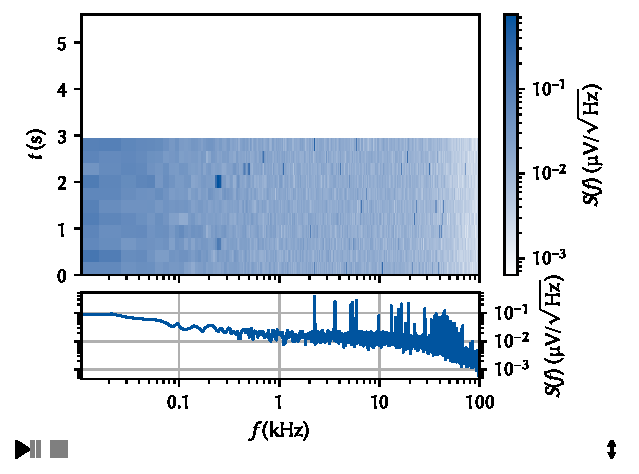
\includegraphics{pdf/spectrometer/live_view}
    \caption[Spectrometer live view]{
        Spectrometer live view.
        The bottom plot shows the most recently acquired spectrum, while the top plot shows a waterfall plot of the most recent ones.
        Data acquisition runs in a background thread, keeping the interpreter responsive and available to interact with instruments, for example.
        The icons in the bottom left and right corner allow interacting with the live view.
    }
    \label{fig:speck:software:live_view}
\end{figure}


\pagelayout{wide} % No margins
\addpart{Characterization and Improvements of a Millikelvin Confocal Microscope}\label{part:setup}
\pagelayout{margin} % Restore margins

\pagelayout{wide} % No margins
\addpart{Electrostatic Trapping of Excitons in Semiconductor Membranes}\label{part:measurements}
\pagelayout{margin} % Restore margins

\pagelayout{wide} % No margins
\addpart{A Filter-Function Formalism For Quantum Operations}\label{part:filter_functions}
\pagelayout{margin} % Restore margins

% mainfile: ../../main.tex
\chapter{Introduction}\label{ch:ff:introduction}
\begin{partcontribs}
    \Thispart is based to large extent on \sideciter{Hangleiter2021}, an early draft of which in turn was my Master's thesis~\sidecite{Hangleiter2019}, and as such contains text written by all three authors.
    \Cref{ch:ff:examples,sec:app:ff:time_domain_methods} additionally contains results published in \sideciter{Cerfontaine2021}.
    Parts of this work have also been included in \sideciter{Cerfontaine2019}.
    % TODO: can we make this nicer?
    Refer to References~\cite[Section 1.3]{Hangleiter2019} and~\cite[Section 3.7]{Cerfontaine2019} for detailed author contributions up to that point.
    \Cref{ch:ff:validation,sec:app:ff:concatenation} contain new results.
\end{partcontribs}
\begin{authornote}
    In Reference~\cite{Hangleiter2021}, extensive use was made of \citeauthor{Kubo1962}'s \emph{cumulant expansion}~\cite{Kubo1962}.
    Due to an error in \citeauthor{Kubo1962}'s paper which was only pointed out several years later~\cite{Fox1976} and we were not aware of, those results turned out to be not exact as claimed but approximate~\sidecite{Hangleiter2024}.\sidenote{
        Unfortunately, the error has proliferated through the literature and proves quite pervasive despite the significant amount of time that has passed since it was first discovered.
        Recent examples include~\citer{Norris2016}.
        One may only speculate if this is because of the 14 years that passed between the original publication and the correction, the lack of an erratum once the mistake had been discovered, or simply because of \citeauthor{Kubo1962}'s fame.
        In any case, it might serve as a cautionary tale and possibly an impetus to a less static publication system that allows, for example, cross-linking commentaries and critiques.
    }
    We address this discrepancy in \cref{ch:ff:validation}.
\end{authornote}
\AutoLettrine{In} the circuit model of quantum computing, computations are driven by applying time-local quantum gates.
Any algorithm can be compiled using sequences of one- and two-qubit gates~\cite{DiVincenzo1995}.
Ideal, error-free gates are represented by unitary transformations, so that simulating the action of an algorithm on an initial state of a quantum computer amounts to simple matrix multiplication.
Real implementations are subject to noise that causes decoherence resulting in gate errors.
If the noise is uncorrelated between gates, its effect can be described by quantum operations acting as linear maps on density matrices, even when several gates are concatenated.
A closely related approach is the use of a master equation in \gls{gksl} form~\cite{Gorini1976,Lindblad1976}, which governs the dynamics of density matrices under the influence of Markovian noise with a flat power spectral density.

Yet many physical systems used as hosts for qubits do not satisfy the condition of uncorrelated noise.
One example frequently encountered in solid-state systems is that of \oneoverf noise, which in principle contains arbitrarily long correlation times.
It emerges for instance as flux noise in superconducting qubits and electrical noise in quantum dot qubits~\cite{Brownnutt2015,Kumar2016a,Yoneda2018,Paladino2014}.
Whereas simple approaches exist to treat for example quasistatic noise, which corresponds to perfectly correlated noise (\ie, a spectrum with weight only at zero frequency), they cannot be applied to \oneoverf noise because of the wide distribution of correlation times it contains~\cite{Connors2022}.
Thus, there is a gap in the mathematical descriptions of gate operations for noises with arbitrary power spectra that exist between the extremal cases of perfectly flat (white) and sharply peaked (quasistatic) spectra.
To capture experimentally relevant effects important to understand the capabilities of quantum computing systems, a universally applicable formalism is hence desirable.
For example, one may expect the fidelity requirements for quantum error correction to be more stringent for correlated noise as errors of different gates can interfere constructively~\cite{Ng2009}.
On the other hand, it might also be possible to use correlation effects to one's benefit, attenuating decoherence by cleverly constructing the gate sequences in algorithms.

As experimental platforms begin to approach fidelity limits set by employing primitive pulse schemes~\cite{Veldhorst2014,Debnath2016,Yoneda2018} and detailed knowledge about noise sources and spectra in solid-state systems becomes available~\cite{Dial2013,Quintana2017,Malinowski2017}, control pulse optimizations tailored towards specific systems will be required to further push fidelities beyond the error correction threshold~\cite{Barends2014,Blume-Kohout2017}.
This calls for flexible and generically applicable tools as a basis for the numerical optimization of pulses as well as the detailed analysis of the quantum processes they effect.
In order to obtain a useful description also for gate operations that decouple from leading orders of noise, such as \glspl{dcg}~\cite{Khodjasteh2009}, beyond leading order results are required.

In \citer{Cerfontaine2021} we presented a formalism based on filter functions and the \gls{me} that addresses these needs and limitations of the canonical master equation approach for correlated noise.
Specifically, we showed how process descriptions can be obtained perturbatively for arbitrary classical noise spectra and derived a concatenation rule to obtain the filter function of a sequence of gates from those of the individual gates.
This work generalizes and extends these results.

\Glspl{ff} were originally introduced to describe the decay of phase coherence under \gls{dd} sequences~\cite{Kofman2001,Martinis2003,Uhrig2007,Cywinski2008} consisting of wait times and perfect $\pi$-pulses.
The formalism facilitated recognizing these sequences as band-pass filters that allow for probing the environmental noise characteristics of a quantum system through noise spectroscopy~\cite{Alvarez2011,Bylander2011,Paz-Silva2017,Malinowski2017} or optimizing sequences to suppress specific noise bands~\cite{Biercuk2009,Uys2009,Soare2014,Malinowski2017}.
It can also be extended to fidelities of gate operations for single~\cite{Green2012,Green2013} or multiple~\cite{Gungordu2018,Ball2020} qubits using the \gls{me}~\cite{Magnus1954,Blanes2009} as well as more general \gls{dd} protocols~\cite{Paz-Silva2014}.
The works by~\citet{Green2013} and~\citet{Clausen2010} also introduced the notion of the control matrix as a quantity closely related to the canonical filter function that is convenient for calculations.
In this context, the formalism's capability to predict fidelities of gate implementations has been identified and experimentally tested~\cite{Green2013,Kabytayev2014,Soare2014,Ball2016}.
More recently, it has also proved useful in assessing the performance requirements for classical control electronics~\cite{VanDijk2019}.

While analytical approaches allow for the calculation of filter functions of arbitrary quantum control protocols in principle, it is in practice often a tedious task to determine analytical solutions to the integrals involved if the complexity of the applied wave forms goes beyond simple square pulses or extends to multiple qubits.
Moreover, one does not always have a closed-form expression of the control at hand, such as is the case for numerically optimized control pulses.
This calls for a numerical approach which, while giving up some of the insights an analytical form offers, is universally applicable and eliminates the need for laborious analytical calculations.

Here, we build and extend upon our work of~\citer{Cerfontaine2021} and that of~\citer{Green2013} to show that the formalism can be recast within the framework of stochastic Liouville equations by means of the cumulant expansion~\cite{Kubo1962,Kubo1963,Fox1976,Bianucci2020}.
For Gaussian noise commuting with the control, this entails exact results for the quantum process of an arbitrary control operation using only first and second order terms of the \gls{me}~\cite{Magnus1954}.
If the noise is Gaussian but in general non-commuting, the cumulant expansion does not terminate~\cite{Fox1976}, but we show that the truncation still yields highly accurate results except in the ultralow-frequency regime by computing the exact filter function from random sampling.
Moreover, due to the fact that the \gls{me} retains the algebraic structure of the expanded quantity~\cite{Blanes2009} we are able to separate incoherent and coherent contributions to the quantum process.
We give explicit methods to evaluate these terms for piecewise-constant control pulses.
Moreover, we show that the formalism naturally lends itself as a tool for numerical calculations and present the \filterfunctions \python software package that enables calculating the filter function of arbitrary, piecewise constant defined pulses~\cite{Hangleiter_ff}.
On top of providing methods to handle individual quantum gates, the package also implements the concatenation operation as well as parallelized execution of pulses on different groups of qubits, allowing for a highly modular and hence computationally powerful treatment of quantum algorithms in the presence of correlated noise.
Given an arbitrary, classical noise spectral density, it can be used to calculate a matrix representation of the error process.
From this matrix one can extract average gate fidelities, transition probabilities, and leakage rates as we derive below.
To simplify adaptation the software's \gls{api} is strongly inspired by and compatible with \qutip~\cite{Johansson2012} as well as \qopt~\cite{Teske2022}.
This allows users to use these packages in conjunction.
Assessing the computational performance, we show that our method outperforms \gls{mc} simulations for single gates.
New analytical results applicable to periodic Hamiltonians and employing the concatenation property make this advantage even more pronounced for sequences of gates.
To highlight the main software features, we show example applications below.

We provide this package in the expectation that it will be a useful tool for the community.
Besides recasting and expanding on our earlier introduction of the formalism in~\citer{Cerfontaine2021}, the present work is intended to provide an overview of the software and its capabilities.
It is structured as follows: In \cref{ch:ff:theory} we derive a closed-form expression for unital quantum operations in the presence of non-Markovian Gaussian noise and lay out how it may be evaluated using the filter-function formalism.
We review the concatenation of quantum operations shown in~\citer{Cerfontaine2021} and furthermore adapt the method by~\citet{Green2013} to calculate the filter function of an arbitrary control sequence numerically.
We will specifically focus on computational aspects of the formalism and lay out how to compute various quantities of interest.
Moreover, we classify its computational complexity for calculating average gate fidelities and remark on simplifications that allow for drastic improvements in performance in certain applications.
In \cref{ch:ff:validation}, we validate the truncation of the cumulant expansion after the second order using a random sampling approach to compute the exact filter functions of the noisy quantum process for Gaussian noise.
In \cref{ch:ff:software}, we then introduce the \filterfunctions software package by outlining the programmatic structure and giving a brief overview over the \gls{api}.
Lastly, in \cref{ch:ff:examples}, we show the application of the software by means of four examples that highlight various features of the formalism and its implementation.
Therein, we first demonstrate that the formalism can predict average gate fidelities for complex two-qubit quantum gates in agreement with computationally much more costly \gls{mc} calculations.
Next, we show how it can be applied to periodically driven systems to efficiently analyze Rabi oscillations.
We finally establish the formalism's ability to predict deviations from the simple concatenation of unitary gates for sequences and algorithms in the presence of correlated noise by simulating a \gls{rb} experiment as well as assembling a \gls{qft} circuit from numerically optimized gates.
We conclude by briefly remarking on possible future application and extension of our method in \cref{ch:ff:conclusion}.

Throughout this part we will denote Hilbert-space operators by Roman font, \eg $U$, and quantum operations and their representations as transfer matrices in Liouville space by calligraphic font, \eg \liouvU, which we also use for the control matrix \ctrlmat to emphasize its innate connection to a transfer matrix.
For consistency, a unitary quantum operation will share the same character as the corresponding unitary operator.
An operator in the interaction picture will furthermore be designated by an overset tilde, \eg $\tilde{H} = U\adjoint H U$ with $U$ the unitary operator defining the co-moving frame.
Definitions of new quantities on the left and right side of an equality are denoted by $\coloneqq$ and $\eqqcolon$, respectively.
We use a central dot ($\placeholder$) as a placeholder in some definitions of abstract operators such as the Liouvillian, denoted by $\mc{L}\coloneqq\comm{H}{\placeholder}$, which is to be understood as the commutator of the corresponding Hamiltonian $H$ and the operator that $\mc{L}$ acts on.
The identity matrix is denoted by \eye and its dimension always inferred from context.
Furthermore, we will use Greek letters for indices that correspond to noise operators in order to distinguish them clearly from those that correspond to basis or matrix elements.
Lastly, we work in units where $\hbar =  1$.

% mainfile: ../../main.tex
\chapter{Monte Carlo and Lindblad master equation simulations}\label{ch:ff:time_domain_methods}
\section{Validation of QFT fidelities}\label{sec:ff:time_domain_methods:qft_validation}
In this section, we perform Lindblad master equation and \gls{mc} simulations to verify the fidelities predicted for the \gls{qft} circuit in the main text.
We focus on noise exclusively on the third qubit, entering through the noise operator $B_\alpha\equiv\sigma_y\gth{3}$.

To validate the fidelity for white noise, we use a Lindblad master equation~\cite{Lindblad1976,Gorini1976} in superoperator form.
We represent linear maps $\mc{A}: \rho\rightarrow\mc{A}(\rho)$ by matrices in the Pauli transfer matrix representation as (see \citer{Hangleiter2021} for more details)
\begin{equation}
    \mc{A}_{ij} \coloneqq \tr(\sigma_i\mc{A}(\sigma_j))
\end{equation}
and operators as column vectors (\ie, generalized Bloch vectors) as
\begin{equation}\label{eq:ff:bloch_vector}
    \rho_i \coloneqq \tr(\sigma_i\rho),
\end{equation}
allowing us to write the Lindblad equation
\begin{equation}\label{eq:ff:lindblad:hilbert}
\dv{t}\rho(t) = -\i\comm{H(t)}{\rho(t)} + \sum_\alpha \gamma_\alpha\left(L_\alpha\rho(t) L_\alpha\adjoint - \frac{1}{2}\acomm{L_\alpha\adjoint L_\alpha}{\rho(t)}\right)
\end{equation}
as a linear differential equation in matrix form,
\begin{equation}\label{eq:ff:lindlbad:liouville}
\dv{t}\rho_i(t) = \sum_j\left(-\i\mc{H}_{ij}(t)+ \sum_\alpha \gamma_\alpha \mc{D}_{\alpha, ij}\right)\rho_j(t).
\end{equation}
Here, $\mc{H}_{ij}(t) = \tr(\sigma_i\comm{H(t)}{\sigma_j})$ and $\mc{D}_{\alpha, ij} = \tr(\sigma_i L_\alpha\sigma_j L_\alpha\adjoint - \frac{1}{2}\sigma_i \acomm{L_\alpha\adjoint L_\alpha}{\sigma_j})$.
By setting $L_\alpha\equiv\sigma_y\gth{3}$ as well as $\gamma_\alpha\equiv\flatfrac{S_0}{2}$ with $S_0$ the amplitude of the one-sided noise \gls{psd} so that $S(\omega) = S_0$, we can compare the fidelity obtained from the filter functions to that from the explicit simulation of \cref{eq:ff:lindlbad:liouville}.
The latter is computed as $\avgfid = d^{-2}\tr(\mc{Q}\adjoint\mc{U})$, where $\mc{Q}$ is the superpropagator due to the Hamiltonian evolution alone (\ie, the ideal evolution without noise).

For the Monte Carlo simulation, we explicitly generate time traces of $b_Q(t)$ (\cf \cref{eq:ff:noise_hamiltonian}) by drawing pseudo-random numbers from a distribution whose \gls{psd} is $S(f) = \flatfrac{S_0}{f}$.
To do this, we draw complex, normally distributed samples in frequency space (\ie white noise), scale it with the square root of the \gls{psd}, and finally perform the inverse Fourier transform.
We choose an oversampling factor of 16 so that the time discretization of the simulation is $\Delta t_\mr{MC} = \flatfrac{\Delta t}{16} = \qty{62.5}{\pico\second}$ ($\Delta t = \qty{1}{\nano\second}$ is the time step of the pulses used in the FF simulation), leading to a highest resolvable frequency of $\fmax = \qty{16}{\giga\hertz}$.
Conversely, we increase the frequency resolution by sampling a time trace longer by a given factor, giving frequencies below \fmin (\qty{16}{\kilo\hertz} for pink, \qty{0}{\hertz} for white noise) weight zero, and truncating it to the number of time steps in the algorithm times the oversampling factor.
This yields a time trace with frequencies $f\in [\fmin, \fmax]$ and a given resolution (we choose $\df = \qty{160}{\hertz}$).

We then proceed to diagonalize the Hamiltonian $H(t) = H_c(t) + H_n(t)$ and compute the propagator for one noise realization as
\begin{equation}\label{eq:ff:mc_propagator}
U(t) = \prod_g V\gth{g}\exp\lbrace -\i\Omega\gth{g}\Delta t_\mr{MC}\rbrace V^{(g)\dagger},
\end{equation}
where $V\gth{g}$ is the unitary matrix of eigenvectors of $H(t)$ during time segment $g$ and $\Omega\gth{g}$ the diagonal matrix of eigenvalues.
Finally, we obtain an estimate for the average gate fidelity \avgfid from the entanglement fidelity \entfid as
\begin{equation}
    \ev{\avgfid} = \ev{\frac{d\entfid + 1}{d+1}} = \ev{\frac{\abs{\tr(Q\adjoint U(\tau))}^2 + d}{d(d+1)}}.
\end{equation}
Here, $Q\equiv\Uc(t=\tau)$ is the noise-free propagator at time $\tau$ of completion of the circuit and $\ev{\placeholder}$ denotes the ensemble average over $N$ Monte Carlo realizations of \cref{eq:ff:mc_propagator}, \ie, $\ev{A}=N\inverse\sum_{i=1}^N A_i$.
The standard error of the mean can be obtained as $\sigma_{\ev{\avgfid}} = \sigma_{\avgfid} / \sqrt{N}$ with $\sigma_{\avgfid}$ the standard deviation over the Monte Carlo traces.

% mainfile: ../../main.tex
\chapter{Filter functions from random sampling}\label{ch:ff:validation}
\AutoLettrine{In} our derivation of the average error map \liouvUeavg, \cref{eq:ff:cumulant_expansion}, we employed the cumulant expansion due to \citet{Kubo1962,Kubo1963}.
In his papers, \citeauthor{Kubo1962} makes the claim that this expansion is exact for Gaussian noise when truncating after the second order, even for \emph{$q$-numbers}, \ie, linear operators.
For \emph{$c$-numbers} -- scalars -- this is a well-known result in statistics; the Gaussian probability distribution is fully described by its first two cumulants, the mean $\mu$ and variance $\sigma^2$.
However, \citet{Fox1976} showed many years later that \citeauthor{Kubo1962}'s claim for $q$-numbers does not hold, and that non-commutativity in the Gaussian variables can cause higher-order cumulants to not vanish.
There are two limiting cases in which the expansion remains exact; first, for white noise, whose auto-correlation function is singular at $t=0$, and thus \enquote{decouples} higher-order cumulants, and second, commuting noise, for which $\comm{\Hc(t)}{\Hn(t)} = 0\forall t$.
Beyond these two cases, we must therefore assume that the map given by \cref{eq:ff:cumulant_expansion} is merely approximate when including only up to second-order terms from the Magnus expansion.\sidenote{
    Note that the cluster property still holds in all cases, and hence for Gaussian noise only even-order cumulants do not vanish~\cite{VanKampen1974,VanKampen1974a,Fox1976,Bianucci2020}.
}
In this chapter, we investigate the extent of this error.
To this end, we compute the \emph{exact} \acrfull{ff} using a \acrfull{mc} approach by randomly sampling monochromatic noise fields.

\section{Reconstruction by frequency-comb time domain simulation}\label{sec:ff:validation:method}
For a given interaction-picture quantum operation \liouvUetavg resulting from the quantum system's evolution under the noise fully characterized by its \gls{psd} $S(\omega)$, we \emph{define} the filter function \FFot by
\begin{align}\label{eq:ff:filter_function:definition}
    \liouvUetavg = \exp\cumulantfun(\tau) = \exp\left\{-\int\frac{\dd{\omega}}{2\pi}\FFot S(\omega)\right\}.
\end{align}
Now, suppose that
\begin{equation}\label{eq:ff:psd:monochromatic}
    S(\omega) = 2\pi\sigma_i^2 \delta(\omega - \omega_i) \eqqcolon S_i(\omega),
\end{equation}
that is, the \gls{psd} of a monochromatic sinusoid of frequency $\omega_i$ and \gls{rms} $\sigma_i$.\sidenote{
    \Cref{eq:ff:psd:monochromatic} discretizes $S(\omega)$ by sampling it at points $\omega_i$, \ie,
    \begin{align*}
        S(\omega) \sim \lim_{n\to\infty}\sum_{i=1}^n S_i(\omega).
    \end{align*}
    See also \cref{sidenote:continuum_limit}.
}
\Cref{eq:ff:filter_function:definition} then becomes
\begin{align}
    \ev*{\liouvUe_i(\tau)} \coloneqq \liouvUetavg =& \exp\left\lbrace -2\pi\sigma_i^2\int\frac{\dd{\omega}}{2\pi}\FFot\delta(\omega - \omega_i)\right\rbrace \\
                                                  =& \exp\left\lbrace -\sigma_i^2\mc{F}(\omega_i;\tau)\right\rbrace, \label{eq:ff:filter_function:monochromatic}
\end{align}
where $\ev*{\liouvUe_i(\tau)}$ is the noisy quantum operation generated by monochromatic noise with \gls{psd} $S_i(\omega)$ according to \cref{eq:ff:psd:monochromatic}.
It is now easy to invert \cref{eq:ff:filter_function:monochromatic}, and we obtain
\begin{align}\label{eq:ff:filter_function:monochromatic:solved}
    \mc{F}(\omega_i; \tau) = -\sigma_i^{-2}\log\ev*{\liouvUe_i(\tau)}.
\end{align}
Because we represent quantum operations as matrices in Liouville space, \cref{eq:ff:filter_function:monochromatic:solved} is straightforward to implement on a computer; to sample the exact \gls{ff} at the set of discrete frequencies $\lbrace\omega_i\rbrace_i$ we simply need to compute $\ev*{\liouvUe_i(\tau)}$  using a time-domain simulation method of our choice and take the logarithm!\sidenote{A similar approach was pursued by \citeauthor{Geck2021} in her PhD thesis to compare gate fidelities~\cite{Geck2021}.}

Indeed, we can go a step further and split apart the coherent and incoherent contributions to the noisy evolution.
Since (in-)coherent quantum operations are represented by (anti-)symmetric matrices in Liouville space, we may define the incoherent and coherent \glspl{ff} by
\begin{equation}\label{eq:ff:filter_function:monte_carlo:incoherent}
    \begin{split}
        \mc{F}_\decayamps(\omega_i;\tau) =& \frac{1}{2}\left(\mc{F}(\omega_i;\tau) + \mc{F}(\omega_i;\tau)\transpose\right) \\
                                         =& \frac{1}{2\sigma_i^2}\left(\log\ev*{\liouvUe_i(\tau)} + \log\ev*{\liouvUe_i(\tau)}\transpose\right),
    \end{split}
\end{equation}
and
\begin{equation}\label{eq:ff:filter_function:monte_carlo:coherent}
    \begin{split}
        \mc{F}_\freqshifts(\omega_i;\tau) =& \frac{1}{2}\left(\mc{F}(\omega_i;\tau) - \mc{F}(\omega_i;\tau)\transpose\right) \\
                                          =& \frac{1}{2\sigma_i^2}\left(\log\ev*{\liouvUe_i(\tau)} - \log\ev*{\liouvUe_i(\tau)}\transpose\right),
    \end{split}
\end{equation}
respectively.
In the filter-function formalism presented in \cref{ch:ff:theory}, \cref{eq:ff:filter_function:monte_carlo:coherent,eq:ff:filter_function:monte_carlo:incoherent} correspond -- up to corrections from non-vanishing higher cumulants -- to linear combinations of the generalized filter functions from second and first order Magnus expansion, respectively.
To be more precise, let us again consider \cref{eq:ff:cumulant:truncated:liouville}.
Rather than first performing the integrations of \cref{eq:ff:frequency_shifts:time,eq:ff:decay_amplitudes:time} to obtain the decay amplitudes \decayamps and frequency shifts \freqshifts, and then the contractions with the trace tensor functions $g_{ijkl}$ and $f_{ijkl}$, first contract the latter with the control matrices to obtain the time-domain filter functions\sidenote{
    We consider a single noise operator and drop the index for brevity.
}
\begin{align}
    \FF\gth{\decayamps}_{ij}(t_1, t_2) &= \frac{1}{2}\sum_{kl} g_{ijkl}\ctrlmat_{k}(t_1)\ctrlmat_{l}(t_2), \label{eq:ff:filter_function:cumulant:incoherent}\\
    \FF\gth{\freqshifts}_{ij}(t_1, t_2) &= \frac{1}{2}\sum_{kl} f_{ijkl}\ctrlmat_{k}(t_1)\ctrlmat_{l}(t_2). \label{eq:ff:filter_function:cumulant:coherent}
\end{align}
Again moving to Fourier space and following the same procedure as in \cref{sec:ff:theory:decay_amplitudes,sec:ff:theory:frequency_shifts} leads to the coherent and incoherent frequency-domain filter functions $\FF\gth{\decayamps}_{kl}(\omega;\tau)$ and $\FF\gth{\freqshifts}_{kl}(\omega;\tau)$ that we must simply integrate over to obtain the average error process \liouvUetavg,\sidenote{
    That is, we have $\FF\gth{\freqshifts}_{ij}(\omega;\tau) = 1/2\sum_{kl}f_{ijkl}\FF\gth{2}_{kl}(\omega;\tau)$ with the latter defined in \cref{eq:ff:frequency_shifts:filter_function} as well as $\FF\gth{\decayamps}_{ij}(\omega;\tau) = 1/2\sum_{kl}g_{ijkl}\FF_{kl}(\omega;\tau)$ with the latter defined in \cref{eq:ff:filter_function:generalized}.
}
\begin{equation}\label{eq:ff:filter_function:cumulant:total}
    \liouvUetavg = \exp\left\lbrace -\int\ddf{\omega}S(\omega)\left[\FF\gth{\decayamps}(\omega;\tau) + \FF\gth{\freqshifts}(\omega;\tau)\right]\right\rbrace.
\end{equation}
This allows us to analyze in detail deviations of the closed-form expression obtained by means of the cumulant expansion, \cref{eq:ff:filter_function:cumulant:total}, from the exact filter function sampled at discrete $\omega_i$ by \cref{eq:ff:filter_function:monochromatic:solved}.
In the following, we will lay out explicitly how the latter can be computed in the time domain using a \gls{mc} method.\sidenote{
    See also \cref{sec:app:ff:time_domain_methods} for details on the \gls{mc} method.
}

To begin with, observe that
\begin{align}
    \expval*{\liouvUe_i(\tau)} = \liouvQ\transpose \expval*{\liouvU_i(\tau)},
\end{align}
where as usual \liouvQ is the complete superpropagator of the noise-free time evolution and $\liouvU_i(\tau)$ that of the noisy time evolution generated by a single realization of the noise $b(t)$, both of which are unitary.
In \gls{mc}, we generate $N$ realizations of this noise process in the time domain, compute the full time evolution superpropagator $\liouvU_i(\tau)$, and then evaluate the expectation value $\expval{\placeholder}$ as the ensemble average to obtain $\ev*{\liouvU_i(\tau)}$.\sidenote[][*-8]{
    For $N$ realizations of the stochastic process underlying $b(t)$, the ensemble average of a quantity $A(t)$ that is a function of $b(t)$ is given by
    \begin{align*}
        \expval{A}(t) = \frac{1}{N}\sum_{i=1}^N A_i(t)
    \end{align*}
    where $i$ enumerates the realizations of the stochastic process.
    The relative error of this average scales as $N^{-\flatfrac{1}{2}}$.
}
Inserting into \cref{eq:ff:filter_function:monochromatic}, we find that
\begin{equation}\label{eq:ff:filter_function:monte_carlo}
    \mc{F}(\omega_i; \tau) = \sigma_i^{-2}\log\expval*{\liouvUe_i(\tau)} = \sigma_i^{-2}\log\liouvQ\transpose\expval{\liouvU_i(\tau)}.
\end{equation}
If we evaluate \cref{eq:ff:filter_function:monte_carlo} for a set of frequencies $\lbrace\omega_i\rbrace_i$ sampling the true spectrum $S(\omega)$ sufficiently well, we thus obtain the exact filter function \FFot (within the accuracy of \gls{mc}), allowing us to compare the accuracy of the formalism developed in \cref{ch:ff:theory}.

So what does a single noise realization of \cref{eq:ff:psd:monochromatic} in the time domain look like?
It is a sinusoid with amplitude $A_i \sim\rayleigh(\sigma_i)$,\sidenote{
    $\rayleigh(\sigma)$ is the Rayleigh distribution with probability density function \cite{RayleighDistributionWiki}
    \begin{equation*}
        \rho(x) = \frac{x}{\sigma^2}\exp{-\frac{x^2}{2\sigma^2}}.
    \end{equation*}
    It describes the probability distribution of the distance from the origin of a point drawn from a bivariate normal distribution with mean $0$ and standard deviation $\sigma$.
}
frequency $\omega_i$, and phase $\phi \sim \uniform(0, 2\pi)$,\sidenote{
    The probability density function of the uniform distribution $\uniform(a, b)$ is
    \begin{equation*}
        \rho(y) = \begin{cases}
        (b - a)^{-1}    & \qif* a\leq y < b, \\
        0               & \qelse*
        \end{cases}
    \end{equation*}
}
\begin{equation}\label{eq:ff:monte_carlo:noise_trace}
    b(t) = A_i\sin(\omega_i t + \phi).
\end{equation}
To obtain the \gls{mc} estimate of \liouvUetavg, we therefore draw $N$ noise traces according to \cref{eq:ff:monte_carlo:noise_trace}, solve the Schrödinger equation, and finally perform the ensemble average from which we can deduce the filter function using \cref{eq:ff:filter_function:monte_carlo}.
From the spread of the individual \gls{mc} samples we obtain confidence intervals on the mean of the error transfer matrix by bootstrapping, which we propagate to the filter function by taking the Fréchet derivative of the matrix logarithm in \cref{eq:ff:filter_function:monte_carlo}~\cite{Al-Mohy2013}.

\section{Case studies}\label{sec:ff:validation:examples}
\begin{figure}
    \centering
    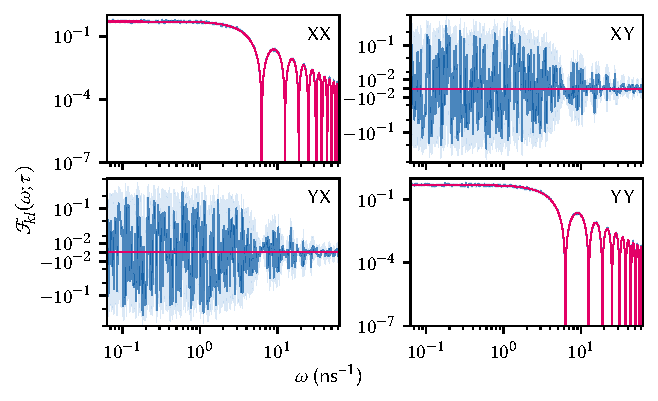
\includegraphics{img/pdf/filter_functions/monte_carlo_FF_Z}
    \caption[\imgsource{img/py/filter_functions/monte_carlo_filter_functions.py}]{
        Non-zero components of the \gls{ff} in the Pauli basis $\mathsf{P}_1$ for the pure dephasing Hamiltonian in \cref{eq:ff:validation:examples:z}.
        Magenta lines are from the cumulant expansion, \cref{eq:ff:filter_function:cumulant:total}, blue lines the mean of the \gls{mc} simulation, \cref{eq:ff:filter_function:monte_carlo}, and light blue shaded areas the \qty{95}{\percent} confidence interval.
        The diagonal elements (XX and YY) agree within the \gls{mc} confidence intervals, with the zeros at $2\pi n/\tau, n\in\{1,2,\dotsc\}$ agreeing down to \num{1e-15} where we can expect numerical errors to be limiting.
        The off-diagonal elements are quite noisy in the \gls{mc} simulation, but fluctuate about the expected value of zero.
    }
    \label{fig:ff:monte_carlo:Z}
\end{figure}

Let us now turn to applying the method to a few select case studies.
First, we consider a pure-dephasing Hamiltonian with
\begin{equation}\label{eq:ff:validation:examples:z}
    \begin{split}
        \Hc(t) &= \Omega\frac{\sz}{2}, \\
        \Hn(t) &= b(t)\frac{\sz}{2}.
    \end{split}
\end{equation}
Specifically, we let the system evolve under the Hamiltonian in \cref{eq:ff:validation:examples:z} for $\tau = \pi/\Omega$ to undergo a $\pi$-rotation around the $z$-axis of the Bloch sphere.
For this model, we expect the cumulant expansion to terminate after the second order because control and noise commute, and hence the interaction-picture noise Hamiltonian, $\Hnt(t)$, always commutes with itself, and therefore the filter-function formalism of \cref{ch:ff:theory} should give the exact result.
\Cref{eq:ff:validation:examples:z} can be solved analytically, and gives rise to an ideal dephasing channel whose \gls{ptm} representation is diagonal, $\liouvUetavg = \diag(1, 1-p, 1-p, 1)$ with $p$ the dephasing probability whose precise value depends on the form of the \gls{psd} $S(\omega)$.
Accordingly, the \gls{ff} $\FF_{kl}(\omega;\tau)$ should be zero everywhere but at $k=l\in\{1, 2\}\equiv\{x, y\}$ for the Pauli basis $\mathsf{P}_1$.
\Cref{fig:ff:monte_carlo:Z} shows the total \enquote{error transfer matrix filter functions} (\cref{eq:ff:filter_function:cumulant:total,eq:ff:filter_function:monte_carlo}) computed with both methods; magenta for the cumulant expansion and blue for the exact \gls{mc} method.
The diagonals agree perfectly within the confidence intervals, while the off-diagonals are dominated by numerical noise in the \gls{mc} approach.
Since the off-diagonals are zero, only the first-order Magnus terms contribute.\sidenote{
    Recall that $\FF\gth{\Delta}(\omega;\tau)$ is anti-symmetric.
}

\begin{figure*}
    \centering
    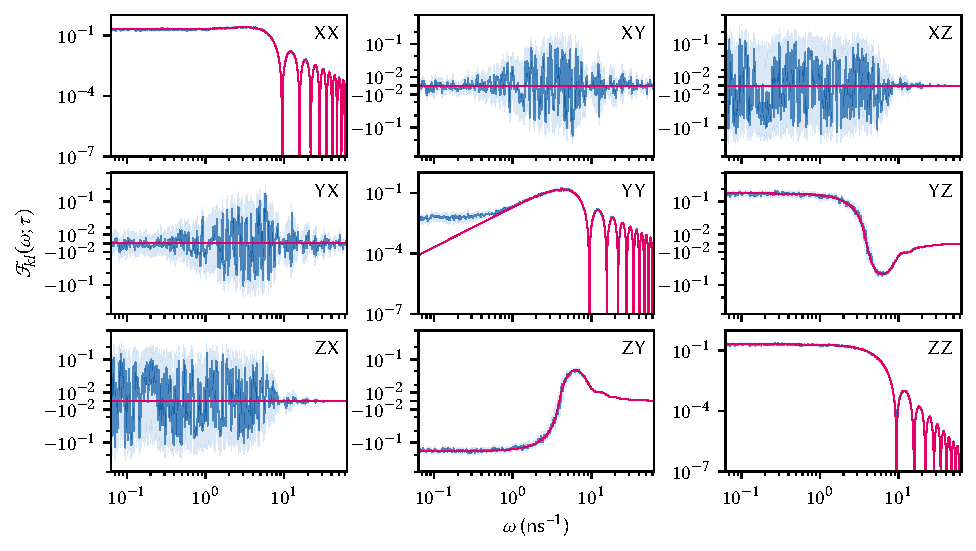
\includegraphics{img/pdf/filter_functions/monte_carlo_FF_X}
    \caption[\imgsource{img/py/filter_functions/monte_carlo_filter_functions.py}]{
        \Glspl{ff} for the non-commuting Hamiltonian in \cref{eq:ff:validation:examples:x}.
        Cumulant expansion calculation is shown in magenta, \gls{mc} in blue with light blue shaded areas the confidence intervals.
        Again, the nominally-zero off-diagonals are susceptible to numerical noise in the \gls{mc} method.
        The YY- and ZZ-terms show a deviation of the cumulant expansion calculation, while all others, including the coherent YZ- and ZY-terms appear to be exact up to the numerical uncertainty.
    }
    \label{fig:ff:monte_carlo:X}
\end{figure*}

The opposite extreme to the pure-dephasing Hamiltonian is obtained when changing the control to be transverse to the noise,
\begin{equation}\label{eq:ff:validation:examples:x}
    \begin{split}
        \Hc(t) &= \Omega\frac{\sx}{2}, \\
        \Hn(t) &= b(t)\frac{\sz}{2}.
    \end{split}
\end{equation}
In this case, control and noise Hamiltonian maximally do not commute at any time ($\Hnt(t)=\sz\cos\Omega t +\i\sy\sin\Omega t$) and we should expect the largest deviations from the exact filter functions in the approximation by truncating the cumulant function after the second order.
\Cref{fig:ff:monte_carlo:X} shows the \gls{ff} for a $\pi$-rotation around the $x$-axis of the Bloch sphere (\ie, $\tau = \pi/\Omega$ once again).
This time, all diagonal elements are nonzero, and the YY-term ($\FF_{22}(\omega;\tau)$ with $\sigma_2\equiv\sy$) displays a deviation between cumulant expansion and \gls{mc} simulation towards low frequencies!
This is exactly what we would expect according to \citet{Fox1976}, namely that the more correlated the noise is, the larger contributions from higher orders will be.\sidenote{
    Quasistatic noise is perfectly correlated---it assumes a single value for all times.
}
Also deviating is the ZZ-term, although not towards DC but where the filter function computed from the approximated cumulant function drops to zero.
By contrast, the XX-term shows good agreement between both methods.
Finally, two non-diagonal elements are nonzero, YZ and ZY, anti-symmetric terms which arise from the second-order Magnus and incur coherent errors.
For these, the cumulant approximation is excellent, showing no deviation within the confidence intervals.

\begin{figure*}
    \centering
    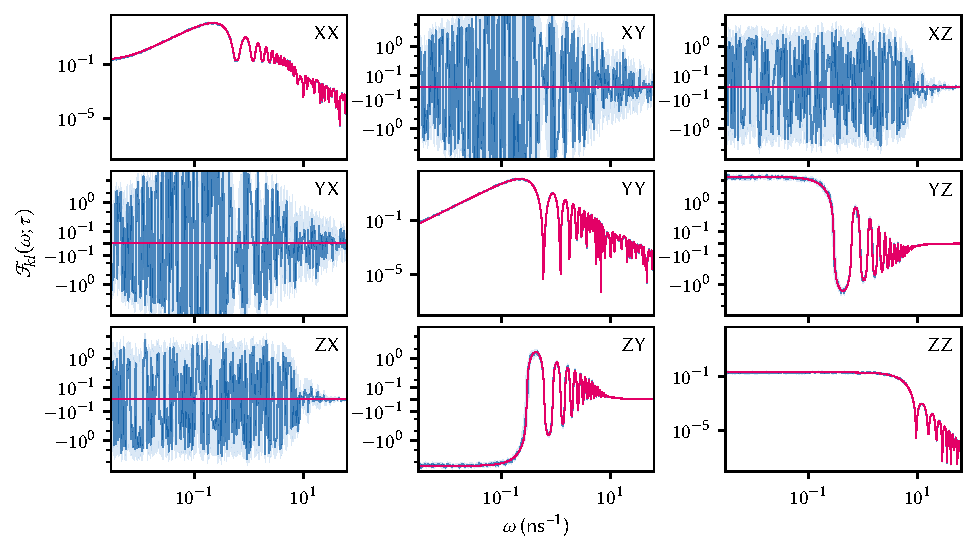
\includegraphics{img/pdf/filter_functions/monte_carlo_FF_spin_echo}
    \caption[\imgsource{img/py/filter_functions/monte_carlo_filter_functions.py}]{
        \Glspl{ff} for the \gls{se} Hamiltonian in \cref{eq:ff:validation:examples:se}.
        Cumulant expansion calculation is shown in magenta, \gls{mc} in blue with light blue shaded areas the confidence intervals.
        Both coherent and incoherent terms show excellent agreement between both methods.
    }
    \label{fig:ff:monte_carlo:se}
\end{figure*}

Finally, as a last example we consider the prototypical filter-function use case: the \acrfull{se}.
Here, the qubit idles for a time $\tau_{0}$ both before and after a $\pi$ rotation around the $x$-axis of the Bloch sphere, so that the Hamiltonian is given by
\begin{equation}\label{eq:ff:validation:examples:se}
    \begin{split}
        \Hc(t) &= \Omega(t)\frac{\sx}{2}, \\
        \Hn(t) &= b(t)\frac{\sz}{2},
    \end{split}
\end{equation}
with $\Omega(t) = \pi/\tau_\pi$ if $t\in[\tau_0, \tau_0+\tau_\pi]$ and zero else.
This pulse sequence is known to cancel quasistatic dephasing noise as the phase picked up on the equator of the Bloch sphere during the first period of free evolution is exactly cancelled by the phase picked up during the second period after the $\pi$-pulse.
Since the previous example demonstrated that the filter-function formalism based on the second-order cumulant expansion neglects contributions from higher orders in the case of transverse noise, we might expect the \gls{se} sequence to show similar behavior.
\Cref{fig:ff:monte_carlo:se} shows the results of the simulation.
The picture is similar -- albeit more complex -- to before, with nominally-zero terms suffering from numerical noise.
However, in contrast to the simple $\pi$-pulse Hamiltonian in \cref{eq:ff:validation:examples:x,fig:ff:monte_carlo:X}, the YY and ZZ terms show excellent agreement between the exact \gls{mc} method and the cumulant expansion.
We may speculate that the higher-order contributions not captured by the cumulant method in the previous case drop out due to the symmetry of the Hamiltonian.

In conclusion, we have developed a method to numerically compute the exact filter functions of the quantum process description of arbitrary Gaussian noise, and compared the thus obtained filter functions with those from the second-order truncation of the \gls{me} and cumulant expansions given in \cref{ch:ff:theory}.
The approach samples the Liouville-space filter function at discrete frequencies $\omega_i$ by simulating the unitary dynamics under monochromatic noise at that frequencies and averaging over the outcomes.
We found excellent agreement between the nominally exact and approximate methods in the case of commuting noise as well as the \gls{se} \gls{dd} sequence.
For non-commuting noise, we observed the expected deviation at very low frequencies that arises from non-vanishing higher order cumulants.

Rather than random sampling using \gls{mc}, this average could also be performed deterministically as the expectation value over the probability distributions governing $A_i$ and $\phi$,
\begin{equation}
    \mathbb{E}_{A_i,\phi}[\liouvU] = \int\dd{x}\rho_{A_i}(x)\int\dd{y}\rho_{\phi}(y)\liouvU[x, y],
\end{equation}
where we wrote $\liouvU[x, y]$ for the Liouville representation of the propagator for single $x$ and $y$ drawn from their respective distributions, and $\mathbb{E}_X[A]$ denotes the expectation value of an observable $A$ with respect to the random variable $X$ with probability density function $\rho_X$.
This technique allows the expectation value $\mathbb{E}[\liouvU]\equiv\ev{\liouvU}$ to be evaluated to arbitrary precision numerically, but is typically less efficient than \gls{mc}.
It would be interesting to see if the numerical noise observed in off-diagonal elements of the filter functions in \cref{fig:ff:monte_carlo:Z,fig:ff:monte_carlo:X,fig:ff:monte_carlo:se} persists with this method.

% ==================================================
%           INTRODUCTION SECTION
% ==================================================
\chapter{Introduction}\label{ch:ff:introduction}
In the circuit model of quantum computing, computations are driven by applying time-local quantum gates.
Any algorithm can be compiled using sequences of one- and two-qubit gates~\cite{DiVincenzo1995}.
Ideal, error-free gates are represented by unitary transformations, so that simulating the action of an algorithm on an initial state of a quantum computer amounts to simple matrix multiplication.
Real implementations are subject to noise that causes decoherence resulting in gate errors.
If the noise is uncorrelated between gates, its effect can be described by quantum operations acting as linear maps on density matrices, even when several gates are concatenated.
A closely related approach is the use of a Master equation in Lindblad form~\cite{Lindblad1976}, which governs the dynamics of density matrices under the influence of Markovian noise with a flat power spectral density.

Yet many physical systems used as hosts for qubits do not satisfy the condition of uncorrelated noise.
One example frequently encountered in solid state systems is that of \oneoverf noise, which in principle contains arbitrarily long correlation times.
It emerges for instance as flux noise in superconducting qubits and electrical noise in quantum dot qubits~\cite{Brownnutt2015,Kumar2016,Yoneda2018,Paladino2014}.
Whereas simple approaches exist to treat for example quasistatic noise, which corresponds to perfectly correlated noise (\ie, a spectrum with weight only at zero frequency), they cannot be applied to \oneoverf noise because of the wide distribution of correlation times it contains.
Thus, there is a gap in the mathematical descriptions of gate operations for noises with arbitrary power spectra that exist between the extremal cases of perfectly flat (white) and sharply peaked (quasistatic) spectra.
To capture experimentally relevant effects important to understand the capabilities of quantum computing systems, a universally applicable formalism is hence desirable.
For example, one may expect the fidelity requirements for quantum error correction to be more stringent for correlated noise as errors of different gates can interfere constructively~\cite{Ng2009}.
On the other hand, it might also be possible to use correlation effects to one's benefit, attenuating decoherence by cleverly constructing the gate sequences in algorithms.

As experimental platforms begin to approach fidelity limits set by employing primitive pulse schemes~\cite{Veldhorst2014,Debnath2016,Yoneda2018} and detailed knowledge about noise sources and spectra in solid-state systems becomes available~\cite{Dial2013,Quintana2017,Malinowski2017}, control pulse optimizations tailored towards specific systems will be required to further push fidelities beyond the error correction threshold~\cite{Barends2014,Blume-Kohout2017}.
This calls for flexible and generically applicable tools as a basis for the numerical optimization of pulses as well as the detailed analysis of the quantum processes they effect.
In order to obtain a useful description also for gate operations that decouple from leading orders of noise, such as \glspl{dcg}~\cite{Khodjasteh2009}, beyond leading order results are required.

In an accompanying publication~\cite{Cerfontaine2021} we presented a formalism based on filter functions and the \gls{me} that addresses these needs and limitations of the canonical master equation approach for correlated noise.
Specifically, we showed how process descriptions can be obtained perturbatively for arbitrary classical noise spectra and derived a concatenation rule to obtain the filter function of a sequence of gates from those of the individual gates.
This paper extends these results.

\Glspl{ff} were originally introduced to describe the decay of phase coherence under \gls{dd} sequences~\cite{Kofman2001,Martinis2003,Uhrig2006,Cywinski2008} consisting of wait times and perfect $\pi$-pulses.
The formalism facilitated recognizing these sequences as band-pass filters that allow for probing the environmental noise characteristics of a quantum system through noise spectroscopy~\cite{Alvarez2011,Bylander2011,Paz-Silva2017,Malinowski2017} or optimizing sequences to suppress specific noise bands~\cite{Biercuk2009,Uys2009,Soare2014,Malinowski2017}.
It can also be extended to fidelities of gate operations for single~\cite{Green2012,Green2013} or multiple~\cite{Gungordu2018,Ball2020} qubits using the \gls{me}~\cite{Magnus1954,Blanes2009} as well as more general \gls{dd} protocols~\cite{Paz-Silva2014}.
The works by~\citeauthor{Green2013} and~\citeauthor{Clausen2010} also introduced the notion of the control matrix as a quantity closely related to the canonical filter function that is convenient for calculations.
In this context, the formalism's capability to predict fidelities of gate implementations has been identified and experimentally tested~\cite{Green2013,Kabytayev2014,Soare2014,Ball2016}.
More recently, it has also proved useful in assessing the performance requirements for classical control electronics~\cite{VanDijk2019}.

While analytic approaches allow for the calculation of filter functions of arbitrary quantum control protocols in principle, it is in practice often a tedious task to determine analytic solutions to the integrals involved if the complexity of the applied wave forms goes beyond simple square pulses or extend to multiple qubits.
Moreover, one does not always have a closed-form expression of the control at hand, such as is the case for numerically optimized control pulses.
This calls for a numerical approach which, while giving up some of the insights an analytical form offers, is universally applicable and eliminates the need for laborious analytic calculations.

Here, we build and extend upon our accompanying work of~\citer{Cerfontaine2021} and that of~\citer{Green2013} to show that the formalism can be recast within the framework of stochastic Liouville equations by means of the cumulant expansion~\cite{Kubo1962,Kubo1963,Fox1976,Bianucci2020}.
For Gaussian noise commuting with the control, this entails exact results for the quantum process of an arbitrary control operation using only first and second order terms of the \gls{me}~\cite{Magnus1954}.
Moreover, due to the fact that the \gls{me} retains the algebraic structure of the expanded quantity~\cite{Blanes2009} we are able to separate incoherent and coherent contributions to the process.
We give explicit methods to evaluate these terms for piecewise-constant control pulses.
Moreover, we show that the formalism naturally lends itself as a tool for numerical calculations and present the \filterfunctions \python software package that enables calculating the filter function of arbitrary, piecewise constant defined pulses~\cite{Hangleiter_ff}.
On top of providing methods to handle individual quantum gates, the package also implements the concatenation operation as well as parallelized execution of pulses on different groups of qubits, allowing for a highly modular and hence computationally powerful treatment of quantum algorithms in the presence of correlated noise.
Given an arbitrary, classical noise spectral density, it can be used to calculate a matrix representation of the error process.
From this matrix one can extract average gate fidelities, transition probabilities, and leakage rates as we derive below.
To simplify adaptation the software's API is strongly inspired by and compatible with \qutip~\cite{Johansson2012} as well as \qopt~\cite{Teske2021,Teske2022}.
This allows users to use these packages in conjunction.
Assessing the computational performance, we show that our method outperforms Monte Carlo simulations for single gates.
New analytic results applicable to periodic Hamiltonians and employing the concatenation property make this advantage even more pronounced for sequences of gates.
To highlight the main software features, we show example applications below.

We provide this package in the expectation that it will be a useful tool for the community.
Besides recasting and expanding on our earlier introduction of the formalism in~\citer{Cerfontaine2021}, the present paper is intended to provide an overview of the software and its capabilities.
It is structured as follows: In \cref{ch:ff:theory} we derive a closed-form expression for unital quantum operations in the presence of non-Markovian Gaussian noise and lay out how it may be evaluated using the filter function formalism.
We review the concatenation of quantum operations shown in~\citer{Cerfontaine2021} and furthermore adapt the method by~\citeauthor{Green2013} to calculate the filter function of an arbitrary control sequence numerically.
We will specifically focus on computational aspects of the formalism and lay out how to compute various quantities of interest.
Moreover, we classify its computational complexity for calculating average gate fidelities and remark on simplifications that allow for drastic improvements in performance in certain applications.
In \cref{ch:ff:software}, we introduce the software package by outlining the programmatic structure and giving a brief overview over the API.
Lastly, in \cref{ch:ff:examples}, we show the application of the software by means of four examples that highlight various features of the formalism and its implementation.
Therein, we first demonstrate that the formalism can predict average gate fidelities for complex two-qubit quantum gates in agreement with computationally much more costly Monte Carlo calculations.
Next, we show how it can be applied to periodically driven systems to efficiently analyze Rabi oscillations.
We finally establish the formalism's ability to predict deviations from the simple concatenation of unitary gates for sequences and algorithms in the presence of correlated noise by simulating a \gls{rb} experiment as well as assembling a \gls{qft} circuit from numerically optimized gates.
We conclude by briefly remarking on possible future application and extension of our method in \cref{ch:ff:considerata}.

Throughout the paper we will denote operators by Roman font, \eg $U$, and quantum operations and their representations as transfer matrices by calligraphic font, \eg \liouvU, which we also use for the control matrix \ctrlmat to emphasize its innate connection to a transfer matrix.
For consistency, a unitary quantum operation will share the same character as the corresponding unitary operator.
An operator in the interaction picture will furthermore be designated by an overset tilde, \eg $\tilde{H} = U\adjoint H U$ with $U$ the unitary operator defining the co-moving frame.
Definitions of new quantities on the left and right side of an equality are denoted by $\coloneqq$ and $\eqqcolon$, respectively.
We use a central dot ($\placeholder$) as a placeholder in some definitions of abstract operators such as the Liouvillian, denoted by $\mc{L}\coloneqq\comm{H}{\placeholder}$, which is to be understood as the commutator of the corresponding Hamiltonian $H$ and the operator that $\mc{L}$ acts on.
The identity matrix is denoted by \eye and its dimension always inferred from context.
Furthermore, we will use Greek letters for indices that correspond to noise operators in order to distinguish them clearly from those that correspond to basis or matrix elements.
Lastly, we work in units where $\hbar =  1$.

% ==================================================
%           THEORY SECTION
% ==================================================
\chapter{Filter function formalism for unital quantum operations}\label{ch:ff:theory}
We begin the theoretical part of this article by showing how a superoperator matrix representation of the error process, the \enquote{error transfer matrix}, of a unital quantum operation can be computed from the control matrix of the pulse implementing the operation.
The control matrix relates the operators through which noise couples into the system to a set of basis operators in the interaction picture and we detail how it can be calculated in a relatively efficient manner for two different situations.
First, we consider a sequence of gates whose control matrices have been precomputed.
Second, we lay out how the control matrix can be obtained from scratch under the assumption of piecewise constant control, which is often convenient for approximating continuous pulse shapes.
Other wave forms can be dealt with analogously by solving the corresponding integrals.
We then move on to show how several quantities of interest can be extracted and present optimized strategies for computing the central objects of the formalism.

\section{Transfer matrix representation of quantum operations}\label{sec:ff:theory:transfer_matrix}
\subsection{Brief review of quantum operations and superoperators}
The quantum operations formalism provides a general framework for the description of open quantum systems~\cite{Kraus1983,Nielsen2011}.
It forms the mathematical basis for \gls{qpt}~\cite{Chuang1997,Poyatos1997} as well as \gls{gst}~\cite{Blume-Kohout2013,Greenbaum2015} and has also been extensively employed in the context of \gls{rb}~\cite{Magesan2012a,Kimmel2014}.
Several different representations of quantum operations exist.
While all of them are equivalent one typically chooses the most convenient for the problem at hand.
For an overview of the most commonly used representations see~\citer{Greenbaum2015} and for matrix representations in particular~\citer{Nambu2005} and the references therein.
In this work we employ the Liouville representation, to the best of our knowledge first formalized by~\citeauthor{Fano1957}, to profit from its simple properties under composition.
It is also known as the transfer matrix representation and we will use the terms interchangeably below.
We now briefly review the concept and refer the reader to the literature for further details.
Concretely, the Liouville representation of an operation $\qp: \rho\rightarrow\qp(\rho)$ acting on density operators in a Hilbert space \Hspace of dimension $d$ is given by
\begin{equation}\label{eq:ff:liouville_representation}
    \qp_{ij}\doteq\tr(C_i\adjoint\qp(C_j))
\end{equation}
with an operator basis $\basis=\lbrace C_0, C_1, \dotsc, C_{d^2-1}\rbrace$ for the space of linear operators over \Hspace, $\mathsf{L}(\Hspace)$, orthonormal with respect to the Hilbert-Schmidt product $\dotHS{A}{B}\coloneqq\tr(A\adjoint B)$.
In the case that the operator basis corresponds to the Pauli matrices \cref{eq:ff:liouville_representation} is known as the Pauli transfer matrix (PTM).
The operation \qp is thus associated with a $d^2\times d^2$ matrix in \emph{Liouville space} \Lspace that describes its action as the degree to which the $j$ basis element is mapped onto the $i$th.
On \Lspace one can identify a set of basis kets $\lbrace\dket{C_i}\rbrace_{i=0}^{d^2-1} = \lbrace\dket{i}\rbrace_{i=0}^{d^2-1}$ isomorphic to the operators $C_i$ (and correspondingly bras $\dbra{i}$ to the adjoint $C_i\adjoint$) as well as the inner product $\dip{i}{j} = \dotHS{C_i}{C_j}$.
As the vectors $\dket{i}$ form an orthonormal basis, any operator on \Hspace can be written as a vector on \Lspace, $\dket{A} = \sum_i\dket{i}\dip{i}{A}$, whereas a superoperator on \Hspace becomes a matrix on \Lspace, see \cref{eq:ff:liouville_representation}.
It can then be shown that density operators represented by vectors are propagated by transfer matrices so that the action of a quantum operation \qp on a density operator $\rho$ is given by $\dket{\qp(\rho)} = \qp\dket{\rho} = \sum_{ij}\dket{i}\dmel{i}{\qp}{j}\dip{j}{\rho}$.
Thus, the composition of two operations $\qp_1$ and $\qp_2$ corresponds to matrix multiplication in Liouville space, $[\qp_2\circ\qp_1]_{ik} = \sum_j[\qp_2]_{ij}[\qp_1]_{jk}$, a property which makes the representation particularly attractive for sequences of operations.
Although from a numerical perspective the computational complexity scales unfavorably with the system dimension $d$ (\cf \cref{sec:ff:performance:complexity}),  we will employ the Liouville representation for its transparent interpretation and concise behavior under composition in the following analytical considerations.
Lastly, we note that for $C_0\propto\eye$, trace-preservation and unitality are encoded in the relations $\qp_{0j} = \delta_{0j}$ and $\qp_{j0} = \delta_{j0}$, respectively.

\subsection{Liouville representation of the error channel}\label{sec:ff:theory:transfer_matrix:derivation}
We will now derive an expression for the quantum process of a quantum gate in the presence of arbitrary classical noise.
As a single realization of a classical noise generates strictly unitary dynamics, we will be interested in the expectation value of the dynamics over many such realizations, which will lead to a quantum process including decoherence.
If the noise is additionally Gaussian, these results are exact and therefore apply without restrictions to arbitrarily large noise strength as well as to gates that partially decouple from noise.
For such \glspl{dcg} or \gls{dd} sequences~\cite{Khodjasteh2009,Cywinski2008} higher order terms can become dominant.
In the case that the environment is not strictly Gaussian, our approach becomes perturbative and we recover the results presented in~\citer{Cerfontaine2021}.
As most of our discussion later on in this article will focus on the approximation neglecting coherent errors, readers not interested in the full generality may refer to that publication for a less general but perhaps more accessible derivation and skip ahead to \cref{sec:ff:theory:decay_amplitudes}.

The difference is that in~\citer{Cerfontaine2021}, the Magnus expansion is applied to the solution of the Schr\"odinger equation, whereas the approach presented here is based on the theory of stochastic Liouville equations and the cumulant expansion~\cite{Kubo1962,Kubo1963}.
In the filter function context, the cumulant expansion has been used to express the decay of the off-diagonal terms of a single-qubit density matrix in~\citer{Cywinski2008}.
More recently,~\citeauthor{Paz-Silva2014} employed it in conjunction with the \gls{me} to obtain the matrix elements of the perturbed density operator after a time $T$ of noisy evolution.
In~\citer{Yang2019}, the authors made use of the cumulant expansion and stochastic Liouville equations for the purpose of gate optimization.
Here, we combine different aspects of these works and make the connection to the quantum operations formalism by determining the noise-averaged error propagator in the Liouville representation.
This form completely characterizes the error process and hence allows for detailed insight into the decoherence mechanisms of the operation.

Concretely, we consider a system described by the stochastic Hamiltonian
\begin{gather}
    H(t) = \Hc(t) + \Hn(t),\label{eq:ff:hamiltonian} \\
    \Hn(t) = \sum_\alpha b_\alpha(t) B_\alpha(t). \label{eq:ff:hamiltonian:noise}
\end{gather}
$\Hc(t)$ is implemented by the experimentalist to generate the desired control operation during the time $t\in [0, \tau]$ and $\Hn(t)$ describes classical fluctuating noise environments $b_\alpha(t)\in\mathbb{R}$ that couple to the quantum system via the Hermitian noise operators $B_\alpha(t)\in\mathsf{L}(\Hspace)$.
These may carry a general, deterministic time dependence and without loss of generality, we can require them to be traceless since any contributions proportional to the identity do not contribute to noisy evolution in any case \sidenote{The identity commutes with the control Hamiltonian at all times and hence does not generate any evolution in the interaction picture in which we work later on (\cf \cref{eq:ff:cumulant:truncated:substituted})}.
The $b_\alpha(t)$ are random variables drawn from (not necessarily Gaussian) distributions with zero mean that are assumed to be \gls{iid} both with respect to repetitions of the experiment.
Note that this concept of independence does not preclude correlations between different noise sources $\alpha\neq\beta$ nor between one noise source at different times $t\neq t'$, but only serves to obtain a well-defined ensemble average.
Lastly, to be able to later on relate the correlation functions of the $b_\alpha(t)$ to their spectral density, we require the noise fields to be wide-sense stationary, meaning that their correlation function depends only on the time difference.

For noise operators without explicit time dependence, \cref{eq:ff:hamiltonian:noise} constitutes a universal decomposition as can be seen by choosing the $B_\alpha$ from an orthonormal basis for $\mathsf{L}(\Hspace)$.
To motivate the time-dependent form of \cref{eq:ff:hamiltonian:noise}, assume the true Hamiltonian is a function of a set of noisy parameters $\vec{\tilde{\lambda}}(t) = \vec{\lambda}(t) + \vec{\delta\lambda}(t)$ where $\vec{\delta\lambda}(t) = \text{vec}(\{b_\alpha(t)\}_\alpha)$ are the stochastic variables.
Expanding the Hamiltonian in an orthonormal operator basis yields $H(\vec{\tilde{\lambda}}(t)) = \sum_\alpha f_\alpha(\vec{\lambda}(t), \vec{\delta\lambda}(t)) B_\alpha$.
In general, however, the expansion coefficients $f_\alpha$ will be arbitrary functions of both the deterministic parameters $\vec{\lambda}(t)$ and the stochastic noises $\vec{\delta\lambda}(t)$, which prohibits a factorized form like \cref{eq:ff:hamiltonian:noise}.
We can address this problem by first expanding $H$ around $\vec{\lambda}(t)$ for small fluctuations $\vec{\delta\lambda}(t)$.
Then, the Hamiltonian approximately becomes $H(\vec{\tilde{\lambda}}(t)) \approx H(\vec{\lambda}(t)) + \vec{\delta\lambda}(t)\times\vec{\nabla}_{\lambda} H(\vec{\lambda}(t))$, where we can define the control Hamiltonian as $\Hc(t)\coloneqq H(\vec{\lambda}(t))$.
Expanding the second term in the operator basis now results in the form \eqref{eq:ff:hamiltonian:noise} for the noise Hamiltonian as it is linear in $\vec{\delta\lambda}(t)$ and the deterministic time dependence is contained in $\vec{\nabla}_{\lambda} H(\vec{\lambda}(t))$ alone.

This permits us to model complex relations between physical noise sources and the noise operators that capture the coupling to the quantum system, arising for example through control hardware or effective Hamiltonians obtained from \eg Schrieffer-Wolff transformations.
While the linearization is in most cases an approximation, it does not impose significant constraints since the noise is typically weak compared to the control \sidenote{The same argument forms the basis for the perturbative approach for non-Gaussian noise.}.
As an example, we could capture a dependence of the device sensitivity on external controls (see also~\citer{Gungordu2018}).
In a widely used setting electrons confined in solid-state quantum dots are manipulated using the exchange interaction $J$ that depends non-linearly on the potential difference $\eps$ between two dots.
Since the dominant physical noise source affecting this control is charge noise, one could include the effect on $J(\eps)$ to first order with $s_\eps(t)=\pdv*{J(\eps(t))}{\eps(t)}$ so that $\Hn(t) = b_\eps(t) B_\eps(t)  =  b_\eps(t) s_\eps(t) B_\eps$ for some operator $B_\eps$ which represents the exchange coupling.

We proceed in our derivation by noting that the control Hamiltonian $\Hc$ gives rise to the noise-free Liouville--von Neumann equation
\begin{equation}\label{liouville-von-neumann}
    \dv{\rho(t)}{t} = -\i\comm{\Hc(t)}{\rho(t)} =  -\i\Lc(t)\rho(t)
\end{equation}
on the Hilbert space \Hspace with the Liouvillian superoperator $\Lc(t)$ representing the control.
Analogous to the Schr\"odinger equation we may also write this differential equation in terms of time evolution superoperators (superpropagators), $\dv*{\liouvUc(t)}{t} = -\i\Lc(t)\liouvUc(t)$ where the action of \liouvUc on a state $\rho$ is to be understood as $\liouvUc\!: \rho\rightarrow\Uc\rho\Uc\adjoint$ with \Uc the usual time evolution operator satisfying the corresponding Schr\"odinger equation.
This allows us to write the superpropagator for the total Liouvillian $\Li = \Lc + \Ln$ as $\liouvU(t) = \liouvUc(t)\liouvUe(t)$ where the unitary error superpropagator $\liouvUe(t)$ contains the effect of a specific noise realization in \cref{eq:ff:hamiltonian:noise}.
Next, we transform the noise Liouvillian \Ln to the interaction picture with respect to the control Liouvillian $\Lc$ so that $\liouvUe(t)$ satisfies the modified Liouville equation
\begin{gather}
    \dv{\liouvUe(t)}{t} = -\i\Lnt(t)\liouvUe(t),    \label{eq:ff:le:interaction_picture} \\
    \Lnt(t) = \liouvUc^\dagger(t)\Ln(t)\liouvUc(t). \label{eq:ff:liouvillian:interaction_picture}
\end{gather}
\Cref{eq:ff:le:interaction_picture} may be formally solved using the \acrlong{me}~\cite{Magnus1954} so that at time $t=\tau$
\begin{equation}\label{eq:ff:error_propagator}
    \liouvUe(\tau) = \exp(-\i\tau\Li_\mr{eff}(\tau))
\end{equation}
with $\Li_\mr{eff}(\tau) = \sum_{n=1}^\infty\Li_{\mr{eff},n}(\tau)$.
A sufficient criterion for the convergence of the expansion is given by~\citeauthor{Moan1999} as $\int_0^\tau\dd{t}\norm*{\Lnt(t)} < \pi$ where $\norm{\placeholder} = \sqrt{\dotHS{\placeholder}{\placeholder}}$ is the Frobenius (Hilbert-Schmidt) norm.
The first and second terms of the \gls{me} are given by~\cite{Magnus1954,Blanes2009}
\begin{subequations}\label{eq:ff:magnus_expansion}
\begin{align}
    \Li_\mr{eff,1}(\tau) &= \frac{1}{\tau}\int_0^\tau\dd{t}\Lnt(t), \label{eq:ff:magnus_expansion:1}\\
    \Li_\mr{eff,2}(\tau) &= -\frac{\i}{2\tau}\int_0^\tau\dd{t_1}\int_0^{t_1}\dd{t_2}\comm{\Lnt(t_1)}{\Lnt(t_2)}. \label{eq:ff:magnus_expansion:2}
\end{align}
\end{subequations}
The $n$ term of the expansion contains $n$ factors of the noise variables $b_\alpha(t)$ and scales with $n$ factors of the control duration $\tau$, suggesting that higher-order terms can be neglected if their product is small.
In the Bloch sphere picture this corresponds to requiring that the angle by which the Bloch vector is rotated away from its intended trajectory due to the noise be small.
Below, we will use the parameter $\xi$ to denote the magnitude of this deviation.
It is properly defined in \cref{sec:app:ff:convergence:magnus_expansion} where also bounds for the convergence of the \gls{me} are discussed.
Here, we only state that $\Li_{\mr{eff},n}\sim\xi^n$ (see also~\citer{Green2013}).

We have suggestively written the \gls{me} in terms of an effective Liouvillian $\Li_\mr{eff} = \comm{H_\mr{eff}}{\placeholder}$ to interpret it as the generator of a \emph{time}-averaged evolution of a single noise realization up to time $\tau$.
In order to obtain the \emph{ensemble}-averaged evolution of many realizations of the stochastic Hamiltonian in \cref{eq:ff:hamiltonian:noise}, we apply the cumulant expansion to \liouvUe (see also~\citerr{Beaudoin2015}{Willick2018}),
\begin{equation}\label{eq:ff:cumulant_expansion}
    \ev*{\liouvUe(\tau)} = \ev{\exp(-\i\tau\Li_\mr{eff}(\tau))} \eqqcolon \exp\cumulantfun(\tau)
\end{equation}
with $\ev{\placeholder}$ denoting the ensemble average \sidenote{
The ensemble average represents the expectation value over identical repetitions of an operation in an experiment.
It can be taken to be a spatial ensemble of many identical systems, \eg an NMR system, or, for ergodic systems, a time ensemble of a single system under stationary noise as would be the case for a single spin measured repeatedly, for instance.
} and the cumulant function~\cite{Kubo1962}
\begin{align}
    \cumulantfun(\tau) &= \sum_{k=1}^\infty\frac{(-\i\tau)^k}{k!}\ev{\Li_\mr{eff}(\tau)^k}_\mr{c} \\
                       &= \sum_{k=1}^\infty\frac{(-\i\tau)^k}{k!}\ev{\left[\sum_{n=1}^\infty \Li_{\mr{eff},n}(\tau)\right]^k}_\mr{c}. \label{eq:ff:cumulant}
\end{align}
The notation $\ev{\placeholder}_\mr{c}$ denotes the cumulant average which prescribes a certain averaging operation.
The first cumulant of a set of random variables $\{X_i(t)\}_i$ is simply the expectation value, $\ev{X_i(t)}_\mr{c} = \ev{X_i(t)}$, whereas the second cumulant corresponds to the covariance, $\ev{X_i(t)X_j(t)}_\mr{c} = \ev{X_i(t)X_j(t)} - \ev{X_i(t)}\ev{X_j(t)}$.
Remarkably, third and higher-order cumulants vanish for Gaussian processes~\cite{Kubo1963,Szankowski2017}, making \cref{eq:ff:cumulant} exact by truncating the sums already at $k = 2$ and $n = 2$.
In this case, the convergence radius of the \gls{me} becomes infinite.
The terms with $k = n = 2$ do not contribute as they involve fourth-order cumulants.
Since furthermore we assume that the noise fields $b_\alpha(t)$ have zero mean, also the terms with $k = n = 1$ vanish and $\ev{X_i(t)X_j(t)}_\mr{c}  =  \ev{X_i(t)X_j(t)}$.
We can hence write the cumulant function succinctly as
\begin{equation}
    \cumulantfun(\tau) = - \i\tau\ev{\Li_{\mr{eff},2}(\tau)} - \frac{\tau^2}{2}\ev{\Li_{\mr{eff},1}(\tau)^2}  \label{eq:ff:cumulant:truncated}.
\end{equation}
\Cref{eq:ff:cumulant_expansion,eq:ff:cumulant:truncated} allow us to exactly compute the full quantum process $\ev*{\liouvUe}\!: \rho\rightarrow\ev*{\liouvUe(\rho)}$ for Gaussian noise with arbitrary spectral density and power.
For non-Gaussian noise these expressions are approximate up to $\order{\xi^2}$ and higher order terms include both higher orders of the \gls{me} and the cumulant expansion.
Inspecting \cref{eq:ff:cumulant:truncated}, we observe that the first term is anti-Hermitian as it is a pure Magnus term (remember that the \gls{me} preserves algebraic structure to every order) and thus generates unitary, coherent time evolution.
Conversely, the second term is Hermitian and thus generates decoherence \sidenote{In the Liouville representation, the first term is an antisymmetric matrix that generates a rotation and the second a symmetric matrix that generates a deformation of the generalized, $d^2-1$-dimensional Bloch sphere.}.
The former is more difficult to compute than the latter because the second order of the \gls{me}, \cref{eq:ff:magnus_expansion:2}, contains nested time integrals.
Arguments can be made~\cite{Cerfontaine2021}, however, that for single gates in an experimental context the coherent errors captured by this term can be calibrated out to a large degree~\cite{Cerfontaine2020a,Kimmel2015}.
Moreover, many of the central quantities of interest that can be extracted from the quantum process, among which are gate fidelities and certain measurement probabilities, are functions of only the diagonal elements of \cumulantfun.
By virtue of the antisymmetry of the second order terms, they do not contribute to these quantities to leading order as we show in \cref{sec:ff:theory:derived_quantities}.

While we will also lay out how to compute the second order, our discussion will therefore focus on contributions from the incoherent term below.
As it turns out, this term can be computed using a filter function formalism based on that by~\citeauthor{Green2013}.
To see this, we insert the explicit forms of the \gls{me} given in \cref{eq:ff:magnus_expansion} and the noise Hamiltonian given in \cref{eq:ff:hamiltonian:noise} into \cref{eq:ff:cumulant:truncated}.
Together with $\comm{\mc{L}}{\mc{L}'} = \comm{\comm{H}{H'}}{\placeholder}$ and $\mc{L}\mc{L}' = \comm{H}{\comm{H'}{\placeholder}}$, we find that
\begin{align}
    \cumulantfun(\tau) = -\frac{1}{2}\sum_{\alpha\beta}\Biggl(\int_0^\tau\dd{t_1}\int_0^{t_1}\dd{t_2}
                              \expval{b_\alpha(t_1) b_\beta(t_2)} & \comm{\comm{\tilde{B}_\alpha(t_1)}{\tilde{B}_\beta(t_2)}}{\placeholder} \notag\\
                                                             +\int_0^\tau\dd{t_1}\int_0^\tau\dd{t_2}
                              \expval{b_\alpha(t_1) b_\beta(t_2)} & \comm{\tilde{B}_\alpha(t_1)}{\comm{\tilde{B}_\beta(t_2)}{\placeholder}}\Biggr), \label{eq:ff:cumulant:truncated:substituted}
\end{align}
where $\Bat(t) = \Uc\adjoint(t)\Ba(t)\Uc(t)$ are the noise operators of \cref{eq:ff:hamiltonian:noise} in the interaction picture.
$\ev{b_\alpha(t_1)b_\beta(t_2)}$ is the cross-correlation function of noise sources $\alpha$ and $\beta$ which we will later relate to the spectral density.
For now, we stay in the time domain and introduce an orthonormal and Hermitian operator basis for the Hilbert space \Hspace to define the Liouville representation,
\begin{equation}\label{eq:ff:basis}
    \basis = \lbrace C_k\in\mathsf{L}(\Hspace): C_k\adjoint = C_k\:\text{and}\:\tr(C_k C_l) = \delta_{kl}\rbrace_{k=0}^{d^2-1},
\end{equation}
where we choose $C_0 = \flatfrac{\eye}{d^{\flatfrac{1}{2}}}$ for convenience so that the remaining elements are traceless.
In order to separate the commutators from the time-dependence and hence the integral in \cref{eq:ff:cumulant:truncated:substituted}, we expand the noise operators in this basis so that
\begin{equation}\label{eq:ff:noise_operators:expanded}
    \Bat(t) \eqqcolon \sum_k\ctrlmat_{\alpha k}(t) C_k.
\end{equation}
The expansion coefficients $\ctrlmat_{\alpha k}(t)\in\mathbb{R}$ are given by the inner product of a noise operator in the interaction picture on the one hand and a basis element on the other:
\begin{equation}\label{eq:ff:control_matrix}
    \ctrlmat_{\alpha k}(t) = \langle\Bat(t), C_k\rangle  = \tr(\Uc\adjoint(t)\Ba(t)\Uc(t)C_k).
\end{equation}
In line with~\citeauthor{Green2013}, we call these coefficients the control matrix (see also~\citerr{Byrd2002}{Clausen2010}).
In the transfer matrix (superoperator) picture we can take up the following interpretation for the control matrix by virtue of the cyclicity of the trace: it describes a mapping of a state, represented by the basis element $C_k$ and subject to the control operation $\liouvUc(t): C_k\rightarrow\Uc(t) C_k\Uc\adjoint(t)$, onto the noise operator $\Ba(t)$.
That is, we can write the $\alpha$ row of the control matrix as $\langle\!\langle{\Bat(t)}\rvert = \dbra{\Ba(t)}\liouvUc(t)$.
In this connection lies the power of the \gls{ff} formalism as will become clear shortly; we can first determine the ideal evolution without noise and subsequently evaluate the error process by linking the unitary control operation to the noise operators.

Having expanded the noise operators in the basis \basis, we can already anticipate that upon substituting them, \cref{eq:ff:cumulant:truncated:substituted} will separate into a time-dependent part involving on one hand the control matrix and cross-correlation functions and on the other a time-independent part involving commutators of basis elements.
This will simplify our calculations in the following.
To see this, we recall the definition of the Liouville representation in \cref{eq:ff:liouville_representation} and apply it to the cumulant function so that $\cumulantfun_{ij} = \tr(C_i\cumulantfun[C_j])$, where the notation $\cumulantfun[C_j]$ means substituting $C_j$ for the placeholder $\placeholder$ in the commutators in \cref{eq:ff:cumulant:truncated:substituted} and we suppressed the time argument for legibility.
Finally, we insert the expanded noise operators given by \cref{eq:ff:noise_operators:expanded} and obtain the Liouville representation of the cumulant function,
\begin{equation}
    \cumulantfun_{ij}(\tau) \eqqcolon -\frac{1}{2}\sum_{\alpha\beta} \sum_{kl}\left(
        f_{ijkl}\freqshifts_{\alpha\beta,kl} + g_{ijkl}\decayamps_{\alpha\beta,kl}
    \right). \label{eq:ff:cumulant:truncated:liouville}
\end{equation}
Here, we captured the ordering of the noise operators due to the commutators in \cref{eq:ff:cumulant:truncated:substituted} in the coefficients $f_{ijkl}$ and $g_{ijkl}$.
These are trivial functions of the fourth order trace tensor
\sidenote{Note the similarity to the relationship of a transfer matrix with the $\chi$--matrix, $\qp_{ij} = \sum_{kl}\chi_{kl} T_{i k j l}$, with $\chi_{kl}$ defined by $\qp(\rho) = \sum_{kl}\chi_{kl} C_k\rho C_l$ or, in terms of the Kraus operators $K_i$ of the quantum operation, $\chi_{kl} = \sum_i \tr(K_i C_k) \mr{tr}(K_i\adjoint C_l)  = \left[\sum_i\dop{K_i}{K_i}\right]_{kl}$~\cite{Greenbaum2015}}
\begin{equation}\label{eq:ff:trace_tensor}
    T_{ijkl} = \tr(C_i C_j C_k C_l)
\end{equation}
given by
\begin{subequations}
\begin{align}\label{eq:ff:structure_constants}
    f_{ijkl} &= T_{klji} - T_{lkji} - T_{klij} + T_{lkij}\qand \\
    g_{ijkl} &= T_{klji} - T_{kjli} - T_{kilj} + T_{kijl}.
\end{align}
\end{subequations}
Furthermore, we introduced the frequency (Lamb) shifts \freqshifts and decay amplitudes \decayamps which contain all information on the noise and qubit dynamics as captured by the control matrix $\ctrlmat(t)$:
\begin{align}
    \Delta_{\alpha\beta,kl} &= \int_0^\tau\dd{t_1}\int_0^{t_1}\dd{t_2}\expval{b_\alpha(t_1) b_\beta(t_2)}\ctrlmat_{\alpha k}(t_1)\Rc_{\beta l}(t_2), \label{eq:ff:frequency_shift:time} \\
    \Gamma_{\alpha\beta,kl} &= \int_0^\tau\dd{t_1}\int_0^\tau\dd{t_2}\expval{b_\alpha(t_1) b_\beta(t_2)}\ctrlmat_{\alpha k}(t_1)\Rc_{\beta l}(t_2).  \label{eq:ff:decay_amplitudes:time}
\end{align}
The frequency shifts \freqshifts correspond to the first term in \cref{eq:ff:cumulant:truncated}, hence incurring coherent errors, \ie generalized axis and overrotation errors.
They reflect a perturbative correction to the quantum evolution due to a change of the Hamiltonian at two points in time, and thus time ordering matters.
Conversely, the decay amplitudes \decayamps correspond to the second term and capture the decoherence.
These terms are due to an incoherent average that only takes classical correlations into account, so that time ordering does not play a role.
Note that \cref{eq:ff:cumulant:truncated:liouville} together with \cref{eq:ff:cumulant_expansion} constitutes an exact version (in the Liouville representation) of Eq.~(4) from~\citer{Cerfontaine2021} for Gaussian noise.
The approximation of~\citer{Cerfontaine2021} is obtained by expanding the exponential to linear order and neglecting the second order terms \freqshifts.

For a single qubit and \basis the Pauli basis one can make use of the simple commutation relations so that the cumulant function takes the form (see \cref{sec:app:ff:derivations:cumulant:pauli})
\begin{equation}\label{eq:ff:cumulant:truncated:liouville:pauli}
    \cumulantfun_{ij}(\tau) = \begin{cases}
        - \sum_{k\neq i}\decayamps_{kk}                         &\qif* i = j,   \\
        - \freqshifts_{ij} + \freqshifts_{ji} + \decayamps_{ij} &\qif* i\neq j,
    \end{cases}
\end{equation}
for $i,j > 0$ and any $\alpha,\beta$.
As mentioned in \cref{sec:ff:theory:transfer_matrix} the cases $j = 0$ and $i = 0$ encode trace-preservation and unitality, respectively, and as such $\cumulantfun_{0j} = \cumulantfun_{i0} = 0$ since our model is both trace-preserving and unital.

%Terms on the diagonal of $\cumulantfun(\tau)$ depend only on the diagonal decay amplitudes $\decayamps_{kk}$ and tend to dominate, corresponding to a generalized Pauli channel $\rho\rightarrow\sum_i p_i C_i\rho C_i$ in the weak-noise limit $\ev*{\liouvUe(\tau)}\approx\eye + \cumulantfun(\tau)$. We can intuitively understand this behavior on the basis of the single qubit case by remembering that the transfer matrix of a unitary quantum channel corresponds to a rotation matrix. As each realization of the noise generates a small rotation by $\delta\phi$ about a given axis, expanding the non-trivial elements of the error transfer matrix \liouvUe yields $1 - \flatfrac{\delta\phi^2}{2}$ on the diagonal elements and $\pm\delta\phi$ on the off-diagonals. Subtracting the identity contribution to get the leading-order correction \cumulantfun, we can see that the sign of the off-diagonal terms alternates whereas the diagonal terms are always positive. Therefore, we expect the diagonal terms to typically dominate after taking the ensemble average over many noise realizations.

\section{Calculating the decay amplitudes}\label{sec:ff:theory:decay_amplitudes}
In order to evaluate the cumulant function $\cumulantfun(\tau)$ given by \cref{eq:ff:cumulant:truncated:liouville} and thus the transfer matrix $\ev*{\liouvUe(\tau)}$ from \cref{eq:ff:cumulant_expansion} for a given control operation, we solely require the decay amplitudes $\decayamps_{kl}$ and frequency shifts $\freqshifts_{kl}$ since the trace tensor $T_{ijkl}$ depends only on the choice of basis and is therefore trivial (although quite costly for large dimensions, \cf \cref{sec:ff:performance:basis}) to calculate.
In this section, we describe simple methods for calculating $\decayamps_{kl}$ using an extension of the filter function formalism developed by~\citeauthor{Green2013} that we introduced in~\citer{Cerfontaine2021}.
The central quantity of interest will be the control matrix that we already introduced above.
It relates the interaction picture noise operators to the operator basis and we will compute it in Fourier space in order to identify the cross-correlation functions with the noise spectral density in \cref{eq:ff:decay_amplitudes:time}.
We distinguish between a sequence of quantum gates, as already presented in our related work~\cite{Cerfontaine2021}, and a single gate.
In the first case the control matrix of the entire sequence can be calculated from those of the individual gates, greatly simplifying the calculation if the latter have been precomputed.
This approach gives rise to correlation terms in the expression for $\decayamps_{kl}$ that capture the effects of sequencing gates.
In the second case, as was shown by~\citeauthor{Green2013}, one can calculate the control matrix for arbitrary single pulses under the assumption of piecewise constant control and we lay out how to adapt the approach for numerical applications.

We start by noting that, because we assumed the noise fields $b_\alpha(t)$ to be wide-sense stationary, that is to say the cross-correlation functions evaluated at two different points in time $t_1$ and $t_2$ depend only on their difference $t_1 - t_2$, we can define the two-sided noise power spectral density $S_{\alpha\beta}(\omega)$ as the Fourier transform of the cross-correlation functions $\expval{b_\alpha(t_1) b_\beta(t_2)}$,
\begin{equation}\label{eq:ff:spectral_density}
    \expval{b_\alpha(t_1) b_{\beta}(t_2)} = \int_{-\infty}^{\infty}\ddf{\omega} S_{\alpha\beta}(\omega)\e^{-\i\omega (t_1 - t_2)}.
\end{equation}
Note that the spectrum only characterizes the noise fully in the case of Gaussian noise.
For non-Gaussian components in the noise, additional polyspectra have in principle to be considered for higher-order correlation functions~\cite{Norris2016}.
However, since we only discuss second-order contributions which involve two-point correlation functions here, we only need to take $S_{\alpha\beta}(\omega)$ into account.
Inserting the definition of the spectral density into \cref{eq:ff:decay_amplitudes:time}, one finds
\begin{equation}\label{eq:ff:decay_amplitudes:freq}
    \decayamps_{\alpha\beta,kl} = \int_{-\infty}^{\infty}\ddf{\omega}\ctrlmat^\ast_{\alpha k}(\omega)S_{\alpha\beta}(\omega)\ctrlmat_{\beta l}(\omega)
\end{equation}
with $\ctrlmat(\omega) = \int_0^\tau\dd{t}\ctrlmat(t)\e^{\i\omega t}$ the frequency-domain control matrix.
Note that $\ctrlmat^\ast(\omega) = \ctrlmat(-\omega)$ because $\ctrlmat(t)$ is real.
In the above equation, the fourth order tensor
\begin{equation}\label{eq:ff:filter_function:generalized}
    F_{\alpha\beta,kl}(\omega)\coloneqq\ctrlmat^\ast_{\alpha k}(\omega)\ctrlmat_{\beta l}(\omega)
\end{equation}
is the generalized filter function that captures the susceptibility of the decay amplitudes to noise at frequency $\omega$.
For $\alpha = \beta, k = l$, and by summing over the basis elements,
\begin{equation}\label{eq:ff:filter_function:fidelity}
    F_{\alpha}(\omega) = \sum_k\bigl\lvert\ctrlmat_{\alpha k}(\omega)\bigr\rvert^2 = \tr(\Bat\adjoint(\omega)\Bat(\omega)),
\end{equation}
and this tensor reduces to the canonical \emph{fidelity} filter function~\cite{Green2012} from which the entanglement fidelity can be obtained, see \cref{sec:ff:theory:derived_quantities:entanglement_fidelity}.
Thus, if the frequency-domain control matrix $\ctrlmat_{\alpha k}(\omega)$ for noise source $\alpha$ and basis element $k$ is known, the transfer matrix can be evaluated by integrating \cref{eq:ff:decay_amplitudes:freq}.
Moreover, one can study the contributions of each pair of noise sources $(\alpha, \beta)$ both separately or, at virtually no additional cost and to leading order, collectively by summing over them, $\decayamps_{kl} = \sum_{\alpha\beta}\decayamps_{\alpha\beta,kl}$.

We now discuss how to calculate the control matrix $\ctrlmat(\omega)$ in frequency space for a given control operation.
We focus first on sequences of quantum gates, assuming that the control matrices $\ctrlmat\gth{g}(\omega)$ for each gate $g$ have been calculated before.

\subsection{Control matrix of a gate sequence}\label{sec:ff:theory:control_matrix:sequence}
For a sequence of gates with precomputed interaction picture noise operators the approach developed by~\citeauthor{Green2013} based on piecewise constant control can be adapted to yield an analytical expression for those of the composite gate sequence that is computationally efficient to evaluate~\cite{Cerfontaine2021}.
Here we review these results to give a complete picture of the formalism.
While our results are general and apply to any superoperator representation, we employ the Liouville representation here for its simple composition operation: matrix multiplication.
Computationally, this is not the most efficient choice since transfer matrices have dimension $d^2\times d^2$ and thus their matrix multiplication scales unfavorably compared to, for example, left-right conjugation by unitaries (\cf \cref{sec:ff:performance:complexity}).
However, because the structure of the control matrix \ctrlmat is similar to that of a transfer matrix (remember that it corresponds to a basis expansion of the interaction picture noise operators), we will obtain a particularly concise expression for the sequence in the following.
For a perhaps more intuitive description employing exclusively conjugation by unitaries, we refer the reader to our accompanying publication~\citer{Cerfontaine2021}.

\begin{figure}
    \[\centerline{\tikzset{slice/.append style={draw=none}}

\begin{quantikz}[align equals at = 1]
	\slice{$t_0$} &
	\gate{P_1} \slice{$t_1$} & 
	\gate{P_2} \slice{$t_2$} & 
	\midstick{$\dotsc$} \slice{$t_{g-1}$} & 
	\gate{P_g} \slice{$t_g$} \arrow[r] &
\end{quantikz}
$=$ 
\begin{quantikz}[align equals at = 1]
	\slice{$t_0$} &
	\gate{Q_g} \slice{$t_g$} \arrow[r] & 
\end{quantikz}
}\]   % math environment for vertical padding
    \caption{
        Illustration of a sequence of $G$ gates.
        Individual gates with propagators $P_g$ start at time $t_{g-1}$ and complete at time $t_g$.
        The total action from $t_0$ to $t_g$ is given by $Q_g$.
    }
    \label{fig:ff:gatesequence}
\end{figure}

A sequence of $G$ gates with propagators $P_g = \Uc(t_g, t_{g-1}), g\in\lbrace 1,\dotsc,G\rbrace$ that act during the $g$ time interval $(t_{g-1}, t_g]$ with $t_0 =  0, t_G = \tau$ as illustrated in \cref{fig:ff:gatesequence} is considered.
The cumulative propagator of the sequence up to time $t_g$ is then given by $Q_g = \prod_{g'=g}^0 P_{g'}$ with $P_0 = \eye$ and its Liouville representation denoted by $\liouvQ\gth{g}$.
Furthermore, the control matrix of the $g$ pulse at the time $t - t_{g-1}$ relative to the start of segment $g$ is
\begin{equation}\label{eq:ff:control_matrix:pulse:time}
    \ctrlmat\gth{g}_{\alpha k}(t - t_{g-1}) = \tr(\Uc\adjoint(t, t_{g-1})B_\alpha(t - t_{g-1}) \Uc(t, t_{g-1}) C_k).
\end{equation}
We can now exploit the fact that in the transfer matrix picture quantum operations compose by matrix multiplication to write the total control matrix at time $t\in (t_{g-1}, t_g]$ as
\begin{equation}\label{eq:ff:control_matrix:sequence:time}
    \ctrlmat(t) = \ctrlmat\gth{g}(t - t_{g-1})\liouvQ\gth{g-1}.
\end{equation}
The Fourier transform of \cref{eq:ff:control_matrix:sequence:time} can then be obtained by evaluating the transform of each gate separately,
\begin{gather}
    \ctrlmat(\omega) = \sum_{g = 1}^G \e^{\i\omega t_{g-1}}\ctrlmat\gth{g}(\omega)\liouvQ\gth{g-1} \label{eq:ff:control_matrix:sequence:freq}\\
    \ctrlmat\gth{g}(\omega) = \int_0^{\Delta t_g}\dd{t}\e^{\i\omega t}\ctrlmat\gth{g}(t), \label{eq:ff:control_matrix:pulse:freq}
\end{gather}
with $\Delta t_g = t_g - t_{g-1}$ the duration of gate $g$.
Hence, calculating the control matrix of the full sequence requires only the knowledge of the temporal positions, encoded in the phase factors $\e^{\i\omega t_{g-1}}$, and the total intended action $\liouvQ\gth{g-1}$ of the individual pulses if their control matrices have been precomputed.
The sequence structure can thus be exploited to one's benefit.
If the same gates appear multiple times during the sequence one can reuse control matrices for equal pulses to facilitate calculating filter functions for complex sequences with modest computational effort.
Most importantly, \cref{eq:ff:control_matrix:sequence:freq} is independent of the inner structure of the individual pulses and therefore takes the same time to evaluate whether they are highly complex or very simple.
In \cref{sec:ff:performance:complexity}, we will analyze the computational efficiency of capitalizing on this feature in more detail.

As we have seen, the total control matrix of a composite pulse sequence is given by a sum over the individual control matrices.
Since $\ctrlmat(\omega)$ enters \cref{eq:ff:decay_amplitudes:freq} twice, this leads to correlation terms between two gates at different positions in the sequence when computing the total decay amplitudes $\decayamps_{\alpha\beta,kl}$.
Inserting \cref{eq:ff:control_matrix:sequence:freq} into \cref{eq:ff:decay_amplitudes:freq} gives
\begin{equation}\label{eq:ff:decay_amplitudes:pulse_correlation}
\begin{split}
    \decayamps_{\alpha\beta,kl} &= \sum_{g,g'=1}^{G}\int_{-\infty}^\infty\ddf{\omega}
                                     \bigl[\liouvQ\gthv{g'-1}{\dagger}\ctrlmat\gthv{g'}{\dagger}(\omega)\bigr]_{k\alpha}
                                     S_{\alpha\beta}(\omega)
                                     \bigl[\ctrlmat\gth{g}(\omega)\liouvQ\gth{g-1}\bigr]_{\beta l}
                                     \e^{\i\omega(t_{g-1} - t_{g'-1})} \\
                                &\eqqcolon\sum_{g,g'=1}^{G}\int_{-\infty}^\infty\ddf{\omega}
                                     S_{\alpha\beta}(\omega) F_{\alpha\beta,kl}\gth{gg'}(\omega)
\end{split}
\end{equation}
where we defined the pulse correlation filter function $F_{\alpha\beta,kl}\gth{gg'}(\omega)$ that captures the temporal correlations between pulses at different positions $g$ and $g'$ in the sequence.
Unlike regular filter functions, these can be negative for $g\neq g'$ and therefore reduce the overall noise susceptibility of a sequence given by $F(\omega) = \sum_{gg'}F\gth{gg'}(\omega)$.
We have thus gained a concise description of the noise-cancelling properties of gate sequences: in this picture, they arise purely from the concatenation of different pulses, quantifying, for instance, the effectiveness of dynamical decoupling (DD) sequences~\cite{Cerfontaine2021}.

\subsection{Control matrix of a single gate}\label{sec:ff:theory:control_matrix:pulse}
Previous efforts have derived the control matrix analytically for selected pulses such as dynamical decoupling (DD) sequences~\cite{Cywinski2008}, special dynamically corrected gates (DCGs)~\cite{Gungordu2018}, as well as developed a general analytic framework~\cite{Green2012,Green2013}.
However, analytical solutions might not always be accessible, \eg for numerically optimized pulses, and are generally laborious to obtain.
Therefore, we now detail a method to obtain the control matrix numerically under the assumption of piecewise constant control.
Our method is similar in spirit to that of~\citeauthor{Green2012} for single qubits with $d=2$, but whereas those authors computed analytical solutions to the relevant integrals during each time step, here we use matrix diagonalization to obtain the propagator of a control operation to make the approach amenable to numerical implementation.
This allows carrying out the Fourier transform of the control matrix \cref{eq:ff:control_matrix} analytically by writing the control propagators in terms of their eigenvalues in diagonal form.

We divide the total duration of the control operation, $\tau$, into $G$ intervals $(t_{g-1}, t_{g}]$ of duration $\Delta t_g$ with $g\in\lbrace 0,\dotsc,G\rbrace$ and $t_0 =  0, t_G = \tau$.
We then approximate the control Hamiltonian as constant within each interval so that within the $g$
\begin{align}\label{eq:ff:hamiltonian:control:piecewise}
    \Hc(t) = \Hc\gth{g} = \mr{const.}
\end{align}
and similarly the deterministic time dependence of the noise operators as $\Ba(t) = s_\alpha(t)\Ba = s_\alpha\gth{g}\Ba$.
Under this approximation we can diagonalize the time-independent Hamiltonians $\Hc\gth{g}$ with eigenvalues $\omega_i\gth{g}$ numerically and write the time evolution operator that solves the noise-free Schr\"odinger equation as $\Uc(t, t_{g-1}) = V\gth{g}D\gth{g}(t, t_{g-1})V\gthv{g}{\dagger}$.
Here, $V\gth{g}$ is the unitary matrix of eigenvectors of $\Hc\gth{g}$ and the diagonal matrix $D_{ij}\gth{g}(t, t_{g-1}) = \delta_{ij}\exp\{-\i\omega_i\gth{g}(t - t_{g-1})\}$ contains the time evolution of the eigevalues.
Using this result together with $Q_{g-1}$, the cumulative propagator up to time $t_{g-1}$, we can acquire the total time evolution operator at time $t$ from $\Uc(t) = \Uc(t,0) = \Uc(t, t_{g-1}) Q_{g-1}$.
We then substitute this relation into the definition of the control matrix, \cref{eq:ff:control_matrix}, and obtain
\begin{align}
    \ctrlmat_{\alpha k}(t) = s_\alpha\gth{g}&\mr{tr}\Bigl(Q_{g-1}\adjoint V\gth{g} D\gthv{g}{\dagger}(t, t_{g-1}) V\gthv{g}{\dagger} B_\alpha \notag\\
                                            &      \times\,V\gth{g} D\gth{g}(t, t_{g-1})V\gthv{g}{\dagger} Q_{g-1} C_k\Bigr) \\
                   \eqqcolon s_\alpha\gth{g}&\sum_{ij}\bar{B}_{\alpha,ij}\gth{g}\bar{C}_{k,ji}\gth{g}
                                   \e^{\i\Omega_{ij}\gth{g}(t - t_{g-1})}, \label{eq:ff:control_matrix:pulse:time:piecewise}
\end{align}
where $\Omega_{ij}\gth{g} = \omega_i\gth{g} - \omega_j\gth{g}$, $\bar{C}_{k}\gth{g} = V\gthv{g}{\dagger}Q_{g-1} C_k Q_{g-1}\adjoint V\gth{g}$, and $\bar{B}_{\alpha}\gth{g} = V\gthv{g}{\dagger} B_\alpha V\gth{g}$.
Carrying out the Fourier transform of \cref{eq:ff:control_matrix:pulse:time:piecewise} to get the frequency-domain control matrix of the pulse generated by the Hamiltonian from \cref{eq:ff:hamiltonian:control:piecewise} is now straightforward since the integrals involved are over simple exponential functions.
We obtain
\begin{equation}\label{eq:ff:control_matrix:pulse:freq:ff:calculation}
    \ctrlmat_{\alpha k}(\omega) = \sum_{g = 1}^G s_\alpha\gth{g}\e^{\i\omega t_{g-1}}\tr(\bigl[\bar{B}_\alpha\gth{g}\circ I\gth{g}(\omega)\bigr]\bar{C}_k\gth{g})
\end{equation}
with $I_{ij}\gth{g}(\omega) = -\i(\e^{\i(\omega + \Omega_{ij}\gth{g})\Delta t_g} - 1)/(\omega + \Omega_{ij}\gth{g})$ and the Hadamard product $(A\circ B)_{ij}\coloneqq A_{ij}\times B_{ij}$.
\Cref{eq:ff:control_matrix:pulse:freq:ff:calculation} is readily evaluated on a computer and thus enables the calculation of filter functions of arbitrary control sequences, either on its own or in conjunction with \cref{eq:ff:control_matrix:sequence:freq}.
A similar expression is obtained for representations other than the Liouville representation.

\section{Calculating the frequency shifts}\label{sec:ff:theory:frequency_shifts}
The frequency shifts $\freqshifts_{\alpha\beta,kl}$ in \cref{eq:ff:cumulant:truncated:liouville} correspond to the second order of the \gls{me} and thus involve a double integral with a nested time dependence.
This makes their evaluation more involved than that of the decay amplitudes $\decayamps_{\alpha\beta,kl}$ and, in contrast to the previous section, we cannot identify a concatenation rule or single out correlation terms as in \cref{eq:ff:decay_amplitudes:pulse_correlation}.
However, we can still apply the approximation of piecewise constant control and follow a similar approach as in \cref{sec:ff:theory:control_matrix:pulse} to compute \freqshifts in Fourier space.
Since these terms correspond to a coherent gate error that can in principle be calibrated out in experiments we will not go into much detail here.

We follow the arguments made above for the decay amplitudes and express the cross-correlation functions $\ev{b_\alpha(t) b_\beta(t')}$ by their Fourier transform, the spectral density $S_{\alpha\beta}(\omega)$, using \cref{eq:ff:spectral_density}.
Inserting this equation into the definition of the frequency shifts in the time domain, \cref{eq:ff:frequency_shift:time}, yields
\begin{multline}\label{eq:ff:frequency_shifts:time}
    \freqshifts_{\alpha\beta,kl} = \int_{-\infty}^\infty\ddf{\omega} S_{\alpha\beta}(\omega)
                                   \int_0^\tau\dd{t}\ctrlmat_{\alpha k}(t)\e^{-\i\omega t} \\
                                   \times\int_0^t\dd{t'}\ctrlmat_{\beta l}(t')\e^{\i\omega t'}.
\end{multline}
We again assume piecewise constant time segments so that the inner time integral can be split up into a sum of integrals over complete constant segments $(t_{g'-1},t_{g'}]$ as well as a single integral that contains the last, incomplete segment up to time $t$.
That is, taking the time $t$ of the outer integral to be within the interval $(t_{g-1}, t_g]$ we perform the replacement
\begin{equation}
    \int_0^t\dd{t'} \rightarrow \sum_{g'=1}^{g-1}\int_{t_{g'-1}}^{t_{g'}}\dd{t'} + \int_{t_{g-1}}^{t}\dd{t'}.
\end{equation}
We have thus divided our task into two: The first term allows, as before in \cref{sec:ff:theory:control_matrix:sequence,sec:ff:theory:control_matrix:pulse}, to identify the Fourier transform of the control matrix during time steps $g'$ and $g$ for both the inner and the outer integral according to \cref{eq:ff:control_matrix:pulse:freq:ff:calculation}.
The second term remains a nested double integral, but now the integrand contains only products of complex exponentials because we assume the control to be constant within the limits of integration.
As a next step, we also replace the outer time integral by a sum of integrals over single segments, $\int_0^\tau\dd{t}\rightarrow\sum_{g=1}^G\int_{t_{g-1}}^{t_g}\dd{t}$, to obtain
\begin{equation}\label{eq:ff:frequency_shifts:time:substituted}
    \freqshifts_{\alpha\beta,kl} = \int_{-\infty}^\infty\ddf{\omega} S_{\alpha\beta}(\omega)
            \sum_{g=1}^{G}\int_{t_{g-1}}^{t_{g}}\dd{t}\e^{-\i\omega t}\ctrlmat_{\alpha k}(t)
            \left\lbrace\sum_{g'=1}^{g-1}\int_{t_{g'-1}}^{t_{g'}}\dd{t'} + \int_{t_{g-1}}^{t}\dd{t'}\right\rbrace
            \e^{\i\omega t'}\ctrlmat_{\beta l}(t').
\end{equation}
Before continuing, we ease notation and define $\ctrlmat(\omega) \eqqcolon \sum_g\mc{G}\gth{g}(\omega)$ with $\mc{G}\gth{g}(\omega)$ obtained from \cref{eq:ff:control_matrix:pulse:freq:ff:calculation} and furthermore adopt the Einstein summation convention for the remainder of this section, meaning multiple subscript indices that appear on only one side of an equality are summed over implicitly.
We now proceed like in \cref{sec:ff:theory:control_matrix:pulse} and make use of the piecewise constant approximation to diagonalize the control Hamiltonian during each segment.
For the nested integrals, we obtain $\ctrlmat_{\alpha k}(t)$ from \cref{eq:ff:control_matrix:pulse:time:piecewise}, whereas the remaining integrals factorize and we can identify the Fourier transformed quantity $\mc{G}\gth{g}(\omega)$.
\Cref{eq:ff:frequency_shifts:time:substituted} then becomes
%\begin{widetext}
\begin{equation}\label{eq:ff:frequency_shifts:freq}
    \freqshifts_{\alpha\beta,kl} = \int_{-\infty}^\infty\ddf{\omega} S_{\alpha\beta}(\omega)\sum_{g=1}^G\left[
        \mc{G}_{\alpha k}\gthv{g}{\ast}(\omega)\sum_{g'=1}^{g-1}\mc{G}_{\beta l}\gth{g'}(\omega) +
        s_\alpha\gth{g}\bar{B}_{\alpha,ij}\gth{g}\bar{C}_{k,ji}\gth{g} I_{ijmn}\gth{g}(\omega)
        \bar{C}_{l,nm}\gth{g}\bar{B}_{\beta,mn}\gth{g} s_\beta\gth{g}
    \right]
\end{equation}
with $\bar{B}_{\alpha,ij}\gth{g},\bar{C}_{k,ij}\gth{g},\Omega_{ij}\gth{g}$ as defined above in \cref{sec:ff:theory:control_matrix:pulse} and
\begin{equation}\label{eq:ff:frequency_shifts:integral}
    I_{ijmn}\gth{g}(\omega) = \int_{t_{g-1}}^{t_g}\dd{t}\e^{\i\Omega_{ij}\gth{g}(t - t_{g-1}) - \i\omega t}
                              \int_{t_{g-1}}^{t}\dd{t'}\e^{\i\Omega_{mn}\gth{g}(t' - t_{g-1}) + \i\omega t'}.
\end{equation}
Explicit results for the integration in \cref{eq:ff:frequency_shifts:integral} are given in \cref{sec:app:ff:derivations:frequency_shifts:integral}.
To calculate the frequency shifts \freqshifts, we can thus reuse the quantity $\mc{G}\gth{g}(\omega)$ also required for the decay amplitudes \decayamps.
The only additional computation, apart from contraction, involves the $G$ integrations $I_{ijmn}\gth{g}(\omega)$.
Importantly, \cref{eq:ff:frequency_shifts:freq} has the same structure as the corresponding \cref{eq:ff:decay_amplitudes:freq} for \decayamps in that the individual entries of \freqshifts are given by an integral over the spectral density of the noise multiplied with a -- in this case second order -- filter function that describes the susceptibility to noise at frequency $\omega$:
\begin{equation}\label{eq:ff:frequency_shifts:filter_function}
    \freqshifts_{\alpha\beta,kl} = \int_{-\infty}^\infty\ddf{\omega} S_{\alpha\beta}(\omega) F_{\alpha\beta,kl}\gth{2}(\omega).
\end{equation}

\section{Computing derived quantities}\label{sec:ff:theory:derived_quantities}
By means of \cref{eq:ff:control_matrix:sequence:freq,eq:ff:control_matrix:pulse:freq:ff:calculation,eq:ff:frequency_shifts:freq}, one can obtain the cumulant function $\cumulantfun(\tau)$ from \cref{eq:ff:cumulant:truncated:liouville} and hence the error process $\expval*{\liouvUe(\tau)}$ from \cref{eq:ff:cumulant_expansion} for an arbitrary sequence of gates.
From this, several quantities of interest for the characterization of a given control operation can be extracted.
We explicitly review the average gate and state fidelities as well as expressions to quantify leakage here, but emphasize that this is not exhaustive.
Because for many applications the noise is weak and hence the parameter $\xi\ll 1$, we will in the following expand the exponential in \cref{eq:ff:error_propagator} to leading order in $\xi$ in the following.
That is, we approximate (remember that $\cumulantfun(\tau)\in\order{\xi^2})$
\begin{equation}\label{eq:ff:error_transfer_matrix:approx}
\ev*{\liouvUe(\tau)}\approx\eye + \cumulantfun(\tau).
\end{equation}
For Gaussian noise, higher order corrections can be obtained either by explicitly calculating higher powers of \cumulantfun or by numerically evaluating the exponential of the cumulant function.
The former method often leads to simpler expressions than \cref{eq:ff:cumulant:truncated:liouville} for which the trace tensor $T_{ijkl}$ need not be computed directly.
In the weak-noise regime, one can also define specific filter functions for each derived quantity that are given in terms of linear combinations of the generalized filter functions $F_{\alpha\beta,kl}(\omega)$.
The ensemble expectation value of the quantity can then be obtained directly from the overlap with the spectral density, $\int\flatfrac{\dd{\omega}}{2\pi} F(\omega) S(\omega)$.
Finally, we will drop the averaging brackets and the argument of the error transfer matrix $\ev*{\liouvUe(\tau)}$ for brevity in the following.

\subsection{Average gate and entanglement fidelity}\label{sec:ff:theory:derived_quantities:entanglement_fidelity}
The average gate fidelity is a commonly quoted figure of merit used to characterize physical gate implementations~\cite{Loss1998,Ladd2010,Chow2012,Veldhorst2014,Yoneda2018}.
It represents the fidelity between an implementation \liouvU and the ideal gate \liouvQ averaged over the uniform Haar measure.
Since $\avgfid(\liouvU, \liouvQ) = \avgfid(\liouvQ\adjoint\circ\liouvU, \eye) = \avgfid(\liouvUe)$, the average gate fidelity can be obtained from the error channel \liouvUe as~\cite{Horodecki1999,Nielsen2002}
\begin{align}
    \avgfid(\liouvUe) &= \frac{\tr\liouvUe + d}{d(d+1)} \label{eq:ff:fidelity:avg}\\
                      &= \frac{d\times\entfid(\liouvUe) + 1}{d + 1}, \label{eq:ff:fidelity:avg-ent}
\end{align}
where $d$ is the system dimension and $\entfid(\liouvUe) = \tr\liouvUe / d^2$ is the entanglement fidelity.
In the low-noise regime where \cref{eq:ff:error_transfer_matrix:approx} holds, we can write the entanglement fidelity in terms of the cumulant function $\cumulantfun_{\alpha\beta}$ approximately as
\begin{align}\label{eq:ff:fidelity:ent}
    \entfid(\liouvUe) &= 1 + \frac{1}{d^2}\sum_{\alpha\beta}\tr\cumulantfun_{\alpha\beta} \\
                      &\eqqcolon 1 - \sum_{\alpha\beta}\infid_{\alpha\beta}(\liouvUe).
\end{align}
Here, we defined $\infid_{\alpha\beta}$, the infidelity due to a pair of noise sources $(\alpha,\beta)$.
As we show in \cref{sec:app:ff:derivations:fidelity}, we can simplify the trace of the cumulant function so that the infidelity reads
\begin{equation}\label{eq:ff:infidelity:ent}
    \infid_{\alpha\beta} = \frac{1}{d}\tr\decayamps_{\alpha\beta}.
\end{equation}
\Cref{eq:ff:infidelity:ent} reduces to Eq.~(32) from~\citer{Green2012} for a single qubit ($d=2$) and pure dephasing noise up to a different normalization convention; by pulling the trace through to the generalized filter function $F_{\alpha\beta,kl}(\omega)$ in \cref{eq:ff:decay_amplitudes:freq}, we recover the relation (setting $\alpha=\beta$ for simplicity)
\begin{equation}\label{eq:ff:infidelity:ent:integral}
    \infid_{\alpha} = \frac{1}{d}\int_{-\infty}^\infty\ddf{\omega} S_{\alpha}(\omega) F_{\alpha}(\omega)
\end{equation}
with the fidelity filter function $F_{\alpha}(\omega)$ given by \cref{eq:ff:filter_function:fidelity}.
Notably, only the decay amplitudes \decayamps contribute to the fidelity to leading order since the frequency shifts \freqshifts are antisymmetric and therefore vanish under the trace.

\subsection{State fidelity and measurements}\label{sec:ff:theory:derived_quantities:state_fidelity-measurements}
In the context of quantum information processing we are often interested in the probability of measuring the expected state during readout.
We can extract this projective readout probability from the transfer matrix in \cref{eq:ff:error_propagator} by inspecting the transition probability, or state fidelity, between a pure state $\rho = \op{\psi}$ and an arbitrary state $\sigma$ that evolves according to the quantum operation $\qp: \sigma\rightarrow\qp(\sigma)$.
Using the double braket notation introduced at the beginning of \cref{ch:ff:theory} we then define the state fidelity as
\begin{equation}\label{eq:ff:fidelity:state}
\begin{split}
    \fid(\kpsi, \liouvU(\sigma)) &= \tr(\rho\qp(\sigma)) \\
                               &= \dip{\rho}{\qp(\sigma)} \\
                               & =  \dmel{\rho}{\qp}{\sigma},
\end{split}
\end{equation}
where we have expressed the density matrices by vectors on the Liouville space \Lspace and \qp as a transfer matrix.
We can thus calculate arbitrary pure state fidelities by simple matrix-vector multiplications of the transfer matrices $\qp = \liouvQ\liouvUe$ and the vectorized density matrices $\dket{\rho}$ and $\dket{\sigma}$.
In \cref{sec:ff:examples:randomized_benchmarking} we employ this measure to simulate a \gls{rb} experiment where return probabilities are of interest so that $\fid(\kpsi, \qp(\rho)) = \dbra{\rho}\liouvQ\liouvUe\dket{\rho}$.

General measurements can be incorporated in the superoperator formalism we have employed here in a straightforward manner using the \gls{povm} formalism~\cite{Wallman2014,Greenbaum2015}.
\Glspl{povm} constitute a set of Hermitian, positive semidefinite operators $\lbrace E_i\rbrace_i$ (in contrast to the projective measurement $\lbrace\op{\psi}{\psi},\eye - \op{\psi}{\psi}\rbrace$) that fulfill the completeness relation $\sum_i E_i = \eye$ and in the double braket notation may be represented as the row vectors $\lbrace\dbra{E_i}\rbrace_i$ in Liouville space.
Consequently, the measurement probability for outcome $E_i$ is given by $\dip{E_i}{\qp(\sigma)} = \dmel{E_i}{\qp}{\sigma}$ if the system was prepared in the state $\sigma$ and evolved according to \qp.

\subsection{Leakage}\label{sec:ff:theory:derived_quantities:leakage}
In many physical implementations qubits are not encoded in real two-level systems but in two levels of a larger Hilbert space (\eg transmon~\cite{Koch2007} or singlet-triplet~\cite{Petta2005} spin qubits) such that population can leak between this computational subspace and other energy levels.
Thus, it is often of interest to quantify leakage when assessing gate performance.
Recently,~\citeauthor{Wood2018} have suggested two separate measures for quantifying leakage out of the computational subspace on the one hand and seepage into the subspace on the other.
With the filter function formalism and the transfer matrix of the error process given by \cref{eq:ff:error_propagator,eq:ff:cumulant:truncated:liouville}, we can easily extract these quantities.

Using the definitions from~\citer{Wood2018} and the double braket notation we can write the leakage rate generated by a quantum operation \qp as
\begin{subequations}
\begin{equation}\label{eq:ff:leakage}
    \leak_c(\qp)\coloneqq\frac{1}{d_c}\dbra{\Pi_\ell}\qp\dket{\Pi_c}
\end{equation}
and the seepage rate as
\begin{equation}\label{eq:ff:seepage}
    \leak_\ell(\qp)\coloneqq\frac{1}{d_\ell}\dbra{\Pi_c}\qp\dket{\Pi_\ell}.
\end{equation}
\end{subequations}
Here, $\Pi_{c,\ell}$ are projectors onto the computational and leakage subspaces, respectively, and $d_{c,\ell}$ the corresponding dimensions.
For unital channels the leakage and seepage rates are not independent but satisfy $d_c \leak_c = d_\ell \leak_\ell$~\cite{Wood2018} so that we only need to consider one of the above expressions here (\cf \cref{sec:ff:theory:transfer_matrix:derivation}).

\Cref{eq:ff:leakage,eq:ff:seepage} can be used to determine both coherent and incoherent leakage separately by substituting \liouvQ or \liouvUe, respectively, for \qp.
While the former is due to systematic errors of the applied pulse and could thus be corrected for by calibration, the latter is induced by noise only.
Alternatively, the leakage from both contributions can also be determined collectively by substituting \liouvU for \qp.

\section{Performance analysis and efficiency improvements}\label{sec:ff:performance}
In this section we focus on computational aspects of the formalism, remarking first on several mathematical simplifications that make the calculation of control matrices and decay amplitudes more economical.
Following this, we investigate the computational complexity of the method in comparison with Monte Carlo techniques and show that our software implementation surpasses the latter's performance in relevant parameter regimes.

\section{Periodic Hamiltonians}\label{sec:ff:performance:periodic_hamiltonians}
If the control Hamiltonian is periodic, that is $\Hc(t) = \Hc(t + T)$, we can reduce the computational effort of calculating the control matrix by potentially orders of magnitude (see \cref{sec:ff:examples:rabi_driving} for an application in Rabi driving).
We start by making the following observations: First, the frequency domain control matrix of every period of the control is the same so that $\ctrlmat\gth{g}(\omega) = \ctrlmat\gth{1}(\omega)$.
Moreover, $\e^{\i\omega\Delta t_g} = \e^{\i\omega T}$ for all $g$ so that $\e^{\i\omega t_{g-1}} = \e^{\i\omega T(g - 1)}$ and by the composition property of transfer matrices $\liouvQ\gth{g-1} = \left[\liouvQ\gth{1}\right]^{g-1}$ where the superscript without parentheses denotes matrix power.
We can then simplify \cref{eq:ff:control_matrix:sequence:freq} to read
\begin{equation}\label{eq:ff:control_matrix:sequence:periodic:explicit}
    \ctrlmat(\omega) = \ctrlmat\gth{1}(\omega)\sum_{g=0}^{G-1}\left[\e^{\i\omega T}\liouvQ\gth{1}\right]^g.
\end{equation}
Furthermore, if the matrix $\eye - \e^{\i\omega T}\liouvQ\gth{1}$ is invertible, which is typically the case for the vast majority of values of $\omega$, the previous expression can be rewritten as
\begin{equation}\label{eq:ff:control_matrix:sequence:periodic:simplified}
    \ctrlmat(\omega) = \ctrlmat\gth{1}(\omega)\Bigl(\eye - \e^{\i\omega T}\liouvQ\gth{1}\Bigr)^{-1}
        \Bigl(\eye - \bigl[\e^{\i\omega T}\liouvQ\gth{1}\bigr]^G\Bigr)
\end{equation}
by evaluating the sum as a finite Neumann series.
\Cref{eq:ff:control_matrix:sequence:periodic:simplified} offers a significant performance benefit over regular concatenation in the case of many periods $G$ as we will show in \cref{sec:ff:performance:complexity}.
Beyond numerical advantages, it also provides an analytic method for studying filter functions of periodic driving Hamiltonians.

\section{Extending Hilbert spaces}\label{sec:ff:performance:extending_hilbert_spaces}
Examining \cref{eq:ff:control_matrix}, we can see that the columns of the control matrix and therefore also the filter function are invariant (up to normalization) under an extension of the Hilbert space.
This allows parallelizing pulses with precomputed control matrices in a very resource-efficient manner if one chooses a suitable operator basis.
Note that the same also applies to other representations of quantum operations.

Suppose we extend the Hilbert space $\Hspace_1$ of a gate for which we have already computed the control matrix by a second Hilbert space $\Hspace_2$ so that $\Hspace_{12} = \Hspace_1\otimes\Hspace_2$.
If we can find an operator basis whose elements separate into tensor products themselves, \ie $\basis_{12} = \basis_1\otimes\basis_2$ as for the Pauli basis (\cf \cref{sec:ff:performance:basis}), the control matrix of the composite gate defined on $\Hspace_{12}$ has the same non-trivial columns as that of the original gate on $\Hspace_1$ up to a different normalization factor.
The remaining columns are simply zero.
This is because the trace over a tensor product factors into traces over the individual subsystems so that $\ctrlmat_{\alpha k}(t)\propto\mr{tr}\bigl([U_1\adjoint\otimes U_2\adjoint][B_\alpha\otimes\eye][U_1\otimes U_2][\eye\otimes C_k]\bigr) = \mr{tr}\bigl(U_1\adjoint B_\alpha U_1\eye\bigr)\mr{tr}\bigl(U_2\adjoint\eye U_2 C_k\bigr) = 0$ since we assumed that the noise operators $B_\alpha$ are traceless (\cf \cref{sec:ff:theory:transfer_matrix:derivation}).

Generalizing this result to multiple originally disjoint Hilbert spaces we write the composite space as $\Hspace = \bigotimes_i\Hspace_i$ and the corresponding basis as $\basis = \bigotimes_i\basis_i$.
The control matrix of the composite pulse on \Hspace is then a combination of the columns of the control matrices on $\Hspace_i$ for noise operators $B_\alpha$ that are non-trivial, \ie not the identity, only on their original space.
For noise operators defined on more than one subspace, \eg $B_{ij} = B_i\otimes B_j, B_i\in\Hspace_i, B_j\in\Hspace_j$, this does not hold anymore and the corresponding row in the composite control matrix needs to be computed from scratch.

One can thus reuse precomputed control matrices beyond the concatenation laid out above when studying multi-qubit pulses or algorithms.
For concreteness, consider a set of one- and two-qubit pulses whose control matrices have been precomputed.
We can then remap those control matrices to any other qubit in a larger register if the entire Hilbert space is defined by the tensor product of the single-qubit Hilbert spaces, and even map the control matrices of two different pulses to the same time slot on different qubits.
Thus, we do not need to perform the possibly costly computation of the control matrices again but instead only need to remap the columns of \ctrlmat to the equivalent basis elements in the basis of the complete Hilbert space, making the assembly of algorithms that consist of a limited set of gates which are used at several points in the algorithm more efficient.
In \cref{sec:ff:examples:qft} we simulate a four-qubit \gls{qft} algorithm making use of the shortcuts described here.

\section{Operator bases}\label{sec:ff:performance:basis}
Up to this point, we have not explicitly specified the basis that defines the Liouville representation.
The only conditions imposed by \cref{eq:ff:basis} are orthonormality with respect to the Hilbert-Schmidt product and that the basis elements are Hermitian.
Yet, the choice of operator basis can have a large impact on the time it takes to compute the control matrix as discussed in the previous section.
We therefore give a short overview over two possible choices in the following.
As we are mostly interested in the computational properties, we represent linear operators in $\mathsf{L}(\Hspace)$ as matrices on $\mathbb{C}^{d\times d}$.

The $n$-qubit Pauli basis fulfills the requirements set by \cref{eq:ff:basis} and furthermore allows for the simplifications described before.
In our normalization convention where $\dotHS{C_i}{C_i} = \eye$ it can be written as
\begin{equation}\label{eq:ff:basis:pauli}
    \left\lbrace\sigma_i\right\rbrace_{i=0}^{d^2-1} = \left\lbrace
                                                          \frac{\eye}{\sqrt{2}},
                                                          \frac{\px}{\sqrt{2}},
                                                          \frac{\py}{\sqrt{2}},
                                                          \frac{\pz}{\sqrt{2}}
                                                      \right\rbrace^{\otimes n}
    %\lbrace\eye,\px,\py,\pz\rbrace^{\otimes n}/d^{\flatfrac{1}{2}}
\end{equation}
with the Pauli matrices $\px,\py$ and $\pz$ .
While it is obvious that it is separable, meaning it factors into tensor products of the single-qubit Pauli matrices, the dimension of the Pauli basis is restricted to powers of two, \ie $d = 2^n$.
An operator basis without this restriction is the generalized Gell-Mann (GGM) basis~\cite{Kimura2003,Bertlmann2008}.
In the following we will discuss optimizations pertaining to this basis that are also implemented in the software (see \cref{ch:ff:software}).

The GGM matrices are a generalization of the Gell-Mann matrices known from particle physics to arbitrary dimensions.
In our normalization convention, the basis (excluding the identity element) is given by~\cite{Hioe1981}
\begin{subequations}\label{eq:ff:basis:ggm}
\begin{equation}\tag{\ref{eq:ff:basis:ggm}}
    \left\lbrace\Lambda_i\right\rbrace_{i=1}^{d^2-1} = \left\lbrace u_{jk}, v_{jk}, w_{l}\right\rbrace_{j,k,l}
\end{equation}
with
\begin{align}
    u_{jk} &= \frac{1}{\sqrt{2}}\left(\dyad{j}{k} + \dyad{k}{j}\right), \label{eq:ff:basis:ggm:u}\\
    v_{jk} &= -\frac{\i}{\sqrt{2}}\left(\dyad{j}{k} - \dyad{k}{j}\right), \label{eq:ff:basis:ggm:v}\\
    w_{l} &= \frac{1}{\sqrt{l(l+1)}}\left(\sum_{m=1}^l\dyad{m}{m} - l\dyad{l+1}{l+1}\right), \label{eq:ff:basis:ggm:w}
\end{align}
\end{subequations}
for $1\leq j < k\leq d$, $1\leq l\leq d - 1$, and an orthonormal vector basis $\lbrace\ket{j}\rbrace_{j=1}^d$ of the Hilbert space.
Expanding an arbitrary matrix $A\in\mathbb{C}^{d\times d}$ in the basis of \cref{eq:ff:basis:ggm} is then simply a matter of adding up the corresponding matrix elements of $A$ according to \cref{eq:ff:basis:ggm:u,eq:ff:basis:ggm:v,eq:ff:basis:ggm:w}.
For instance, the expansion coefficient for the first symmetric basis element is given by $u_{12} = \flatfrac{(A_{12}\dyad{1}{2} + A_{21}\dyad{2}{1})}{\sqrt{2}}$.
The explicit construction prescription of the GGM basis thus allows calculating inner products of the form $\ip{\Lambda_j}{A}$ at constant cost instead of the quadratic cost of the trace of a matrix product, speeding up the computation of the transfer matrix from \cref{eq:ff:liouville_representation} (in which case $A = \qp(\Lambda_k)$).
In numerical experiments, calculating the transfer matrix of a unitary $U$ with dimension $d$ and precomputed matrix products $A_k  =  U \Lambda_k U\adjoint$ scaled as $\sim d^{4.16}$.
This agrees with the expected scaling of $\sim d^4$ (a transfer matrix has $d^2\times d^2$ elements) and presents a significant improvement over the explicit calculation with trace overlaps $\tr(\Lambda_j A_k)$ that we observed to scale as $\sim d^{5.93}$ (we expected $\sim d^6$).

Further inspection of the GGM basis additionally reveals an increasing sparsity for large $d$ (the filling factor scales roughly with $d^{-2}$), so that it is well suited for computing the trace tensor \cref{eq:ff:trace_tensor}.
Since this tensor has $d^8$ elements, the amount of memory required for a dense representation becomes unreasonably large quite quickly.
To overcome this constraint, we can use a GGM basis instead of a dense basis like the Pauli basis (which has a filling factor of $\flatfrac{1}{2}$).
In this case, the resulting tensor is also sparse because the overlap between different basis elements is small.
This not only enables storing the tensor in memory but also makes the calculation much faster since one can employ algorithms optimized for operations on sparse arrays (see \cref{ch:ff:software}).

As an illustration, consider a system of four qubits so that the Hilbert space has dimension $d = 2^4$.
An operator basis for this space has $d^2 = 2^8$ elements and consequently the tensor $T_{ijkl}$ has $(2^8)^4 = 2^{32}$ entries.
Using \qty{128}{\bit} complex floats to represent the entries the tensor would take up $\approx\qty{68}{\giga\byte}$ of memory in a dense format.
Conversely, for a GGM basis stored in a sparse data structure, the resulting trace tensor only takes up $\approx\qty{100}{\mega\byte}$ of memory.
Furthermore, calculating $T$ takes $\approx\qty{2.89}{\second}$ on an \fastprocessor since a GGM has a low filling factor.
By contrast, the same calculation with a Pauli basis takes $\approx\qty{217}{\second}$.
This is due to the larger filling factor on the one hand and because sparse matrix multiplication algorithms perform poorly with dense matrices on the other.

\section{Computational complexity}\label{sec:ff:performance:complexity}
In order to assess the performance of filter functions (FF) for computing fidelities compared to Monte Carlo (MC) methods, we determine each method's asymptotic scaling behavior as a function of the system dimension $d$.
For the filter functions, we calculate the fidelities using \cref{eq:ff:infidelity:ent:integral,eq:ff:filter_function:fidelity} in our software implementation, described in more detail in \cref{ch:ff:software} and hence neglect contributions of $\order{\xi^4}$ from the frequency shifts \freqshifts.
Additionally, we distinguish between three different approaches for calculating the control matrix; first, for a single pulse following \cref{eq:ff:control_matrix:pulse:freq:ff:calculation}, second for an arbitrary sequence of pulses following \cref{eq:ff:control_matrix:sequence:freq}, and third for a periodic sequence of pulses following \cref{eq:ff:control_matrix:sequence:periodic:simplified}.
For the single pulse, we run benchmarks using exemplary values for the various parameters on a machine with an \slowprocessor and \qty{24}{\giga\byte} of memory.
We also discuss the filter function method using left-right conjugation by unitaries instead of the Liouville representation.
The latter has higher memory requirements and is expected to perform poorly for large system dimensions $d$ since one deals with $d^2\times d^2$ transfer matrices on a Liouville space \Lspace instead of $d\times d$ unitaries on a Hilbert space \Hspace.
In the software package, the calculations are currently implemented in Liouville space and calculation by conjugation is only partially supported through the low-level API.
However, both representations perform similarly for small dimensions as we show below.
Note that for a fair performance comparison the different nature of errors needs to be kept in mind.
Monte Carlo becomes less costly if larger statistical errors can be tolerated, whereas the filter function formalism is typically limited by higher order errors.
For reference, the following considerations are summarized in \cref{tab:ff:complexity} for each approach and a representative set of parameters.

To calculate the fidelity using MC, we generate $n_\mr{MC}$ different noise traces that slice every time step $\Delta t$ of the pulse into $n_\mr{seg} = f_\mr{UV}\Delta t$ segments to appropriately sample the spectral density with $f_{\mr{UV}}$ being the ultraviolet cutoff frequency.
In total, there are $n_{\Delta t} n_\mr{MC} n_\mr{seg}$ noise samples for each of which the Hamiltonian is diagonalized, exponentiated, and the resulting propagators multiplied to get the final, noisy unitary.
The entanglement fidelity is then obtained by averaging the trace overlap $\flatfrac{\tr(Q\adjoint U)}{d}$ of ideal and noisy unitary over all noise realizations.
Taking the complexity of matrix diagonalization to be $\order{d^3}$ and matrix multiplication to be $\order{d^b}$ with $b = 3$ for a naive algorithm and $b = \num{2.376}$ for the Coppersmith-Winograd algorithm~\cite{Coppersmith1990}, we expect MC to scale with the dimension $d$ of the problem as $\sim n_{\Delta t} n_\mr{MC} n_\mr{seg} (d^b + d^3)$.
For simplicity, we use a white noise spectrum for which $S(\omega) = \mr{const.}$ but note that sampling arbitrary spectra induces additional overhead for MC, depending on which method is used to generate the noise traces.
Typical time-domain methods include the simulation of the underlying physical process (like two-state fluctuators) or the application of an inverse Fourier transform to white noise multiplied by a frequency-domain transfer function.

\begin{table}[tbp]
    \renewcommand\arraystretch{1.25}
    \begin{tabular*}{\columnwidth}{@{\extracolsep{\fill}} lc S[table-format=1.1e1]}
    \toprule
    Method                  & Dominating scaling                                                & {Ex. values}  \\
    %\colrule
    \midrule
    MC (\Hspace)            & $n_{\Delta t} n_\mr{MC} n_\mr{seg} (d^b + d^3)$                   & 1.3e8 \\
    FF (\Lspace, explicit)  & $n_{\Delta t} n_\omega n_\alpha d^{4} + n_{\Delta t} d^{b+2}$     & 2.4e7 \\
    FF (\Hspace, explicit)  & $n_{\Delta t} n_\omega n_\alpha (d^{2} + d^{b})$                  & 1.4e7 \\
    FF (\Lspace, concat.)   & $G n_\omega n_\alpha d^{4} + G d^{2b}$                            & 2.4e6 \\
    FF (\Hspace, concat.)   & $G n_\omega n_\alpha d^b$                                         & 7.8e5 \\
    FF (\Lspace, periodic)  & $n_\omega (n_\alpha d^{4} + d^{2b} + d^{2b}\log{G})$              & 1.0e5 \\
    \bottomrule
    %\botrule
    \end{tabular*}
    \caption{
        Complexity scaling of the three approaches for calculating average gate fidelities discussed in the text.
        \enquote{FF (explicit)} stands for calculating filter functions from scratch following \cref{eq:ff:control_matrix:pulse:freq:ff:calculation}, \enquote{FF (concat.)} for sequences following \cref{eq:ff:control_matrix:sequence:freq}, and \enquote{FF (periodic)} for periodic Hamiltonians following \cref{eq:ff:control_matrix:sequence:periodic:simplified}.
        \Hspace and \Lspace designate the vector space on which calculations are performed.
        Example values for the dominant contributions listed in the table are given for matrix multiplication exponent $b = 2.376$, dimension $d = 2$, number of time steps $n_{\Delta t} = 1000$, and number of gates $G = 100$ (corresponding to a sequence of 100 single-qubit gates with 10 time steps each) with the remaining parameters as in \cref{fig:ff:performance:MC_vs_FF}.
        For increasing $d$ the computational advantage of FF (\Lspace) over MC diminishes but is conserved for FF (\Hspace).
    }
    \label{tab:ff:complexity}
\end{table}

By contrast, the computational cost of the filter function formalism as realized by \cref{eq:ff:control_matrix:pulse:freq:ff:calculation} is independent of the form of the spectrum.
For this approach we find the leading terms to scale as $\sim n_{\Delta t} n_\omega n_\alpha d^{4} + n_{\Delta t} d^{b+2}$ with $n_\alpha$ the number of noise operators and $n_\omega$ the number of frequency samples.
Here, the first term is due to the trace in \cref{eq:ff:control_matrix:pulse:freq:ff:calculation} which boils down to the trace of a matrix product, $\sum_{ij} A_{ij} B_{ji}$, that scales with $d^2$ and is performed once for each of the $d^2$ basis elements, $n_\alpha$ noise operators, $n_{\Delta t}$ time steps, and $n_\omega$ frequency points.
The second term is due to the transformation $C_k\rightarrow\bar{C}\gth{g}_k$ which requires multiplication of $d\times d$ matrices for every time step and basis element.
As $n_\alpha n_\omega < n_\mr{MC} n_\mr{seg}$ for realistic parameters because the ultraviolet cutoff frequency needs to be chosen sufficiently high and the relative error of the method decreases with $\flatfrac{1}{\sqrt{n_\mr{MC}}}$, we expect that in the case of a single pulse the filter function formalism in Liouville representation should outperform Monte Carlo calculations for reasonably small dimensions $d$.
Using left-right conjugation, this advantage should hold also for large $d$.
In this case the Hadamard product ($\sim d^2$) as well as matrix multiplication ($\sim d^b$) are carried out for each frequency, noise operator, and time step to calculate the interaction picture noise operators $\Bab(\omega)$.
We thus find this method to scale with $\sim n_{\Delta t} n_\omega n_\alpha (d^2 + d^b)$.

\Cref{fig:ff:performance:MC_vs_FF} shows exemplary wall times for both methods and $d\in[2,120]$ that confirm our expectation.
Only for about $d\approx\num{100}$ the overhead from the extra time steps and trajectories over which is averaged is compensated for MC.
For smaller dimensions the calculation using FFs is faster by almost two orders of magnitude (see the inset showing the same data in a log-log plot).
The lines show fits to $t = a d^b$.
The data is not quite in the asymptotic regime due to limited memory so that even for large dimension terms of lower power in $d$ contribute significantly to the run time.
Even though this causes the fits to underestimate the exponent $b$, the general trend agrees with our expectation.
Note that the crossover does not always occur at the same dimension $d$.
On a different system with an \fastprocessor the FF method outperformed MC even for $d = 120$ beyond which available memory limited the simulation.

\begin{figure}[tbp]
    \centering
    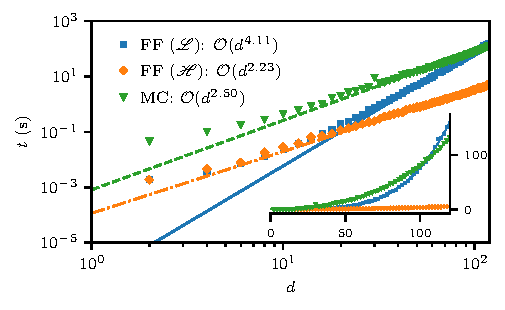
\includegraphics{img/pdf/benchmark_MC_vs_FF_linear-inset.pdf}
    \caption{
        Performance of the formalism using \cref{eq:ff:control_matrix:pulse:freq:ff:calculation} compared to a Monte Carlo method for a single gate as a function of problem dimension $d$.
        Parameters are: $n_{\Delta t} = \num{1}, n_\alpha = 3, n_\mr{MC} = 100, f_\mr{UV} = \flatfrac{10^2}{\Delta t}, n_\omega = \num{500}$ where $n_\alpha$ is the number of noise operators considered, $n_\mr{MC}$ the number of Monte Carlo trajectories over which is averaged, and $n_\omega$ the number of frequency samples.
        The calculation using filter functions clearly outperforms MC for small system sizes.
        For dimensions larger than $d\approx\num{100}$ (roughly equivalent to 7 qubits) Monte Carlo (blue squares) performs better than the \gls{ff} calculation with transfer matrices (green triangles) for this set of parameters and processor due to the better scaling behavior.
        Using conjugation by unitaries (orange diamonds) significantly outperforms \gls{mc} also for large dimensions.
        While the fits to $t = a d^b$ (lines) underestimate the leading order exponent due to the data not being in the asymptotic regime, they support the expected relationship of complexity between the approaches.
        The inset shows the same data on a linear scale, highlighting the different scaling behaviors for large $d$.
    }
    \label{fig:ff:performance:MC_vs_FF}
\end{figure}

Quantifying the performance gain from using the control matrices' concatenation property to calculate fidelities of gate sequences is more difficult since it strongly depends on the number of gates occurring multiple times in the sequence (enabling reuse of precomputed control matrices) as well as the complexity of the individual gates.
The evaluation using the concatenation rule \cref{eq:ff:control_matrix:sequence:freq} performs asymptotically worse than the evaluation for a complete pulse according to \cref{eq:ff:control_matrix:pulse:freq:ff:calculation} because of higher powers of $d$ dominating the calculation in the former case.
Performing the $G$ matrix multiplications $\ctrlmat\gth{g}(\omega)\liouvQ\gth{g-1}$ from \cref{eq:ff:control_matrix:sequence:freq} is of order $\sim G n_\omega n_\alpha d^4$, with $G$ the number of pulses in the sequence.
Furthermore, calculating the transfer matrix of the total propagators $Q_{g-1}$ involves multiplication of $d\times d$ matrices for all $d^4$ combinations of basis elements amounting to $\sim G d^{b+4}$.
In case the Liouville representation of the individual pulses' total propagators $P_g$, $\liouvP\gth{g}$, have been precomputed, the latter computation can be made more efficient since one can just propagate the transfer matrices $\liouvP\gth{g}$ to obtain the cumulative transfer matrices for the sequence, $\liouvQ\gth{g}=\prod_{g'=g}^0\liouvQ\gth{g'}$, at cost $\sim G d^{2b}$.
The restriction to small dimensions does not apply for conjugation by unitaries as in this case the matrix multiplications involve $d\times d$ matrices and we do not have to compute the Liouville representation.
We thus obtain a more favorable asymptotic scaling of $\sim G n_\omega n_\alpha d^b$.

Utilizing the concatenation property in the Liouville representation thus corresponds to effectively reducing the number of times the calculations scaling with $\sim n_\omega n_\alpha d^4$ have to be carried out but incurs additional calculations scaling with $\sim d^{2b}$.
Accordingly, it provides a performance benefit if a sequence consists of either very complex pulses, in which case single repetitions already make the calculation much more efficient, or of few pulses that occur many times.
In the extremal case of $G$ repetitions of a single gate the benefit of employing the concatenation property is most pronounced and can be improved even further utilizing the simplifications laid out in \cref{sec:ff:performance:periodic_hamiltonians}.
Since matrix inversion has the same complexity as matrix multiplication and taking a matrix to the $G$ power requires $\order{\log G}$ matrix multiplications, \cref{eq:ff:control_matrix:sequence:periodic:simplified} should scale with $\sim n_\omega (n_\alpha d^4 + d^{2b} + d^{2b}\log{G})$ (the first two terms are due to the final matrix multiplications and are independent of $G$).
It hence allows for a vast speedup over \cref{eq:ff:control_matrix:sequence:freq} in that the asymptotic behavior as a function of the number of gates changes from $\sim G$ to $\sim\log G$.
An example of this is presented in \cref{sec:ff:examples:rabi_driving} for the context of Rabi driving.
Note that this closed form is a unique feature of the transfer matrix representation and not applicable to conjugation by unitaries.

% ==================================================
%           SOFTWARE SECTION
% ==================================================
\chapter{Software implementation}\label{ch:ff:software}
In this section we give an overview over the \filterfunctions software package implementing the main features of the formalism derived above.
This includes the calculation of the decay amplitudes \decayamps and fidelities as well as the calculation of the control matrices for single gates and both generic and periodic sequences of gates.
Moreover, control matrices may be efficiently extended to and merged on larger Hilbert spaces.
Calculations using unitary conjugation instead of transfer matrices are implemented but at this point not available in the high-level API.

Our software is written in Python and available on GitHub~\cite{Hangleiter_ff} under the GPLv3 license.
We also provide a current snapshot in the Supplementary Material~\cite{prrSupp}.
It features a broad coverage through unit tests and extensive API documentation as well as didactic examples (see \cref{ch:ff:examples}).
The package relies on the \numpy~\cite{Harris2020} and \scipy~\cite{Virtanen2020} libraries for vectorized array operations.
Data visualization is handled by \matplotlib~\cite{Hunter2007}.
For tensor multiplications with optimized contraction order we use \opteinsum~\cite{Smith2018} for which \sparse~\cite{Pydata2019}, a library aiming to extend the \scipy sparse module to multi-dimensional arrays, serves as a backend in the calculation of the trace tensor from \cref{eq:ff:trace_tensor}.
Lastly, the package is written to interface with \qopt~\cite{Teske2021,Teske2022} and \qutip~\cite{Johansson2013}, frameworks for the simulation and optimization of open quantum systems, and mirrors the latter's data structure for Hamiltonians ensuring easy interoperability between the two.

\section{Package overview}\label{sec:ff:software:overview}
In the \filterfunctions package all operations are understood as sequences of pulses that are applied to a quantum system.
These pulses are represented by instances of the \pulsesequence class which holds information about the physical system (control and noise Hamiltonians) as well as the mathematical description (\eg the basis used for the Liouville representation).
As indicated above, the Hamiltonians $\Hc(t)$ and $\Hn(t)$ are given in a similar structure as in \qutip.
That is, a Hamiltonian is expressed as a sum of Hermitian operators with the time dependence encoded in piecewise constant coefficients so that
\begin{subequations}\label{eq:ff:hamiltonian:software}
\begin{gather}
    \Hc(t) = \sum_i a\gth{g}_i A_i = \mr{const.} \label{eq:ff:hamiltonian:software:control} \\
    \Hn(t) = \sum_\alpha s\gth{g}_\alpha B_\alpha = \mr{const.} \label{eq:ff:hamiltonian:software:noise}
\end{gather}
\end{subequations}
for $t\in (t_{g-1}, t_g], g\in\lbrace 1,\dotsc,G\rbrace$ and where the $a\gth{g}_i$ are the amplitudes of the $i$ control field.
Note that the noise variables $b_\alpha(t)$ are missing from \cref{eq:ff:hamiltonian:software:noise} because they are captured by the spectral density $S(\omega)$.
In the software, \cref{eq:ff:hamiltonian:software:control,eq:ff:hamiltonian:software:noise} are represented as lists whose $i$ element corresponds to a sublist of two elements: the $i$th operator and the $i$th coefficients $[a_i\gth{0},\dotsc,a_i\gth{G}]$.

The \pulsesequence class provides methods to calculate and cache the filter function according to \cref{eq:ff:control_matrix:pulse:freq}.
Alternatively, filter functions may also be cached manually to permit using the package with analytical solutions for the control matrix.
Concatenation of pulses is implemented by the functions \verb|concatenate()| and \verb|concatenate_periodic()| which will attempt to use the cached attributes of the \pulsesequence instances representing the pulses to efficiently calculate the filter function of the composite pulse following \cref{eq:ff:control_matrix:sequence:freq} and \cref{eq:ff:control_matrix:sequence:periodic:simplified}, respectively.

Operator bases fulfilling \cref{eq:ff:basis} are implemented by the \verb|Basis| class.
There are two predefined types of bases:
\begin{enumerate}
    \item Pauli bases for $n = 2^d$ qubits from \cref{eq:ff:basis:pauli} and
    \item generalized Gell-Mann (GGM) bases of arbitrary dimension $d$ from \cref{eq:ff:basis:ggm}.
\end{enumerate}
The Pauli basis is both unitary and separable while the GGM basis is sparse for large dimensions but neither unitary nor separable.
As mentioned in \cref{sec:ff:performance:extending_hilbert_spaces} (see also \cref{sec:ff:examples:qft}), using a separable basis can provide significant performance benefits for calculating the filter functions of algorithms.
On the other hand, a sparse basis makes the calculation of the trace tensor $T_{ijkl}$ and therefore also of the error transfer matrix \liouvUe much faster (\cf \cref{sec:ff:performance:basis}).
Additionally, the user can define custom bases using the class constructor.

The error transfer matrix \liouvUe can be calculated for a given pulse and noise spectrum using the \verb|error_transfer_matrix()| function \sidenote{Note that while the calculation of the frequency shifts \freqshifts is implemented, it should at time of publication be understood as preliminary and not thoroughly tested}.
Various other quantities can be computed from \liouvUe as outlined in \cref{sec:ff:theory:derived_quantities}.
Furthermore, the package includes a plotting module that offers several functions, \eg for the visualization of filter functions or the evolution of the Bloch vector using \qutip.

\section{Workflow}\label{sec:ff:software:workflow}
We now give a short introduction into the workflow of the \filterfunctions package by showing how to calculate the dephasing filter function of a simple Hahn spin echo sequence~\cite{Hahn1950} as an example.
The sequence consists of a single $\pi$-pulse of finite duration around the $x$-axis of the Bloch sphere in between two periods of free evolution.
We can hence divide the control fields into three constant segments and write the control Hamiltonian as
\begin{equation}
    \Hc\gth{\mr{SE}}(t) = \frac{\px}{2}\times\begin{cases}
        \flatfrac{\pi}{t_\pi},  &\mr{if\;} \tau\leq t < \tau + t_\pi \\
        0,                      &\mr{otherwise} \\
    \end{cases}
\end{equation}
with $\tau$ the duration of the free evolution period and $t_\pi$ that of the $\pi$ pulse.
For the noise Hamiltonian we only need to define the deterministic time dependence $s_\alpha(t)$ and operators $B_\alpha$ since the noise strength is captured by the spectrum $S(\omega)$.
Thus we have $s_z(t) =  1$ and $B_z = \flatfrac{\pz}{2}$ for pure dephasing noise that couples linearly to the system.

In the software, we first define a \pulsesequence object representing the spin echo (SE) sequence.
As was already mentioned, the control and noise Hamiltonians are given as a list containing lists for every control or noise operator that is considered.
These sublists consist of the respective operator as a \numpy array or \qutip \qobj and the amplitudes ($a_i\gth{g}$ or $s_\alpha\gth{g}$) in an iterable data structure such as a list.
We can hence instantiate the \pulsesequence with the following code:
\begin{lstlisting}{language=Python}
import filter_functions as ff
import qutip as qt
from math import pi
tau, t_pi = (1, 1e-3)
# Control Hamiltonian for pi rotation in 2nd time step
H_c = [[qt.sigmax()/2, [0, pi/t_pi, 0]]]
# Pure dephasing noise Hamiltonian with linear coupling
H_n = [[qt.sigmaz()/2, [1, 1, 1]]]
# Durations of piecewise constant segments
dt = [tau, t_pi, tau]
ECHO = ff.PulseSequence(H_c, H_n, dt)
\end{lstlisting}
where a basis is automatically chosen since we did not specify it in the constructor in the last line.
Calculating the filter function of the pulse for a given frequency vector \verb|omega| can then be achieved by calling
\begin{lstlisting}{language=Python}
F = ECHO.get_filter_function(omega)
\end{lstlisting}
where \verb|F| is the dephasing filter function $F_{zz}(\omega)$ as we only defined a single noise operator.
Finally, we calculate the error transfer matrix \liouvUe for the noise spectral density $S_{zz}(\omega) = \omega^{-2}$,
\begin{lstlisting}{language=Python}
S = 1/omega**2
U = ff.error_transfer_matrix(ECHO, S, omega)
\end{lstlisting}
This code uses the control matrix previously cached when the filter function was first computed.
Therefore, only the integration in \cref{eq:ff:decay_amplitudes:freq} and the calculation of the trace tensor in \cref{eq:ff:trace_tensor} are carried out in the last line.

An alternative approach to calculate the spin echo filter function is to employ the concatenation property.
For this, we interpret the SE as a sequence consisting of three separate pulses.
Each of the pulses has a single time segment during which a constant control is applied and concatenating the separate \pulsesequence instances yields the \pulsesequence representing a spin echo.
This way analytic control matrices may be used to calculate the control matrix of the composite sequence.
Pulses can be concatenated by using either the \verb|concatenate()| function or the overloaded \verb|@| operator:
\begin{lstlisting}{language=Python}
# Define PulseSequence objects as shown above
FID = ff.PulseSequence(...)
NOT = ff.PulseSequence(...)
# Cache the analytic control matrices at frequency omega
FID.cache_control_matrix(omega, B_FID)
NOT.cache_control_matrix(omega, B_NOT)
# Concatenate the pulses
ECHO = FID @ NOT @ FID
\end{lstlisting}
Since we have cached the control matrices of the \texttt{FID} and \texttt{NOT} pulses, that of the \texttt{ECHO} object is also automatically calculated and stored.
Concatenating \pulsesequence objects is implemented as an arithmetic operator of the class to reflect the intrinsic composition property of the control matrices.

Further development of the software has focused on making it available in a gate optimization and simulation framework~\cite{Teske2021,Teske2022}.
Besides using it to compute decoherence effects and fidelities, analytic derivatives of the filter functions have been implemented to allow for optimizing pulse parameters in the presence of non-Markovian noise within the framework of quantum optimal control~\cite{Le2022}.

Additionally, building an interface with \qupulse~\cite{Humpohl,Humpohl2021}, a software toolkit for parametrizing and sequencing control pulses and relaying them to control hardware, would implement the capability to compute filter functions of pulses assembled in \qupulse, thereby allowing a user in the lab to easily inspect the noise susceptibility characteristics of the pulse they are currently applying to their device.

% ==================================================
%           EXAMPLES SECTION
% ==================================================
\chapter{Example applications}\label{ch:ff:examples}
We now present example applications of the software package and the formalism.
As stated before, we focus on the decay amplitudes \decayamps and its associated filter functions and assume that the unitary errors generated by the frequency shifts \freqshifts are either small (as is the case for gate fidelities) or calibrated out.
All of the examples shown below are part of the software documentation as either interactive \jupyter notebooks~\cite{Kluyver2016} or Python scripts.
In the following, we give angular frequencies and energies in units of inverse times (\eg \si{\per\second}) while ordinary frequencies are given in \si{\hertz} and we write $\ev*{\liouvUe(\tau)} = \liouvUe$ for legibility.

\section{Singlet-triplet two-qubit gates}\label{sec:ff:examples:optimized_gates}
In order to benchmark fidelity predictions of our implementation as well as demonstrate its application to nontrivial pulses, we compute the first-order infidelity of the two-qubit gates presented in~\citer{Cerfontaine2020b} and compare the results to the reference's Monte Carlo calculations.
There, a numerically optimized gate set consisting of $\lbrace\mr{X}_{\flatfrac{\pi}{2}}\otimes\mr{I},\mr{Y}_{\flatfrac{\pi}{2}}\otimes\mr{I},\mr{CNOT}\rbrace$ for exchange-coupled singlet-triplet spin qubits is introduced, taking into account different noise spectra and realistic control hardware.

For readers unfamiliar with the reference we briefly summarize the physical system and noise model entering the optimization.
The authors consider four electrons confined in a linear array of four quantum dots in a semiconductor heterostructure.
Each electron $i\in\lbrace 1,2,3,4\rbrace$ experiences a different static magnetic field $B_i$ so that there is a gradient $b_{ij} = B_i - B_j$ between two adjacent dots $i$ and $j$.
This gives rise to spin quantization along the magnetic field axis and defines the eigenstates $\lbrace\ketud,\ketdu\rbrace$ that span the computational subspace of a single qubit so that the accessible Hilbert space of the two-qubit system is spanned by $\lbrace\ketud,\ketdu\rbrace^{\otimes 2}$.
The magnitude of the exchange interaction $J_{ij}$ between two adjacent dots $i$ and $j$ is controlled via gate electrodes located on top of the heterostructure that can be pulsed on a nanosecond timescale with an arbitrary waveform generator (AWG).
Changing the gate voltages changes the detuning $\eps_{ij}$ of the electrochemical potential between dots and in turn leads to a change in exchange coupling according to the phenomenological model $J_{ij}(\epsilon_{ij})\propto\exp(\epsilon_{ij})$.

The pulses are defined by a set of discrete detuning voltages $\epsilon_{ij}$ passed to an AWG with a sample rate of \qty{1}{\giga S\per\second} and constant magnetic field gradients $b_{ij}$ are assumed.
To reflect the fact that the qubits experience a different pulse than what is programmed into the AWG due to cable dispersion and non-ideal control hardware, the detunings are convoluted with an experimental impulse response~\cite{Cerfontaine2020b}.
Finally, the signal is discretized as piecewise constant by slicing each segment into five steps, yielding a time increment of $\Delta t = \qty{0.2}{\nano\second}$.

To find optimal detuning pulses, a Levenberg-Marquardt algorithm iteratively minimizes the infidelity, leakage, and trace distance from the target unitary.
For the infidelity, contributions from quasistatic magnetic field noise as well as quasistatic and white charge noise are taken into account during each iteration.
Because treating colored (correlated) noise using Monte Carlo methods is computationally expensive (\cf \cref{sec:ff:performance:complexity}), the infidelity due to fast \oneoverf-like noise is only computed for the final gate and not used during the optimization.

Two-qubit interactions are mediated via the exchange $J_{23}$ that makes the states \ketuudd and \ketdduu accessible.
They constitute levels outside of the computational subspace that ideally should only be occupied during an entangling gate operation.
A non-vanishing population of these states after the operation has ended is therefore unwanted and considered leakage, the magnitude of which we could quantify following \cref{sec:ff:theory:derived_quantities:leakage}.
However, here we limit ourselves to determine the infidelity contribution from fast, \viz non-quasistatic, charge noise entering the system through $\epsilon_{ij}$.
That is, we consider noise sources $\alpha\in\lbrace\epsilon_{12},\epsilon_{23},\epsilon_{34}\rbrace$.
We take the non-linear dependence of the Hamiltonian on the detunings $\epsilon_{ij}$ into account by setting $s_{\epsilon_{ij}}(t) = \pdv*{J_{ij}(\epsilon_{ij}(t))}{\epsilon_{ij}(t)}\propto J_{ij}(\epsilon_{ij}(t))$.

\Cref{fig:ff:CNOT} shows the filtered (convoluted) exchange interaction $J_{ij}$ between each pair of dots during the pulse sequence in panel (a) and filter functions plotted as function of frequency in panel (b) for the three different detunings.
For a detailed description on how the filter functions were computed in the presence of additional leakage levels refer to \cref{sec:app:ff:singlet-triplet}.
As one would expect from the fact that the intermediate (inter-qubit) exchange interaction $J_{23}$ (orange dash-dotted lines) is only turned on for short times to entangle the qubits, the filter function for $\eps_{23}$ is smaller by roughly an order of magnitude than the intra-qubit exchange filter functions.
Notably, the filter functions for $\eps_{12}$ and $\eps_{34}$ show clear characteristics of DCGs, that is they drop to zero as $\omega\rightarrow 0$, and decouple from quasistatic noise with an error suppression $\propto\omega^2$.
This is not unexpected as the optimization minimizes quasistatic noise contributions to the infidelity.
In addition, one can also observe small oscillations with period $\qty{5}{\per\nano\second}$ in frequency space that arise as a numerical artifact of the piecewise constant discretization of the control parameters as investigations have shown.
If high-frequency spectral components are expected to play a significant role, one needs to be aware of these effects and adjust the simulation parameters appropriately.

The inset of \cref{fig:ff:CNOT}(b) shows the same filter functions for the DC tail on a linear scale.
Most notably, $F_{\epsilon_{12}}$ and $F_{\epsilon_{34}}$ have maxima around $\omega = \flatfrac{2\pi}{\tau}$, \ie exactly the frequency matching the pulse duration, and around $\omega = \flatfrac{50}{\tau} = \qty{1}{\per\nano\second}$ with $\tau_\mr{CNOT} = \qty{50}{\nano\second}$.
The former is the typical window in which a pulse is most susceptible to noise whereas the latter matches the absolute value of the magnetic field gradients, $b_{12} = -b_{34} = \qty{1}{\per\nano\second}$, indicating that the peak corresponds to the qubit dynamics generated by the magnetic field gradients.
Panels (c)--(e) show the cumulant functions $\cumulantfun_{\eps_{ij}}(\tau)$ of the detuning error channels $\eps_{ij}$ on the computational subspace.
$\cumulantfun_{\eps_{12}}$ displays clear characteristics of a Pauli channel with only elements on the diagonal and secondary diagonals deviating from zero significantly whereas $\cumulantfun_{\eps_{34}}$ (the target qubit) possesses a more complicated structure.

\begin{figure*}[tbp]
    \centering
    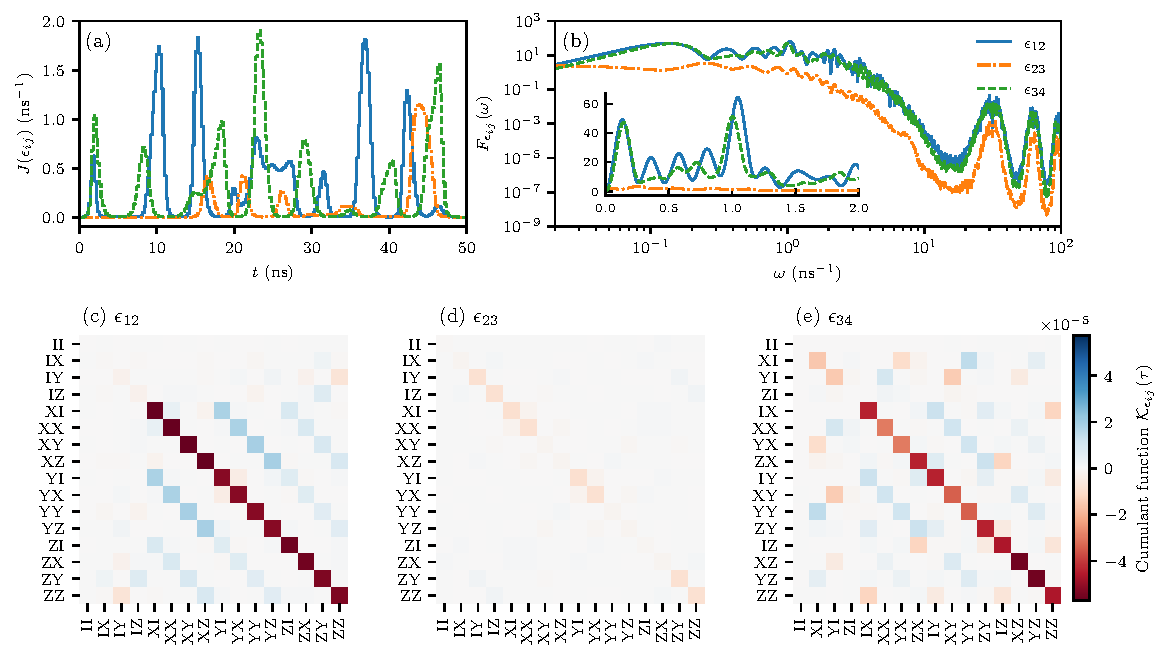
\includegraphics[width=\textwidth]{img/pdf/all_in_one_alpha-0-7_linear_complete_CNOT.pdf}
    \caption{
        (a) Exchange interaction $J(\epsilon_{ij})$ for the CNOT gate presented in~\citer{Cerfontaine2020b} as function of time.
        (b) Filter functions $F_{\epsilon_{ij}}$ for noise in the detunings evaluated on the computational subspace.
        The filter functions are modulated by oscillations at high frequencies due to numerical artifacts of the finite step size for the time evolution.
        The inset shows the filter functions in the DC regime on a linear scale with distinct peaks around $\omega = \flatfrac{2\pi}{\tau}$ and $\omega = \flatfrac{50}{\tau}$ ($\tau = \qty{50}{\nano\second}$).
        (c)--(e) Computational subspace block of the first order approximation of the error transfer matrix, given by the cumulant function $\cumulantfun_{\alpha\alpha}$ excluding second order contributions, for the CNOT gate and the three detunings $\alpha\in\lbrace\epsilon_{12},\epsilon_{23},\epsilon_{34}\rbrace$.
        Note that in panel (e) the order of the rows and columns was permuted for better comparability.
    }
    \label{fig:ff:CNOT}
\end{figure*}

We now compute the infidelity contribution originating from fast charge noise using \cref{eq:ff:fidelity:avg} but tracing only over the computational subspace to compare to the Monte Carlo calculations of~\citer{Cerfontaine2020b} (see \cref{sec:app:ff:singlet-triplet} for further details).
Like the reference, we use a noise spectrum $S_{\epsilon,a}(f)\propto \flatfrac{1}{f^a}$ with $S_{\epsilon,a}(\qty{1}{\MHz}) = \qty{4e-20}{\volt\squared\per\Hz}$ and consider white noise ($a = 0$) and correlated noise with $a = 0.7$~\cite{Dial2013} with infrared and ultraviolet cutoffs $\flatfrac{1}{\tau}$ and $\qty{100}{\per\nano\second}$, respectively.
\Cref{tab:ff:infidelities} compares the results in this work with the reference.
The values computed here are consistent with the more elaborate Monte Carlo calculations within a few percent.
Notably, the deviation is smaller for the smaller noise levels with $a = \num{0.7}$, in line with the fact that we have only computed the contributions from the decay amplitudes \decayamps and thus the leading order perturbation.
If we had additionally evaluated the frequency shifts \freqshifts we could have obtained the exact fidelity in the case of Gaussian noise.

\begin{table}
    \centering
    \renewcommand\arraystretch{1.25}
    \newlength{\colwidth}
    \setlength{\colwidth}{1.65 cm}
    %\renewcommand\tabcolsep{0pt}
    \begin{tabular*}{\columnwidth}{l *{4}{S[table-number-alignment=center,table-text-alignment=left,table-format=+1.1e+3,round-mode=figures,round-precision=2,table-column-width=\colwidth]}}
                                                    & \multicolumn{2}{c}{This work}                     & \multicolumn{2}{c}{\citer{Cerfontaine2020b}}   \\
    \toprule
        $a$                                         & 0             & \sisetup{round-precision=1} 0.7   & 0             & \sisetup{round-precision=1} 0.7   \\
    %\colrule
    \midrule
        $\mr{X}_{\flatfrac{\pi}{2}}\otimes\mr{I}$   & 1.679e-03     & 5.837e-05                         & 1.892e-03     & 5.737e-05                         \\
        $\mr{Y}_{\flatfrac{\pi}{2}}\otimes\mr{I}$   & 1.595e-03     & 5.690e-05                         & 1.689e-03     & 5.622e-05                         \\
        CNOT                                        & 1.498e-03     & 6.399e-05                         & 1.560e-03     & 6.313e-05                         \\
    %\botrule
    \bottomrule
    \end{tabular*}
    \caption{
        Fast charge noise infidelity contributions to the total average gate fidelity of the two-qubit gate set from~\citer{Cerfontaine2020b} without capacitive coupling for GaAs \sts qubits compared to the original results.
        The fidelities are consistent with results from the reference within the uncertainty bounds of \qty{3}{\percent} of the Monte Carlo calculation.
        The infidelities presented here are all average gate infidelities (cf.
        \cref{eq:ff:fidelity:avg},~\citerr{Horodecki1999}{Nielsen2002}).
    }
    \label{tab:ff:infidelities}
\end{table}

\section{Rabi driving}\label{sec:ff:examples:rabi_driving}
A widely used method for qubit control is Rabi driving~\cite{Wallraff2004,Barends2014,Soare2014,Veldhorst2014}.
If we restrict ourselves to the resonant case for simplicity, the control Hamiltonian takes on the general form $\Hc = \flatfrac{\omega_0\pz}{2} + A\sin(\omega_0 t + \phi)\px$.
Here, $\omega_0$ is the resonance frequency, $A$ the drive amplitude corresponding to the Rabi frequency in the weak driving limit $\flatfrac{A}{\omega_\mr{0}}\ll 1$, $\Omega_\mr{R}\approx A$, and $\phi$ an adjustable phase giving control over the rotation axis in the $xy$-plane of the Bloch sphere.
This Hamiltonian and associated decoherence mechanisms are well-studied in the weak driving regime, where the rotating wave approximation (RWA) can be applied to remove fast-oscillating terms in the rotating frame~\cite{Jaynes1963,Gerry2008}.
There is a comprehensive understanding of how spectral densities transform to this frame and which frequencies are most relevant to loss of coherence~\cite{Yan2013}.

By contrast, the description of a system in the strong driving regime, where $\flatfrac{A}{\omega_0}\sim 1$, is more complicated since the RWA cannot be applied without making large errors.
Yet, an improved understanding is desirable because strong driving allows for much shorter gate times and thus shifts the window of relevant noise frequencies towards higher energies where the total noise power is typically lower, \eg for \oneoverf noise.
Conversely, faster control also requires more accurate timing to prevent rotation errors.
It is therefore of interest to have available tools that can provide a comprehensive picture for Rabi pulses over a wide range of driving amplitudes.
By making use of the concatenation property of the filter functions, our formalism can do just that.

The problem that arises when trying to numerically investigate Rabi pulses in the weak driving regime in the lab frame is that typical control operations have a duration $\tau\gg T$ with $T = \flatfrac{2\pi}{\omega_0}$.
Since the sampling time step $\Delta t$ should additionally be chosen much smaller than a single drive period in order to sample the time evolution accurately ($\Delta t\ll T$), brute-force simulations are costly.

For $\flatfrac{T}{\Delta t} = 100$ samples per period and assuming Rabi and drive frequencies in typical regimes for SiGe and MOS quantum dots~\cite{Zajac2018,Pla2012} or trapped ions~\cite{Soare2014}, $\Omega_\mr{R} = \qty{1}{\per\micro\second}$ and $\omega_0 = \qty{20}{\per\nano\second}$, a Monte Carlo simulation of a $\pi$-rotation with approximately \qty{3}{\percent} relative error would require $10^9$ samples in total.
Using the filter function formalism, we can drastically reduce the simulation time even beyond the improvement gained from concatenating precomputed filter functions of individual drive periods using \cref{eq:ff:control_matrix:sequence:freq}.
This can be achieved with \cref{eq:ff:control_matrix:sequence:periodic:simplified}, which simplifies the calculation of the control matrix for periodic Hamiltonians.

To benchmark our implementation, we use the parameters from above and calculate the control matrix of a NOT gate generated by a Rabi Hamiltonian with three different methods on an \fastprocessor.
First, we use \cref{eq:ff:control_matrix:sequence:freq} in a brute force approach.
Second, we utilize the concatenation property following \cref{eq:ff:control_matrix:pulse:freq:ff:calculation}.
Third, we employ the simplified expression given by \cref{eq:ff:control_matrix:sequence:periodic:simplified}.
The brute force approach takes \qty{250}{\second} of wall time whereas calculating the filter function using the standard concatenation is faster by two orders of magnitude, taking \qty{1.5}{\second} to run.
Lastly, the calculation utilizing the optimized method is faster again by two orders of magnitude and is completed in \qty{0.056}{\second}.

%\begin{table}[tbp]
%    \renewcommand\arraystretch{1.25}
%    %\setlength{\colwidth}{0.85 cm}
%    %\renewcommand\tabcolsep{0pt}
%    %\begin{tabular*}{\columnwidth}{l @{\extracolsep{\fill}} *{3}{S[table-number-alignment=center,table-text-alignment=center,round-mode=figures,round-precision=2]}}
%    \begin{tabular*}{\columnwidth}{@{\extracolsep{\fill}} *{4}{l}}
%    \toprule
%    Calculation method      & \cref{eq:ff:control_matrix:pulse:freq:ff:calculation}   & \cref{eq:ff:control_matrix:sequence:freq}    & \cref{eq:ff:control_matrix:sequence:periodic:simplified} \\
%    \colrule
%    %\midrule
%    Wall time (\si{\second})& 370                                               & 1.3                                       & 0.079         \\
%    %Wall time (\si{\second})& 367.4646                                          & 1.2895                                    & 0.0793       \\
%    %\bottomrule
%    \botrule
%    \end{tabular*}
%    \caption{Approximate wall times on an \fastprocessor for different ways of computing the control matrix of a Rabi-driven NOT gate with $10^6$ time steps and 500 frequency points highlighting the drastic performance improvement of using the optimized expressions.}
%    \label{tab:ff:rabi_driving:benchmark}
%\end{table}

As an example application, we calculate the filter functions for continuous Rabi driving in the weak and strong driving regimes.
For weak driving, we use the parameters from the benchmark above for a pulse of duration $\tau_\mr{weak}\approx\qty{20}{\micro\second}$ that corresponds to \num{20} identity rotations in total.
For the strong driving regime, we use the approximate analytical solution for a flux qubit biased at its symmetry point from~\citer{Deng2015} with $A = \flatfrac{\omega_0}{4}$ to drive the qubit for $\tau_\mr{strong}\approx\qty{4}{\nano\second}$ so that we achieve the same amount of identity rotations as in the weak driving case.
In the reference, strong driving in this regime is shown to give rise to non-negligible counterrotating terms that modulate the Rabi oscillations and which are well-described by Floquet theory applied to the Rabi driving Hamiltonian.
While for the regime studied here only two additional modes appear, the results extend to the regime where $A > \omega_0$ and up to eight different frequency components were observed.

\Cref{fig:ff:filter_function:rabi:weak_vs_strong} shows the filter functions $F_{xx}$ and $F_{zz}$ for the \px and \pz noise operators in the weak (a) and the strong (b) driving regime.
Both display sharp peaks at their Rabi frequencies and the resonance frequency for $F_{zz}$ and $F_{xx}$, respectively.
We expect these features as they correspond to perturbations of the qubit Hamiltonian that are resonant with the qubit dynamics about an axis orthogonal to them.
For weak driving, $F_{xx}$ is constant up to the resonance frequency where it peaks sharply and then aligns with $F_{zz}$.
The latter has a peak at the Rabi frequency before rolling off with $\omega^{-2}$ and a DC level that is almost ten orders of magnitude larger than that of the transverse filter function.
This behavior is consistent with the results by~\citeauthor{Yan2013}, who show that the noise sources dominating decoherence during driven evolution are $S_{xx}(\omega_0)$ and $S_{zz}(\Omega_\mr{R})$.
Note that the piecewise constant control approximation causes the weak driving filter functions to level off towards low frequencies after an initial roll-off (here at $\omega\sim\qty{1}{\per\milli\second}$).
By decreasing the discretization time step $\Delta t$, one can shift the frequency at which this effect occurs to lower frequencies and thus attribute the feature to a numerical artefact of the approximation.
However, the decoupling properties depend quite sensitively on the pulse duration.

In case of strong driving, the two filter functions are closer in amplitude for lower frequencies.
In addition, $F_{xx}$ also peaks at $\omega = \omega_0\pm\Omega_\mr{R}$.
These peaks also show up at higher frequencies in the dephasing filter function $F_{zz}$, reflecting frequency mixing in the strong coupling regime.
While both filter functions show characteristics of a DCG in the weak driving regime, that is they drop to zero as $\omega\rightarrow 0$, this is not the case in the strong driving regime.
Instead, there they approach a constant level for small frequencies.
On top of rotation errors from timing inaccuracies, we may thus expect naive strong driving gates to be more susceptible to quasistatic noise than weak driving gates.
By shaping the pulse envelope of the strong driving gate the decoupling properties could be recovered.

\begin{figure}[tbp]
    \centering
    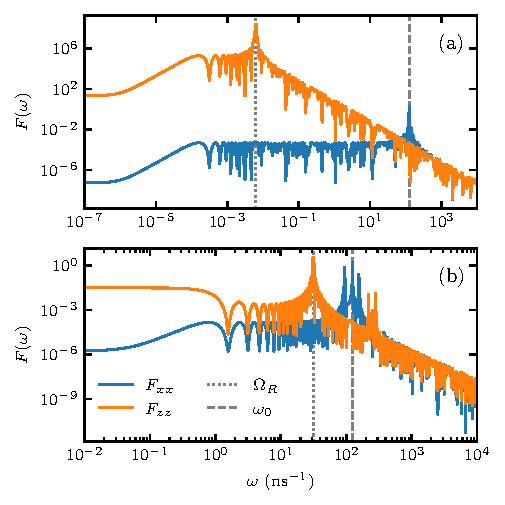
\includegraphics{img/pdf/rabi_driving_weak_vs_strong.pdf}
    \caption{
        Filter functions for weak (a) and strong (b) Rabi driving (\num{20} identity gates in total).
        Grey dashed (dotted) lines indicate the respective drive (Rabi) frequencies $\omega_0$ ($\Omega_\mr{R}$).
        (a) Weak driving with $\flatfrac{A}{\omega_\mr{0}}\ll 1$.
        The filter function $F_{xx}$ for noise operator \px is approximately constant up to the resonance frequency where it peaks sharply and then aligns with the filter function $F_{zz}$ for \pz.
        $F_{zz}$ peaks at the Rabi frequency before rolling off with $\omega^{-2}$ and a DC level that is almost ten orders of magnitude larger than the DC level of the transverse filter function $F_{xx}$.
        (b) Strong driving with $\flatfrac{A}{\omega_\mr{0}}\sim 1$.
        Again $F_{zz}$ peaks at $\Omega_\mr{R}$ whereas $F_{xx}$ has three distinct peaks at $\omega_\mr{0}$ and $\omega_\mr{0}\pm\Omega_\mr{R}$.
        These features also appear at slightly higher frequencies in $F_{zz}$ due to the strong coupling.
    }
    \label{fig:ff:filter_function:rabi:weak_vs_strong}
\end{figure}

\section{Randomized Benchmarking}\label{sec:ff:examples:randomized_benchmarking}
\Gls{srb} and related methods, for example \gls{irb}, are popular tools to assess the quality of a qubit system and the operations used to control it~\cite{Knill2008,Magesan2011,Magesan2012a}.
The basic protocol consists of constructing $K$ random sequences of varying length $m$ of gates drawn from the Clifford group
\sidenote{The Clifford group is a subgroup of the special unitary group with the advantage that compositions are easy to compute and that averaging over all unitaries can under reasonable assumptions be replaced by averaging over all Cliffords.
This makes the Clifford gates a convenient choice for benchmarking.
For a nice, short introduction as well as further references, see~\cite{Ozols2008}},
and appending a final inversion gate so that the identity operation should be performed in total.
Each of these pulse sequences is applied to an initial state $\kpsi$ in order to measure the survival probability $p(\kpsi)$ after the sequence.
In reality, the applied operations are subject to noise and experimental imprecisions.
This renders them imperfect and results in a survival probability smaller than one.
Assuming gate-independent errors, the average gate fidelity $\avgfid$ is then obtained by fitting the measured survival probabilities for each sequence length to the zeroth-order exponential model~\cite{Magesan2011}
\begin{equation}\label{eq:ff:SRB}
    p(\kpsi) = A \left(1 - \frac{dr}{d-1}\right)^m + B,
\end{equation}
where $r = 1 - \avgfid$ is the average error per single gate to be extracted from the fit, $A$ and $B$ are parameters capturing state preparation and measurement (SPAM) errors, and $d$ is the dimensionality of the system.

One of the main assumptions of the \gls{srb} protocol is that temporal correlations of the noise are small on timescales longer than the average gate time~\cite{Magesan2011}.
If this requirement is not satisfied, \eg if \oneoverf noise plays a dominant role, the decay of the sequence fidelity can have non-exponential components~\cite{Epstein2014,Fogarty2015,Feng2016} and a single exponential fit will not produce the true average gate fidelity~\cite{Mavadia2018,Edmunds2020}.
The filter function formalism suggests itself to numerically probe \gls{rb} experiments in such systems for two reasons.
First, it enables the study of gate performance subject to noise with correlation times longer than individual gate times.
This regime, where a simple description in terms of individual, isolated quantum operations fails, is accessible in the filter function formalism because universal classical noise can be included by the power spectral density $S(\omega)$.
Second, the simulation of a \gls{rb} experiment can be performed efficiently by using the concatenation property.
Because \gls{rb} sequences are compiled from a limited set of gates whose filter functions may be precomputed, one only needs to concatenate $m$ filter functions for a single sequence of length $m$ to gain access to the survival probability.

Since for sufficiently long \gls{rb} sequences $r\in\order{1}$, and we would need to include the frequency shifts \freqshifts in a full simulation following \cref{eq:ff:cumulant_expansion} because the low-noise approximation \cref{eq:ff:error_transfer_matrix:approx} does not hold in this regime.
Unfortunately, the concatenation property does not hold for \freqshifts.
Therefore, we focus on the high-fidelity regime where the exponential decay of the sequence fidelity may be approximated to linear order and only the decay amplitudes \decayamps need to be considered.

In order to evaluate the survival probability of a \gls{rb} experiment using filter functions, we employ the state fidelity from \cref{sec:ff:theory:derived_quantities:state_fidelity-measurements} and focus on the single-qubit case with $d = 2$ and the (normalized) Pauli basis from \cref{eq:ff:basis:pauli}.
Because the ideal action of a \gls{rb} sequence is the identity we have $\liouvQ = \eye$.
Assuming we prepare and measure in the computational basis, $\kpsi\in\lbrace\ket{0}, \ket{1}\rbrace$ so that $\sqrt{2}\dket{\rho} = \dket{\sigma_0}\pm\dket{\sigma_3}$, we simplify \cref{eq:ff:fidelity:state} to
\begin{equation}\label{eq:ff:fidelity:state:RB}
    \begin{split}
        \fid(\kpsi, \liouvU_\mr{RB}(\op{\psi})) &= \frac{1}{2}\bigl(\liouvUe_{00} +
                                                                \liouvUe_{33}\pm
                                                                \liouvUe_{03}\pm
                                                                \liouvUe_{30}\bigr) \\
                                                &= \frac{1 + \liouvUe_{33}}{2} \approx 1 - \frac{1}{2}\sum_{k\neq 3}\decayamps_{kk}.
    \end{split}
\end{equation}
For the second equality we used that \liouvUe is trace-preserving and unital (\cf \cref{sec:ff:theory:transfer_matrix:derivation}) while in the last step we approximated the expression using \cref{eq:ff:error_transfer_matrix:approx,eq:ff:cumulant:truncated:liouville:pauli}.
For our simulation, we neglect SPAM errors so that $A =  B =  0.5$, choose $\kpsi = \ket{0}$, and approximate \cref{eq:ff:SRB} as
\begin{equation}\label{eq:ff:fidelity:state:RB:fit}
    p(\ket{0}) = \fid(\ket{0}, \liouvU_\mr{RB}(\op{0}))\approx 1 - rm
\end{equation}
for small gate errors $r\ll 1$ since this is the regime which we can efficiently simulate using the concatenation property.

We simulate single-qubit \gls{srb} experiments using three different gate sets to generate the 24 elements of the Clifford group.
For the first gate set we implement the group by naive \enquote{single} rotations about the symmetry axes of the cube.
Each pulse corresponds to a single time segment during which one rotation is performed so that the $j$ element is given by $Q_j = \exp(-\i\phi_j\vec{n}_j\times\vec{\sigma})$.
We compile the other two gate sets from primitive $\flatfrac{\pi}{2}$ $x$- and $y$-rotations so that on average each Clifford gate consists of \num{3.75} primitive gates (see~\citer{Cerfontaine2020}).
For the specific implementation of the primitive $\flatfrac{\pi}{2}$-gates we compare \enquote{naive} rotations, \ie with a single time segment so that $Q_j = \exp(\flatfrac{-\i\pi\sigma_j}{4})$ for $j\in\lbrace x, y\rbrace$, and the \enquote{optimized} gates from~\citer{Cerfontaine2020b}.
Pulse durations are chosen such that the average duration of all 24 Clifford gates generated from a single gate set is equal for all three gate sets.
This is to ensure that the different implementations of the Clifford gates are sensitive to the same noise frequencies.

We investigate white noise and correlated noise with $S(\omega)\propto\omega^{-0.7}$ assuming the same noise spectrum on each Cartesian axis of the Bloch sphere and normalize the noise power for each gate set and noise type (white and correlated) so that the average Clifford infidelity $r$ is the same throughout.
We then randomly draw $K = \num{100}$ sequences for \num{11} different lengths $m\in[1, 101]$ and concatenate the $m$ Clifford gates using \cref{eq:ff:control_matrix:sequence:freq} to compute the control matrix of the entire sequence.
For the integral in \cref{eq:ff:decay_amplitudes:freq} we choose the ultraviolet cutoff frequency two orders of magnitude above the inverse duration of the shortest pulse, $f_\mr{UV} = \flatfrac{10^2}{\tau_\mr{min}}$.
Similarly, the infrared cutoff is chosen as $f_\mr{IR} = \flatfrac{10^{-2}}{m_\mr{max}\tau_\mr{max}}$ with $m_\mr{max} = 101$ and $\tau_\mr{max} = 7\tau_\mr{min}$ (since the longest gate is compiled from seven primitive gates with duration $\tau_\mr{min}$) to guarantee that all nontrivial structure of the filter functions is resolved at small frequencies
\sidenote{For a precise fidelity estimate, the infrared cutoff should be extended to $f=0$.
However, we are only interested in a qualitative picture and neglect this part of the spectrum here.
At frequencies much smaller than $\approx\flatfrac{1}{\tau}$ where $\tau$ is the duration of the entire control operation, the filter function is constant and we therefore do not disregard any interesting features by setting $f_\mr{IR} = \flatfrac{10^{-2}}{\tau} = \flatfrac{10^{-2}}{m_\mr{max}\tau_\mr{max}}$.}.
%adequately.
Finally, we fit \cref{eq:ff:fidelity:state:RB:fit} to the infidelities computed for the different noise spectra.

The results of the simulation are shown in \cref{fig:ff:randomized_benchmarking:noise_comparison} (a) and (b) for white and correlated noise, respectively.
For white noise, the survival probability agrees well with the \gls{srb} prediction for all gate types whereas for \oneoverf-like noise the \enquote{single} gates (green pluses) deviate considerably.
Hence, fitting the zeroth-order \gls{srb} model to such data will not reveal the true average gate fidelity although errors are of order unity.
We note that~\citerr{Epstein2014}{Ball2016} found similar results using different methods for \oneoverf and perfectly correlated DC noise, respectively.
The former observed \gls{srb} to estimate $r$ within \qty{25}{\percent} and the latter found the mean of the \gls{srb} fidelity distribution to deviate from the mode, thereby giving rise to incorrectly estimated fidelities.

\begin{figure}[tbp]
    \centering
    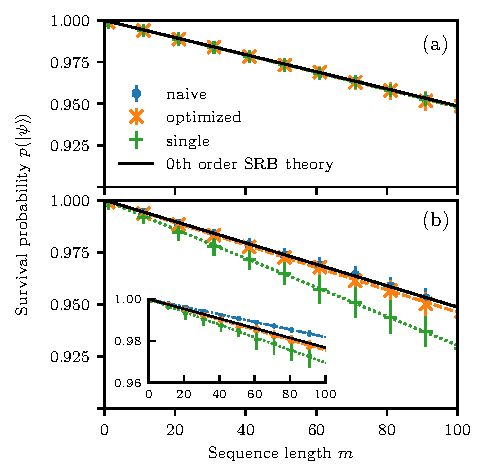
\includegraphics{img/pdf/RB_naive-optimized-single_gates_white_vs_correl_with_Z_noise_inset.pdf}
    \caption{
        Simulation of a \gls{srb} experiment using \num{100} random sequences per point for different gate and noise types (see the main text for an explanation of the gate type monikers).
        Dashed lines are fits of \cref{eq:ff:fidelity:state:RB:fit} to the data while the solid black lines correspond to a zeroth-order \gls{srb} model with $A=B=\num{0.5}$ and the true average gate infidelity per Clifford $r$.
        Errorbars show the standard deviation of the \gls{srb} sequence fidelities, illustrating that for the \enquote{single} gate set noise correlations can lead to amplified destructive and constructive interference of errors.
        The same noise spectrum is used for all three error channels (\px, \py, \pz) and the large plots show the sum of all contributions.
        (a) Uncorrelated white noise with the noise power adjusted for each gate type so that the average error per gate $r$ is constant over all gate types.
        No notable deviation is seen between different gate types.
        (b) Correlated \oneoverf-like noise with noise power adjusted to match the average Clifford fidelity in (a).
        The decay of the \enquote{single} gateset differs considerably from that of the other gate sets and the \gls{srb} decay expected for the given average gate fidelity, whereas \enquote{naive} and \enquote{optimized} gates match the zeroth order \gls{srb} model well, indicating that correlations in the noise affect the relation between \gls{srb} decay and average gate fidelity in a gateset-dependent way.
        Inset: contributions from \pz-noise show that the sequence fidelity can be better than expected for certain gate types and noise channels.
    }
    \label{fig:ff:randomized_benchmarking:noise_comparison}
\end{figure}

On top of affirming the findings by the references, our results demonstrate that the accuracy of the predictions made by \gls{srb} theory, \ie that the \gls{rb} decay rate directly corresponds to the average error rate of the gates, not only depends on the gate implementation but also on which error channels are assumed.
This can be seen from the inset of \cref{fig:ff:randomized_benchmarking:noise_comparison}(b), where only dephasing noise (\pz) contributions are shown.
For this noise channel and the \enquote{naive} gates, one finds a slower \gls{rb} decay than expected from the actual average gate fidelity, so that the latter would be overestimated by an \gls{rb} experiment, whereas the \enquote{single} gates show the opposite behavior.
Depending on the gate set and relevant error channels, non-Markovian noise may thus even lead to improved sequence fidelities due to errors interfering destructively.
This behavior is captured by the pulse correlation filter functions whose contributions to the sequence fidelity lead to the deviations from the \gls{srb} prediction.

Notably, the data for the \enquote{optimized} gates agree with the prediction for every noise channel individually which implies that correlations between pulses are suppressed.
This highlights the formalism's attractiveness for numerical gate optimization as the pulse correlation filter functions $F\gth{gg'}(\omega)$ may be exploited to suppress correlation errors.
To be more explicit, the correlation decay amplitudes $\decayamps\gth{gg'}$ from \cref{eq:ff:decay_amplitudes:pulse_correlation} can be used to construct cost functions for quantum optimal control algorithms like GRAPE~\cite{Khaneja2005,Schulte-Herbruggen2005} or CRAB~\cite{Caneva2011}.
By constructing linear combinations of $\decayamps\gth{gg'}$ with different pulse indices $g$ and $g'$, correlations between any number of pulses can be specifically targeted and suppressed using numerical pulse optimization.

\section{Quantum Fourier transform}\label{sec:ff:examples:qft}
To demonstrate the flexibility of our software implementation, we calculate filter functions for a four-qubit \acrfull{qft}~\cite{Coppersmith1994,Nielsen2011} circuit.
QFT plays an important role in many quantum algorithms such as Shor's algorithm~\cite{Shor1997} and quantum phase estimation~\cite{Nielsen2011}.
For the underlying gate set, we assume a standard Rabi driving model with IQ control and nearest neighbor exchange.
That is, we assume full control of the $x$- and $y$-axes of the individual qubits as well as the exchange interaction mediating coupling between two neighboring qubits.
This system allows for native access to the minimal gateset $\mathbb{G} = \lbrace\mr{X}_{i}(\flatfrac{\pi}{2}),\mr{Y}_{i}(\flatfrac{\pi}{2}),\mr{CR}_{ij}(\flatfrac{\pi}{2^3})\rbrace$ where $\mr{CR}_{ij}(\phi)$ denotes a controlled rotation by $\phi$ about $z$ with control qubit $i$ and target qubit $j$.
Controlled-$z$ rotations by angles $\flatfrac{\pi}{2^m}$ as required for the QFT can thus be obtained by concatenating $2^{3-m}$ minimal gates $\mr{CR}_{ij}(\flatfrac{\pi}{2^3})$.

Despite native access to all necessary gates, we employ \qutip's implementation~\cite{Johansson2013} of the GRAPE algorithm~\cite{Khaneja2005,Schulte-Herbruggen2005} to generate the gates in order to highlight our method's suitability for numerically optimized pulses.
For the optimization we choose a time step of $\Delta t = \qty{1}{\nano\second}$ and a total gate duration of $\tau = \qty{30}{\nano\second}$.
For completeness, see \cref{sec:app:ff:qft} for details on the optimized gates.
We then construct the remaining required gates by sequencing these elementary gates, \ie the Hadamard gate $\mr{H}_i = \mr{X}_{i}(\flatfrac{\pi}{2})\circ\mr{X}_{i}(\flatfrac{\pi}{2})\circ\mr{Y}_{i}(\flatfrac{\pi}{2})$, where $\mr{B}\circ\mr{A}$ denotes the composition of gates A and B such that gate A is executed before gate B.
To map the canonical circuit~\cite{Nielsen2011} onto our specific qubit layout with only nearest-neighbor coupling, we furthermore introduce SWAP operations to couple distant qubits.
These gates can be implemented by three CNOTs, $\mr{SWAP}_{ij} = \mr{CNOT}_{ij}\circ\mr{CNOT}_{ji}\circ\mr{CNOT}_{ij}$.
The CNOTs in turn are obtained by a Hadamard transform of the controlled phase gate, $\mr{CNOT}_{ij} = \mr{H}_j\circ\mr{CR}_{ij}(\pi)\circ\mr{H}_j$.
The complete quantum circuit is shown at the top of \cref{fig:ff:qft}; for the canonical circuit with all-to-all connectivity refer to~\citer{Nielsen2011}.
In total, there are \num{442} elementary pulses, \num{198} of which are required for the three SWAPs on the first two qubits, so that the entire algorithm would take $\sim\qty{13}{\micro\second}$ to run.
Note that the circuit could be compressed in time by parallelizing some operations but for simplicity we only execute gates sequentially and do not execute dedicated idling gates.

\begin{figure*}[tbp]
    %\resizebox{\columnwidth}{!}{}
    \centerline{\Qcircuit @C=1em @R=1.4em {
    \lstick{3}  & \qw       & \qw                           & \qw           & \qw                           & \qw           & \ctrl{1}                      & \qswap     & \qw      & \qw                           & \qw           & \qw                           & \qw           & \qw      & \qw                            & \qw           & \qw       & \qwa    & \rstick{0} \\
    \lstick{2}  & \qw       & \qw                           & \qw           & \ctrl{1}                      & \qswap        & \gate{R(\flatfrac{\pi}{2^3})} & \qswap\qwx & \qw      & \qw                           & \qw           & \ctrl{1}                      & \qswap        & \qw      & \qw                            & \qw           & \qw       & \qwa    & \rstick{1} \\
    \lstick{1}  & \qw       & \ctrl{1}                      & \qswap        & \gate{R(\flatfrac{\pi}{2^2})} & \qswap\qwx    & \qw                           & \qw        & \qw      & \ctrl{1}                      & \qswap        & \gate{R(\flatfrac{\pi}{2^2})} & \qswap\qwx    & \qw      & \ctrl{1}                       & \qswap        & \qw       & \qwa    & \rstick{2} \\
    \lstick{0}  & \gate{H}  & \gate{R(\flatfrac{\pi}{2^1})} & \qswap\qwx    & \qw                           & \qw           & \qw                           & \qw        & \gate{H} & \gate{R(\flatfrac{\pi}{2^1})} & \qswap\qwx    & \qw                           & \qw           & \gate{H} & \gate{R(\flatfrac{\pi}{2^1})}  & \qswap\qwx    & \gate{H}  & \qwa    & \rstick{3} 
    %\gategroup{3}{2}{4}{4}{1em}{--}
    %\gategroup{2}{5}{3}{6}{1em}{--}
    %\gategroup{2}{2}{4}{6}{1em}{--}
    %\gategroup{3}{9}{4}{11}{1em}{--}
    %\gategroup{2}{12}{3}{13}{1em}{--}
    %\gategroup{2}{9}{4}{13}{1em}{--}
    %\gategroup{3}{14}{4}{16}{1em}{--}
}}
    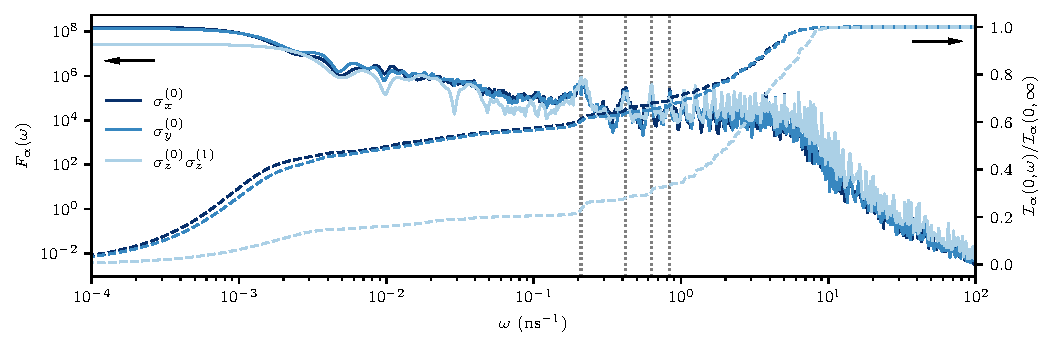
\includegraphics[width=\textwidth]{img/pdf/qft_filter_function_first_qubit_with_cumulative_fraction.pdf}
    \caption{
        Top: Circuit for a \gls{qft} on four qubits with nearest-neighbor coupling.
        Labels next to the wires indicate the qubit index, showing that the final SWAP operation has already been carried out.
        Bottom: Filter functions for noise operators on the first qubit ($i = 0$).
        Dotted grey lines indicate the positions of the $n$ harmonic, $\omega_n = \flatfrac{2\pi n}{\tau}$ with $\tau = \qty{30}{\nano\second}$ the duration of the gates in $\mathbb{G}$, for $n\in\lbrace 1, 2, 3, 4\rbrace$.
        The filter functions have a baseline of around $10^4$ in the range $\omega\in[10^{-1}, 10^{1}]$ \si{\per\nano\second} before they drop down to follow the usual $1/\omega^2$ behavior.
        The dashed lines show the error sensitivities $\mc{I}_\alpha(\omega_1,\omega_2)\coloneqq\int_{\omega_1}^{\omega_2}\dd{\omega} F_\alpha(\omega)$ in the frequency band $[0, \omega]$ as a fraction of the total sensitivity $\mc{I}_\alpha(0,\infty)$.
        These are closely related to the entanglement fidelity (\cf \cref{eq:ff:filter_function:fidelity,eq:ff:infidelity:ent:integral}) and suggest that high frequencies up to the knee at $\omega\approx\qty{10}{\per\nano\second}$ cannot be neglected if the cutoff frequency of the noise is sufficiently high or the spectrum does not drop off quickly enough (note the linear scale as opposed to the logarithmic scale for the filter functions).
    }
    \label{fig:ff:qft}
\end{figure*}

In order to leverage the extensibility of the filter function approach (see \cref{sec:ff:performance:extending_hilbert_spaces}), we use a Pauli basis for the pulses and proceed as follows:
\begin{enumerate}
    \item Instantiate the \pulsesequence objects for the elementary gates $\mathbb{G}$ for the first two qubits and cache the control matrices.
    \item Compile all required single- and two-qubit pulses by concatenating the \pulsesequences that implement $\mathbb{G}$.
    \item Extend the \pulsesequences to the full four-qubit Hilbert space.
    \item Recursively concatenate recurring gate sequences by concatenating four-qubit \pulsesequences, \eg $\mr{SWAP}_{10}\circ\mr{CR_{10}}(\flatfrac{\pi}{2^1})\circ\mr{H}_0$, in order to optimally use the performance benefit offered by \cref{eq:ff:control_matrix:sequence:freq}
    \item Concatenate the last \pulsesequences to get the complete QFT pulse.
\end{enumerate}
For our gate parameters and \num{400} frequency points, this procedure takes around \qty{5}{\second} on an \fastprocessor, whereas computing the filter functions naively using \cref{eq:ff:control_matrix:pulse:freq:ff:calculation} takes around \qty{4}{\minute}.
The resulting filter functions are shown in \cref{fig:ff:qft} for the noise operators affecting the first qubit; for an in-depth discussion and validation of the fidelities predicted, see the accompanying letter~\citer{Cerfontaine2021} and its supplementary information.
Evidently, the fidelity of the algorithm is most susceptible to DC noise; below roughly $\omega\lessapprox 10^{-3}\,\si{\per\nano\second}$ the filter functions level off at their maximum value.
In the \si{\giga\hertz} range there is a plateau with sharp peaks corresponding to the $n$ harmonics of the inverse pulse duration $\omega_n = \flatfrac{2\pi n}{\tau}$, where the leftmost belongs to $n=1$.
The dashed lines show the error sensitivities $\mc{I}_\alpha(\omega_1, \omega_2)\coloneqq\int_{\omega_1}^{\omega_2}\dd{\omega}F(\omega)$ in the frequency band $[0, \omega]$ relative to the total sensitivity $\mc{I}_\alpha(0,\infty)$.
For a white spectrum, \ie $S(\omega)=\mr{const.}$, this quantifies the fraction of the total entanglement infidelity that is accumulated up to frequency $\omega$ (\cf \cref{eq:ff:filter_function:fidelity,eq:ff:infidelity:ent:integral}).
Thus, to obtain a precise estimate of the algorithm's fidelity, five frequency decades need to be taken into account.

These insights demonstrate that our method represents a useful tool to analyze how and to which degree small algorithms are affected by correlated errors, and how this effect depends on the gate implementation.
It could thus also be used to choose or optimize gates in an algorithm-specific way.

% ==================================================
%           OUTLOOK SECTION
% ==================================================
\chapter{Further considerations}\label{ch:ff:considerata}
Before we conclude, let us address two possible avenues for future work, one for the formalism itself and one for its application.

To extend our approach to the filter function formalism beyond the scope discussed in this work, the most evident path forward is to allow for quantum mechanical baths instead of purely classical ones.
Such an extension would facilitate studying for example non-unital $T_1$-like processes.
In fact, the filter function formalism was originally introduced considering quantum baths such as spin-boson models~\cite{Martinis2003,Uhrig2007} or more general baths~\cite{Kofman2001,Yuge2011,Paz-Silva2017}, but it remains an open question whether this can be applied to our presentation of the formalism and the numerical implementation in particular.
In a fully quantum-mechanical treatment, (sufficiently weak) noise coupling into the quantum system can be modelled via a set of bath operators $\{D_\alpha(t)\}_\alpha$ so that $\Hn(t) = \sum_\alpha\Ba(t)\otimes D_\alpha(t)$ (the classical case is recovered by replacing $D_\alpha(t)\rightarrow b_\alpha(t)\eye$)~\cite{Breuer2007}.
Accordingly, the ensemble average over the stochastic bath variables $\{b_\alpha(t)\}_\alpha$ needs to be replaced by the quantum expectation value $\tr_B(\placeholder\rho_B)$ with respect to the state $\rho_B$ of the bath $B$.
One therefore needs to deal with correlation functions of bath operators instead of stochastic variables.
An immediate consequence for numerical applications is hence an increased dimensionality of the system, which could be dealt with by using analytical expressions for the partial trace over the bath.

For future applications of our method, it would be interesting to study the effects of noise correlations in quantum error correction (QEC) schemes~\cite{Devitt2013,Ng2011,Nickerson2019}.
While extensive research has been performed on QEC, noise is usually assumed to be uncorrelated between error correction cycles.
In this respect, our formalism may shed light on effects that need to be taken into account for a realistic description of the protocol.
As outlined above, we can compute expectation values of (stabilizer) measurements in a straightforward manner from the error transfer matrix.
Unfortunately, this implies performing the ensemble average over different noise realizations, therefore removing all correlations between subsequent measurement outcomes for a given noise realization.
Hence, the same feature that allows us to calculate the quantum process for correlated noise, namely that we compute only the final map by averaging over all \enquote{paths} leading to it, prevents us from studying correlations between consecutive cycles.
To overcome this limitation in the context of quantum memory one could invoke the principle of deferred measurement~\cite{Nielsen2011} and move all measurements to the end of the circuit, replacing classically controlled operations dependent on the measurement outcomes by conditional quantum operations.
Alternatively, to incorporate the probabilistic nature of measurements, one could devise a branching model that implements the classically controlled recovery operation by following both conditional branches of measurement outcomes with weights corresponding to the measurement probabilities as computed from the ensemble-averaged error transfer matrix.
An intriguing connection also exists to the quantum Zeno effect, for which quantum systems subject to periodic projective measurements have been identified with a filter function~\cite{Kofman2000,Kofman2001,Chaudhry2016}.

\chapter{Conclusion and outlook}\label{ch:ff:conclusion}
As quantum control schemes become more sophisticated and take into account realistic hardware constraints and sequencing effects, their analytic description becomes cumbersome, making numerical tools invaluable for analyzing pulse performance.
In the above, we have shown that the filter function formalism lends itself naturally to these tasks since the central objects of our formulation, the interaction picture noise operators, obey a simple composition rule which can be utilized to efficiently calculate them for a sequence of quantum gates.
Because the nature of the noise is encoded in a power spectral density in the frequency domain, its effects are isolated from the description of the control until they are evaluated by the overlap integral of noise spectrum and filter function.
Hence, the noise operators are highly reusable in calculations and can serve as an economic way of simulating pulse sequences.

Building on the results of a separate publication~\cite{Cerfontaine2021}, we have presented a general framework to study decoherence mechanisms and pulse correlations in quantum systems coupled to generic classical noise environments.
By combining the quantum operations and filter function formalisms, we have shown how to compute the Liouville representation of the exact error channel of an arbitrary control operation in the presence of Gaussian noise.
For non-Gaussian noise our results become perturbative in the noise strength.
Furthermore, we have introduced the \filterfunctions \python software package that implements the aforementioned method.
We showed both analytically and numerically that our software implementation can outperform Monte Carlo techniques by orders of magnitude.
By employing the formalism and software to study several examples we demonstrated the wide range of possible applications.

The capacity for applications in quantum optimal control has already been established above.
In a forthcoming publication, we will present analytical derivatives for the fidelity filter function, \cref{eq:ff:filter_function:fidelity}, and their implementation in the software package~\cite{Le2022}.
Together with the infidelity, \cref{eq:ff:infidelity:ent:integral}, they can serve as efficient cost functions for pulse optimization in the presence of realistic, correlated noise~\cite{Teske2021,Teske2022}.
Since our method offers insight into correlations between pulses at different positions in a sequence, the pulse correlation filter function $F\gth{gg'}(\omega)$ with $g\neq g'$ can additionally serve as a tool for studying under which conditions pulses decouple from noise with long correlation times.
Such insight would be valuable to design pulses for algorithms.
Another interesting application could be quantum error correction in the regime of long-time correlated noise as outlined above in \cref{ch:ff:considerata}, where we also briefly touched upon a possible extension of the framework to quantum mechanical baths.

The tools presented here, both analytical and numerical as implemented in the \filterfunctions software package~\cite{Hangleiter_ff}, provide an accessible way for computing filter functions in generic control settings across the different material platforms employed in quantum technologies and beyond.



\appendix % From here onwards, chapters are numbered with letters, as is the appendix convention

\pagelayout{wide} % No margins
\addpart{Appendix}\label{part:appendix}
\pagelayout{margin} % Restore margins

%\setchapterstyle{lines}

\setchapterpreamble[u]{\margintoc}
\chapter{Filter Functions}\label{ch:appendix:ff}
% ==================================================
%           DERIVATION SECTION
% ==================================================
\section{Additional derivations}\label{sec:app:ff:derivations:cumulant:pauli}
In this appendix we show additional derivations omitted from the main text.
\subsection{Derivation of the single-qubit cumulant function in the Liouville representation}
For a single qubit, the Pauli basis $\left\lbrace\sigma_i\right\rbrace_{i=0}^3 = \flatfrac{\left\lbrace\eye,\px,\py,\pz\right\rbrace}{\sqrt{2}}$ is a natural choice to define the Liouville representation.
In this case, the trace tensor \cref{eq:ff:trace_tensor} can be simplified and thus \cref{eq:ff:cumulant:truncated:liouville} given a more intuitive form which we derive in this appendix.
Since the cumulant function is linear in the noise indices $\alpha,\beta$ we drop them in the following for legibility.
Our results hold for both a single pair of noise indices and the total cumulant.
We start by observing the relation
\begin{equation}\label{eq:ff:trace_tensor:four_paulis}
    T_{klij} = \tr(\sigma_k\sigma_l\sigma_i\sigma_j) = \flatfrac{(\delta_{kl}\delta_{ij} - \delta_{ki}\delta_{lj} + \delta_{kj}\delta_{li})}{2}
\end{equation}
for the Pauli basis elements $\sigma_k, k\in\lbrace 1, 2, 3\rbrace$.
Including the identity element $\sigma_0$ in the trace tensor gives additional terms.
However, as we show now none of these contribute to \cumulantfun because they cancel out.

First, since the noise Hamiltonian $\Hn(t)$ is traceless and therefore $\ctrlmat_{\alpha 0}(t) = 0$, we have $\decayamps_{kl},\freqshifts_{kl}\propto (1 - \delta_{k0})(1 - \delta_{0l})$, \ie the first column and row of both the decay amplitude and frequency shift matrices are zero, and hence terms in the sum of \cref{eq:ff:cumulant:truncated:liouville} with either $k = 0$ or $l = 0$ vanish.
Next, for $i = j = 0$ all of the traces cancel out as can be easily seen.
The last possible cases are given by $i = 0, j\neq 0$ and vice versa.
For these cases we have
\begin{equation}\label{eq:ff:trace_tensor:three_paulis}
    T_{kl0j} = T_{klj0} = \frac{1}{\sqrt{2}}\tr(\sigma_k\sigma_l\sigma_j) = \frac{\i}{2}\varepsilon_{klj}
\end{equation}
with $\varepsilon_{klj}$ the completely antisymmetric tensor.
Both of the above cases vanish in \cumulantfun since, taking the case $j = 0$ for example,
\begin{subequations}\label{eq:ff:trace_tensor:three_paulis:aggregate}
\begin{equation} \label{eq:ff:trace_tensor:three_paulis:aggregate:decayamps}
    \frac{1}{2}\left(T_{kl0i} - T_{k0li} - T_{kil0} + T_{ki0l}\right) =
    \frac{\i}{2}\left(\varepsilon_{kli} - \varepsilon_{kli} - \varepsilon_{kil} + \varepsilon_{kil}\right) = 0
\end{equation}
for the decay amplitudes \decayamps and
\begin{equation} \label{eq:ff:trace_tensor:three_paulis:aggregate:freqshifts}
    \frac{1}{2}\left(T_{kl0i} - T_{lk0i} - T_{kli0} + T_{lki0}\right) =
    \frac{\i}{2}\left(\varepsilon_{kli} - \varepsilon_{lki} - \varepsilon_{kli} + \varepsilon_{lki}\right) = 0
\end{equation}
\end{subequations}
for the frequency shifts \freqshifts.
Hence, only terms with $i,j > 0$ contribute and we can plug the simplified expressions for the trace tensor $T_{klij}$, \cref{eq:ff:trace_tensor:four_paulis}, into \cref{eq:ff:cumulant:truncated:liouville} to write the cumulant function for a single qubit and the Pauli basis concisely as
\begin{align}
    \cumulantfun_{ij}(\tau) &= -\frac{1}{2}\sum_{kl}\biggl(\freqshifts_{kl}\left(T_{klji} - T_{lkji} - T_{klij} + T_{lkij}\right)
                                               + \decayamps_{kl}\left(T_{klji} - T_{kjli} - T_{kilj} + T_{kijl}\right)\biggr) \\
                            &= -\sum_{kl}\biggl(\freqshifts_{kl}(\delta_{ki}\delta_{lj} - \delta_{kj}\delta_{li})
                                               + \decayamps_{kl}(\delta_{kl}\delta_{ij} - \delta_{kj}\delta_{li})\biggr) \\
                            &= \freqshifts_{ji} - \freqshifts_{ij} + \decayamps_{ij} - \delta_{ij}\tr\decayamps \\
                            &= \begin{cases}
                                  - \sum_{k\neq i}\decayamps_{kk}                           &\qif* i = j,   \\
                                  - \freqshifts_{ij} + \freqshifts_{ji} + \decayamps_{ij}   &\qif* i\neq j,
                               \end{cases}
\end{align}
as given in the main text.

\subsection{Evaluation of the integrals in \cref{eq:ff:frequency_shifts:freq}}\label{sec:app:ff:derivations:frequency_shifts:integral}
Here we calculate the integrals appearing in the calculation of the frequency shifts \freqshifts, \cref{eq:ff:frequency_shifts:integral}, given by
\begin{equation}
    I_{ijmn}\gth{g}(\omega) = \int_{t_{g-1}}^{t_g}\dd{t}\e^{\i\Omega_{ij}\gth{g}(t - t_{g-1}) - \i\omega t}
                              \int_{t_{g-1}}^{t}\dd{t'}\e^{\i\Omega_{mn}\gth{g}(t' - t_{g-1}) + \i\omega t'}.
\end{equation}
The inner integration is simple to perform and we get
\begin{equation}
    I_{ijmn}\gth{g}(\omega) = \int_{t_{g-1}}^{t_g}\dd{t}\e^{\i\Omega_{ij}\gth{g}(t - t_{g-1}) - \i\omega(t - t_{g-1})}\times
    \begin{cases}
        \frac{\e^{\i(\omega + \Omega_{mn}\gth{g})(t - t_{g-1})} - 1}{\i(\omega + \Omega_{mn}\gth{g})}   &\qif* \omega + \Omega_{mn}\gth{g}\neq 0 \\
        t - t_{g-1}                                                                                     &\qif* \omega + \Omega_{mn}\gth{g} = 0.
    \end{cases}
\end{equation}
Shifting the limits of integration and performing integration by parts in the case $\omega + \Omega_{mn}\gth{g} = 0$ then yields
\begin{equation}
    I_{ijmn}\gth{g}(\omega) = \begin{cases}
        \frac{1}{\omega + \Omega_{mn}\gth{g}}\left(
            \frac{\e^{\i(\Omega_{ij}\gth{g} - \omega)\Delta t_g} - 1}{\Omega_{ij}\gth{g} - \omega} -
            \frac{\e^{\i(\Omega_{ij}\gth{g} + \Omega_{mn}\gth{g})\Delta t_g} - 1}{\Omega_{ij}\gth{g} + \Omega_{mn}\gth{g}}
        \right) &\qif* \omega + \Omega_{mn}\gth{g}\neq 0, \\
        \frac{1}{\Omega_{ij}\gth{g} - \omega}\left(
            \frac{\e^{\i(\Omega_{ij}\gth{g} - \omega)\Delta t_g} - 1}{\Omega_{ij}\gth{g} - \omega} -
            \i\Delta t_g\e^{\i(\Omega_{ij}\gth{g} - \omega)\Delta t_g}
        \right) &\qif* \omega + \Omega_{mn}\gth{g} = 0 \wedge \Omega_{ij}\gth{g} - \omega\neq 0, \\
        \flatfrac{\Delta t_g^2}{2} &\qif* \omega + \Omega_{mn}\gth{g} = 0 \wedge \Omega_{ij}\gth{g} - \omega = 0.
    \end{cases}
\end{equation}

\subsection{Simplifying the calculation of the entanglement infidelity}\label{sec:app:ff:derivations:fidelity}
In the main text, we claimed that the contribution of noise sources $(\alpha,\beta)$ to the total entanglement infidelity $\entinfid(\liouvUe) = \sum_{\alpha\beta}\infid_{\alpha\beta}$ reduces from the trace of the cumulant function \cumulantfun to
\begin{align}
    \infid_{\alpha\beta} &= -\frac{1}{d^2}\tr\cumulantfun_{\alpha\beta} \label{appeq:ff:infid} \\
                         &= \frac{1}{d}\tr\decayamps_{\alpha\beta}.
\end{align}
To show this, we substitute \cumulantfun by its definition in terms of \freqshifts and \decayamps according to \cref{eq:ff:cumulant:truncated:liouville}.
This yields for the trace
\begin{equation}\label{appeq:ff:cumulant:trace:1}
    \begin{split}
        \tr\cumulantfun_{\alpha\beta} &= -\frac{1}{2}\sum_{kl}\delta_{ij}(f_{ijkl}\freqshifts_{\alpha\beta,kl} + g_{ijkl}\decayamps_{\alpha\beta,kl}) \\
                                      &= -\frac{1}{2}\sum_{ikl}\decayamps_{\alpha\beta,kl}\left(T_{klii} + T_{lkii} - 2 T_{kili}\right)
    \end{split}
\end{equation}
since \freqshifts is antisymmetric.
In order to further simplify the trace tensors on the right hand side of \cref{appeq:ff:cumulant:trace:1}, we observe that the orthonormality and completeness of the operator basis \basis defining the Liouville representation of \cumulantfun (\cf \cref{eq:ff:basis}) is equivalent to requiring that $\basis\adjoint\basis = \eye$ with \basis reshaped into a $d^2\times d^2$ matrix by a suitable mapping.
This condition may also be written as
\begin{equation}\label{eq:ff:basis:identity}
\begin{split}
    \delta_{ac}\delta_{bd} &= \sum_{k} C^\ast_{k,ab} C_{k,cd} \\
                           &= \sum_{k} C_{k,ba} C_{k,cd}
\end{split}
\end{equation}
because every element $C_k$ is Hermitian.
Using this relation in \cref{appeq:ff:cumulant:trace:1} then yields
\begin{equation}\label{appeq:ff:cumulant:trace:2}
    \begin{split}
        \tr\cumulantfun_{\alpha\beta} &= -\frac{1}{2}\sum_{kl}\decayamps_{\alpha\beta,kl}\left(2d\delta_{kl} - 2\tr(C_k)\tr(C_l)\right) \\
                                      &= -d\tr\decayamps_{\alpha\beta}.
    \end{split}
\end{equation}
The last equality only holds true for bases with a single non-traceless element (the identity), such as the bases discussed in \cref{sec:ff:performance:basis}.
This is because in this case, $\tr(C_k) = 0$ for $k > 0$ whereas $\decayamps_{\alpha\beta,kl} = 0$ for either $k = 0$ or $l = 0$ since \decayamps is a function of the traceless noise Hamiltonian for which $\tr(C_0\Hn) \propto \tr\Hn = 0$ (\ie the first column of the control matrix is zero, see \cref{eq:ff:control_matrix,eq:ff:decay_amplitudes:time}).
Finally, substituting \cref{appeq:ff:cumulant:trace:2} into \cref{appeq:ff:infid} we obtain our result
\begin{equation}
    \infid_{\alpha\beta} = \frac{1}{d}\tr\decayamps_{\alpha\beta}.
\end{equation}
% ==================================================
%           SINGLET-TRIPLET GATES SECTION
% ==================================================
\section{Singlet-Triplet Gate Fidelity}\label{sec:app:ff:singlet-triplet}
In this appendix we lay out in more detail how the fidelity of the optimized \sts qubit gates from~\citer{Cerfontaine2020} was calculated using filter functions.
In two singlet-triplet qubits, angular momentum conservation suppresses occupancy of states with non-vanishing magnetic spin quantum number $m_s$ so that the total accessible state space of dimension $d=6$ is spanned by $\lbrace\ketudud,\ketuddu,\ketduud,\ketdudu,\ketuudd,\ketdduu\rbrace$.
A straightforward method to single out the computational subspace (CS) dynamics from those on the whole space would be to simply project the error transfer matrix $\liouvUe\approx\eye + \cumulantfun$ with \cumulantfun the cumulant function onto the CS as proposed by~\citeauthor{Wood2018}, that is calculate the fidelity as $\entfid = d_c^{-2}\mr{tr}\bigl(\Pi_c\liouvUe\bigr)$ where $\Pi_c$ is the Liouville representation of the projector onto the CS and $d_c = 4$ the dimension of the CS.
However, here we use a more involved procedure in order to gain more insight from the error transfer matrix as well as to obtain a better comparison to the fidelities computed by~\citeauthor{Cerfontaine2020}, who map the final $6\times 6$ propagator to the closest unitary on the $4\times 4$ CS during their Monte Carlo simulation.

To calculate the fidelity of the target unitary on the $4\times 4$ CS, we thus construct an orthonormal operator basis \basis of the full $6\times 6$ space that is partitioned into elements which are nontrivial only on the CS on the one hand and elements which are nontrivial only on the remaining space on the other such that $\basis = \basis^c\cup\basis^\ell$.
Using such a basis, we can then trace only over CS elements of the error transfer matrix \liouvUe in \cref{eq:ff:fidelity:ent} to obtain the fidelity of the gate on the CS.
Moreover, we retain the opportunity to characterize the gates on the basis of the Pauli matrices.

Since there is no obvious way to extend the Pauli basis for two qubits to the complete space we proceed as follows: For the CS, we pad the two-qubit Pauli basis with zeros on the leakage levels, \ie
\begin{equation}\label{eq:ff:basis:cnot}
    C_i^c\doteq\bordermatrix{~                       &     & \footnotesize{\ketuudd} & \footnotesize{\ketdduu} \cr
                                                     & P_i & 0                       & 0                       \cr
                             \footnotesize{\brauudd} & 0   & 0                       & 0                       \cr
                             \footnotesize{\bradduu} & 0   & 0                       & 0                       \cr}
    \qcomma{i\in\{0,\dotsc,15\}},
\end{equation}
where the $P_i$ are normalized two-qubit Pauli matrices (\cf \cref{eq:ff:basis:pauli}) in the basis $\lbrace\ketudud,\ketuddu,\ketduud,\ketdudu\rbrace$.
To complete the basis we require an additional 20 elements orthogonal to the 16 padded Pauli matrices.
We obtain the remaining elements by first expanding the $C_i^c$ in an arbitrary basis $\left\lbrace\Lambda_i\right\rbrace_{i=0}^{35}$ of the complete space (we choose a GGM, \cf \cref{eq:ff:basis:ggm}, for simplicity), yielding a $16\times 36$ matrix of expansion coefficients:
\begin{equation}
    M_{ij} = \tr(C_i^c\Lambda_j).
\end{equation}
We then compute an orthonormal vector basis $V$ (a matrix of size $36\times 20$) for the null space of $M$ using singular value decomposition $M = U\Sigma V\adjoint$ and acquire the corresponding basis matrices as
\begin{equation}
    C_i^\ell = \sum_j\Lambda_j V_{ji}\qcomma{i\in\lbrace 0,\dotsc,19\rbrace}.
\end{equation}
Finally, to account for the fact that~\citer{Cerfontaine2020} map the total propagator to the closest unitary on the CS, we exclude the identity Pauli element $C_0^c\propto\text{diag}(1, 1, 1, 1, 0, 0)$ from the trace over the computational subspace part of \liouvUe represented in the basis $\basis = \basis^c\cup\basis^\ell$ when calculating the fidelity,
\begin{equation}
    \entfid = \frac{1}{16}\sum_{i=1}^{15}\liouvUe_{ii},
\end{equation}
since for unitary operations on the CS we have $\cumulantfun_{00} \approx 1 - \liouvUe_{00} = 1 - \mr{tr}\bigl(C_0^c\Ue C_0^c\Ue\adjoint\bigr) = 0$.
Hence, excluding $\liouvUe_{00}$ from the trace corresponds to partially disregarding non-unitary components of the error channel on the computational subspace.
Although not the only element that differs compared to the closest subspace unitary, $\cumulantfun_{00}$ contains the most obvious contribution, whereas those of other elements are more difficult to disentangle into unitary and non-unitary components.

Similar to the fidelity, we also obtain the canonical filter function shown in panel (b) of \cref{fig:ff:CNOT} by summing only over columns one through 15 of the control matrix, $F_{\epsilon_{ij}}(\omega) = \sum_{k=1}^{15}\bigl\lvert\ctrlmat_{\epsilon_{ij} k}(\omega)\bigr\rvert^2$.
In fact, including the first column, corresponding to the padded identity matrix $C_0^c$, in the filter function removes the DCG character of $F_{\epsilon_{12}}(\omega)$ and $F_{\epsilon_{34}}(\omega)$, which instead approach a constant level of around 20 (note that the filter function is dimensionless in our units) at zero frequency.
This is consistent with the fact that the gates were optimized using quasistatic and fast white noise contributions to the fidelity after mapping to the closest unitary on the computational subspace.
We have performed Monte Carlo resimulations that support this reading.
In \cref{appfig:ff:filter_function:cnot} we show the filter functions once including and once excluding the contributions from $C_0^c$.

\begin{figure}
    \centering
    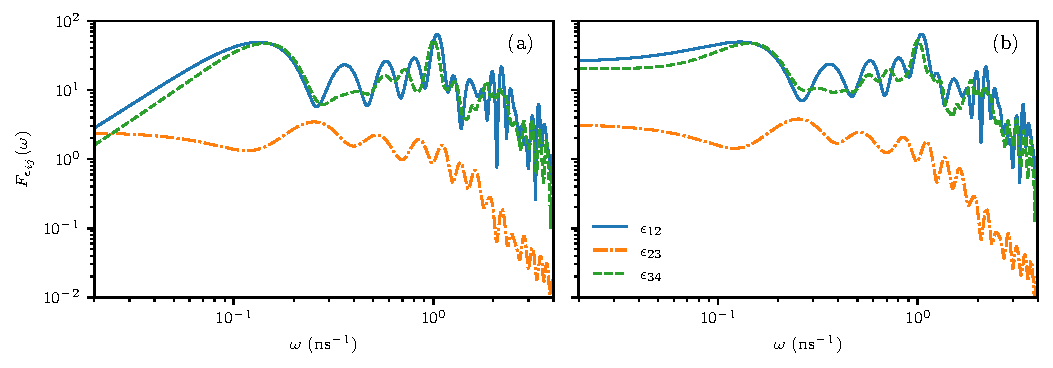
\includegraphics{img/pdf/filter_function-CNOT_unitary_v_complete}
    \caption{
        Filter functions of the voltage detunings $\epsilon_{ij}$ excluding (a) and including (b) the zero-padded identity matrix basis element $C_0^c\propto\text{diag}(1,1,1,1,0,0)$ for the computational subspace.
        Evidently, including $C_0^c$ removes the DCG character, namely that $F_{\epsilon_{ij}}(\omega)\rightarrow 0$ as $\omega\rightarrow 0$, of the gates but has little effect on the high-frequency behavior.
        As the pulse optimization minimizes, among other figures of merit, the infidelity of the final propagator mapped to the closest unitary on the computational subspace due to quasistatic and fast white noise, this indicates that excluding $C_0^c$ from the filter function corresponds to partially neglecting non-unitary components of the propagator on the computational subspace.
}
    \label{appfig:ff:filter_function:cnot}
\end{figure}

% ==================================================
%           QFT GATES SECTION
% ==================================================
\section{GRAPE-optimized gate set for QFT}\label{sec:app:ff:qft}
For completeness, in this appendix we give details on the GRAPE-optimized pulses for the gate set $\mathbb{G} = \lbrace\mr{X}_{i}(\flatfrac{\pi}{2}),\mr{Y}_{i}(\flatfrac{\pi}{2}),\mr{CR}_{ij}(\flatfrac{\pi}{2^3})\rbrace$ used in \cref{sec:ff:examples:qft} to simulate a \gls{qft} algorithm.
As mentioned in the main text, we consider a toy Rabi driving model with IQ single-qubit control and exchange to mediate inter-qubit coupling.
Cast in the language of quantum optimal control theory this translates to a vanishing drift (static) Hamiltonian, $H_\mr{d} =  0$, and a control Hamiltonian in the rotating frame given by
\begin{gather}
    \Hc(t) = \Hc\gth{0}(t)\otimes\eye + \eye\otimes\Hc\gth{1}(t) + \Hc\gth{01}(t), \\
    \Hc\gth{i}(t) = I_i(t)\px\gth{i} + Q_i(t)\py\gth{i},\qquad\Hc\gth{ij}(t) = J_{ij}(t)\pz\gth{i}\otimes\pz\gth{j},
\end{gather}
where $I_i(t)$ and $Q_i(t)$ are the in-phase and quadrature pulse envelopes and $\sigma_{x,y}\gth{i}$ are the Pauli matrices acting on the $i$-th and extended trivially to the other qubit.
As our goal is only of illustrative nature and not to provide a detailed gate optimization, we obtain the controls $\lbrace I_0(t), Q_0(t), I_1(t), Q_1(t), J_{12}(t)\rbrace$ for the gate set $\mathbb{G}$ using the GRAPE algorithm implemented in \qutip~\cite{Johansson2012} initialized with randomly distributed amplitudes.
The resulting pulses and the corresponding filter functions for the relevant noise operators are shown in \cref{appfig:ff:qft:gates}.

\begin{figure}
    \centering
    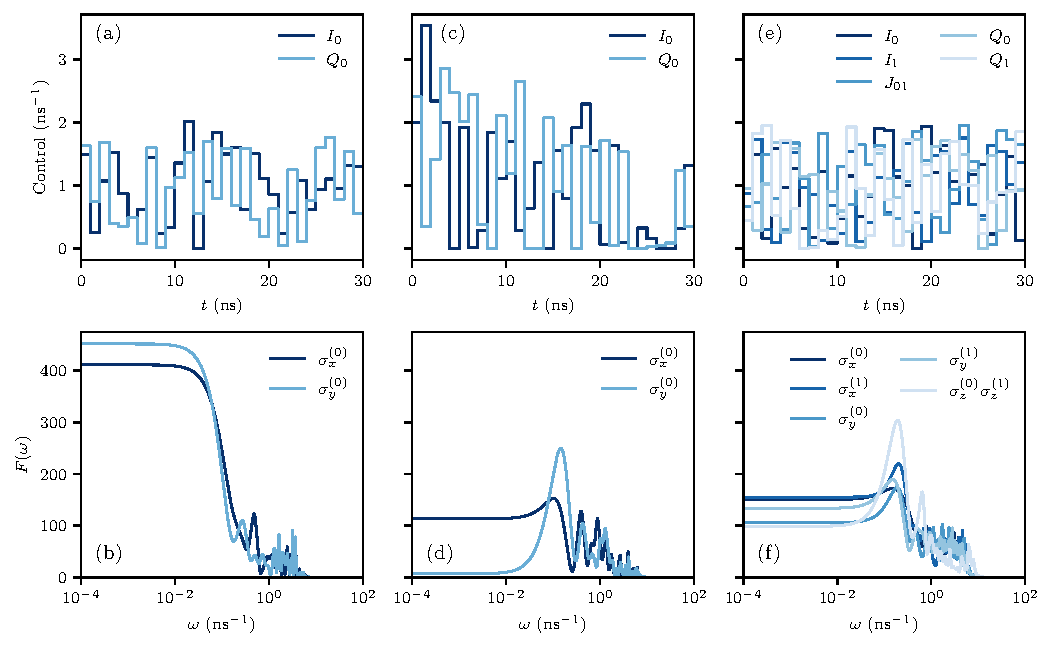
\includegraphics{img/pdf/qft_atomic_pulses}
    \caption{
        Control fields (top row) and corresponding filter functions (bottom row) of the GRAPE-optimized pulses in $\mathbb{G}$.
        (a),(b) $\text{X}_0(\flatfrac{\pi}{2})$; (c),(d) $\text{Y}_0(\flatfrac{\pi}{2})$; (e),(f) $\text{CR}_{01}(\flatfrac{\pi}{2^3})$.
        Note that the optimization is neither very sophisticated nor realistic as the algorithm only maximizes the systematic (coherent) fidelity $\mr{tr}\bigl(UQ\adjoint_\mr{targ}\bigr)/d$ and the randomly distributed initial control amplitudes are not subject to any constraints.
    }
    \label{appfig:ff:qft:gates}
\end{figure}

% ==================================================
%           CONVERGENCE SECTION
% ==================================================
\section{Convergence Bounds}\label{sec:app:ff:convergence}
In this appendix we give bounds for the convergence of the expansions employed in the main text for the case of purely auto-correlated noise, $S_{\alpha\beta}(\omega) = \delta_{\alpha\beta}S_{\alpha\beta}(\omega) =  S_\alpha(\omega)$, following the approach by~\citeauthor{Green2013}.
For Gaussian noise, our expansion is exact when including first and second order \acrfull{me} terms.
Hence, the convergence radius of the \gls{me} becomes infinite and the fidelity can be computed exactly by evaluating the matrix exponential \cref{eq:ff:cumulant}.
For non-Gaussian noise, the following considerations apply.
\subsection{Magnus Expansion}\label{sec:app:ff:convergence:magnus_expansion}
The \gls{me} of the error propagator \cref{eq:ff:magnus_expansion:1} converges if $\int_0^\tau\dd{t}\norm*{\Hnt(t)} < \pi$ with $\norm{A}^2 = \dotHS{A}{A} = \sum_{ij}\abs{A_{ij}}^2$ the Frobenius norm~\cite{Moan1999}.
We assume a time dependence of the noise operators of the form $\Ba(t) = s_\alpha(t)\Ba$.
By the Cauchy-Schwarz inequality we then have
\begin{equation}
    \begin{split}
        \bigl\lVert\Hnt(t)\bigr\rVert^2 &= \norm{\Hn(t)}^2 \\
                          &= \sum_{\alpha\beta} s_\alpha(t) s_{\beta}(t) b_\alpha(t) b_{\beta}(t)\dotHS{B_\alpha}{B_{\beta}} \\
                          &\leq\sum_{\alpha\beta} s_\alpha(t) s_{\beta}(t) b_\alpha(t) b_{\beta}(t)
                             \norm{B_\alpha}\norm{B_{\beta}} \\
                          &\leq\biggl[\sum_{\alpha}\sum_{g=1}^{G}\vartheta\gth{m}(t)
                             s_\alpha\gth{m}b_\alpha\gth{m}\norm{B_\alpha}\biggr]^2
    \end{split}
\end{equation}
where $b_{\alpha}\gth{m}$ is the maximum value that the noise assumes during the pulse, $\vartheta\gth{g}(t) = \theta(t - t_{g-1}) - \theta(t - t_g)$ is one during the $g$-th time interval and zero else, and where we approximated the time evolution as piecewise constant.
Then, in order to guarantee convergence of the \gls{me},
\begin{equation}
    \begin{split}
        \int_0^{\tau}\dd{t}\norm*{\Hnt(t)} &\leq\int_0^\tau\dd{t}\abs\bigg{\sum_{\alpha}\sum_{g=1}^{G}
                                              \vartheta\gth{m}(t) s_\alpha\gth{m} b_\alpha\gth{m}\norm{B_\alpha}} \\
                                           &= \sum_{\alpha} b_\alpha\gth{m}\norm{B_\alpha}\sum_{g=1}^{G}s_\alpha\gth{m}
                                              \int_{t_{g-1}}^{t_{g}}\dd{t} \\
                                           &= \sum_{\alpha} C_m\delta b_\alpha\norm{B_\alpha}\sum_{g=1}^{G}
                                              s_\alpha\gth{m}\Delta t_g \\
                                           &\eqqcolon N
    \end{split}
\end{equation}
where we have expressed the in principle unknown maximum noise amplitude $b_\alpha\gth{m}$ in terms of the root mean square value $\delta b_\alpha$.
That is, $b_\alpha\gth{m} = C_m \expval*{b_\alpha(0)^2}^{1/2} =  C_m \delta b_\alpha$ for a sufficiently large value $C_m$.
Finally, realizing that $\delta b_\alpha^2 = \int\frac{\dd{\omega}}{2\pi} S_\alpha(\omega)$ and by the triangle inequality,
\begin{equation}
    \begin{split}
        N &= C_m\sum_{\alpha}\norm{B_\alpha}\biggl[\int_{-\infty}^\infty\frac{\mathrm{d}\omega}{2\pi} S_\alpha(\omega)\biggr]^{1/2}
            \sum_{g=1}^{G} s_\alpha\gth{m}\Delta t_g \\
          &\leq C_m\biggl[\sum_{\alpha}\norm{B_\alpha}^2\int_{-\infty}^\infty\frac{\mathrm{d}\omega}{2\pi} S_\alpha(\omega)
            \biggl(\sum_{g=1}^{G} s_\alpha\gth{m}\Delta t_g\biggr)^2\biggr]^{1/2} \\
          &\eqqcolon C_m\xi \\
          &\overset{!}{<} \pi
    \end{split}
\end{equation}
where we have introduced the parameter $\xi$.
Thus, the expansion converges if $\xi < \flatfrac{\pi}{C_m}$.
However, we note that in practice the rms noise amplitude $\delta b_\alpha$ will often be infinite, limiting the usefulness of this bound for certain noise spectra.
\subsection{Infidelity}\label{sec:app:ff:convergence:infidelity}
Again assuming a time dependence $\Ba(t) = s_\alpha(t)\Ba$ as well as piecewise constant control, we note that for the infidelity we have (\cf \cref{eq:ff:fidelity:ent})
\begin{equation}
    \begin{split}
        \abs{\tr(\decayamps)} &= \abs\Bigg{\sum_{\alpha}\int_0^\tau\dd{t_2}\int_0^\tau\dd{t_1}
                                 \expval{b_\alpha(t_1)b_\alpha(t_2)}\sum_{k}\ctrlmat_{\alpha k}(t_1)\ctrlmat_{\alpha k}(t_2)} \\
                              &\leq\abs\Bigg{\sum_{\alpha}\int_0^\tau\dd{t_2}\int_0^\tau\dd{t_1}
                                 \expval{b_\alpha(t_1)b_\alpha(t_2)}\sum_{g,g'=1}^{G}\vartheta\gth{m}(t_1)\vartheta^{(g')}(t_2)
                                 s_\alpha\gth{m} s_\alpha^{(g')} \norm{B_\alpha}^2} \\
                              &\leq\sum_{\alpha}\norm{B_\alpha}^2
                                 \underbrace{\expval{b_\alpha^2(0)}}_{\int\frac{\dd{\omega}}{2\pi}S_\alpha(\omega)}
                                 \sum_{g,g'=1}^{G} s_\alpha\gth{m} s_\alpha^{(g')}
                                 \abs\Bigg{\int_{t_{g'-1}}^{t_{g'}}\dd{t_2}\int_{t_{g-1}}^{t_g}\dd{t_1}
                                 \underbrace{\overline{\expval{b_\alpha(t_1)b_\alpha(t_2)}}}_{\abs{\placeholder}\leq 1}} \\
                              &\leq\sum_{\alpha}\left[\norm{B_\alpha}^2
                                 \int_{-\infty}^\infty\frac{\mathrm{d}\omega}{2\pi}S_\alpha(\omega)
                                 \biggl(\sum_{g=1}^{G}s_\alpha\gth{m}\Delta t_g\biggr)^2\right] \\
                              &= \xi^2,
    \end{split}
\end{equation}
where, going from the second to the third line, we have factored out the total power of noise source $\alpha$ from the cross-correlation function, $\expval{b_\alpha(t_1) b_\alpha(t_2)} = \expval{b_\alpha^2(0)}\bigl\lvert\overline{\expval{b_\alpha(t_1)b_\alpha(t_2)}}\bigr\rvert$.
Thus, the first order infidelity \cref{eq:ff:fidelity:ent} is upper bounded by $\flatfrac{\xi^2}{d}$, the same parameter also bounding the convergence of the \gls{me}, and higher orders can be neglected if $\xi^2\ll 1$.

Note that similar arguments can be made for the higher orders of the \gls{me}~\cite{Green2013}.
In particular, the $n$-th order \gls{me} term containing $n$-point correlation functions of the noise is of order $\order{\xi^n}$ as stated in the main text.

\section{Second-order concatenation}\label{sec:app:ff:concatenation}
In this appendix, I lay out how the second-order filter functions of atomic pulse segments can be re-used to compute the filter function of the concatenated sequence.
While it is not possible, due to the nested time integral\todo{refeq}, to perform the calculation entirely without concern for the internal structure of the individual segments, it is also not necessary to compute everything from scratch.


%----------------------------------------------------------------------------------------

\backmatter % Denotes the end of the main document content
\setchapterstyle{plain} % Output plain chapters from this point onwards

%----------------------------------------------------------------------------------------
%	BIBLIOGRAPHY
%----------------------------------------------------------------------------------------

% The bibliography needs to be compiled with biber using your LaTeX editor, or on the command line with 'biber main' from the template directory

%\defbibnote{bibnote}{Here are the references in citation order.\par\bigskip} % Prepend this text to the bibliography
\printbibliography[
	heading=bibintoc,%
	title=Bibliography,
	%prenote=bibnote
] % Add the bibliography heading to the ToC, set the title of the bibliography and output the bibliography note

%----------------------------------------------------------------------------------------
%	GLOSSARY
%----------------------------------------------------------------------------------------

% The glossary needs to be compiled on the command line with 'makeglossaries main' from the template directory

\setglossarystyle{listgroup} % Set the style of the glossary (see https://en.wikibooks.org/wiki/LaTeX/Glossary for a reference)
\printglossary[title=Special Terms, toctitle=List of Terms] % Output the glossary, 'title' is the chapter heading for the glossary, toctitle is the table of contents heading

%----------------------------------------------------------------------------------------
%	INDEX
%----------------------------------------------------------------------------------------

% The index needs to be compiled on the command line with 'makeindex main' from the template directory

% \printindex % Output the index

%----------------------------------------------------------------------------------------
%	BACK COVER
%----------------------------------------------------------------------------------------

% If you have a PDF/image file that you want to use as a back cover, uncomment the following lines

%\clearpage
%\thispagestyle{empty}
%\null%
%\clearpage
%\inputpdf{cover-back.pdf}

%----------------------------------------------------------------------------------------

\end{document}
